\documentclass[a4paper]{book}
\usepackage{makeidx}
\usepackage{graphicx}
\usepackage{multicol}
\usepackage{float}
\usepackage{listings}
\usepackage{color}
\usepackage{ifthen}
\usepackage[table]{xcolor}
\usepackage{textcomp}
\usepackage{alltt}
\usepackage{ifpdf}
\ifpdf
\usepackage[pdftex,
            pagebackref=true,
            colorlinks=true,
            linkcolor=blue,
            unicode
           ]{hyperref}
\else
\usepackage[ps2pdf,
            pagebackref=true,
            colorlinks=true,
            linkcolor=blue,
            unicode
           ]{hyperref}
\usepackage{pspicture}
\fi
\usepackage[utf8]{inputenc}
\usepackage{mathptmx}
\usepackage[scaled=.90]{helvet}
\usepackage{courier}
\usepackage{doxygen}
\lstset{language=C++,inputencoding=utf8,basicstyle=\footnotesize,breaklines=true,breakatwhitespace=true,tabsize=6,numbers=left }
\makeindex
\setcounter{tocdepth}{3}
\renewcommand{\footrulewidth}{0.4pt}
\begin{document}
\hypersetup{pageanchor=false}
\begin{titlepage}
\vspace*{7cm}
\begin{center}
{\Large THE GAME \\[1ex]\large v0.5.1e }\\
\vspace*{1cm}
{\large Generated by Doxygen 1.7.3}\\
\vspace*{0.5cm}
{\small Fri Sep 27 2013 14:57:24}\\
\end{center}
\end{titlepage}
\clearemptydoublepage
\pagenumbering{roman}
\tableofcontents
\clearemptydoublepage
\pagenumbering{arabic}
\hypersetup{pageanchor=true}
\chapter{Belief Functions Implementation}
\label{index}\hypertarget{index}{}\hypertarget{index_intro_sec}{}\section{Introduction}\label{index_intro_sec}
This little library implements the basics to manipulate belief functions. The module BeliefsFromSensors enables the creation of belief functions from sensor measures. To run tests and a bench for speed of execution, please use the Tests module.

If some errors occur anywhere when running the tests, please check the format of the files in data/beliefs/. If you're stuck anywhere, feel free to send me an email. Different combination rules are implemented to enable the use in the case of different theories. The source code is documented AND commented (most of the time) to facilitate its reading. It is also under the Apache License v2 (\href{http://www.apache.org/licenses/LICENSE-2.0}{\tt http://www.apache.org/licenses/LICENSE-\/2.0}), thus, if any error/weird behaviour/bad coding is detected, please feel free to correct the source code and to notify me at one of the given email addresses given below. \par


If something you need is missing and you do not want/cannot contribute to the development, send me an email with your request and I will see what I can do for you! This library is meant to be as useful as possible! Anyway, please read the doc and specifically the description of modules, it should explain what it does.

This implementation of the basics of the belief functions theory has been created in order to test the applicability of this theory in specific cases. Thus, every part has not been developped yet! Anyway, a huge part of the work consisted in the optimization of the computations. Even if that's not perfert at all, a real effort has been done.

What it does: \begin{DoxyItemize}
\item Sets: creation and manipulation of sets (required for belief functions) and generation of powersets. \item Belief functions: manipulation, fusion, characterization and decision making from belief functions.\end{DoxyItemize}
The building of belief functions has been implemented in three cases: \begin{DoxyItemize}
\item Using raw sensor measures -\/-\/$>$ BeliefsFromSensors module \item Transforming belief functions -\/-\/$>$ BeliefsFromBeliefs module \item Random generation of belief functions -\/-\/$>$ BeliefsFromRandomness module\end{DoxyItemize}
\hypertarget{index_compil_sec}{}\section{Compilation}\label{index_compil_sec}
To compile, it is mandatory to include the math library (-\/lm) and the real-\/time library (-\/lrt). \par


The file \hyperlink{config_8h}{config.h} enables the configuration of compilation (Windows/Unix and debug or not). Once you are sure that everything is okay (sufficient memory, valid files, valid models), you can comment the DEBUG, CHECK\_\-SUM, CHECK\_\-VALUES, CHECK\_\-MODELS and CHECK\_\-COMPATIBILITY defines to gain in performance. \par
 The makefile is here to help you to compile everything. Replace the main by yours and just do a \char`\"{}make\char`\"{}. The default compilation options are quite constraining so feel free to remove some on them such as -\/pedantic...

If this is the first time you use this library, please have a look at the documentation or refer to the raw code given in \hyperlink{_tests_8c}{Tests.c} to see how the functions are used and called (a tutorial page is coming!).\hypertarget{index_ref_philo}{}\section{Philosophy of the implementation}\label{index_ref_philo}
It seems important to me to give more precision on how to use this little library and how it has been implemented.

The main idea in this library is that I don't want to lose any information at any time. Thus, all the functions that could modify mass functions create new ones instead! You have to free every new mass function that has been created. To create copies of mass function, there is a function called \hyperlink{_belief_functions_8c_ae248331ed725fe2bbba71abc0b397aab}{BF\_\-copyBeliefFunction()} which creates a hard copy of the given mass function. That is why most functions work with structures instead of pointers on structures.\hypertarget{index_ref_sec}{}\section{Main References}\label{index_ref_sec}
\begin{DoxyItemize}
\item A. Appriou -\/ Formulation et traitement de l'incertain en analyse multi-\/senseurs -\/ Quatorzieme Colloque GRETSI, Juan les Pins, 951-\/953 -\/ 1993 \item A. Appriou -\/ Multisensor Signal Processing in the Framework of the Theory of Evidence -\/ Application of Mathematical Signal Processing Techniques to Mission Systems, pages (5-\/1) (5 -\/ 31), Research and Technology Organization -\/ 1999 \item A. Appriou -\/ Approche generique de la gestion de l'incertain dans les processus de fusion multisenseur -\/ Traitement du Signal 22, 307-\/319 -\/ 2005 \item L.-\/Z. Chen, W.-\/K. Shi, Y. Deng, Z.-\/F. Zhu -\/ A new fusion approach based on distance of evidences -\/ Journal of Zhejiang University Science 61(5), pg 476-\/482 -\/ 2005 \item D. Dubois \& H. Prade -\/ Representation and combination of uncertainty with belief functions and possibility measures -\/ Computational intelligence 4, 244-\/264 -\/ 1988 \item R. Haenni and N. Lehmann -\/ Implementing belief function computations -\/ International Journal of Intelligent Systems volume 18, pg 31-\/49 -\/ 2003 \item A. Martin -\/ Modelisation et gestion du conflit dans la theorie des fonctions de croyance -\/ These d'Habilitation a Diriger des Recherches de l'Universite Occidentale -\/ 2009 \item C.K. Murphy -\/ Combining belief functions when evidence conflicts -\/ Decision support systems 29 1-\/9 -\/ 1999 \item B. Pietropaoli, M. Dominici, F. Weis -\/ Multi-\/sensor data fusion within the belief functions framework -\/ In S. Balandin, Y. Koucheryavy, H. Hu (eds.) NEW2AN, Lecture Notes in Computer Science, vol. 6869, pp. 123-\/134. Springer -\/ 2011 \item B. Pietropaoli, M. Dominici, F. Weis -\/ Belief Inference with Timed Evidence : Methodology and Application using Sensors in a Smart Home -\/ Proceedings of Belief 2012, Compiegne, France, 9-\/11 May -\/ 2012 \item V. Ricquebourg, M. Delafosse, L. Delahoche, B. Marhic, A. Jolly-\/Desodt, D. Menga, -\/ Fault Detection by Combining Redundant Sensors: a Conflict ApproachWithin the TBM Framework. In COGIS 2007, COGnitive systems with Interactive Sensors. Stanford University -\/ 2007 \item G. Shafer -\/ A mathematical theory of evidence -\/ Princeton University Press, Princeton, NJ, 1976 \item Ph. Smets and R. Kruse -\/ The Transferable Belief Model for Belief Representation -\/ Smets Ph. and Motro A. eds. Uncertainty Management in information systems: from needs to solutions. UMIS Workshop, Puerto Andraix.Volume 2. pg 91-\/111 -\/ 1993 \item Ph. Smets -\/ The transferable belief model for quantified belief representation -\/ In D. M. Gabbay \& P. Smets (Eds.), Handbook of defeasible reasoning and uncertainty management -\/ 1998 \item Ph. Smets -\/ Theories of Uncertainty -\/ Handbook of fuzzy computing, Section B.1.1.2 -\/ 1995 \item P. Vannoorenberghe -\/ Un etat de l'art sur les fonctions de croyance appliquees au traitement de l'information -\/ 2002 \item R.R. Yager -\/ On the Dempster-\/Shafer framework and new combination rules -\/ Information Sciences 41, 93-\/138 -\/ 1987 \item ... and more I'm sure I forgot... (Anyway, you should find it in the doc of concerned functions if required...) In any case, this theory is HUGE and it is hard to cite everything you can find on it!\end{DoxyItemize}
\hypertarget{index_contact_sec}{}\section{Contact}\label{index_contact_sec}
Bastien Pietropaoli \par
 Ph.D. student \par
 INRIA, Rennes -\/ Bretagne Atlantique \par
 ACES Team \par


{\bfseries Email:} \par
 \href{mailto:bastien.pietropaoli@inria.fr}{\tt bastien.pietropaoli@inria.fr} \par
 \href{mailto:bastien.pietropaoli@gmail.com}{\tt bastien.pietropaoli@gmail.com} \par


Copyright 2011-\/2013, EDF. This software was developed with the collaboration of INRIA (Bastien Pietropaoli) 
\chapter{Version notes}
\label{version_sec}
\hypertarget{version_sec}{}
\hypertarget{version_sec_v02_subsec}{}\section{V0.\-2}\label{version_sec_v02_subsec}
New operations are now available\-: \begin{DoxyItemize}
\item discounting() \-: This function corresponds to the classical discounting operation. The lost belief is transferred on the complete universe. \item $\ast$\-Combination() and full$\ast$\-Combination() \-: These functions implements the different combination rules proposed in the belief functions framework Two functions have been modified\-: combination() and full\-Combination(). They now take an argument concerning the type of combination rule to use.\end{DoxyItemize}
\hypertarget{version_sec_v03_subsec}{}\section{V0.\-3}\label{version_sec_v03_subsec}
Name of operations have been corrected. The implementation of sets has been optimized a lot (exec time divided by 2 and a lot of memory saved). The implementation is totally mem-\/check free (checked with Valgrind) !\hypertarget{version_sec_v03_1_subsec}{}\section{V0.\-3.\-1}\label{version_sec_v03_1_subsec}
An emulation of namespace has been added in modules for function names. Minor bugs have been corrected.\hypertarget{version_sec_v03_2_subsec}{}\section{V0.\-3.\-2}\label{version_sec_v03_2_subsec}
The pure B\-F\-T has been separated from the application with sensors. Thus, the belief building from sensor measures has been put in a new specific file called Beliefs\-From\-Sensors(.h and .c).\hypertarget{version_sec_v04_subsec}{}\section{V0.\-4}\label{version_sec_v04_subsec}
New functionalities\-: \begin{DoxyItemize}
\item Options\-: It is now possible to add options to the belief model adding a file called 'options' with the files containing the points for sets of belief functions. The file should contain one option per line composed of a name of option and a float parameter. Only variation and tempo are now available. \item Decision support functions\-: those functions implemented in Belief\-Functions module enable to find a max or a min of a belief function for mass, belief and plausibility. The implementation is totally mem-\/check free (checked with Valgrind) !\end{DoxyItemize}
\hypertarget{version_sec_v04_1_subsec}{}\section{V0.\-4.\-1}\label{version_sec_v04_1_subsec}
Correction of the function used to measure time in the tempo option. (Use of clock\-\_\-gettime(C\-L\-O\-C\-K\-\_\-\-R\-E\-A\-L\-T\-I\-M\-E,...) now) \par
 Adding \hyperlink{_sets_8c_a7693e000c2760240139628cd1b33d2f1}{Sets\-\_\-element\-To\-Bit\-String()} in Sets module. \par
 Adding the D\-E\-B\-U\-G, C\-H\-E\-C\-K\-\_\-\-S\-U\-M and C\-H\-E\-C\-K\-\_\-\-V\-A\-L\-U\-E\-S defines in \hyperlink{config_8h}{config.\-h} to customize the compilation and optimize a little more the execution time. \par
 The implementation is totally mem-\/check free (checked with Valgrind) !\hypertarget{version_sec_v04_2_subsec}{}\section{V0.\-4.\-2}\label{version_sec_v04_2_subsec}
Adding \hyperlink{_sets_8c_ab9ee97ae54608f3fb5784b29503d62b6}{Sets\-\_\-element\-From\-Number()} and \hyperlink{_sets_8c_a71aeb52bad651c5129b57d7e69e5f480}{Sets\-\_\-number\-From\-Element()} in Sets module. \par
 Correction of a bug in the function \hyperlink{_sets_8c_a7693e000c2760240139628cd1b33d2f1}{Sets\-\_\-element\-To\-Bit\-String()}. \par
 Addition of a function \hyperlink{_sets_8c_a76fd7c759c8e24d17fdc240cc003c969}{Sets\-\_\-set\-To\-Bit\-String()}. \par
 Separation of the temporization in a new function B\-F\-S\-\_\-temporization() instead of doing it directly in \hyperlink{_beliefs_from_sensors_8c_a0e545c6a35093eb43b27325db61c2216}{B\-F\-S\-\_\-get\-Projection()}. \par
 Code of the function \hyperlink{_beliefs_from_sensors_8c_a0e545c6a35093eb43b27325db61c2216}{B\-F\-S\-\_\-get\-Projection()} cleaned up. \par
 In \hyperlink{_beliefs_from_sensors_8c_a0e545c6a35093eb43b27325db61c2216}{B\-F\-S\-\_\-get\-Projection()}, if sensor\-Measure == W\-E\-I\-R\-D\-\_\-\-N\-U\-M\-B\-E\-R, then the projection equals the vacuous belief function. The temporization is done anyway. It's really usefull if you replace a lost measure by this W\-E\-I\-R\-D\-\_\-\-N\-U\-M\-B\-E\-R because you'll get the vacuous or a trace of the last belief using the temporization. \par
 The Belief\-Functions module has been cleaned of all the \char`\"{}element\-Size\char`\"{} by putting this variable inside the \hyperlink{struct_b_f___belief_function}{B\-F\-\_\-\-Belief\-Function} structure. \par
 Diverse things have been renamed to be more explicit and/or more convenient for the extension of the library. \par
 The implementation is totally mem-\/check free (checked with Valgrind) ! \par
\hypertarget{version_sec_v05_subsec}{}\section{V0.\-5}\label{version_sec_v05_subsec}
Addition of a new applicative module Beliefs\-From\-Beliefs. \par
 Minor changes in diverse modules (that's the spirit of uncertain modification \-:)). \par
 Addition of a new function to clean the \hyperlink{struct_b_f___belief_function}{B\-F\-\_\-\-Belief\-Function} of non-\/focal elements. \par
 Addition of a new way of doing temporization using Dubois \& Prade's combination rule instead of a discrimination based on specificity. \par
 In the module Beliefs\-From\-Sensors, the options are now managed using flags, thus it should be easier to add and manage new options! \par
 The implementation is totally mem-\/check free (checked with Valgrind) ! \par
\hypertarget{version_sec_v051_subsec}{}\section{V0.\-5.\-1}\label{version_sec_v051_subsec}
Addition of a new function to normalize the B\-F\-\_\-\-Belief\-Functions. \par
 Addition of a new applicative module Beliefs\-From\-Randomness (in progress...) \par
 Some things have been renamed to be more explicit. \par
 No more warnings! (compiling well with -\/\-Wall -\/\-Wextra -\/\-Werror -\/pedantic) \par
 In \hyperlink{_beliefs_from_sensors_8h}{Beliefs\-From\-Sensors.\-h}, a new define has been added to enable the use of different clocks for the temporization. It is useful when working on diverse O\-S implementing different clocks. \par
 Some combination rules have been reimplemented to increase performance and this is much better ! (I got rid of the dirty code of the beginning of the project...) \par
 The implementation is totally mem-\/check free (checked with Valgrind) ! \par
\hypertarget{version_sec_Version_contact}{}\section{Contact}\label{version_sec_Version_contact}
Bastien Pietropaoli \par
 Ph.\-D. student \par
 I\-N\-R\-I\-A, Rennes -\/ Bretagne Atlantique \par
 A\-C\-E\-S Team \par


{\bfseries Email\-:} \par
 \href{mailto:bastien.pietropaoli@inria.fr}{\tt bastien.\-pietropaoli@inria.\-fr} \par
 \href{mailto:bastien.pietropaoli@gmail.com}{\tt bastien.\-pietropaoli@gmail.\-com} \par


Copyright 2011-\/2013, E\-D\-F. This software was developed with the collaboration of I\-N\-R\-I\-A (Bastien Pietropaoli) 
\chapter{TODO Page}
\label{TODO}
\hypertarget{TODO}{}
\hypertarget{_t_o_d_o_TODO_Intro}{}\section{Introduction}\label{_t_o_d_o_TODO_Intro}
If you feel in the mood to enjoy some C code, on this page, you can find a list a things to do to improve this library.\hypertarget{_t_o_d_o_Todo_list}{}\section{Todo list}\label{_t_o_d_o_Todo_list}
\begin{DoxyItemize}
\item Implement new combination rules (PCR5/6, Florea, etc...) \item Implement new applicative modules \item Implement other theories (multi-\/frame functions, continuous belief function, DSmT, etc...) \item Add some tools to build belief functions (randomly, from certain files, from statistics, etc...)\end{DoxyItemize}
\hypertarget{_t_o_d_o_Todo_contact}{}\section{Contact}\label{_t_o_d_o_Todo_contact}
Bastien Pietropaoli \par
 Ph.D. student \par
 INRIA, Rennes -\/ Bretagne Atlantique \par
 ACES Team \par


{\bfseries Email:} \par
 \href{mailto:bastien.pietropaoli@inria.fr}{\tt bastien.pietropaoli@inria.fr} \par
 \href{mailto:bastien.pietropaoli@gmail.com}{\tt bastien.pietropaoli@gmail.com} \par
 
\chapter{Origin of the name}
\label{origin_page}
\hypertarget{origin_page}{}
I lost...

\href{http://en.wikipedia.org/wiki/The_Game_(mind_game)}{\tt http://en.wikipedia.org/wiki/The\_\-Game\_\-(mind\_\-game)}\hypertarget{origin_page_Origin_contact}{}\section{Contact}\label{origin_page_Origin_contact}
Bastien Pietropaoli \par
 Ph.D. student \par
 INRIA, Rennes -\/ Bretagne Atlantique \par
 ACES Team \par


{\bfseries Email:} \par
 \href{mailto:bastien.pietropaoli@inria.fr}{\tt bastien.pietropaoli@inria.fr} \par
 \href{mailto:bastien.pietropaoli@gmail.com}{\tt bastien.pietropaoli@gmail.com} \par


Copyright 2011-\/2013, EDF. This software was developed with the collaboration of INRIA (Bastien Pietropaoli) 
\chapter{FAQ}
\label{FAQ_page}
\hypertarget{FAQ_page}{}
As sometimes, we got a question, the frequently asked question section may contain the answer we are looking for.\hypertarget{_f_a_q_page_FAQ_character}{}\section{The names of my states are badly cut or contain $^\wedge$\-M characters}\label{_f_a_q_page_FAQ_character}
This is due to the end of line character difference between Windows and Linux/\-Mac\-O\-S. It counts for two characters on certain systems and for only one on others. To correct this, you can try to compile with another system variable (W\-I\-N\-D\-O\-W\-S or L\-I\-N\-U\-X).

For Linux users, it is also possible to get a package called \char`\"{}tofrodos\char`\"{} which enables to convert files from windows to linux format and vice versa.\hypertarget{_f_a_q_page_FAQ_contact}{}\section{Contact}\label{_f_a_q_page_FAQ_contact}
Bastien Pietropaoli \par
 Ph.\-D. student \par
 I\-N\-R\-I\-A, Rennes -\/ Bretagne Atlantique \par
 A\-C\-E\-S Team \par


{\bfseries Email\-:} \par
 \href{mailto:bastien.pietropaoli@inria.fr}{\tt bastien.\-pietropaoli@inria.\-fr} \par
 \href{mailto:bastien.pietropaoli@gmail.com}{\tt bastien.\-pietropaoli@gmail.\-com} \par


Copyright 2011-\/2013, E\-D\-F. This software was developed with the collaboration of I\-N\-R\-I\-A (Bastien Pietropaoli) 
\chapter{Quick start and tutorial}
\label{Tuto_page}
\hypertarget{Tuto_page}{}
This page is still under construction.\hypertarget{_tuto_page_ref_hard}{}\section{Starting the hard way}\label{_tuto_page_ref_hard}
I know some people like to code the hard way. If you want to build everything by yourself, this is an example of how it is possible to build a mass function from scratch. It also presents how to combine mass functions. (Note that if you keep the -\/pedantic option in the makefile, you should write the comments using /($\ast$) comments instead of // comments.) 
\begin{DoxyCode}
\hyperlink{struct_b_f___belief_function}{BF\_BeliefFunction} m, m2, m3;
\textcolor{keywordtype}{char}* str = NULL;
\textcolor{keywordtype}{char} bits[2], bits2[2];

\textcolor{comment}{//A two bits element:}
bits[0] = 1;
bits[1] = 1;

\textcolor{comment}{//Another two bits element: }
bits2[0] = 1;
bits2[1] = 0;

\textcolor{comment}{//Building a mass function the hard way: }
m.elementSize = 2;
m.nbFocals = 2;
m.focals = malloc(\textcolor{keyword}{sizeof}(\hyperlink{struct_b_f___focal_element}{BF\_FocalElement}) * 2);
m.focals[0].element = \hyperlink{_sets_8c_a734e81728f1e2e9fab1b86045dcc42d4}{Sets\_createElementFromBits}(bits, 2);
m.focals[0].beliefValue = 0.3;
m.focals[1].element = \hyperlink{_sets_8c_a734e81728f1e2e9fab1b86045dcc42d4}{Sets\_createElementFromBits}(bits2, 2);
m.focals[1].beliefValue = 0.7;

\textcolor{comment}{//Printing the mass function: }
str = \hyperlink{_belief_functions_8c_a09113849ea5c4042faebfd9c2b53e1b5}{BF\_beliefFunctionToBitString}(m);
printf(\textcolor{stringliteral}{"m = \(\backslash\)n%s\(\backslash\)n"}, str);
free(str);

\textcolor{comment}{//Combination of mass functions: }
m2 = \hyperlink{_belief_functions_8c_a34a15102ee96fc30396ef8972b99c440}{BF\_DempsterCombination}(m, m);
m3 = \hyperlink{_belief_functions_8c_a34a15102ee96fc30396ef8972b99c440}{BF\_DempsterCombination}(m2, m);

\textcolor{comment}{//Printing the result of combination: }
str = \hyperlink{_belief_functions_8c_a09113849ea5c4042faebfd9c2b53e1b5}{BF\_beliefFunctionToBitString}(m2);
printf(\textcolor{stringliteral}{"m2 = \(\backslash\)n%s\(\backslash\)n"}, str);
free(str);

str = \hyperlink{_belief_functions_8c_a09113849ea5c4042faebfd9c2b53e1b5}{BF\_beliefFunctionToBitString}(m3);
printf(\textcolor{stringliteral}{"m3 = \(\backslash\)n%s\(\backslash\)n"}, str);
free(str);

\textcolor{comment}{//Freeing mass functions: }
\hyperlink{_belief_functions_8c_aa3c5107945acc34941aed1c7f7e04968}{BF\_freeBeliefFunction}(&m);
\hyperlink{_belief_functions_8c_aa3c5107945acc34941aed1c7f7e04968}{BF\_freeBeliefFunction}(&m2);
\hyperlink{_belief_functions_8c_aa3c5107945acc34941aed1c7f7e04968}{BF\_freeBeliefFunction}(&m3);
\end{DoxyCode}
\hypertarget{_tuto_page_Tuto_contact}{}\section{Contact}\label{_tuto_page_Tuto_contact}
Bastien Pietropaoli \par
 Ph.\-D. student \par
 I\-N\-R\-I\-A, Rennes -\/ Bretagne Atlantique \par
 A\-C\-E\-S Team \par


{\bfseries Email\-:} \par
 \href{mailto:bastien.pietropaoli@inria.fr}{\tt bastien.\-pietropaoli@inria.\-fr} \par
 \href{mailto:bastien.pietropaoli@gmail.com}{\tt bastien.\-pietropaoli@gmail.\-com} \par


Copyright 2011-\/2013, E\-D\-F. This software was developed with the collaboration of I\-N\-R\-I\-A (Bastien Pietropaoli) 
\chapter{Data Structure Index}
\section{Data Structures}
Here are the data structures with brief descriptions:\begin{DoxyCompactList}
\item\contentsline{section}{\hyperlink{struct_b_f___belief_function}{BF\_\-BeliefFunction} }{\pageref{struct_b_f___belief_function}}{}
\item\contentsline{section}{\hyperlink{struct_b_f___focal_element}{BF\_\-FocalElement} }{\pageref{struct_b_f___focal_element}}{}
\item\contentsline{section}{\hyperlink{struct_b_f_b___belief_from_belief}{BFB\_\-BeliefFromBelief} }{\pageref{struct_b_f_b___belief_from_belief}}{}
\item\contentsline{section}{\hyperlink{struct_b_f_b___belief_structure}{BFB\_\-BeliefStructure} }{\pageref{struct_b_f_b___belief_structure}}{}
\item\contentsline{section}{\hyperlink{struct_b_f_b___belief_vector}{BFB\_\-BeliefVector} }{\pageref{struct_b_f_b___belief_vector}}{}
\item\contentsline{section}{\hyperlink{struct_b_f_s___belief_structure}{BFS\_\-BeliefStructure} }{\pageref{struct_b_f_s___belief_structure}}{}
\item\contentsline{section}{\hyperlink{struct_b_f_s___option}{BFS\_\-Option} }{\pageref{struct_b_f_s___option}}{}
\item\contentsline{section}{\hyperlink{struct_b_f_s___part_of_belief}{BFS\_\-PartOfBelief} }{\pageref{struct_b_f_s___part_of_belief}}{}
\item\contentsline{section}{\hyperlink{struct_b_f_s___point}{BFS\_\-Point} }{\pageref{struct_b_f_s___point}}{}
\item\contentsline{section}{\hyperlink{struct_b_f_s___sensor_beliefs}{BFS\_\-SensorBeliefs} }{\pageref{struct_b_f_s___sensor_beliefs}}{}
\item\contentsline{section}{\hyperlink{union_b_f_s___util_data}{BFS\_\-UtilData} }{\pageref{union_b_f_s___util_data}}{}
\item\contentsline{section}{\hyperlink{struct_sets___element}{Sets\_\-Element} }{\pageref{struct_sets___element}}{}
\item\contentsline{section}{\hyperlink{struct_sets___reference_list}{Sets\_\-ReferenceList} }{\pageref{struct_sets___reference_list}}{}
\item\contentsline{section}{\hyperlink{struct_sets___set}{Sets\_\-Set} }{\pageref{struct_sets___set}}{}
\end{DoxyCompactList}

\chapter{File Index}
\section{File List}
Here is a list of all documented files with brief descriptions:\begin{DoxyCompactList}
\item\contentsline{section}{\hyperlink{_belief_functions_8c}{BeliefFunctions.c} (CORE: Gives structures and main functions to manipulate belief functions )}{\pageref{_belief_functions_8c}}{}
\item\contentsline{section}{\hyperlink{_belief_functions_8h}{BeliefFunctions.h} (CORE: Gives structures and main functions to manipulate belief functions )}{\pageref{_belief_functions_8h}}{}
\item\contentsline{section}{\hyperlink{_beliefs_from_beliefs_8c}{BeliefsFromBeliefs.c} (APPLICATION: Gives structures and main functions to create belief functions from belief functions )}{\pageref{_beliefs_from_beliefs_8c}}{}
\item\contentsline{section}{\hyperlink{_beliefs_from_beliefs_8h}{BeliefsFromBeliefs.h} (APPLICATION: Gives structures and main functions to create belief functions from belief functions )}{\pageref{_beliefs_from_beliefs_8h}}{}
\item\contentsline{section}{\hyperlink{_beliefs_from_randomness_8c}{BeliefsFromRandomness.c} (APPLICATION: Gives structures and main functions to create random belief functions )}{\pageref{_beliefs_from_randomness_8c}}{}
\item\contentsline{section}{\hyperlink{_beliefs_from_randomness_8h}{BeliefsFromRandomness.h} (APPLICATION: Gives structures and main functions to create random belief functions )}{\pageref{_beliefs_from_randomness_8h}}{}
\item\contentsline{section}{\hyperlink{_beliefs_from_sensors_8c}{BeliefsFromSensors.c} (APPLICATION: Gives structures and main functions to create belief functions from sensor measures )}{\pageref{_beliefs_from_sensors_8c}}{}
\item\contentsline{section}{\hyperlink{_beliefs_from_sensors_8h}{BeliefsFromSensors.h} (APPLICATION: Gives structures and main functions to create belief functions from sensor measures )}{\pageref{_beliefs_from_sensors_8h}}{}
\item\contentsline{section}{\hyperlink{config_8h}{config.h} (UTILITY: A file to config the compilation )}{\pageref{config_8h}}{}
\item\contentsline{section}{{\bfseries main.c} }{\pageref{main_8c}}{}
\item\contentsline{section}{\hyperlink{_read_directory_8c}{ReadDirectory.c} (UTILITY: A module to ease the manipulation of directories )}{\pageref{_read_directory_8c}}{}
\item\contentsline{section}{\hyperlink{_read_directory_8h}{ReadDirectory.h} (UTILITY: A module to ease the manipulation of directories )}{\pageref{_read_directory_8h}}{}
\item\contentsline{section}{\hyperlink{_read_file_8c}{ReadFile.c} (UTILITY: A module to ease file reading )}{\pageref{_read_file_8c}}{}
\item\contentsline{section}{\hyperlink{_read_file_8h}{ReadFile.h} (UTILITY: A module to ease file reading )}{\pageref{_read_file_8h}}{}
\item\contentsline{section}{\hyperlink{_sets_8c}{Sets.c} (CORE: Implements the basics required to work on sets and elements in the theory of belief functions )}{\pageref{_sets_8c}}{}
\item\contentsline{section}{\hyperlink{_sets_8h}{Sets.h} (CORE: Implements the basics required to work on sets and elements in the theory of belief functions )}{\pageref{_sets_8h}}{}
\item\contentsline{section}{\hyperlink{_tests_8c}{Tests.c} (TESTS: Run runTests() to test that everything works fine on your configuration )}{\pageref{_tests_8c}}{}
\item\contentsline{section}{\hyperlink{_tests_8h}{Tests.h} (TESTS: Run runTests() to test that everything works fine on your configuration )}{\pageref{_tests_8h}}{}
\end{DoxyCompactList}

\chapter{Data Structure Documentation}
\hypertarget{struct_b_f___belief_function}{\section{B\-F\-\_\-\-Belief\-Function Struct Reference}
\label{struct_b_f___belief_function}\index{B\-F\-\_\-\-Belief\-Function@{B\-F\-\_\-\-Belief\-Function}}
}


{\ttfamily \#include $<$Belief\-Functions.\-h$>$}

\subsection*{Data Fields}
\begin{DoxyCompactItemize}
\item 
\hypertarget{struct_b_f___belief_function_af15d8fa92e4335a67d6947121b56f73f}{\hyperlink{struct_b_f___focal_element}{B\-F\-\_\-\-Focal\-Element} $\ast$ {\bfseries focals}}\label{struct_b_f___belief_function_af15d8fa92e4335a67d6947121b56f73f}

\item 
\hypertarget{struct_b_f___belief_function_a209e36604b4b97610dce90748bc70382}{int {\bfseries nb\-Focals}}\label{struct_b_f___belief_function_a209e36604b4b97610dce90748bc70382}

\item 
\hypertarget{struct_b_f___belief_function_abea30052ee8578b9752a41b244653914}{int {\bfseries element\-Size}}\label{struct_b_f___belief_function_abea30052ee8578b9752a41b244653914}

\end{DoxyCompactItemize}


\subsection{Detailed Description}
The real belief function. There are several ways to build belief functions (for instance using the Beliefs\-From\-Sensors module). Operations defined in this module are for mass functions but this structure can be used to store credibility or plausibility as well. 
\begin{DoxyParams}{Parameters}
{\em focals} & The focal elements of the mass function \\
\hline
{\em nb\-Focals} & The number of focals \\
\hline
{\em element\-Size} & The number of possible worlds in the frame of discernment. \\
\hline
\end{DoxyParams}


Definition at line 82 of file Belief\-Functions.\-h.



The documentation for this struct was generated from the following file\-:\begin{DoxyCompactItemize}
\item 
/home/arichez/git/\-T\-H\-E\-G\-A\-M\-E/src/main/include/\hyperlink{_belief_functions_8h}{Belief\-Functions.\-h}\end{DoxyCompactItemize}

\hypertarget{struct_b_f___focal_element}{
\section{BF\_\-FocalElement Struct Reference}
\label{struct_b_f___focal_element}\index{BF\_\-FocalElement@{BF\_\-FocalElement}}
}


{\ttfamily \#include $<$BeliefFunctions.h$>$}

\subsection*{Data Fields}
\begin{DoxyCompactItemize}
\item 
\hypertarget{struct_b_f___focal_element_a9a710ad49ddbc706371fa96ab1d1a4fa}{
\hyperlink{struct_sets___element}{Sets\_\-Element} {\bfseries element}}
\label{struct_b_f___focal_element_a9a710ad49ddbc706371fa96ab1d1a4fa}

\item 
\hypertarget{struct_b_f___focal_element_a59bb288073cdc2754b6d0ebc93b478d0}{
float {\bfseries beliefValue}}
\label{struct_b_f___focal_element_a59bb288073cdc2754b6d0ebc93b478d0}

\end{DoxyCompactItemize}


\subsection{Detailed Description}
A couple (element, belief) to associate a belief to an element. 
\begin{DoxyParams}{Parameters}
{\em elements} & The focal elements \\
\hline
{\em beliefValues} & The belief on each element (in the same order) \\
\hline
\end{DoxyParams}


Definition at line 64 of file BeliefFunctions.h.



The documentation for this struct was generated from the following file:\begin{DoxyCompactItemize}
\item 
\hyperlink{_belief_functions_8h}{BeliefFunctions.h}\end{DoxyCompactItemize}

\hypertarget{struct_b_f_b___belief_from_belief}{\section{B\-F\-B\-\_\-\-Belief\-From\-Belief Struct Reference}
\label{struct_b_f_b___belief_from_belief}\index{B\-F\-B\-\_\-\-Belief\-From\-Belief@{B\-F\-B\-\_\-\-Belief\-From\-Belief}}
}


{\ttfamily \#include $<$Beliefs\-From\-Beliefs.\-h$>$}

\subsection*{Data Fields}
\begin{DoxyCompactItemize}
\item 
\hypertarget{struct_b_f_b___belief_from_belief_ab587a94be97e747de0805ad46f879ee1}{char $\ast$ {\bfseries frame\-Name}}\label{struct_b_f_b___belief_from_belief_ab587a94be97e747de0805ad46f879ee1}

\item 
\hypertarget{struct_b_f_b___belief_from_belief_a049bf9892d2d4204a553cdc04c82047e}{\hyperlink{struct_sets___reference_list}{Sets\-\_\-\-Reference\-List} {\bfseries ref\-List}}\label{struct_b_f_b___belief_from_belief_a049bf9892d2d4204a553cdc04c82047e}

\item 
\hypertarget{struct_b_f_b___belief_from_belief_a770ef176fded84146981fda0900d1720}{\hyperlink{struct_b_f_b___belief_vector}{B\-F\-B\-\_\-\-Belief\-Vector} $\ast$ {\bfseries vectors}}\label{struct_b_f_b___belief_from_belief_a770ef176fded84146981fda0900d1720}

\item 
\hypertarget{struct_b_f_b___belief_from_belief_ae4e6e0fb7917cfb1b966b61085844c75}{int {\bfseries nb\-Vectors}}\label{struct_b_f_b___belief_from_belief_ae4e6e0fb7917cfb1b966b61085844c75}

\end{DoxyCompactItemize}


\subsection{Detailed Description}
The matrix to convert belief on a frame of discernment in a belief on another frame of discernment. 
\begin{DoxyParams}{Parameters}
{\em frame\-Name} & The name of the frame of discernment from which we start \\
\hline
{\em ref\-List} & The reference list for the explicitation of the states names in the frame \\
\hline
{\em vectors} & The list of vectors corresponding to the matrix \\
\hline
\end{DoxyParams}


Definition at line 153 of file Beliefs\-From\-Beliefs.\-h.



The documentation for this struct was generated from the following file\-:\begin{DoxyCompactItemize}
\item 
/home/arichez/git/\-T\-H\-E\-G\-A\-M\-E/src/main/include/\hyperlink{_beliefs_from_beliefs_8h}{Beliefs\-From\-Beliefs.\-h}\end{DoxyCompactItemize}

\hypertarget{struct_b_f_b___belief_structure}{
\section{BFB\_\-BeliefStructure Struct Reference}
\label{struct_b_f_b___belief_structure}\index{BFB\_\-BeliefStructure@{BFB\_\-BeliefStructure}}
}


{\ttfamily \#include $<$BeliefsFromBeliefs.h$>$}

\subsection*{Data Fields}
\begin{DoxyCompactItemize}
\item 
\hypertarget{struct_b_f_b___belief_structure_ab587a94be97e747de0805ad46f879ee1}{
char $\ast$ {\bfseries frameName}}
\label{struct_b_f_b___belief_structure_ab587a94be97e747de0805ad46f879ee1}

\item 
\hypertarget{struct_b_f_b___belief_structure_a049bf9892d2d4204a553cdc04c82047e}{
\hyperlink{struct_sets___reference_list}{Sets\_\-ReferenceList} {\bfseries refList}}
\label{struct_b_f_b___belief_structure_a049bf9892d2d4204a553cdc04c82047e}

\item 
\hypertarget{struct_b_f_b___belief_structure_adeef55dd9dfab2c8d381187222929087}{
\hyperlink{struct_b_f_b___belief_from_belief}{BFB\_\-BeliefFromBelief} $\ast$ {\bfseries beliefs}}
\label{struct_b_f_b___belief_structure_adeef55dd9dfab2c8d381187222929087}

\item 
\hypertarget{struct_b_f_b___belief_structure_a967b20b9b68b8e2dbb341c68a64ee7c4}{
int {\bfseries nbBeliefs}}
\label{struct_b_f_b___belief_structure_a967b20b9b68b8e2dbb341c68a64ee7c4}

\end{DoxyCompactItemize}


\subsection{Detailed Description}
The complete belief structure with all the beliefs of all the other belief on which it is possible to build metabelief. 
\begin{DoxyParams}{Parameters}
{\em frameName} & The name of the context attribute we want to compute \\
\hline
{\em refList} & The \hyperlink{struct_sets___reference_list}{Sets\_\-ReferenceList} corresponding to the real values of the context attribute \\
\hline
{\em beliefs} & The model of belief to get the context attribute value \\
\hline
{\em nbSensors} & The number of sensors in the structure \\
\hline
\end{DoxyParams}


Definition at line 174 of file BeliefsFromBeliefs.h.



The documentation for this struct was generated from the following file:\begin{DoxyCompactItemize}
\item 
\hyperlink{_beliefs_from_beliefs_8h}{BeliefsFromBeliefs.h}\end{DoxyCompactItemize}

\hypertarget{struct_b_f_b___belief_vector}{
\section{BFB\_\-BeliefVector Struct Reference}
\label{struct_b_f_b___belief_vector}\index{BFB\_\-BeliefVector@{BFB\_\-BeliefVector}}
}


{\ttfamily \#include $<$BeliefsFromBeliefs.h$>$}

\subsection*{Data Fields}
\begin{DoxyCompactItemize}
\item 
\hypertarget{struct_b_f_b___belief_vector_a61d1fcb88bde39e6bfa5bb03f4856171}{
\hyperlink{struct_sets___element}{Sets\_\-Element} {\bfseries from}}
\label{struct_b_f_b___belief_vector_a61d1fcb88bde39e6bfa5bb03f4856171}

\item 
\hypertarget{struct_b_f_b___belief_vector_ad04cac7fbf40de07268837149761c6b5}{
\hyperlink{struct_sets___element}{Sets\_\-Element} $\ast$ {\bfseries to}}
\label{struct_b_f_b___belief_vector_ad04cac7fbf40de07268837149761c6b5}

\item 
\hypertarget{struct_b_f_b___belief_vector_a2d753b526c544b293eec5c6a8aa6dfc4}{
float $\ast$ {\bfseries factors}}
\label{struct_b_f_b___belief_vector_a2d753b526c544b293eec5c6a8aa6dfc4}

\item 
\hypertarget{struct_b_f_b___belief_vector_a19b2b778f2d4b6008d7df23b1b57be2c}{
int {\bfseries nbTos}}
\label{struct_b_f_b___belief_vector_a19b2b778f2d4b6008d7df23b1b57be2c}

\end{DoxyCompactItemize}


\subsection{Detailed Description}
The vector representing the conversion of belief on a particular element into a belief on another element defined in another frame of discernement. 
\begin{DoxyParams}{Parameters}
{\em from} & The element we want to convert \\
\hline
{\em to} & The list of element in which \char`\"{}from\char`\"{} will be converted \\
\hline
{\em factors} & The list of factors used to convert \char`\"{}from\char`\"{} into \char`\"{}to\char`\"{} \\
\hline
\end{DoxyParams}


Definition at line 136 of file BeliefsFromBeliefs.h.



The documentation for this struct was generated from the following file:\begin{DoxyCompactItemize}
\item 
\hyperlink{_beliefs_from_beliefs_8h}{BeliefsFromBeliefs.h}\end{DoxyCompactItemize}

\hypertarget{struct_b_f_s___belief_structure}{
\section{BFS\_\-BeliefStructure Struct Reference}
\label{struct_b_f_s___belief_structure}\index{BFS\_\-BeliefStructure@{BFS\_\-BeliefStructure}}
}


{\ttfamily \#include $<$BeliefsFromSensors.h$>$}

\subsection*{Data Fields}
\begin{DoxyCompactItemize}
\item 
\hypertarget{struct_b_f_s___belief_structure_ab587a94be97e747de0805ad46f879ee1}{
char $\ast$ {\bfseries frameName}}
\label{struct_b_f_s___belief_structure_ab587a94be97e747de0805ad46f879ee1}

\item 
\hypertarget{struct_b_f_s___belief_structure_a049bf9892d2d4204a553cdc04c82047e}{
\hyperlink{struct_sets___reference_list}{Sets\_\-ReferenceList} {\bfseries refList}}
\label{struct_b_f_s___belief_structure_a049bf9892d2d4204a553cdc04c82047e}

\item 
\hypertarget{struct_b_f_s___belief_structure_afb7e056d2f11e2322e2bd59b85bfdfaa}{
\hyperlink{struct_sets___set}{Sets\_\-Set} {\bfseries possibleValues}}
\label{struct_b_f_s___belief_structure_afb7e056d2f11e2322e2bd59b85bfdfaa}

\item 
\hypertarget{struct_b_f_s___belief_structure_aae6a9e4e860d569b6f451669fc5ea9dd}{
\hyperlink{struct_sets___set}{Sets\_\-Set} {\bfseries powerset}}
\label{struct_b_f_s___belief_structure_aae6a9e4e860d569b6f451669fc5ea9dd}

\item 
\hypertarget{struct_b_f_s___belief_structure_a83cd6ab3c5a3781b6b18f4062fdf0604}{
\hyperlink{struct_b_f_s___sensor_beliefs}{BFS\_\-SensorBeliefs} $\ast$ {\bfseries beliefs}}
\label{struct_b_f_s___belief_structure_a83cd6ab3c5a3781b6b18f4062fdf0604}

\item 
\hypertarget{struct_b_f_s___belief_structure_a24ec5da519b25f42047e73ec9093a6a8}{
int {\bfseries nbSensors}}
\label{struct_b_f_s___belief_structure_a24ec5da519b25f42047e73ec9093a6a8}

\end{DoxyCompactItemize}


\subsection{Detailed Description}
The complete belief structure with all the beliefs of all the sensors on a specific frame of discernment. 
\begin{DoxyParams}{Parameters}
{\em frameName} & The name of the frame of discernment (or the thing we want to believe on) \\
\hline
{\em refList} & The \hyperlink{struct_sets___reference_list}{Sets\_\-ReferenceList} corresponding to the real values of the frame of discernment \\
\hline
{\em possibleValues} & The set of all possible values for the frame of discernment \\
\hline
{\em powerset} & The set of all subsets of possible values \\
\hline
{\em beliefs} & The model of belief to get the frame of discernment value \\
\hline
{\em nbSensors} & The number of sensors in the structure \\
\hline
\end{DoxyParams}


Definition at line 287 of file BeliefsFromSensors.h.



The documentation for this struct was generated from the following file:\begin{DoxyCompactItemize}
\item 
\hyperlink{_beliefs_from_sensors_8h}{BeliefsFromSensors.h}\end{DoxyCompactItemize}

\hypertarget{struct_b_f_s___option}{
\section{BFS\_\-Option Struct Reference}
\label{struct_b_f_s___option}\index{BFS\_\-Option@{BFS\_\-Option}}
}


{\ttfamily \#include $<$BeliefsFromSensors.h$>$}

\subsection*{Data Fields}
\begin{DoxyCompactItemize}
\item 
\hypertarget{struct_b_f_s___option_a59c83781c2cbee00f95214b3e8c6bb55}{
\hyperlink{_beliefs_from_sensors_8h_aa63e28a9dbd4627103f9bd3211cbcd6e}{BFS\_\-OptionFlags} {\bfseries type}}
\label{struct_b_f_s___option_a59c83781c2cbee00f95214b3e8c6bb55}

\item 
\hypertarget{struct_b_f_s___option_a19038aa98c34f4d30dd87b0b86569e9c}{
float {\bfseries parameter}}
\label{struct_b_f_s___option_a19038aa98c34f4d30dd87b0b86569e9c}

\item 
\hypertarget{struct_b_f_s___option_a7d9a441606bd2d5643d15b95e3c4d0e9}{
\hyperlink{union_b_f_s___util_data}{BFS\_\-UtilData} $\ast$ {\bfseries util}}
\label{struct_b_f_s___option_a7d9a441606bd2d5643d15b95e3c4d0e9}

\end{DoxyCompactItemize}


\subsection{Detailed Description}
A structure to store options, for instance, tempo(risation) or variation to specify different behaviour or way to create and manage the belief functions created from sensor measures. For now, only \char`\"{}tempo\char`\"{} and \char`\"{}variation\char`\"{} are taken into account. tempo : add a temporisation to the belief function. Thus, discounting is applied depending on the time given in parameter (in s). util storage: time of the previous measure + a pointer to the previous \hyperlink{struct_b_f___belief_function}{BF\_\-BeliefFunction} variation : enable the belief function to be computed from the variation of a sensor measure not directly from the measure at a given time. Give a number of measures to compare to. util storage: the \char`\"{}parameter\char`\"{} previous measures 
\begin{DoxyParams}{Parameters}
{\em type} & The type of option, there can be only one! \\
\hline
{\em parameter} & A parameter to apply to the option \\
\hline
{\em util} & A list of \hyperlink{union_b_f_s___util_data}{BFS\_\-UtilData} to store specific data for the option \\
\hline
\end{DoxyParams}


Definition at line 247 of file BeliefsFromSensors.h.



The documentation for this struct was generated from the following file:\begin{DoxyCompactItemize}
\item 
\hyperlink{_beliefs_from_sensors_8h}{BeliefsFromSensors.h}\end{DoxyCompactItemize}

\hypertarget{struct_b_f_s___part_of_belief}{
\section{BFS\_\-PartOfBelief Struct Reference}
\label{struct_b_f_s___part_of_belief}\index{BFS\_\-PartOfBelief@{BFS\_\-PartOfBelief}}
}


{\ttfamily \#include $<$BeliefsFromSensors.h$>$}

\subsection*{Data Fields}
\begin{DoxyCompactItemize}
\item 
\hypertarget{struct_b_f_s___part_of_belief_a53ea8e62f4c1d2ceab381a1267ff3dff}{
\hyperlink{struct_sets___element}{Sets\_\-Element} {\bfseries focalElement}}
\label{struct_b_f_s___part_of_belief_a53ea8e62f4c1d2ceab381a1267ff3dff}

\item 
\hypertarget{struct_b_f_s___part_of_belief_aa8ae5f3d14a99be6016da1c5b4c74c33}{
\hyperlink{struct_b_f_s___point}{BFS\_\-Point} $\ast$ {\bfseries points}}
\label{struct_b_f_s___part_of_belief_aa8ae5f3d14a99be6016da1c5b4c74c33}

\item 
\hypertarget{struct_b_f_s___part_of_belief_a605b87f298ef027048603994aabbcca9}{
int {\bfseries nbPts}}
\label{struct_b_f_s___part_of_belief_a605b87f298ef027048603994aabbcca9}

\end{DoxyCompactItemize}


\subsection{Detailed Description}
A set of belief functions for only one focal element. 
\begin{DoxyParams}{Parameters}
{\em focalElement} & The element associated to the function \\
\hline
{\em points} & The points to define the function \\
\hline
{\em nbPts} & The number of points to define the function \\
\hline
\end{DoxyParams}


Definition at line 207 of file BeliefsFromSensors.h.



The documentation for this struct was generated from the following file:\begin{DoxyCompactItemize}
\item 
\hyperlink{_beliefs_from_sensors_8h}{BeliefsFromSensors.h}\end{DoxyCompactItemize}

\hypertarget{struct_b_f_s___point}{\section{B\-F\-S\-\_\-\-Point Struct Reference}
\label{struct_b_f_s___point}\index{B\-F\-S\-\_\-\-Point@{B\-F\-S\-\_\-\-Point}}
}


{\ttfamily \#include $<$Beliefs\-From\-Sensors.\-h$>$}

\subsection*{Data Fields}
\begin{DoxyCompactItemize}
\item 
\hypertarget{struct_b_f_s___point_a5b89170903f5d655f0e21e500138425b}{float {\bfseries sensor\-Value}}\label{struct_b_f_s___point_a5b89170903f5d655f0e21e500138425b}

\item 
\hypertarget{struct_b_f_s___point_a6e4486fe342cdfe9f04042b551e1651e}{float {\bfseries belief}}\label{struct_b_f_s___point_a6e4486fe342cdfe9f04042b551e1651e}

\end{DoxyCompactItemize}


\subsection{Detailed Description}
Defines a point for belief functions definition. A linear approximation will be used to get the values corresponding to the sensor measures. 
\begin{DoxyParams}{Parameters}
{\em sensor\-Value} & A value of the sensor \\
\hline
{\em belief} & the mass corresponding to the value of the sensor \\
\hline
\end{DoxyParams}


Definition at line 190 of file Beliefs\-From\-Sensors.\-h.



The documentation for this struct was generated from the following file\-:\begin{DoxyCompactItemize}
\item 
/home/arichez/git/\-T\-H\-E\-G\-A\-M\-E/src/main/include/\hyperlink{_beliefs_from_sensors_8h}{Beliefs\-From\-Sensors.\-h}\end{DoxyCompactItemize}

\hypertarget{struct_b_f_s___sensor_beliefs}{
\section{BFS\_\-SensorBeliefs Struct Reference}
\label{struct_b_f_s___sensor_beliefs}\index{BFS\_\-SensorBeliefs@{BFS\_\-SensorBeliefs}}
}


{\ttfamily \#include $<$BeliefsFromSensors.h$>$}

\subsection*{Data Fields}
\begin{DoxyCompactItemize}
\item 
\hypertarget{struct_b_f_s___sensor_beliefs_a0e4608088550200592587c681b7a8f74}{
char $\ast$ {\bfseries sensorType}}
\label{struct_b_f_s___sensor_beliefs_a0e4608088550200592587c681b7a8f74}

\item 
\hypertarget{struct_b_f_s___sensor_beliefs_a818a0088a0be15ad2dcf2295bc4780e8}{
\hyperlink{struct_b_f_s___part_of_belief}{BFS\_\-PartOfBelief} $\ast$ {\bfseries beliefOnElements}}
\label{struct_b_f_s___sensor_beliefs_a818a0088a0be15ad2dcf2295bc4780e8}

\item 
\hypertarget{struct_b_f_s___sensor_beliefs_af154415155c6b73acc53d18de0c615d9}{
int {\bfseries nbFocal}}
\label{struct_b_f_s___sensor_beliefs_af154415155c6b73acc53d18de0c615d9}

\item 
\hypertarget{struct_b_f_s___sensor_beliefs_ad4238c5803b0f94646e98aaed76db68f}{
\hyperlink{struct_b_f_s___option}{BFS\_\-Option} $\ast$ {\bfseries options}}
\label{struct_b_f_s___sensor_beliefs_ad4238c5803b0f94646e98aaed76db68f}

\item 
\hypertarget{struct_b_f_s___sensor_beliefs_a8356fb2585c0c61557ab4dce52070743}{
int {\bfseries nbOptions}}
\label{struct_b_f_s___sensor_beliefs_a8356fb2585c0c61557ab4dce52070743}

\item 
\hypertarget{struct_b_f_s___sensor_beliefs_a5e8366f2f98089ee4e325dbabb598efc}{
\hyperlink{_beliefs_from_sensors_8h_aa63e28a9dbd4627103f9bd3211cbcd6e}{BFS\_\-OptionFlags} {\bfseries optionFlags}}
\label{struct_b_f_s___sensor_beliefs_a5e8366f2f98089ee4e325dbabb598efc}

\end{DoxyCompactItemize}


\subsection{Detailed Description}
A set of functions (each one associated to a specific value) associated to a sensor type. 
\begin{DoxyParams}{Parameters}
{\em sensorType} & The type of sensor \\
\hline
{\em beliefOnElements} & The set of functions representing the belief of the sensor on different focal elements \\
\hline
{\em nbFocal} & The number of focal elements for the sensor \\
\hline
{\em options} & A list of options to apply when building the belief from sensor measures \\
\hline
{\em nbOptions} & The number of options applied \\
\hline
{\em optionFlags} & The flags to save the different option types \\
\hline
\end{DoxyParams}


Definition at line 268 of file BeliefsFromSensors.h.



The documentation for this struct was generated from the following file:\begin{DoxyCompactItemize}
\item 
\hyperlink{_beliefs_from_sensors_8h}{BeliefsFromSensors.h}\end{DoxyCompactItemize}

\hypertarget{union_b_f_s___util_data}{\section{B\-F\-S\-\_\-\-Util\-Data Union Reference}
\label{union_b_f_s___util_data}\index{B\-F\-S\-\_\-\-Util\-Data@{B\-F\-S\-\_\-\-Util\-Data}}
}


{\ttfamily \#include $<$Beliefs\-From\-Sensors.\-h$>$}

\subsection*{Data Fields}
\begin{DoxyCompactItemize}
\item 
\hypertarget{union_b_f_s___util_data_a01b3880ca8c5d2001b3c60668e09acc0}{double {\bfseries measure}}\label{union_b_f_s___util_data_a01b3880ca8c5d2001b3c60668e09acc0}

\item 
\hypertarget{union_b_f_s___util_data_a6fddbb174a420e9a0d28f969e6c247e8}{\hyperlink{struct_b_f___belief_function}{B\-F\-\_\-\-Belief\-Function} {\bfseries bf}}\label{union_b_f_s___util_data_a6fddbb174a420e9a0d28f969e6c247e8}

\item 
\hypertarget{union_b_f_s___util_data_ade70c2c440711e25611f77726d97bbec}{struct timespec {\bfseries time}}\label{union_b_f_s___util_data_ade70c2c440711e25611f77726d97bbec}

\end{DoxyCompactItemize}


\subsection{Detailed Description}
An union used to store data in options. 
\begin{DoxyParams}{Parameters}
{\em time} & A time obtained via clock\-\_\-gettime(C\-L\-O\-C\-K\-\_\-\-R\-E\-A\-L\-T\-I\-M\-E, \&...); \\
\hline
{\em measure} & A double to store a sensor measure \\
\hline
{\em bf} & A pointer to a \hyperlink{struct_b_f___belief_function}{B\-F\-\_\-\-Belief\-Function} \\
\hline
\end{DoxyParams}


Definition at line 219 of file Beliefs\-From\-Sensors.\-h.



The documentation for this union was generated from the following file\-:\begin{DoxyCompactItemize}
\item 
/home/arichez/git/\-T\-H\-E\-G\-A\-M\-E/src/main/include/\hyperlink{_beliefs_from_sensors_8h}{Beliefs\-From\-Sensors.\-h}\end{DoxyCompactItemize}

\hypertarget{struct_sets___element}{\section{Sets\-\_\-\-Element Struct Reference}
\label{struct_sets___element}\index{Sets\-\_\-\-Element@{Sets\-\_\-\-Element}}
}


{\ttfamily \#include $<$Sets.\-h$>$}

\subsection*{Data Fields}
\begin{DoxyCompactItemize}
\item 
\hypertarget{struct_sets___element_ae0a6707762d7508ab3f46a732a4dd8ac}{char $\ast$ {\bfseries values}}\label{struct_sets___element_ae0a6707762d7508ab3f46a732a4dd8ac}

\item 
\hypertarget{struct_sets___element_acd789e381a684163a021e2d228653afd}{int {\bfseries card}}\label{struct_sets___element_acd789e381a684163a021e2d228653afd}

\end{DoxyCompactItemize}


\subsection{Detailed Description}
A structure to define elements of sets or subsets for powersets. Hence, an element may have a cardinality != 0. 
\begin{DoxyParams}{Parameters}
{\em values} & The list of atoms \\
\hline
{\em card} & The cardinality of the element \\
\hline
\end{DoxyParams}


Definition at line 63 of file Sets.\-h.



The documentation for this struct was generated from the following file\-:\begin{DoxyCompactItemize}
\item 
/home/arichez/git/\-T\-H\-E\-G\-A\-M\-E/src/main/include/\hyperlink{_sets_8h}{Sets.\-h}\end{DoxyCompactItemize}

\hypertarget{struct_sets___reference_list}{\section{Sets\-\_\-\-Reference\-List Struct Reference}
\label{struct_sets___reference_list}\index{Sets\-\_\-\-Reference\-List@{Sets\-\_\-\-Reference\-List}}
}


{\ttfamily \#include $<$Sets.\-h$>$}

\subsection*{Data Fields}
\begin{DoxyCompactItemize}
\item 
\hypertarget{struct_sets___reference_list_ada2188333c6f540ad9cbe7c0e17003db}{char $\ast$$\ast$ {\bfseries values}}\label{struct_sets___reference_list_ada2188333c6f540ad9cbe7c0e17003db}

\item 
\hypertarget{struct_sets___reference_list_acd789e381a684163a021e2d228653afd}{int {\bfseries card}}\label{struct_sets___reference_list_acd789e381a684163a021e2d228653afd}

\end{DoxyCompactItemize}


\subsection{Detailed Description}
The reference list to get the real values of the atoms in a set or in an element. 
\begin{DoxyParams}{Parameters}
{\em values} & The real values (strings) of the atoms \\
\hline
{\em card} & The cardinal of the list \\
\hline
\end{DoxyParams}


Definition at line 48 of file Sets.\-h.



The documentation for this struct was generated from the following file\-:\begin{DoxyCompactItemize}
\item 
/home/arichez/git/\-T\-H\-E\-G\-A\-M\-E/src/main/include/\hyperlink{_sets_8h}{Sets.\-h}\end{DoxyCompactItemize}

\hypertarget{struct_sets___set}{
\section{Sets\_\-Set Struct Reference}
\label{struct_sets___set}\index{Sets\_\-Set@{Sets\_\-Set}}
}


{\ttfamily \#include $<$Sets.h$>$}

\subsection*{Data Fields}
\begin{DoxyCompactItemize}
\item 
\hypertarget{struct_sets___set_a2f23de91b701f2f4835a0827a4bb39cb}{
\hyperlink{struct_sets___element}{Sets\_\-Element} $\ast$ {\bfseries elements}}
\label{struct_sets___set_a2f23de91b701f2f4835a0827a4bb39cb}

\item 
\hypertarget{struct_sets___set_acd789e381a684163a021e2d228653afd}{
int {\bfseries card}}
\label{struct_sets___set_acd789e381a684163a021e2d228653afd}

\end{DoxyCompactItemize}


\subsection{Detailed Description}
A structure to define sets in general. May be used to define powersets. 
\begin{DoxyParams}{Parameters}
{\em elements} & The list of elements in the set \\
\hline
{\em card} & The cardinality of the set \\
\hline
\end{DoxyParams}


Definition at line 77 of file Sets.h.



The documentation for this struct was generated from the following file:\begin{DoxyCompactItemize}
\item 
\hyperlink{_sets_8h}{Sets.h}\end{DoxyCompactItemize}

\chapter{File Documentation}
\hypertarget{_belief_functions_8c}{
\section{BeliefFunctions.c File Reference}
\label{_belief_functions_8c}\index{BeliefFunctions.c@{BeliefFunctions.c}}
}


CORE: Gives structures and main functions to manipulate belief functions.  


{\ttfamily \#include \char`\"{}BeliefFunctions.h\char`\"{}}\par
\subsection*{Functions}
\begin{Indent}{\bf Utility functions}\par
\begin{DoxyCompactItemize}
\item 
\hyperlink{struct_b_f___belief_function}{BF\_\-BeliefFunction} \hyperlink{_belief_functions_8c_ae248331ed725fe2bbba71abc0b397aab}{BF\_\-copyBeliefFunction} (const \hyperlink{struct_b_f___belief_function}{BF\_\-BeliefFunction} m)
\item 
\hyperlink{struct_b_f___belief_function}{BF\_\-BeliefFunction} \hyperlink{_belief_functions_8c_a4d6588a638f6d46006bb318534f3c239}{BF\_\-getVacuousBeliefFunction} (const int elementSize)
\item 
void \hyperlink{_belief_functions_8c_a29f2e14af48e088d4767db8780dbfae5}{BF\_\-cleanBeliefFunction} (\hyperlink{struct_b_f___belief_function}{BF\_\-BeliefFunction} $\ast$bf)
\item 
void \hyperlink{_belief_functions_8c_a6f278db4319a28d8bb0785eb11365fb7}{BF\_\-normalize} (\hyperlink{struct_b_f___belief_function}{BF\_\-BeliefFunction} $\ast$bf)
\end{DoxyCompactItemize}
\end{Indent}
\begin{Indent}{\bf Combination rules}\par
\begin{DoxyCompactItemize}
\item 
\hyperlink{struct_b_f___belief_function}{BF\_\-BeliefFunction} \hyperlink{_belief_functions_8c_ae9c77653874d4f79124d8c5398ab27c7}{BF\_\-fullDempsterCombination} (const \hyperlink{struct_b_f___belief_function}{BF\_\-BeliefFunction} $\ast$m, const int nbM)
\item 
\hyperlink{struct_b_f___belief_function}{BF\_\-BeliefFunction} \hyperlink{_belief_functions_8c_a34a15102ee96fc30396ef8972b99c440}{BF\_\-DempsterCombination} (const \hyperlink{struct_b_f___belief_function}{BF\_\-BeliefFunction} m1, const \hyperlink{struct_b_f___belief_function}{BF\_\-BeliefFunction} m2)
\item 
\hyperlink{struct_b_f___belief_function}{BF\_\-BeliefFunction} \hyperlink{_belief_functions_8c_af8c9206eb7d71be3d73e191ff385ae8e}{BF\_\-fullSmetsCombination} (const \hyperlink{struct_b_f___belief_function}{BF\_\-BeliefFunction} $\ast$m, const int nbM)
\item 
\hyperlink{struct_b_f___belief_function}{BF\_\-BeliefFunction} \hyperlink{_belief_functions_8c_a3ad1d008ca28ff3283fe2160f4afd055}{BF\_\-SmetsCombination} (const \hyperlink{struct_b_f___belief_function}{BF\_\-BeliefFunction} m1, const \hyperlink{struct_b_f___belief_function}{BF\_\-BeliefFunction} m2)
\item 
\hyperlink{struct_b_f___belief_function}{BF\_\-BeliefFunction} \hyperlink{_belief_functions_8c_a5c4cf84f84f1e7d0206d27c9de3ec200}{BF\_\-fullYagerCombination} (const \hyperlink{struct_b_f___belief_function}{BF\_\-BeliefFunction} $\ast$m, const int nbM)
\item 
\hyperlink{struct_b_f___belief_function}{BF\_\-BeliefFunction} \hyperlink{_belief_functions_8c_a7bb32c467a34487626b614047b0f2df1}{BF\_\-YagerCombination} (const \hyperlink{struct_b_f___belief_function}{BF\_\-BeliefFunction} m1, const \hyperlink{struct_b_f___belief_function}{BF\_\-BeliefFunction} m2)
\item 
\hyperlink{struct_b_f___belief_function}{BF\_\-BeliefFunction} \hyperlink{_belief_functions_8c_abd20f57df8dbcb1f0a993d306ae09f95}{BF\_\-fullDuboisPradeCombination} (const \hyperlink{struct_b_f___belief_function}{BF\_\-BeliefFunction} $\ast$m, const int nbM)
\item 
\hyperlink{struct_b_f___belief_function}{BF\_\-BeliefFunction} \hyperlink{_belief_functions_8c_acb2a8407b0ca2125064bc521061d77a9}{BF\_\-DuboisPradeCombination} (const \hyperlink{struct_b_f___belief_function}{BF\_\-BeliefFunction} m1, const \hyperlink{struct_b_f___belief_function}{BF\_\-BeliefFunction} m2)
\item 
\hyperlink{struct_b_f___belief_function}{BF\_\-BeliefFunction} \hyperlink{_belief_functions_8c_a4079d05bfe7228aa0b39aef482aeeff6}{BF\_\-fullAverageCombination} (const \hyperlink{struct_b_f___belief_function}{BF\_\-BeliefFunction} $\ast$m, const int nbM)
\item 
\hyperlink{struct_b_f___belief_function}{BF\_\-BeliefFunction} \hyperlink{_belief_functions_8c_a3c7b01c167b53cf6fa247ebfdf895bba}{BF\_\-averageCombination} (const \hyperlink{struct_b_f___belief_function}{BF\_\-BeliefFunction} m1, const \hyperlink{struct_b_f___belief_function}{BF\_\-BeliefFunction} m2)
\item 
\hyperlink{struct_b_f___belief_function}{BF\_\-BeliefFunction} \hyperlink{_belief_functions_8c_acfb579e995e421f1d66c2ab40e7d1b8b}{BF\_\-fullMurphyCombination} (const \hyperlink{struct_b_f___belief_function}{BF\_\-BeliefFunction} $\ast$m, const int nbM)
\item 
\hyperlink{struct_b_f___belief_function}{BF\_\-BeliefFunction} \hyperlink{_belief_functions_8c_aab65a9c5918a398b1644d348977bb470}{BF\_\-MurphyCombination} (const \hyperlink{struct_b_f___belief_function}{BF\_\-BeliefFunction} m1, const \hyperlink{struct_b_f___belief_function}{BF\_\-BeliefFunction} m2)
\item 
\hyperlink{struct_b_f___belief_function}{BF\_\-BeliefFunction} \hyperlink{_belief_functions_8c_a019e4cdeffb5c0a879667bf5a256b152}{BF\_\-fullChenCombination} (const \hyperlink{struct_b_f___belief_function}{BF\_\-BeliefFunction} $\ast$m, const int nbM)
\item 
\hyperlink{struct_b_f___belief_function}{BF\_\-BeliefFunction} \hyperlink{_belief_functions_8c_ab636b354ea45faf1057a46b7e70383eb}{BF\_\-fullCombination} (const \hyperlink{struct_b_f___belief_function}{BF\_\-BeliefFunction} $\ast$m, const int nbM, const \hyperlink{_belief_functions_8h_ab080999db027db6a06de8c2a8b863dea}{BF\_\-CombinationRule} type)
\item 
\hyperlink{struct_b_f___belief_function}{BF\_\-BeliefFunction} \hyperlink{_belief_functions_8c_a86176697067fe1ca4d4ace9f19bac86f}{BF\_\-combination} (const \hyperlink{struct_b_f___belief_function}{BF\_\-BeliefFunction} m1, const \hyperlink{struct_b_f___belief_function}{BF\_\-BeliefFunction} m2, const \hyperlink{_belief_functions_8h_ab080999db027db6a06de8c2a8b863dea}{BF\_\-CombinationRule} type)
\end{DoxyCompactItemize}
\end{Indent}
\begin{Indent}{\bf Operations on belief functions}\par
\begin{DoxyCompactItemize}
\item 
\hyperlink{struct_b_f___belief_function}{BF\_\-BeliefFunction} \hyperlink{_belief_functions_8c_a1390231c867ad0b64bbbfdb84f0f0609}{BF\_\-conditioning} (const \hyperlink{struct_b_f___belief_function}{BF\_\-BeliefFunction} m, const \hyperlink{struct_sets___element}{Sets\_\-Element} e, const \hyperlink{struct_sets___set}{Sets\_\-Set} powerset)
\item 
\hyperlink{struct_b_f___belief_function}{BF\_\-BeliefFunction} \hyperlink{_belief_functions_8c_abf0a8d648c8d2bc72f3cfe4fb2c705c9}{BF\_\-weakening} (const \hyperlink{struct_b_f___belief_function}{BF\_\-BeliefFunction} m, const float alpha)
\item 
\hyperlink{struct_b_f___belief_function}{BF\_\-BeliefFunction} \hyperlink{_belief_functions_8c_a6052d0e66126fed4aeac85ebde7dccd6}{BF\_\-discounting} (const \hyperlink{struct_b_f___belief_function}{BF\_\-BeliefFunction} m, const float alpha)
\item 
\hyperlink{struct_b_f___belief_function}{BF\_\-BeliefFunction} \hyperlink{_belief_functions_8c_a718e6a56345615b6eca40c4ca30da718}{BF\_\-difference} (const \hyperlink{struct_b_f___belief_function}{BF\_\-BeliefFunction} m1, const \hyperlink{struct_b_f___belief_function}{BF\_\-BeliefFunction} m2)
\end{DoxyCompactItemize}
\end{Indent}
\begin{Indent}{\bf Function-\/and-\/element-\/dependant operations}\par
\begin{DoxyCompactItemize}
\item 
float \hyperlink{_belief_functions_8c_a123a378cd1e859b2c9c2f5ea5bf52a83}{BF\_\-M} (const \hyperlink{struct_b_f___belief_function}{BF\_\-BeliefFunction} m, const \hyperlink{struct_sets___element}{Sets\_\-Element} e)
\item 
float \hyperlink{_belief_functions_8c_a18dd76443e9e26bbecbe42bb082e1608}{BF\_\-bel} (const \hyperlink{struct_b_f___belief_function}{BF\_\-BeliefFunction} m, const \hyperlink{struct_sets___element}{Sets\_\-Element} e)
\item 
float \hyperlink{_belief_functions_8c_a9ce98db63efd81734beb53780eb79785}{BF\_\-pl} (const \hyperlink{struct_b_f___belief_function}{BF\_\-BeliefFunction} m, const \hyperlink{struct_sets___element}{Sets\_\-Element} e)
\item 
float \hyperlink{_belief_functions_8c_ab4c78af992436b5f25a61a4c86a7de99}{BF\_\-q} (const \hyperlink{struct_b_f___belief_function}{BF\_\-BeliefFunction} m, const \hyperlink{struct_sets___element}{Sets\_\-Element} e)
\item 
float \hyperlink{_belief_functions_8c_af6255725c0925c21544a42927ed29594}{BF\_\-betP} (const \hyperlink{struct_b_f___belief_function}{BF\_\-BeliefFunction} m, const \hyperlink{struct_sets___element}{Sets\_\-Element} e)
\end{DoxyCompactItemize}
\end{Indent}
\begin{Indent}{\bf Function-\/dependant operations}\par
\begin{DoxyCompactItemize}
\item 
float $\ast$ \hyperlink{_belief_functions_8c_a727046cee9478b0a8651e24f3c1b45f8}{BF\_\-autoConflict} (const \hyperlink{struct_b_f___belief_function}{BF\_\-BeliefFunction} m, const int maxDegree)
\item 
float \hyperlink{_belief_functions_8c_a017715386951795b8e55cbd2b135b9e0}{BF\_\-specificity} (const \hyperlink{struct_b_f___belief_function}{BF\_\-BeliefFunction} m)
\item 
float \hyperlink{_belief_functions_8c_a7bca4e5ed1078f33a1965d9adc7d0525}{BF\_\-nonSpecificity} (const \hyperlink{struct_b_f___belief_function}{BF\_\-BeliefFunction} m)
\item 
float \hyperlink{_belief_functions_8c_ad51487a25d5574b6823dd71451346ec1}{BF\_\-discrepancy} (const \hyperlink{struct_b_f___belief_function}{BF\_\-BeliefFunction} m)
\item 
float \hyperlink{_belief_functions_8c_a25cd6b7ef7c3c529076344b1f16dbff3}{BF\_\-distance} (const \hyperlink{struct_b_f___belief_function}{BF\_\-BeliefFunction} m1, const \hyperlink{struct_b_f___belief_function}{BF\_\-BeliefFunction} m2)
\item 
float \hyperlink{_belief_functions_8c_a20b2e52a17ee0d0a86abb3efa9bfb588}{BF\_\-globalDistance} (const \hyperlink{struct_b_f___belief_function}{BF\_\-BeliefFunction} m, const \hyperlink{struct_b_f___belief_function}{BF\_\-BeliefFunction} $\ast$s, const int nbBF)
\item 
float \hyperlink{_belief_functions_8c_a7375fa42bf0bb1ba30a6281e99f99f07}{BF\_\-similarity} (const \hyperlink{struct_b_f___belief_function}{BF\_\-BeliefFunction} m1, const \hyperlink{struct_b_f___belief_function}{BF\_\-BeliefFunction} m2)
\item 
float \hyperlink{_belief_functions_8c_a56cb1a1ca36e5a50b6220973abb1878d}{BF\_\-support} (const \hyperlink{struct_b_f___belief_function}{BF\_\-BeliefFunction} ref, const \hyperlink{struct_b_f___belief_function}{BF\_\-BeliefFunction} $\ast$m, const int nbM)
\item 
int \hyperlink{_belief_functions_8c_a4b119544f87b1f28ef442047a11c7940}{BF\_\-checkSum} (const \hyperlink{struct_b_f___belief_function}{BF\_\-BeliefFunction} m)
\item 
int \hyperlink{_belief_functions_8c_a9c5f16b2daea7f1752524cdd64d38b1a}{BF\_\-checkValues} (const \hyperlink{struct_b_f___belief_function}{BF\_\-BeliefFunction} m)
\end{DoxyCompactItemize}
\end{Indent}
\begin{Indent}{\bf Decision support functions}\par
\begin{DoxyCompactItemize}
\item 
\hyperlink{struct_b_f___focal_element}{BF\_\-FocalElement} \hyperlink{_belief_functions_8c_afdecbcdf545cd9c42e500695571bbe4d}{BF\_\-getMaxMass} (const \hyperlink{struct_b_f___belief_function}{BF\_\-BeliefFunction} m, const int card)
\item 
\hyperlink{struct_b_f___focal_element}{BF\_\-FocalElement} \hyperlink{_belief_functions_8c_a169c05bfd3c73fa30ef8c7122e62f9b1}{BF\_\-getMinMass} (const \hyperlink{struct_b_f___belief_function}{BF\_\-BeliefFunction} m, const int card)
\item 
\hyperlink{struct_b_f___focal_element}{BF\_\-FocalElement} \hyperlink{_belief_functions_8c_ae6a14956549de55a086cc7f7bef444b2}{BF\_\-getMaxBel} (const \hyperlink{struct_b_f___belief_function}{BF\_\-BeliefFunction} m, const int card, const \hyperlink{struct_sets___set}{Sets\_\-Set} powerset)
\item 
\hyperlink{struct_b_f___focal_element}{BF\_\-FocalElement} \hyperlink{_belief_functions_8c_ad66ea683822e75a55048f3f384c49276}{BF\_\-getMinBel} (const \hyperlink{struct_b_f___belief_function}{BF\_\-BeliefFunction} m, const int card, const \hyperlink{struct_sets___set}{Sets\_\-Set} powerset)
\item 
\hyperlink{struct_b_f___focal_element}{BF\_\-FocalElement} \hyperlink{_belief_functions_8c_af4c52bee417528d5a1efac43524948ba}{BF\_\-getMaxPl} (const \hyperlink{struct_b_f___belief_function}{BF\_\-BeliefFunction} m, const int card, const \hyperlink{struct_sets___set}{Sets\_\-Set} powerset)
\item 
\hyperlink{struct_b_f___focal_element}{BF\_\-FocalElement} \hyperlink{_belief_functions_8c_af2593bde24b6b147b4db270221ec8e77}{BF\_\-getMinPl} (const \hyperlink{struct_b_f___belief_function}{BF\_\-BeliefFunction} m, const int card, const \hyperlink{struct_sets___set}{Sets\_\-Set} powerset)
\item 
\hyperlink{struct_b_f___focal_element}{BF\_\-FocalElement} \hyperlink{_belief_functions_8c_ab74b959189b8ceb9a6ac3f9d8fc9f5b1}{BF\_\-getMaxBetP} (const \hyperlink{struct_b_f___belief_function}{BF\_\-BeliefFunction} m, const int card, const \hyperlink{struct_sets___set}{Sets\_\-Set} powerset)
\item 
\hyperlink{struct_b_f___focal_element}{BF\_\-FocalElement} \hyperlink{_belief_functions_8c_a8b8e2f8c31a978a315a63a3396f18485}{BF\_\-getMinBetP} (const \hyperlink{struct_b_f___belief_function}{BF\_\-BeliefFunction} m, const int card, const \hyperlink{struct_sets___set}{Sets\_\-Set} powerset)
\item 
int \hyperlink{_belief_functions_8c_aaf154ca9f6663bf79b12894c05cb1f16}{BF\_\-getNbMaxMass} (const \hyperlink{struct_b_f___belief_function}{BF\_\-BeliefFunction} m, const int card)
\item 
int \hyperlink{_belief_functions_8c_a63ace25f467b238cca9675f64037d39d}{BF\_\-getNbMinMass} (const \hyperlink{struct_b_f___belief_function}{BF\_\-BeliefFunction} m, const int card)
\item 
int \hyperlink{_belief_functions_8c_a8e1389b7734cc65a14eccdfad59ca9be}{BF\_\-getNbMaxBel} (const \hyperlink{struct_b_f___belief_function}{BF\_\-BeliefFunction} m, const int card, const \hyperlink{struct_sets___set}{Sets\_\-Set} powerset)
\item 
int \hyperlink{_belief_functions_8c_a02040f201222353f89d276c68d651e37}{BF\_\-getNbMinBel} (const \hyperlink{struct_b_f___belief_function}{BF\_\-BeliefFunction} m, const int card, const \hyperlink{struct_sets___set}{Sets\_\-Set} powerset)
\item 
int \hyperlink{_belief_functions_8c_a3c47967371d50a0e506a60a337ab40c3}{BF\_\-getNbMaxPl} (const \hyperlink{struct_b_f___belief_function}{BF\_\-BeliefFunction} m, const int card, const \hyperlink{struct_sets___set}{Sets\_\-Set} powerset)
\item 
int \hyperlink{_belief_functions_8c_afabc41d74088c42650c4becffbbccdd2}{BF\_\-getNbMinPl} (const \hyperlink{struct_b_f___belief_function}{BF\_\-BeliefFunction} m, const int card, const \hyperlink{struct_sets___set}{Sets\_\-Set} powerset)
\item 
int \hyperlink{_belief_functions_8c_a6b2a4a9ba9b09805a3da6a1b6b983486}{BF\_\-getNbMaxBetP} (const \hyperlink{struct_b_f___belief_function}{BF\_\-BeliefFunction} m, const int card, const \hyperlink{struct_sets___set}{Sets\_\-Set} powerset)
\item 
int \hyperlink{_belief_functions_8c_af3ec5a692f270f5974b2aa2baed88fa0}{BF\_\-getNbMinBetP} (const \hyperlink{struct_b_f___belief_function}{BF\_\-BeliefFunction} m, const int card, const \hyperlink{struct_sets___set}{Sets\_\-Set} powerset)
\item 
int \hyperlink{_belief_functions_8c_afbbec54bcca6905dd7864ab0982edace}{BF\_\-getQuickNbMaxMass} (const \hyperlink{struct_b_f___belief_function}{BF\_\-BeliefFunction} m, const int card, float maxValue)
\item 
int \hyperlink{_belief_functions_8c_a36a983dcf4d91b5183c254a479904400}{BF\_\-getQuickNbMinMass} (const \hyperlink{struct_b_f___belief_function}{BF\_\-BeliefFunction} m, const int card, float minValue)
\item 
int \hyperlink{_belief_functions_8c_a69ff11fb69f0d2fd280600bc773be0b0}{BF\_\-getQuickNbMaxBel} (const \hyperlink{struct_b_f___belief_function}{BF\_\-BeliefFunction} m, const int card, const \hyperlink{struct_sets___set}{Sets\_\-Set} powerset, float maxValue)
\item 
int \hyperlink{_belief_functions_8c_a68a54d1b1e06b66f1d634b47d4fd2af0}{BF\_\-getQuickNbMinBel} (const \hyperlink{struct_b_f___belief_function}{BF\_\-BeliefFunction} m, const int card, const \hyperlink{struct_sets___set}{Sets\_\-Set} powerset, float minValue)
\item 
int \hyperlink{_belief_functions_8c_aeddfb2d82c5058b15b08877e1f7be64e}{BF\_\-getQuickNbMaxPl} (const \hyperlink{struct_b_f___belief_function}{BF\_\-BeliefFunction} m, const int card, const \hyperlink{struct_sets___set}{Sets\_\-Set} powerset, float maxValue)
\item 
int \hyperlink{_belief_functions_8c_a45838cf1932a7fa3e4521bb83cb188e3}{BF\_\-getQuickNbMinPl} (const \hyperlink{struct_b_f___belief_function}{BF\_\-BeliefFunction} m, const int card, const \hyperlink{struct_sets___set}{Sets\_\-Set} powerset, float minValue)
\item 
int \hyperlink{_belief_functions_8c_af9afb5f1dd65a699b325fabdf30eaf57}{BF\_\-getQuickNbMaxBetP} (const \hyperlink{struct_b_f___belief_function}{BF\_\-BeliefFunction} m, const int card, const \hyperlink{struct_sets___set}{Sets\_\-Set} powerset, float maxValue)
\item 
int \hyperlink{_belief_functions_8c_a1a30d8e068f393fd1afd408570c3586f}{BF\_\-getQuickNbMinBetP} (const \hyperlink{struct_b_f___belief_function}{BF\_\-BeliefFunction} m, const int card, const \hyperlink{struct_sets___set}{Sets\_\-Set} powerset, float minValue)
\item 
\hyperlink{struct_b_f___focal_element}{BF\_\-FocalElement} $\ast$ \hyperlink{_belief_functions_8c_ae6a51a4d47214fd312b33e7a84a77355}{BF\_\-getListMaxMass} (const \hyperlink{struct_b_f___belief_function}{BF\_\-BeliefFunction} m, const int card)
\item 
\hyperlink{struct_b_f___focal_element}{BF\_\-FocalElement} $\ast$ \hyperlink{_belief_functions_8c_a6b3f9dfe470c437b188049c1815b22b9}{BF\_\-getListMinMass} (const \hyperlink{struct_b_f___belief_function}{BF\_\-BeliefFunction} m, const int card)
\item 
\hyperlink{struct_b_f___focal_element}{BF\_\-FocalElement} $\ast$ \hyperlink{_belief_functions_8c_a9ed943acd331068bcfd5de5c2f2bbf54}{BF\_\-getListMaxBel} (const \hyperlink{struct_b_f___belief_function}{BF\_\-BeliefFunction} m, const int card, const \hyperlink{struct_sets___set}{Sets\_\-Set} powerset)
\item 
\hyperlink{struct_b_f___focal_element}{BF\_\-FocalElement} $\ast$ \hyperlink{_belief_functions_8c_a797c05db5cc7c3e2f57c80d48972c0e7}{BF\_\-getListMinBel} (const \hyperlink{struct_b_f___belief_function}{BF\_\-BeliefFunction} m, const int card, const \hyperlink{struct_sets___set}{Sets\_\-Set} powerset)
\item 
\hyperlink{struct_b_f___focal_element}{BF\_\-FocalElement} $\ast$ \hyperlink{_belief_functions_8c_a57899674d608c4171d3a17434555bd38}{BF\_\-getListMaxPl} (const \hyperlink{struct_b_f___belief_function}{BF\_\-BeliefFunction} m, const int card, const \hyperlink{struct_sets___set}{Sets\_\-Set} powerset)
\item 
\hyperlink{struct_b_f___focal_element}{BF\_\-FocalElement} $\ast$ \hyperlink{_belief_functions_8c_afbc034ed432ba110c9e6f9fd6e9b76ef}{BF\_\-getListMinPl} (const \hyperlink{struct_b_f___belief_function}{BF\_\-BeliefFunction} m, const int card, const \hyperlink{struct_sets___set}{Sets\_\-Set} powerset)
\item 
\hyperlink{struct_b_f___focal_element}{BF\_\-FocalElement} $\ast$ \hyperlink{_belief_functions_8c_ac4db4d59f8b1a79e6c84dce2ed15e29c}{BF\_\-getListMaxBetP} (const \hyperlink{struct_b_f___belief_function}{BF\_\-BeliefFunction} m, const int card, const \hyperlink{struct_sets___set}{Sets\_\-Set} powerset)
\item 
\hyperlink{struct_b_f___focal_element}{BF\_\-FocalElement} $\ast$ \hyperlink{_belief_functions_8c_a524985e65b3d2eb927f49e1cd0d98920}{BF\_\-getListMinBetP} (const \hyperlink{struct_b_f___belief_function}{BF\_\-BeliefFunction} m, const int card, const \hyperlink{struct_sets___set}{Sets\_\-Set} powerset)
\item 
\hyperlink{struct_b_f___focal_element}{BF\_\-FocalElement} $\ast$ \hyperlink{_belief_functions_8c_aea57a55bfd8dca820045b0ade3d2e40d}{BF\_\-getQuickListMaxMass} (const \hyperlink{struct_b_f___belief_function}{BF\_\-BeliefFunction} m, const int card, const float maxValue)
\item 
\hyperlink{struct_b_f___focal_element}{BF\_\-FocalElement} $\ast$ \hyperlink{_belief_functions_8c_a6036f0d29d16a53d50fb8cbcd5a2cea1}{BF\_\-getQuickListMinMass} (const \hyperlink{struct_b_f___belief_function}{BF\_\-BeliefFunction} m, const int card, const float minValue)
\item 
\hyperlink{struct_b_f___focal_element}{BF\_\-FocalElement} $\ast$ \hyperlink{_belief_functions_8c_a3d64e9534605422aa8c52c3e21e5a71d}{BF\_\-getQuickListMaxBel} (const \hyperlink{struct_b_f___belief_function}{BF\_\-BeliefFunction} m, const int card, const \hyperlink{struct_sets___set}{Sets\_\-Set} powerset, const float maxValue)
\item 
\hyperlink{struct_b_f___focal_element}{BF\_\-FocalElement} $\ast$ \hyperlink{_belief_functions_8c_ac062188b824dcbf7635237dfd31475fc}{BF\_\-getQuickListMinBel} (const \hyperlink{struct_b_f___belief_function}{BF\_\-BeliefFunction} m, const int card, const \hyperlink{struct_sets___set}{Sets\_\-Set} powerset, const float minValue)
\item 
\hyperlink{struct_b_f___focal_element}{BF\_\-FocalElement} $\ast$ \hyperlink{_belief_functions_8c_a1cc231bbb149836c2a0498f46523c5f6}{BF\_\-getQuickListMaxPl} (const \hyperlink{struct_b_f___belief_function}{BF\_\-BeliefFunction} m, const int card, const \hyperlink{struct_sets___set}{Sets\_\-Set} powerset, const float maxValue)
\item 
\hyperlink{struct_b_f___focal_element}{BF\_\-FocalElement} $\ast$ \hyperlink{_belief_functions_8c_ac0d2ebc6ef7012aa7aaaf2a3a4ea6111}{BF\_\-getQuickListMinPl} (const \hyperlink{struct_b_f___belief_function}{BF\_\-BeliefFunction} m, const int card, const \hyperlink{struct_sets___set}{Sets\_\-Set} powerset, const float minValue)
\item 
\hyperlink{struct_b_f___focal_element}{BF\_\-FocalElement} $\ast$ \hyperlink{_belief_functions_8c_a4adb06181b557c846cc3db138cc1d024}{BF\_\-getQuickListMaxBetP} (const \hyperlink{struct_b_f___belief_function}{BF\_\-BeliefFunction} m, const int card, const \hyperlink{struct_sets___set}{Sets\_\-Set} powerset, const float maxValue)
\item 
\hyperlink{struct_b_f___focal_element}{BF\_\-FocalElement} $\ast$ \hyperlink{_belief_functions_8c_a71c3160157ea78eed69ade99fdd1a92c}{BF\_\-getQuickListMinBetP} (const \hyperlink{struct_b_f___belief_function}{BF\_\-BeliefFunction} m, const int card, const \hyperlink{struct_sets___set}{Sets\_\-Set} powerset, const float minValue)
\item 
\hyperlink{struct_b_f___focal_element}{BF\_\-FocalElement} $\ast$ \hyperlink{_belief_functions_8c_abf24629ed149e8615413bec148f04cb4}{BF\_\-getQuickerListMaxMass} (const \hyperlink{struct_b_f___belief_function}{BF\_\-BeliefFunction} m, const int card, const float maxValue, const int nbMax)
\item 
\hyperlink{struct_b_f___focal_element}{BF\_\-FocalElement} $\ast$ \hyperlink{_belief_functions_8c_a41624db0962c9e24aa3b1af6bad2e121}{BF\_\-getQuickerListMinMass} (const \hyperlink{struct_b_f___belief_function}{BF\_\-BeliefFunction} m, const int card, const float minValue, const int nbMin)
\item 
\hyperlink{struct_b_f___focal_element}{BF\_\-FocalElement} $\ast$ \hyperlink{_belief_functions_8c_add139e82190d797b8f1863848467dea9}{BF\_\-getQuickerListMaxBel} (const \hyperlink{struct_b_f___belief_function}{BF\_\-BeliefFunction} m, const int card, const \hyperlink{struct_sets___set}{Sets\_\-Set} powerset, const float maxValue, const int nbMax)
\item 
\hyperlink{struct_b_f___focal_element}{BF\_\-FocalElement} $\ast$ \hyperlink{_belief_functions_8c_ace00a83049c264ef7f1596c46b339d4a}{BF\_\-getQuickerListMinBel} (const \hyperlink{struct_b_f___belief_function}{BF\_\-BeliefFunction} m, const int card, const \hyperlink{struct_sets___set}{Sets\_\-Set} powerset, const float minValue, const int nbMin)
\item 
\hyperlink{struct_b_f___focal_element}{BF\_\-FocalElement} $\ast$ \hyperlink{_belief_functions_8c_a6ac5be2c9be1cd49ddceaa2e4c447010}{BF\_\-getQuickerListMaxPl} (const \hyperlink{struct_b_f___belief_function}{BF\_\-BeliefFunction} m, const int card, const \hyperlink{struct_sets___set}{Sets\_\-Set} powerset, const float maxValue, const int nbMax)
\item 
\hyperlink{struct_b_f___focal_element}{BF\_\-FocalElement} $\ast$ \hyperlink{_belief_functions_8c_a86cce660c55ff2b1dd5c77e4fdf55bef}{BF\_\-getQuickerListMinPl} (const \hyperlink{struct_b_f___belief_function}{BF\_\-BeliefFunction} m, const int card, const \hyperlink{struct_sets___set}{Sets\_\-Set} powerset, const float minValue, const int nbMin)
\item 
\hyperlink{struct_b_f___focal_element}{BF\_\-FocalElement} $\ast$ \hyperlink{_belief_functions_8c_aa6c538402564acc9ecbc202706953f9e}{BF\_\-getQuickerListMaxBetP} (const \hyperlink{struct_b_f___belief_function}{BF\_\-BeliefFunction} m, const int card, const \hyperlink{struct_sets___set}{Sets\_\-Set} powerset, const float maxValue, const int nbMax)
\item 
\hyperlink{struct_b_f___focal_element}{BF\_\-FocalElement} $\ast$ \hyperlink{_belief_functions_8c_ac7548afe078a40401df5da1039efae4a}{BF\_\-getQuickerListMinBetP} (const \hyperlink{struct_b_f___belief_function}{BF\_\-BeliefFunction} m, const int card, const \hyperlink{struct_sets___set}{Sets\_\-Set} powerset, const float minValue, const int nbMin)
\end{DoxyCompactItemize}
\end{Indent}
\begin{Indent}{\bf Memory deallocation}\par
\begin{DoxyCompactItemize}
\item 
void \hyperlink{_belief_functions_8c_aa3c5107945acc34941aed1c7f7e04968}{BF\_\-freeBeliefFunction} (\hyperlink{struct_b_f___belief_function}{BF\_\-BeliefFunction} $\ast$bf)
\item 
void \hyperlink{_belief_functions_8c_a4e12dcb5da2c769f13ef67ffafc9f1d7}{BF\_\-freeBeliefPoint} (\hyperlink{struct_b_f___focal_element}{BF\_\-FocalElement} $\ast$bp)
\end{DoxyCompactItemize}
\end{Indent}
\begin{Indent}{\bf Conversion to string}\par
\begin{DoxyCompactItemize}
\item 
char $\ast$ \hyperlink{_belief_functions_8c_a7ca111c373c8eff6c7b221aa3f6e9a0b}{BF\_\-beliefFunctionToString} (const \hyperlink{struct_b_f___belief_function}{BF\_\-BeliefFunction} bf, const \hyperlink{struct_sets___reference_list}{Sets\_\-ReferenceList} rl)
\item 
char $\ast$ \hyperlink{_belief_functions_8c_a09113849ea5c4042faebfd9c2b53e1b5}{BF\_\-beliefFunctionToBitString} (const \hyperlink{struct_b_f___belief_function}{BF\_\-BeliefFunction} bf)
\end{DoxyCompactItemize}
\end{Indent}


\subsection{Detailed Description}
CORE: Gives structures and main functions to manipulate belief functions. This module does not enable the building of belief functions but only to manipulate them! Thus, this module offers many functions to characterize, combine and discount belief functions. Some decision support functions have also been implemented in order to ease the decision making.\par
\par
 Different combination rules are implemented but one is free to implement some more.\par
\par
 If you have no idea to what corresponds exactly a function, you should refer to the given references.

\begin{DoxyAuthor}{Author}
Bastien Pietropaoli (\href{mailto:bastien.pietropaoli@inria.fr}{\tt bastien.pietropaoli@inria.fr}) 
\end{DoxyAuthor}


Definition in file \hyperlink{_belief_functions_8c_source}{BeliefFunctions.c}.



\subsection{Function Documentation}
\hypertarget{_belief_functions_8c_a727046cee9478b0a8651e24f3c1b45f8}{
\index{BeliefFunctions.c@{BeliefFunctions.c}!BF\_\-autoConflict@{BF\_\-autoConflict}}
\index{BF\_\-autoConflict@{BF\_\-autoConflict}!BeliefFunctions.c@{BeliefFunctions.c}}
\subsubsection[{BF\_\-autoConflict}]{\setlength{\rightskip}{0pt plus 5cm}float$\ast$ BF\_\-autoConflict (
\begin{DoxyParamCaption}
\item[{const {\bf BF\_\-BeliefFunction}}]{m, }
\item[{const int}]{maxDegree}
\end{DoxyParamCaption}
)}}
\label{_belief_functions_8c_a727046cee9478b0a8651e24f3c1b45f8}
Get the self-\/conflict generated by a \hyperlink{struct_b_f___belief_function}{BF\_\-BeliefFunction} to a certain degree. The rule is defined in A. Martin 2009 (Modelisation et gestion du conflit dans la theorie des fonctions de croyance (French)). The combination rule used is the one defined above. 
\begin{DoxyParams}{Parameters}
{\em m} & The \hyperlink{struct_b_f___belief_function}{BF\_\-BeliefFunction} to work on \\
\hline
{\em maxDegree} & The maximum degree of self-\/conflict required (the maximum of self-\/combination that will be done) \\
\hline
\end{DoxyParams}
\begin{DoxyReturn}{Returns}
The list of values of the belief on the void set from 1st degree to maxDegree-\/th degree 
\end{DoxyReturn}


Definition at line 1417 of file BeliefFunctions.c.

\hypertarget{_belief_functions_8c_a3c7b01c167b53cf6fa247ebfdf895bba}{
\index{BeliefFunctions.c@{BeliefFunctions.c}!BF\_\-averageCombination@{BF\_\-averageCombination}}
\index{BF\_\-averageCombination@{BF\_\-averageCombination}!BeliefFunctions.c@{BeliefFunctions.c}}
\subsubsection[{BF\_\-averageCombination}]{\setlength{\rightskip}{0pt plus 5cm}{\bf BF\_\-BeliefFunction} BF\_\-averageCombination (
\begin{DoxyParamCaption}
\item[{const {\bf BF\_\-BeliefFunction}}]{m1, }
\item[{const {\bf BF\_\-BeliefFunction}}]{m2}
\end{DoxyParamCaption}
)}}
\label{_belief_functions_8c_a3c7b01c167b53cf6fa247ebfdf895bba}
Combines two BeliefFunctions into one. The combination rule used is defined in C. K. Murphy 1999 (Combining belief functions when evidence conflicts). This rule consists in an average of the belief functions instead of the classical combination. 
\begin{DoxyParams}{Parameters}
{\em m1} & The first \hyperlink{struct_b_f___belief_function}{BF\_\-BeliefFunction} to combine \\
\hline
{\em m2} & The second \hyperlink{struct_b_f___belief_function}{BF\_\-BeliefFunction} to combine \\
\hline
\end{DoxyParams}
\begin{DoxyReturn}{Returns}
The resulting \hyperlink{struct_b_f___belief_function}{BF\_\-BeliefFunction} corresponding to the accumulation of evidences 
\end{DoxyReturn}


Definition at line 722 of file BeliefFunctions.c.

\hypertarget{_belief_functions_8c_a18dd76443e9e26bbecbe42bb082e1608}{
\index{BeliefFunctions.c@{BeliefFunctions.c}!BF\_\-bel@{BF\_\-bel}}
\index{BF\_\-bel@{BF\_\-bel}!BeliefFunctions.c@{BeliefFunctions.c}}
\subsubsection[{BF\_\-bel}]{\setlength{\rightskip}{0pt plus 5cm}float BF\_\-bel (
\begin{DoxyParamCaption}
\item[{const {\bf BF\_\-BeliefFunction}}]{m, }
\item[{const {\bf Sets\_\-Element}}]{e}
\end{DoxyParamCaption}
)}}
\label{_belief_functions_8c_a18dd76443e9e26bbecbe42bb082e1608}
Get the belief (or credibility) of an element given a \hyperlink{struct_b_f___belief_function}{BF\_\-BeliefFunction}. The operation used is defined in P. Smets 1999 (The transferable belief model for belief representation). It reprensents a pessimistic probability of occurrence of an element. 
\begin{DoxyParams}{Parameters}
{\em m} & The \hyperlink{struct_b_f___belief_function}{BF\_\-BeliefFunction} to work on \\
\hline
{\em e} & The element to work on \\
\hline
\end{DoxyParams}
\begin{DoxyReturn}{Returns}
The belief (or credibility) value associated to the element given the \hyperlink{struct_b_f___belief_function}{BF\_\-BeliefFunction} 
\end{DoxyReturn}


Definition at line 1333 of file BeliefFunctions.c.

\hypertarget{_belief_functions_8c_a09113849ea5c4042faebfd9c2b53e1b5}{
\index{BeliefFunctions.c@{BeliefFunctions.c}!BF\_\-beliefFunctionToBitString@{BF\_\-beliefFunctionToBitString}}
\index{BF\_\-beliefFunctionToBitString@{BF\_\-beliefFunctionToBitString}!BeliefFunctions.c@{BeliefFunctions.c}}
\subsubsection[{BF\_\-beliefFunctionToBitString}]{\setlength{\rightskip}{0pt plus 5cm}char$\ast$ BF\_\-beliefFunctionToBitString (
\begin{DoxyParamCaption}
\item[{const {\bf BF\_\-BeliefFunction}}]{bf}
\end{DoxyParamCaption}
)}}
\label{_belief_functions_8c_a09113849ea5c4042faebfd9c2b53e1b5}
Converts a \hyperlink{struct_b_f___belief_function}{BF\_\-BeliefFunction} into a string ready to print where elements are given in their binary form. 
\begin{DoxyParams}{Parameters}
{\em bf} & The \hyperlink{struct_b_f___belief_function}{BF\_\-BeliefFunction} to convert \\
\hline
\end{DoxyParams}
\begin{DoxyReturn}{Returns}
A string ready to print representing the \hyperlink{struct_b_f___belief_function}{BF\_\-BeliefFunction}. Must be freed after use. 
\end{DoxyReturn}


Definition at line 2557 of file BeliefFunctions.c.

\hypertarget{_belief_functions_8c_a7ca111c373c8eff6c7b221aa3f6e9a0b}{
\index{BeliefFunctions.c@{BeliefFunctions.c}!BF\_\-beliefFunctionToString@{BF\_\-beliefFunctionToString}}
\index{BF\_\-beliefFunctionToString@{BF\_\-beliefFunctionToString}!BeliefFunctions.c@{BeliefFunctions.c}}
\subsubsection[{BF\_\-beliefFunctionToString}]{\setlength{\rightskip}{0pt plus 5cm}char$\ast$ BF\_\-beliefFunctionToString (
\begin{DoxyParamCaption}
\item[{const {\bf BF\_\-BeliefFunction}}]{bf, }
\item[{const {\bf Sets\_\-ReferenceList}}]{rl}
\end{DoxyParamCaption}
)}}
\label{_belief_functions_8c_a7ca111c373c8eff6c7b221aa3f6e9a0b}
Converts a \hyperlink{struct_b_f___belief_function}{BF\_\-BeliefFunction} into a string ready to print. 
\begin{DoxyParams}{Parameters}
{\em bf} & The \hyperlink{struct_b_f___belief_function}{BF\_\-BeliefFunction} to convert \\
\hline
{\em rl} & The ReferenceList containing the real values of the context attribute \\
\hline
\end{DoxyParams}
\begin{DoxyReturn}{Returns}
A string ready to print representing the \hyperlink{struct_b_f___belief_function}{BF\_\-BeliefFunction}. Must be freed after use. 
\end{DoxyReturn}


Definition at line 2518 of file BeliefFunctions.c.

\hypertarget{_belief_functions_8c_af6255725c0925c21544a42927ed29594}{
\index{BeliefFunctions.c@{BeliefFunctions.c}!BF\_\-betP@{BF\_\-betP}}
\index{BF\_\-betP@{BF\_\-betP}!BeliefFunctions.c@{BeliefFunctions.c}}
\subsubsection[{BF\_\-betP}]{\setlength{\rightskip}{0pt plus 5cm}float BF\_\-betP (
\begin{DoxyParamCaption}
\item[{const {\bf BF\_\-BeliefFunction}}]{m, }
\item[{const {\bf Sets\_\-Element}}]{e}
\end{DoxyParamCaption}
)}}
\label{_belief_functions_8c_af6255725c0925c21544a42927ed29594}
Get the pignistic (the bet) probability of an element given a \hyperlink{struct_b_f___belief_function}{BF\_\-BeliefFunction}. The rule used is defined in P. Smets 1999 (The transferable belief model for belief representation). It represents neither a pessimistic nor an optimistic probability of occurrence of an element. Actually, bel(m,e) $<$ betP(m,e) $<$ pl(m,e). 
\begin{DoxyParams}{Parameters}
{\em m} & The \hyperlink{struct_b_f___belief_function}{BF\_\-BeliefFunction} to work on \\
\hline
{\em e} & The Element to work on \\
\hline
\end{DoxyParams}
\begin{DoxyReturn}{Returns}
The pignistic probability of an element given the \hyperlink{struct_b_f___belief_function}{BF\_\-BeliefFunction} 
\end{DoxyReturn}


Definition at line 1388 of file BeliefFunctions.c.

\hypertarget{_belief_functions_8c_a4b119544f87b1f28ef442047a11c7940}{
\index{BeliefFunctions.c@{BeliefFunctions.c}!BF\_\-checkSum@{BF\_\-checkSum}}
\index{BF\_\-checkSum@{BF\_\-checkSum}!BeliefFunctions.c@{BeliefFunctions.c}}
\subsubsection[{BF\_\-checkSum}]{\setlength{\rightskip}{0pt plus 5cm}int BF\_\-checkSum (
\begin{DoxyParamCaption}
\item[{const {\bf BF\_\-BeliefFunction}}]{m}
\end{DoxyParamCaption}
)}}
\label{_belief_functions_8c_a4b119544f87b1f28ef442047a11c7940}
Checks the sum of all beliefs on elements. 
\begin{DoxyParams}{Parameters}
{\em m} & The \hyperlink{struct_b_f___belief_function}{BF\_\-BeliefFunction} to work on \\
\hline
\end{DoxyParams}
\begin{DoxyReturn}{Returns}
0 if the sum is okay ( == 1), 1 if not 
\end{DoxyReturn}


Definition at line 1624 of file BeliefFunctions.c.

\hypertarget{_belief_functions_8c_a9c5f16b2daea7f1752524cdd64d38b1a}{
\index{BeliefFunctions.c@{BeliefFunctions.c}!BF\_\-checkValues@{BF\_\-checkValues}}
\index{BF\_\-checkValues@{BF\_\-checkValues}!BeliefFunctions.c@{BeliefFunctions.c}}
\subsubsection[{BF\_\-checkValues}]{\setlength{\rightskip}{0pt plus 5cm}int BF\_\-checkValues (
\begin{DoxyParamCaption}
\item[{const {\bf BF\_\-BeliefFunction}}]{m}
\end{DoxyParamCaption}
)}}
\label{_belief_functions_8c_a9c5f16b2daea7f1752524cdd64d38b1a}
Checks the values of the \hyperlink{struct_b_f___belief_function}{BF\_\-BeliefFunction}. 
\begin{DoxyParams}{Parameters}
{\em m} & TheBeliefFunction to work on \\
\hline
\end{DoxyParams}
\begin{DoxyReturn}{Returns}
0 if the values are okay, 1 if not 
\end{DoxyReturn}


Definition at line 1640 of file BeliefFunctions.c.

\hypertarget{_belief_functions_8c_a29f2e14af48e088d4767db8780dbfae5}{
\index{BeliefFunctions.c@{BeliefFunctions.c}!BF\_\-cleanBeliefFunction@{BF\_\-cleanBeliefFunction}}
\index{BF\_\-cleanBeliefFunction@{BF\_\-cleanBeliefFunction}!BeliefFunctions.c@{BeliefFunctions.c}}
\subsubsection[{BF\_\-cleanBeliefFunction}]{\setlength{\rightskip}{0pt plus 5cm}void BF\_\-cleanBeliefFunction (
\begin{DoxyParamCaption}
\item[{{\bf BF\_\-BeliefFunction} $\ast$}]{bf}
\end{DoxyParamCaption}
)}}
\label{_belief_functions_8c_a29f2e14af48e088d4767db8780dbfae5}
Cleans the \hyperlink{struct_b_f___belief_function}{BF\_\-BeliefFunction} given from all the non-\/focal elements. If there are zeros, the list of \hyperlink{struct_b_f___focal_element}{BF\_\-FocalElement} is freed and replaced by a clean one. Thus, it modifies the given \hyperlink{struct_b_f___belief_function}{BF\_\-BeliefFunction}. 
\begin{DoxyParams}{Parameters}
{\em bf} & A pointer to a \hyperlink{struct_b_f___belief_function}{BF\_\-BeliefFunction} \\
\hline
\end{DoxyParams}


Definition at line 85 of file BeliefFunctions.c.

\hypertarget{_belief_functions_8c_a86176697067fe1ca4d4ace9f19bac86f}{
\index{BeliefFunctions.c@{BeliefFunctions.c}!BF\_\-combination@{BF\_\-combination}}
\index{BF\_\-combination@{BF\_\-combination}!BeliefFunctions.c@{BeliefFunctions.c}}
\subsubsection[{BF\_\-combination}]{\setlength{\rightskip}{0pt plus 5cm}{\bf BF\_\-BeliefFunction} BF\_\-combination (
\begin{DoxyParamCaption}
\item[{const {\bf BF\_\-BeliefFunction}}]{m1, }
\item[{const {\bf BF\_\-BeliefFunction}}]{m2, }
\item[{const {\bf BF\_\-CombinationRule}}]{type}
\end{DoxyParamCaption}
)}}
\label{_belief_functions_8c_a86176697067fe1ca4d4ace9f19bac86f}
Combines two BeliefFunctions into one. The combination rule used depends on the given type of combination. You can get a list of those types in the CombinationRule enumeration. 
\begin{DoxyParams}{Parameters}
{\em m1} & The first \hyperlink{struct_b_f___belief_function}{BF\_\-BeliefFunction} to combine \\
\hline
{\em m2} & The second \hyperlink{struct_b_f___belief_function}{BF\_\-BeliefFunction} to combine \\
\hline
{\em bs} & The belief structure the functions are based on \\
\hline
{\em type} & The type of combination rule to use \\
\hline
\end{DoxyParams}
\begin{DoxyReturn}{Returns}
The resulting \hyperlink{struct_b_f___belief_function}{BF\_\-BeliefFunction} corresponding to the accumulation of evidences 
\end{DoxyReturn}


Definition at line 968 of file BeliefFunctions.c.

\hypertarget{_belief_functions_8c_a1390231c867ad0b64bbbfdb84f0f0609}{
\index{BeliefFunctions.c@{BeliefFunctions.c}!BF\_\-conditioning@{BF\_\-conditioning}}
\index{BF\_\-conditioning@{BF\_\-conditioning}!BeliefFunctions.c@{BeliefFunctions.c}}
\subsubsection[{BF\_\-conditioning}]{\setlength{\rightskip}{0pt plus 5cm}{\bf BF\_\-BeliefFunction} BF\_\-conditioning (
\begin{DoxyParamCaption}
\item[{const {\bf BF\_\-BeliefFunction}}]{m, }
\item[{const {\bf Sets\_\-Element}}]{e, }
\item[{const {\bf Sets\_\-Set}}]{powerset}
\end{DoxyParamCaption}
)}}
\label{_belief_functions_8c_a1390231c867ad0b64bbbfdb84f0f0609}
Get the new resulting \hyperlink{struct_b_f___belief_function}{BF\_\-BeliefFunction} knowing that an certain element is true. The rule used is defined in P. Smets 1999 (The transferable belief model for belief representation). 
\begin{DoxyParams}{Parameters}
{\em m} & The \hyperlink{struct_b_f___belief_function}{BF\_\-BeliefFunction} to work on \\
\hline
{\em e} & The element which is true \\
\hline
{\em powerset} & The set of values the \hyperlink{struct_b_f___belief_function}{BF\_\-BeliefFunction} is applied on \\
\hline
\end{DoxyParams}
\begin{DoxyReturn}{Returns}
A conditioned \hyperlink{struct_b_f___belief_function}{BF\_\-BeliefFunction} knowing that e is true 
\end{DoxyReturn}


Definition at line 1007 of file BeliefFunctions.c.

\hypertarget{_belief_functions_8c_ae248331ed725fe2bbba71abc0b397aab}{
\index{BeliefFunctions.c@{BeliefFunctions.c}!BF\_\-copyBeliefFunction@{BF\_\-copyBeliefFunction}}
\index{BF\_\-copyBeliefFunction@{BF\_\-copyBeliefFunction}!BeliefFunctions.c@{BeliefFunctions.c}}
\subsubsection[{BF\_\-copyBeliefFunction}]{\setlength{\rightskip}{0pt plus 5cm}{\bf BF\_\-BeliefFunction} BF\_\-copyBeliefFunction (
\begin{DoxyParamCaption}
\item[{const {\bf BF\_\-BeliefFunction}}]{m}
\end{DoxyParamCaption}
)}}
\label{_belief_functions_8c_ae248331ed725fe2bbba71abc0b397aab}
Copies a \hyperlink{struct_b_f___belief_function}{BF\_\-BeliefFunction}. 
\begin{DoxyParams}{Parameters}
{\em m} & The \hyperlink{struct_b_f___belief_function}{BF\_\-BeliefFunction} to copy \\
\hline
\end{DoxyParams}
\begin{DoxyReturn}{Returns}
A new \hyperlink{struct_b_f___belief_function}{BF\_\-BeliefFunction}. Must be freed after use. 
\end{DoxyReturn}


Definition at line 41 of file BeliefFunctions.c.

\hypertarget{_belief_functions_8c_a34a15102ee96fc30396ef8972b99c440}{
\index{BeliefFunctions.c@{BeliefFunctions.c}!BF\_\-DempsterCombination@{BF\_\-DempsterCombination}}
\index{BF\_\-DempsterCombination@{BF\_\-DempsterCombination}!BeliefFunctions.c@{BeliefFunctions.c}}
\subsubsection[{BF\_\-DempsterCombination}]{\setlength{\rightskip}{0pt plus 5cm}{\bf BF\_\-BeliefFunction} BF\_\-DempsterCombination (
\begin{DoxyParamCaption}
\item[{const {\bf BF\_\-BeliefFunction}}]{m1, }
\item[{const {\bf BF\_\-BeliefFunction}}]{m2}
\end{DoxyParamCaption}
)}}
\label{_belief_functions_8c_a34a15102ee96fc30396ef8972b99c440}
Combines two BeliefFunctions into one. The combination rule used is the classical normalized Dempster rule of combination. 
\begin{DoxyParams}{Parameters}
{\em m1} & The first \hyperlink{struct_b_f___belief_function}{BF\_\-BeliefFunction} to combine \\
\hline
{\em m2} & The second \hyperlink{struct_b_f___belief_function}{BF\_\-BeliefFunction} to combine \\
\hline
\end{DoxyParams}
\begin{DoxyReturn}{Returns}
The resulting \hyperlink{struct_b_f___belief_function}{BF\_\-BeliefFunction} corresponding to the accumulation of evidences 
\end{DoxyReturn}


Definition at line 185 of file BeliefFunctions.c.

\hypertarget{_belief_functions_8c_a718e6a56345615b6eca40c4ca30da718}{
\index{BeliefFunctions.c@{BeliefFunctions.c}!BF\_\-difference@{BF\_\-difference}}
\index{BF\_\-difference@{BF\_\-difference}!BeliefFunctions.c@{BeliefFunctions.c}}
\subsubsection[{BF\_\-difference}]{\setlength{\rightskip}{0pt plus 5cm}{\bf BF\_\-BeliefFunction} BF\_\-difference (
\begin{DoxyParamCaption}
\item[{const {\bf BF\_\-BeliefFunction}}]{m1, }
\item[{const {\bf BF\_\-BeliefFunction}}]{m2}
\end{DoxyParamCaption}
)}}
\label{_belief_functions_8c_a718e6a56345615b6eca40c4ca30da718}
Get a vector (represented as a \hyperlink{struct_b_f___belief_function}{BF\_\-BeliefFunction} but is NOT an actual one) of the difference of two BeliefFunctions. 
\begin{DoxyParams}{Parameters}
{\em m1} & The first \hyperlink{struct_b_f___belief_function}{BF\_\-BeliefFunction} to work on \\
\hline
{\em m2} & The second \hyperlink{struct_b_f___belief_function}{BF\_\-BeliefFunction} to work on \\
\hline
{\em powerset} & The set of all the elements the BeliefFunctions are applied on \\
\hline
\end{DoxyParams}
\begin{DoxyReturn}{Returns}
A fake \hyperlink{struct_b_f___belief_function}{BF\_\-BeliefFunction} representing in fact the difference between m1 and m2. Must be freed after use. 
\end{DoxyReturn}


Definition at line 1267 of file BeliefFunctions.c.

\hypertarget{_belief_functions_8c_a6052d0e66126fed4aeac85ebde7dccd6}{
\index{BeliefFunctions.c@{BeliefFunctions.c}!BF\_\-discounting@{BF\_\-discounting}}
\index{BF\_\-discounting@{BF\_\-discounting}!BeliefFunctions.c@{BeliefFunctions.c}}
\subsubsection[{BF\_\-discounting}]{\setlength{\rightskip}{0pt plus 5cm}{\bf BF\_\-BeliefFunction} BF\_\-discounting (
\begin{DoxyParamCaption}
\item[{const {\bf BF\_\-BeliefFunction}}]{m, }
\item[{const float}]{alpha}
\end{DoxyParamCaption}
)}}
\label{_belief_functions_8c_a6052d0e66126fed4aeac85ebde7dccd6}
Discounts a belief function given a coefficient alpha in \mbox{[}0,1\mbox{]}. All believes on focal elements will be multiplied by a factor of (1 -\/ alpha). The lost belief is transfered to the complete frame of discernment. 
\begin{DoxyParams}{Parameters}
{\em m} & The \hyperlink{struct_b_f___belief_function}{BF\_\-BeliefFunction} to work on \\
\hline
{\em alpha} & The weakening coefficient \\
\hline
\end{DoxyParams}
\begin{DoxyReturn}{Returns}
The weakened \hyperlink{struct_b_f___belief_function}{BF\_\-BeliefFunction} resulting from m and alpha. 
\end{DoxyReturn}


Definition at line 1179 of file BeliefFunctions.c.

\hypertarget{_belief_functions_8c_ad51487a25d5574b6823dd71451346ec1}{
\index{BeliefFunctions.c@{BeliefFunctions.c}!BF\_\-discrepancy@{BF\_\-discrepancy}}
\index{BF\_\-discrepancy@{BF\_\-discrepancy}!BeliefFunctions.c@{BeliefFunctions.c}}
\subsubsection[{BF\_\-discrepancy}]{\setlength{\rightskip}{0pt plus 5cm}float BF\_\-discrepancy (
\begin{DoxyParamCaption}
\item[{const {\bf BF\_\-BeliefFunction}}]{m}
\end{DoxyParamCaption}
)}}
\label{_belief_functions_8c_ad51487a25d5574b6823dd71451346ec1}
Get the discrepancy of a \hyperlink{struct_b_f___belief_function}{BF\_\-BeliefFunction}. This is maximal for the uniform pignistic distribution over the set a possible values. The rule used is defined in P. Vannoorenberghe 2001 (State of the art on belief functions applied to data processing (French)). 
\begin{DoxyParams}{Parameters}
{\em m} & The \hyperlink{struct_b_f___belief_function}{BF\_\-BeliefFunction} to work on \\
\hline
\end{DoxyParams}
\begin{DoxyReturn}{Returns}
The discrepancy value of the \hyperlink{struct_b_f___belief_function}{BF\_\-BeliefFunction} 
\end{DoxyReturn}


Definition at line 1486 of file BeliefFunctions.c.

\hypertarget{_belief_functions_8c_a25cd6b7ef7c3c529076344b1f16dbff3}{
\index{BeliefFunctions.c@{BeliefFunctions.c}!BF\_\-distance@{BF\_\-distance}}
\index{BF\_\-distance@{BF\_\-distance}!BeliefFunctions.c@{BeliefFunctions.c}}
\subsubsection[{BF\_\-distance}]{\setlength{\rightskip}{0pt plus 5cm}float BF\_\-distance (
\begin{DoxyParamCaption}
\item[{const {\bf BF\_\-BeliefFunction}}]{m1, }
\item[{const {\bf BF\_\-BeliefFunction}}]{m2}
\end{DoxyParamCaption}
)}}
\label{_belief_functions_8c_a25cd6b7ef7c3c529076344b1f16dbff3}
Get the distance between two BeliefFunctions. The rule used is defined in A. Martin 2009 (Modelisation et gestion du conflit dans la theorie des fonctions de croyance (French)). The distance can be a good characteristic of the conflict between two BeliefFunctions. 
\begin{DoxyParams}{Parameters}
{\em m1} & The first \hyperlink{struct_b_f___belief_function}{BF\_\-BeliefFunction} to work on \\
\hline
{\em m2} & The second \hyperlink{struct_b_f___belief_function}{BF\_\-BeliefFunction} to work on \\
\hline
\end{DoxyParams}
\begin{DoxyReturn}{Returns}
The distance between the two BeliefFunctions 
\end{DoxyReturn}


Definition at line 1497 of file BeliefFunctions.c.

\hypertarget{_belief_functions_8c_acb2a8407b0ca2125064bc521061d77a9}{
\index{BeliefFunctions.c@{BeliefFunctions.c}!BF\_\-DuboisPradeCombination@{BF\_\-DuboisPradeCombination}}
\index{BF\_\-DuboisPradeCombination@{BF\_\-DuboisPradeCombination}!BeliefFunctions.c@{BeliefFunctions.c}}
\subsubsection[{BF\_\-DuboisPradeCombination}]{\setlength{\rightskip}{0pt plus 5cm}{\bf BF\_\-BeliefFunction} BF\_\-DuboisPradeCombination (
\begin{DoxyParamCaption}
\item[{const {\bf BF\_\-BeliefFunction}}]{m1, }
\item[{const {\bf BF\_\-BeliefFunction}}]{m2}
\end{DoxyParamCaption}
)}}
\label{_belief_functions_8c_acb2a8407b0ca2125064bc521061d77a9}
Combines two BeliefFunctions into one. The combination rule used is defined in D. Dubois \& H. Prade 1998 (Representation and combination of uncertainty with belief functions and possibility measures). In this rule, when two belief functions conflict, the mass is transfered to the union of the conflicting focal elements. 
\begin{DoxyParams}{Parameters}
{\em m1} & The first \hyperlink{struct_b_f___belief_function}{BF\_\-BeliefFunction} to combine \\
\hline
{\em m2} & The second \hyperlink{struct_b_f___belief_function}{BF\_\-BeliefFunction} to combine \\
\hline
\end{DoxyParams}
\begin{DoxyReturn}{Returns}
The resulting \hyperlink{struct_b_f___belief_function}{BF\_\-BeliefFunction} corresponding to the accumulation of evidences 
\end{DoxyReturn}


Definition at line 567 of file BeliefFunctions.c.

\hypertarget{_belief_functions_8c_aa3c5107945acc34941aed1c7f7e04968}{
\index{BeliefFunctions.c@{BeliefFunctions.c}!BF\_\-freeBeliefFunction@{BF\_\-freeBeliefFunction}}
\index{BF\_\-freeBeliefFunction@{BF\_\-freeBeliefFunction}!BeliefFunctions.c@{BeliefFunctions.c}}
\subsubsection[{BF\_\-freeBeliefFunction}]{\setlength{\rightskip}{0pt plus 5cm}void BF\_\-freeBeliefFunction (
\begin{DoxyParamCaption}
\item[{{\bf BF\_\-BeliefFunction} $\ast$}]{bf}
\end{DoxyParamCaption}
)}}
\label{_belief_functions_8c_aa3c5107945acc34941aed1c7f7e04968}
Frees the memory used for the \hyperlink{struct_b_f___belief_function}{BF\_\-BeliefFunction}. 
\begin{DoxyParams}{Parameters}
{\em bs} & A pointer to the \hyperlink{struct_b_f___belief_function}{BF\_\-BeliefFunction} to free \\
\hline
\end{DoxyParams}


Definition at line 2491 of file BeliefFunctions.c.

\hypertarget{_belief_functions_8c_a4e12dcb5da2c769f13ef67ffafc9f1d7}{
\index{BeliefFunctions.c@{BeliefFunctions.c}!BF\_\-freeBeliefPoint@{BF\_\-freeBeliefPoint}}
\index{BF\_\-freeBeliefPoint@{BF\_\-freeBeliefPoint}!BeliefFunctions.c@{BeliefFunctions.c}}
\subsubsection[{BF\_\-freeBeliefPoint}]{\setlength{\rightskip}{0pt plus 5cm}void BF\_\-freeBeliefPoint (
\begin{DoxyParamCaption}
\item[{{\bf BF\_\-FocalElement} $\ast$}]{bp}
\end{DoxyParamCaption}
)}}
\label{_belief_functions_8c_a4e12dcb5da2c769f13ef67ffafc9f1d7}
Frees the memory used for the \hyperlink{struct_b_f___focal_element}{BF\_\-FocalElement}. 
\begin{DoxyParams}{Parameters}
{\em bp} & A pointer to the \hyperlink{struct_b_f___focal_element}{BF\_\-FocalElement} to free \\
\hline
\end{DoxyParams}


Definition at line 2501 of file BeliefFunctions.c.

\hypertarget{_belief_functions_8c_a4079d05bfe7228aa0b39aef482aeeff6}{
\index{BeliefFunctions.c@{BeliefFunctions.c}!BF\_\-fullAverageCombination@{BF\_\-fullAverageCombination}}
\index{BF\_\-fullAverageCombination@{BF\_\-fullAverageCombination}!BeliefFunctions.c@{BeliefFunctions.c}}
\subsubsection[{BF\_\-fullAverageCombination}]{\setlength{\rightskip}{0pt plus 5cm}{\bf BF\_\-BeliefFunction} BF\_\-fullAverageCombination (
\begin{DoxyParamCaption}
\item[{const {\bf BF\_\-BeliefFunction} $\ast$}]{m, }
\item[{const int}]{nbM}
\end{DoxyParamCaption}
)}}
\label{_belief_functions_8c_a4079d05bfe7228aa0b39aef482aeeff6}
Combines a list of belief functions into one. The combination rule used is defined in C. K. Murphy 1999 (Combining belief functions when evidence conflicts). Here, a simple average of all the belief functions is done. 
\begin{DoxyParams}{Parameters}
{\em m} & A list of BeliefFunctions \\
\hline
{\em nbM} & The number of functions in the list \\
\hline
\end{DoxyParams}
\begin{DoxyReturn}{Returns}
The resulting \hyperlink{struct_b_f___belief_function}{BF\_\-BeliefFunction} corresponding to the accumulation of evidences 
\end{DoxyReturn}


Definition at line 654 of file BeliefFunctions.c.

\hypertarget{_belief_functions_8c_a019e4cdeffb5c0a879667bf5a256b152}{
\index{BeliefFunctions.c@{BeliefFunctions.c}!BF\_\-fullChenCombination@{BF\_\-fullChenCombination}}
\index{BF\_\-fullChenCombination@{BF\_\-fullChenCombination}!BeliefFunctions.c@{BeliefFunctions.c}}
\subsubsection[{BF\_\-fullChenCombination}]{\setlength{\rightskip}{0pt plus 5cm}{\bf BF\_\-BeliefFunction} BF\_\-fullChenCombination (
\begin{DoxyParamCaption}
\item[{const {\bf BF\_\-BeliefFunction} $\ast$}]{m, }
\item[{const int}]{nbM}
\end{DoxyParamCaption}
)}}
\label{_belief_functions_8c_a019e4cdeffb5c0a879667bf5a256b152}
Combines a list of belief functions into one. The combination rule used is defined in L-\/Z. Chen 2005 (A new fusion approach based on distance of evidences). This rule corresponds to a weighted average taking into account the credibility of each belief function among a set of belief functions. The Chen combination is not very useful with only two belief functions. This is why there is no binary Chen combination implementation. 
\begin{DoxyParams}{Parameters}
{\em m} & A list of BeliefFunctions \\
\hline
{\em nbM} & The number of functions in the list \\
\hline
\end{DoxyParams}
\begin{DoxyReturn}{Returns}
The resulting \hyperlink{struct_b_f___belief_function}{BF\_\-BeliefFunction} corresponding to the accumulation of evidences 
\end{DoxyReturn}


Definition at line 851 of file BeliefFunctions.c.

\hypertarget{_belief_functions_8c_ab636b354ea45faf1057a46b7e70383eb}{
\index{BeliefFunctions.c@{BeliefFunctions.c}!BF\_\-fullCombination@{BF\_\-fullCombination}}
\index{BF\_\-fullCombination@{BF\_\-fullCombination}!BeliefFunctions.c@{BeliefFunctions.c}}
\subsubsection[{BF\_\-fullCombination}]{\setlength{\rightskip}{0pt plus 5cm}{\bf BF\_\-BeliefFunction} BF\_\-fullCombination (
\begin{DoxyParamCaption}
\item[{const {\bf BF\_\-BeliefFunction} $\ast$}]{m, }
\item[{const int}]{nbM, }
\item[{const {\bf BF\_\-CombinationRule}}]{type}
\end{DoxyParamCaption}
)}}
\label{_belief_functions_8c_ab636b354ea45faf1057a46b7e70383eb}
Combines a list of belief functions into one. The combination rule used depends on the given type of combination. You can get a list of those types in the CombinationRule enumeration. 
\begin{DoxyParams}{Parameters}
{\em m} & A list of BeliefFunctions \\
\hline
{\em nbM} & The number of functions in the list \\
\hline
{\em bs} & The belief structure the functions are based on \\
\hline
{\em type} & The type of combination rule to use \\
\hline
\end{DoxyParams}
\begin{DoxyReturn}{Returns}
The resulting \hyperlink{struct_b_f___belief_function}{BF\_\-BeliefFunction} corresponding to the accumulation of evidences 
\end{DoxyReturn}


Definition at line 951 of file BeliefFunctions.c.

\hypertarget{_belief_functions_8c_ae9c77653874d4f79124d8c5398ab27c7}{
\index{BeliefFunctions.c@{BeliefFunctions.c}!BF\_\-fullDempsterCombination@{BF\_\-fullDempsterCombination}}
\index{BF\_\-fullDempsterCombination@{BF\_\-fullDempsterCombination}!BeliefFunctions.c@{BeliefFunctions.c}}
\subsubsection[{BF\_\-fullDempsterCombination}]{\setlength{\rightskip}{0pt plus 5cm}{\bf BF\_\-BeliefFunction} BF\_\-fullDempsterCombination (
\begin{DoxyParamCaption}
\item[{const {\bf BF\_\-BeliefFunction} $\ast$}]{m, }
\item[{const int}]{nbM}
\end{DoxyParamCaption}
)}}
\label{_belief_functions_8c_ae9c77653874d4f79124d8c5398ab27c7}
Combines a list of belief functions into one. The combination rule used is the classical normalized Dempster rule of combination. 
\begin{DoxyParams}{Parameters}
{\em m} & A list of BeliefFunctions \\
\hline
{\em nbM} & The number of functions in the list \\
\hline
\end{DoxyParams}
\begin{DoxyReturn}{Returns}
The resulting \hyperlink{struct_b_f___belief_function}{BF\_\-BeliefFunction} corresponding to the accumulation of evidences 
\end{DoxyReturn}


Definition at line 149 of file BeliefFunctions.c.

\hypertarget{_belief_functions_8c_abd20f57df8dbcb1f0a993d306ae09f95}{
\index{BeliefFunctions.c@{BeliefFunctions.c}!BF\_\-fullDuboisPradeCombination@{BF\_\-fullDuboisPradeCombination}}
\index{BF\_\-fullDuboisPradeCombination@{BF\_\-fullDuboisPradeCombination}!BeliefFunctions.c@{BeliefFunctions.c}}
\subsubsection[{BF\_\-fullDuboisPradeCombination}]{\setlength{\rightskip}{0pt plus 5cm}{\bf BF\_\-BeliefFunction} BF\_\-fullDuboisPradeCombination (
\begin{DoxyParamCaption}
\item[{const {\bf BF\_\-BeliefFunction} $\ast$}]{m, }
\item[{const int}]{nbM}
\end{DoxyParamCaption}
)}}
\label{_belief_functions_8c_abd20f57df8dbcb1f0a993d306ae09f95}
Combines a list of belief functions into one. The combination rule used is defined in D. Dubois \& H. Prade 1998 (Representation and combination of uncertainty with belief functions and possibility measures). In this rule, when two belief functions conflict, the mass is transfered to the union of the conflicting focal elements. WARNING: This implementation is not the proper way of doing the fusion of more than 2 mass functions... (The order in which the mass functions are given does matter!) 
\begin{DoxyParams}{Parameters}
{\em m} & A list of BeliefFunctions \\
\hline
{\em nbM} & The number of functions in the list \\
\hline
\end{DoxyParams}
\begin{DoxyReturn}{Returns}
The resulting \hyperlink{struct_b_f___belief_function}{BF\_\-BeliefFunction} corresponding to the accumulation of evidences 
\end{DoxyReturn}


Definition at line 532 of file BeliefFunctions.c.

\hypertarget{_belief_functions_8c_acfb579e995e421f1d66c2ab40e7d1b8b}{
\index{BeliefFunctions.c@{BeliefFunctions.c}!BF\_\-fullMurphyCombination@{BF\_\-fullMurphyCombination}}
\index{BF\_\-fullMurphyCombination@{BF\_\-fullMurphyCombination}!BeliefFunctions.c@{BeliefFunctions.c}}
\subsubsection[{BF\_\-fullMurphyCombination}]{\setlength{\rightskip}{0pt plus 5cm}{\bf BF\_\-BeliefFunction} BF\_\-fullMurphyCombination (
\begin{DoxyParamCaption}
\item[{const {\bf BF\_\-BeliefFunction} $\ast$}]{m, }
\item[{const int}]{nbM}
\end{DoxyParamCaption}
)}}
\label{_belief_functions_8c_acfb579e995e421f1d66c2ab40e7d1b8b}
Combines a list of belief functions into one. The combination rule used is defined in C. K. Murphy 1999 (Combining belief functions when evidence conflicts). This combination is based on the average Murphy's combination. Then, nbM -\/ 1 Dempster's combinations of the average are performed to create a convergence. 
\begin{DoxyParams}{Parameters}
{\em m} & A list of BeliefFunctions \\
\hline
{\em nbM} & The number of functions in the list \\
\hline
\end{DoxyParams}
\begin{DoxyReturn}{Returns}
The resulting \hyperlink{struct_b_f___belief_function}{BF\_\-BeliefFunction} corresponding to the accumulation of evidences 
\end{DoxyReturn}


Definition at line 783 of file BeliefFunctions.c.

\hypertarget{_belief_functions_8c_af8c9206eb7d71be3d73e191ff385ae8e}{
\index{BeliefFunctions.c@{BeliefFunctions.c}!BF\_\-fullSmetsCombination@{BF\_\-fullSmetsCombination}}
\index{BF\_\-fullSmetsCombination@{BF\_\-fullSmetsCombination}!BeliefFunctions.c@{BeliefFunctions.c}}
\subsubsection[{BF\_\-fullSmetsCombination}]{\setlength{\rightskip}{0pt plus 5cm}{\bf BF\_\-BeliefFunction} BF\_\-fullSmetsCombination (
\begin{DoxyParamCaption}
\item[{const {\bf BF\_\-BeliefFunction} $\ast$}]{m, }
\item[{const int}]{nbM}
\end{DoxyParamCaption}
)}}
\label{_belief_functions_8c_af8c9206eb7d71be3d73e191ff385ae8e}
Combines a list of belief functions into one. The combination rule used is defined in P. Smets 1999 (The transferable belief model for belief representation). This is the same rule than the Dempster's one but without any normalization. Thus, the void element may have a non-\/null mass. 
\begin{DoxyParams}{Parameters}
{\em m} & A list of BeliefFunctions \\
\hline
{\em nbM} & The number of functions in the list \\
\hline
\end{DoxyParams}
\begin{DoxyReturn}{Returns}
The resulting \hyperlink{struct_b_f___belief_function}{BF\_\-BeliefFunction} corresponding to the accumulation of evidences 
\end{DoxyReturn}


Definition at line 259 of file BeliefFunctions.c.

\hypertarget{_belief_functions_8c_a5c4cf84f84f1e7d0206d27c9de3ec200}{
\index{BeliefFunctions.c@{BeliefFunctions.c}!BF\_\-fullYagerCombination@{BF\_\-fullYagerCombination}}
\index{BF\_\-fullYagerCombination@{BF\_\-fullYagerCombination}!BeliefFunctions.c@{BeliefFunctions.c}}
\subsubsection[{BF\_\-fullYagerCombination}]{\setlength{\rightskip}{0pt plus 5cm}{\bf BF\_\-BeliefFunction} BF\_\-fullYagerCombination (
\begin{DoxyParamCaption}
\item[{const {\bf BF\_\-BeliefFunction} $\ast$}]{m, }
\item[{const int}]{nbM}
\end{DoxyParamCaption}
)}}
\label{_belief_functions_8c_a5c4cf84f84f1e7d0206d27c9de3ec200}
Combines a list of belief functions into one. The combination rule used is defined in R.R. Yager 1987 (On the Dempster-\/Shager framework and new combination rules). The close-\/world assumption is done and thus, the mass given to the void element is transfered to the whole world. \par
 CAUTION: This operation is not associative, thus, changing the belief functions order may change the final result! 
\begin{DoxyParams}{Parameters}
{\em m} & A list of BeliefFunctions \\
\hline
{\em nbM} & The number of functions in the list \\
\hline
\end{DoxyParams}
\begin{DoxyReturn}{Returns}
The resulting \hyperlink{struct_b_f___belief_function}{BF\_\-BeliefFunction} corresponding to the accumulation of evidences 
\end{DoxyReturn}


Definition at line 418 of file BeliefFunctions.c.

\hypertarget{_belief_functions_8c_a9ed943acd331068bcfd5de5c2f2bbf54}{
\index{BeliefFunctions.c@{BeliefFunctions.c}!BF\_\-getListMaxBel@{BF\_\-getListMaxBel}}
\index{BF\_\-getListMaxBel@{BF\_\-getListMaxBel}!BeliefFunctions.c@{BeliefFunctions.c}}
\subsubsection[{BF\_\-getListMaxBel}]{\setlength{\rightskip}{0pt plus 5cm}{\bf BF\_\-FocalElement}$\ast$ BF\_\-getListMaxBel (
\begin{DoxyParamCaption}
\item[{const {\bf BF\_\-BeliefFunction}}]{m, }
\item[{const int}]{card, }
\item[{const {\bf Sets\_\-Set}}]{powerset}
\end{DoxyParamCaption}
)}}
\label{_belief_functions_8c_a9ed943acd331068bcfd5de5c2f2bbf54}
Get the list of focals corresponding to the maximum of belief (see bel())of the given \hyperlink{struct_b_f___belief_function}{BF\_\-BeliefFunction}. The cardinality should be at least of 1 as the empty set is not considered. 
\begin{DoxyParams}{Parameters}
{\em m} & The \hyperlink{struct_b_f___belief_function}{BF\_\-BeliefFunction} to work with \\
\hline
{\em card} & The maximum authorized cardinality of the Element corresponding to the max (0 = no card limit) \\
\hline
{\em powerset} & The powerset generated from the size of the elements \\
\hline
\end{DoxyParams}
\begin{DoxyReturn}{Returns}
A list of \hyperlink{struct_b_f___focal_element}{BF\_\-FocalElement} corresponding to the maximum of belief. Must be freed after use. Returns null if no Element fitting the cardinality constraint is found. 
\end{DoxyReturn}


Definition at line 2106 of file BeliefFunctions.c.

\hypertarget{_belief_functions_8c_ac4db4d59f8b1a79e6c84dce2ed15e29c}{
\index{BeliefFunctions.c@{BeliefFunctions.c}!BF\_\-getListMaxBetP@{BF\_\-getListMaxBetP}}
\index{BF\_\-getListMaxBetP@{BF\_\-getListMaxBetP}!BeliefFunctions.c@{BeliefFunctions.c}}
\subsubsection[{BF\_\-getListMaxBetP}]{\setlength{\rightskip}{0pt plus 5cm}{\bf BF\_\-FocalElement}$\ast$ BF\_\-getListMaxBetP (
\begin{DoxyParamCaption}
\item[{const {\bf BF\_\-BeliefFunction}}]{m, }
\item[{const int}]{card, }
\item[{const {\bf Sets\_\-Set}}]{powerset}
\end{DoxyParamCaption}
)}}
\label{_belief_functions_8c_ac4db4d59f8b1a79e6c84dce2ed15e29c}
Get the list of focals corresponding to the maximum of pignistic transformation (see betP()) of the given \hyperlink{struct_b_f___belief_function}{BF\_\-BeliefFunction}. The cardinality should be at least of 1 as the empty set is not considered. 
\begin{DoxyParams}{Parameters}
{\em m} & The \hyperlink{struct_b_f___belief_function}{BF\_\-BeliefFunction} to work with \\
\hline
{\em card} & The maximum authorized cardinality of the Element corresponding to the max (0 = no card limit) \\
\hline
{\em powerset} & The powerset generated from the size of the elements \\
\hline
\end{DoxyParams}
\begin{DoxyReturn}{Returns}
A list of \hyperlink{struct_b_f___focal_element}{BF\_\-FocalElement} corresponding to the maximum of pignistic transformation. Must be freed after use. Returns null if no Element fitting the cardinality constraint is found. 
\end{DoxyReturn}


Definition at line 2158 of file BeliefFunctions.c.

\hypertarget{_belief_functions_8c_ae6a51a4d47214fd312b33e7a84a77355}{
\index{BeliefFunctions.c@{BeliefFunctions.c}!BF\_\-getListMaxMass@{BF\_\-getListMaxMass}}
\index{BF\_\-getListMaxMass@{BF\_\-getListMaxMass}!BeliefFunctions.c@{BeliefFunctions.c}}
\subsubsection[{BF\_\-getListMaxMass}]{\setlength{\rightskip}{0pt plus 5cm}{\bf BF\_\-FocalElement}$\ast$ BF\_\-getListMaxMass (
\begin{DoxyParamCaption}
\item[{const {\bf BF\_\-BeliefFunction}}]{m, }
\item[{const int}]{card}
\end{DoxyParamCaption}
)}}
\label{_belief_functions_8c_ae6a51a4d47214fd312b33e7a84a77355}
Get the list of focals corresponding to the maximum of mass of the given \hyperlink{struct_b_f___belief_function}{BF\_\-BeliefFunction}. The cardinality should be at least of 1 as the empty set is not considered. 
\begin{DoxyParams}{Parameters}
{\em m} & The \hyperlink{struct_b_f___belief_function}{BF\_\-BeliefFunction} to work with \\
\hline
{\em card} & The maximum authorized cardinality of the Element corresponding to the max (0 = no card limit) \\
\hline
\end{DoxyParams}
\begin{DoxyReturn}{Returns}
A list of \hyperlink{struct_b_f___focal_element}{BF\_\-FocalElement} corresponding to the maximum of mass. Must be freed after use. Returns null if no Element fitting the cardinality constraint is found. 
\end{DoxyReturn}


Definition at line 2080 of file BeliefFunctions.c.

\hypertarget{_belief_functions_8c_a57899674d608c4171d3a17434555bd38}{
\index{BeliefFunctions.c@{BeliefFunctions.c}!BF\_\-getListMaxPl@{BF\_\-getListMaxPl}}
\index{BF\_\-getListMaxPl@{BF\_\-getListMaxPl}!BeliefFunctions.c@{BeliefFunctions.c}}
\subsubsection[{BF\_\-getListMaxPl}]{\setlength{\rightskip}{0pt plus 5cm}{\bf BF\_\-FocalElement}$\ast$ BF\_\-getListMaxPl (
\begin{DoxyParamCaption}
\item[{const {\bf BF\_\-BeliefFunction}}]{m, }
\item[{const int}]{card, }
\item[{const {\bf Sets\_\-Set}}]{powerset}
\end{DoxyParamCaption}
)}}
\label{_belief_functions_8c_a57899674d608c4171d3a17434555bd38}
Get the list of focals corresponding to the maximum of plausibility (see pl()) of the given \hyperlink{struct_b_f___belief_function}{BF\_\-BeliefFunction}. The cardinality should be at least of 1 as the empty set is not considered. 
\begin{DoxyParams}{Parameters}
{\em m} & The \hyperlink{struct_b_f___belief_function}{BF\_\-BeliefFunction} to work with \\
\hline
{\em card} & The maximum authorized cardinality of the Element corresponding to the max (0 = no card limit) \\
\hline
{\em powerset} & The powerset generated from the size of the elements \\
\hline
\end{DoxyParams}
\begin{DoxyReturn}{Returns}
A list of \hyperlink{struct_b_f___focal_element}{BF\_\-FocalElement} corresponding to the maximum of plausibility. Must be freed after use. Returns null if no Element fitting the cardinality constraint is found. 
\end{DoxyReturn}


Definition at line 2132 of file BeliefFunctions.c.

\hypertarget{_belief_functions_8c_a797c05db5cc7c3e2f57c80d48972c0e7}{
\index{BeliefFunctions.c@{BeliefFunctions.c}!BF\_\-getListMinBel@{BF\_\-getListMinBel}}
\index{BF\_\-getListMinBel@{BF\_\-getListMinBel}!BeliefFunctions.c@{BeliefFunctions.c}}
\subsubsection[{BF\_\-getListMinBel}]{\setlength{\rightskip}{0pt plus 5cm}{\bf BF\_\-FocalElement}$\ast$ BF\_\-getListMinBel (
\begin{DoxyParamCaption}
\item[{const {\bf BF\_\-BeliefFunction}}]{m, }
\item[{const int}]{card, }
\item[{const {\bf Sets\_\-Set}}]{powerset}
\end{DoxyParamCaption}
)}}
\label{_belief_functions_8c_a797c05db5cc7c3e2f57c80d48972c0e7}
Get the list of focals corresponding to the non-\/null minimum of belief (see bel()) of the given \hyperlink{struct_b_f___belief_function}{BF\_\-BeliefFunction}. The cardinality should be at least of 1 as the empty set is not considered. 
\begin{DoxyParams}{Parameters}
{\em m} & The \hyperlink{struct_b_f___belief_function}{BF\_\-BeliefFunction} to work with \\
\hline
{\em card} & The maximum authorized cardinality of the Element corresponding to the min (0 = no card limit) \\
\hline
{\em powerset} & The powerset generated from the size of the elements \\
\hline
\end{DoxyParams}
\begin{DoxyReturn}{Returns}
A list of \hyperlink{struct_b_f___focal_element}{BF\_\-FocalElement} corresponding to the minimum of belief. Must be freed after use. Returns null if no Element fitting the cardinality constraint is found. 
\end{DoxyReturn}


Definition at line 2119 of file BeliefFunctions.c.

\hypertarget{_belief_functions_8c_a524985e65b3d2eb927f49e1cd0d98920}{
\index{BeliefFunctions.c@{BeliefFunctions.c}!BF\_\-getListMinBetP@{BF\_\-getListMinBetP}}
\index{BF\_\-getListMinBetP@{BF\_\-getListMinBetP}!BeliefFunctions.c@{BeliefFunctions.c}}
\subsubsection[{BF\_\-getListMinBetP}]{\setlength{\rightskip}{0pt plus 5cm}{\bf BF\_\-FocalElement}$\ast$ BF\_\-getListMinBetP (
\begin{DoxyParamCaption}
\item[{const {\bf BF\_\-BeliefFunction}}]{m, }
\item[{const int}]{card, }
\item[{const {\bf Sets\_\-Set}}]{powerset}
\end{DoxyParamCaption}
)}}
\label{_belief_functions_8c_a524985e65b3d2eb927f49e1cd0d98920}
Get the list of focals corresponding to the non-\/null minimum of pignistic transformation (see betP()) of the given \hyperlink{struct_b_f___belief_function}{BF\_\-BeliefFunction}. The cardinality should be at least of 1 as the empty set is not considered. 
\begin{DoxyParams}{Parameters}
{\em m} & The \hyperlink{struct_b_f___belief_function}{BF\_\-BeliefFunction} to work with \\
\hline
{\em card} & The maximum authorized cardinality of the Element corresponding to the min (0 = no card limit) \\
\hline
{\em powerset} & The powerset generated from the size of the elements \\
\hline
\end{DoxyParams}
\begin{DoxyReturn}{Returns}
A list of \hyperlink{struct_b_f___focal_element}{BF\_\-FocalElement} corresponding to the minimum of pignistic transformation. Must be freed after use. Returns null if no Element fitting the cardinality constraint is found. 
\end{DoxyReturn}


Definition at line 2171 of file BeliefFunctions.c.

\hypertarget{_belief_functions_8c_a6b3f9dfe470c437b188049c1815b22b9}{
\index{BeliefFunctions.c@{BeliefFunctions.c}!BF\_\-getListMinMass@{BF\_\-getListMinMass}}
\index{BF\_\-getListMinMass@{BF\_\-getListMinMass}!BeliefFunctions.c@{BeliefFunctions.c}}
\subsubsection[{BF\_\-getListMinMass}]{\setlength{\rightskip}{0pt plus 5cm}{\bf BF\_\-FocalElement}$\ast$ BF\_\-getListMinMass (
\begin{DoxyParamCaption}
\item[{const {\bf BF\_\-BeliefFunction}}]{m, }
\item[{const int}]{card}
\end{DoxyParamCaption}
)}}
\label{_belief_functions_8c_a6b3f9dfe470c437b188049c1815b22b9}
Get the list of focals corresponding to the non-\/null minimum of mass of the given \hyperlink{struct_b_f___belief_function}{BF\_\-BeliefFunction}. The cardinality should be at least of 1 as the empty set is not considered. 
\begin{DoxyParams}{Parameters}
{\em m} & The \hyperlink{struct_b_f___belief_function}{BF\_\-BeliefFunction} to work with \\
\hline
{\em card} & The maximum authorized cardinality of the Element corresponding to the min (0 = no card limit) \\
\hline
\end{DoxyParams}
\begin{DoxyReturn}{Returns}
A list of \hyperlink{struct_b_f___focal_element}{BF\_\-FocalElement} corresponding to the minimum of mass. Must be freed after use. Returns null if no Element fitting the cardinality constraint is found. 
\end{DoxyReturn}


Definition at line 2093 of file BeliefFunctions.c.

\hypertarget{_belief_functions_8c_afbc034ed432ba110c9e6f9fd6e9b76ef}{
\index{BeliefFunctions.c@{BeliefFunctions.c}!BF\_\-getListMinPl@{BF\_\-getListMinPl}}
\index{BF\_\-getListMinPl@{BF\_\-getListMinPl}!BeliefFunctions.c@{BeliefFunctions.c}}
\subsubsection[{BF\_\-getListMinPl}]{\setlength{\rightskip}{0pt plus 5cm}{\bf BF\_\-FocalElement}$\ast$ BF\_\-getListMinPl (
\begin{DoxyParamCaption}
\item[{const {\bf BF\_\-BeliefFunction}}]{m, }
\item[{const int}]{card, }
\item[{const {\bf Sets\_\-Set}}]{powerset}
\end{DoxyParamCaption}
)}}
\label{_belief_functions_8c_afbc034ed432ba110c9e6f9fd6e9b76ef}
Get the list of focals corresponding to the non-\/null minimum of plausibility (see pl()) of the given \hyperlink{struct_b_f___belief_function}{BF\_\-BeliefFunction}. The cardinality should be at least of 1 as the empty set is not considered. 
\begin{DoxyParams}{Parameters}
{\em m} & The \hyperlink{struct_b_f___belief_function}{BF\_\-BeliefFunction} to work with \\
\hline
{\em card} & The maximum authorized cardinality of the Element corresponding to the min (0 = no card limit) \\
\hline
{\em powerset} & The powerset generated from the size of the elements \\
\hline
\end{DoxyParams}
\begin{DoxyReturn}{Returns}
A list of \hyperlink{struct_b_f___focal_element}{BF\_\-FocalElement} corresponding to the minimum of plausibility. Must be freed after use. Returns null if no Element fitting the cardinality constraint is found. 
\end{DoxyReturn}


Definition at line 2145 of file BeliefFunctions.c.

\hypertarget{_belief_functions_8c_ae6a14956549de55a086cc7f7bef444b2}{
\index{BeliefFunctions.c@{BeliefFunctions.c}!BF\_\-getMaxBel@{BF\_\-getMaxBel}}
\index{BF\_\-getMaxBel@{BF\_\-getMaxBel}!BeliefFunctions.c@{BeliefFunctions.c}}
\subsubsection[{BF\_\-getMaxBel}]{\setlength{\rightskip}{0pt plus 5cm}{\bf BF\_\-FocalElement} BF\_\-getMaxBel (
\begin{DoxyParamCaption}
\item[{const {\bf BF\_\-BeliefFunction}}]{m, }
\item[{const int}]{card, }
\item[{const {\bf Sets\_\-Set}}]{powerset}
\end{DoxyParamCaption}
)}}
\label{_belief_functions_8c_ae6a14956549de55a086cc7f7bef444b2}
Returns the \hyperlink{struct_b_f___focal_element}{BF\_\-FocalElement} corresponding to the maximum of belief (see bel()) of a \hyperlink{struct_b_f___belief_function}{BF\_\-BeliefFunction}. The cardinality should be at least of 1 as the empty set is not considered. 
\begin{DoxyParams}{Parameters}
{\em m} & The \hyperlink{struct_b_f___belief_function}{BF\_\-BeliefFunction} to work with \\
\hline
{\em card} & The maximum authorized cardinality of the Element corresponding to the max (0 = no card limit) \\
\hline
{\em powerset} & The powerset generated from the size of the elements \\
\hline
\end{DoxyParams}
\begin{DoxyReturn}{Returns}
The \hyperlink{struct_b_f___focal_element}{BF\_\-FocalElement} (Element + belief) corresponding to the maximum of belief. Must be freed after use. Returns a \hyperlink{struct_b_f___focal_element}{BF\_\-FocalElement} with a void Element (NULL, 0) if no element fitting the cardinality constraint is found. 
\end{DoxyReturn}


Definition at line 1709 of file BeliefFunctions.c.

\hypertarget{_belief_functions_8c_ab74b959189b8ceb9a6ac3f9d8fc9f5b1}{
\index{BeliefFunctions.c@{BeliefFunctions.c}!BF\_\-getMaxBetP@{BF\_\-getMaxBetP}}
\index{BF\_\-getMaxBetP@{BF\_\-getMaxBetP}!BeliefFunctions.c@{BeliefFunctions.c}}
\subsubsection[{BF\_\-getMaxBetP}]{\setlength{\rightskip}{0pt plus 5cm}{\bf BF\_\-FocalElement} BF\_\-getMaxBetP (
\begin{DoxyParamCaption}
\item[{const {\bf BF\_\-BeliefFunction}}]{m, }
\item[{const int}]{card, }
\item[{const {\bf Sets\_\-Set}}]{powerset}
\end{DoxyParamCaption}
)}}
\label{_belief_functions_8c_ab74b959189b8ceb9a6ac3f9d8fc9f5b1}
Returns the \hyperlink{struct_b_f___focal_element}{BF\_\-FocalElement} corresponding to the maximum of pignistic transformation (seep betP()) of a \hyperlink{struct_b_f___belief_function}{BF\_\-BeliefFunction}. The cardinality should be at least of 1 as the empty set is not considered. 
\begin{DoxyParams}{Parameters}
{\em m} & The \hyperlink{struct_b_f___belief_function}{BF\_\-BeliefFunction} to work with \\
\hline
{\em card} & The maximum authorized cardinality of the Element corresponding to the max (0 = no card limit) \\
\hline
{\em powerset} & The powerset generated from the size of the elements \\
\hline
\end{DoxyParams}
\begin{DoxyReturn}{Returns}
The \hyperlink{struct_b_f___focal_element}{BF\_\-FocalElement} (Element + pignistic) corresponding to the maximum of pignistic transformation. Must be freed after use. Returns a \hyperlink{struct_b_f___focal_element}{BF\_\-FocalElement} with a void Element (NULL, 0) if no element fitting the cardinality constraint is found. 
\end{DoxyReturn}


Definition at line 1804 of file BeliefFunctions.c.

\hypertarget{_belief_functions_8c_afdecbcdf545cd9c42e500695571bbe4d}{
\index{BeliefFunctions.c@{BeliefFunctions.c}!BF\_\-getMaxMass@{BF\_\-getMaxMass}}
\index{BF\_\-getMaxMass@{BF\_\-getMaxMass}!BeliefFunctions.c@{BeliefFunctions.c}}
\subsubsection[{BF\_\-getMaxMass}]{\setlength{\rightskip}{0pt plus 5cm}{\bf BF\_\-FocalElement} BF\_\-getMaxMass (
\begin{DoxyParamCaption}
\item[{const {\bf BF\_\-BeliefFunction}}]{m, }
\item[{const int}]{card}
\end{DoxyParamCaption}
)}}
\label{_belief_functions_8c_afdecbcdf545cd9c42e500695571bbe4d}
Returns the \hyperlink{struct_b_f___focal_element}{BF\_\-FocalElement} corresponding to the maximum of mass of a \hyperlink{struct_b_f___belief_function}{BF\_\-BeliefFunction}. The cardinality should be at least of 1 as the empty set is not considered. 
\begin{DoxyParams}{Parameters}
{\em m} & The \hyperlink{struct_b_f___belief_function}{BF\_\-BeliefFunction} to work with \\
\hline
{\em card} & The maximum authorized cardinality of the Element corresponding to the max (0 = no card limit) \\
\hline
\end{DoxyParams}
\begin{DoxyReturn}{Returns}
The \hyperlink{struct_b_f___focal_element}{BF\_\-FocalElement} (Element + mass) corresponding to the maximum of mass. Must be freed after use. Returns a \hyperlink{struct_b_f___focal_element}{BF\_\-FocalElement} with a void Element (NULL, 0) if no element fitting the cardinality constraint is found. 
\end{DoxyReturn}


Definition at line 1668 of file BeliefFunctions.c.

\hypertarget{_belief_functions_8c_af4c52bee417528d5a1efac43524948ba}{
\index{BeliefFunctions.c@{BeliefFunctions.c}!BF\_\-getMaxPl@{BF\_\-getMaxPl}}
\index{BF\_\-getMaxPl@{BF\_\-getMaxPl}!BeliefFunctions.c@{BeliefFunctions.c}}
\subsubsection[{BF\_\-getMaxPl}]{\setlength{\rightskip}{0pt plus 5cm}{\bf BF\_\-FocalElement} BF\_\-getMaxPl (
\begin{DoxyParamCaption}
\item[{const {\bf BF\_\-BeliefFunction}}]{m, }
\item[{const int}]{card, }
\item[{const {\bf Sets\_\-Set}}]{powerset}
\end{DoxyParamCaption}
)}}
\label{_belief_functions_8c_af4c52bee417528d5a1efac43524948ba}
Returns the \hyperlink{struct_b_f___focal_element}{BF\_\-FocalElement} corresponding to the maximum of plausibility (see pl()) of a \hyperlink{struct_b_f___belief_function}{BF\_\-BeliefFunction}. The cardinality should be at least of 1 as the empty set is not considered. 
\begin{DoxyParams}{Parameters}
{\em m} & The \hyperlink{struct_b_f___belief_function}{BF\_\-BeliefFunction} to work with \\
\hline
{\em card} & The maximum authorized cardinality of the Element corresponding to the max (0 = no card limit) \\
\hline
{\em powerset} & The powerset generated from the size of the elements \\
\hline
\end{DoxyParams}
\begin{DoxyReturn}{Returns}
The \hyperlink{struct_b_f___focal_element}{BF\_\-FocalElement} (Element + plausibility) corresponding to the maximum of plausibility. Must be freed after use. Returns a \hyperlink{struct_b_f___focal_element}{BF\_\-FocalElement} with a void Element (NULL, 0) if no element fitting the cardinality constraint is found. 
\end{DoxyReturn}


Definition at line 1757 of file BeliefFunctions.c.

\hypertarget{_belief_functions_8c_ad66ea683822e75a55048f3f384c49276}{
\index{BeliefFunctions.c@{BeliefFunctions.c}!BF\_\-getMinBel@{BF\_\-getMinBel}}
\index{BF\_\-getMinBel@{BF\_\-getMinBel}!BeliefFunctions.c@{BeliefFunctions.c}}
\subsubsection[{BF\_\-getMinBel}]{\setlength{\rightskip}{0pt plus 5cm}{\bf BF\_\-FocalElement} BF\_\-getMinBel (
\begin{DoxyParamCaption}
\item[{const {\bf BF\_\-BeliefFunction}}]{m, }
\item[{const int}]{card, }
\item[{const {\bf Sets\_\-Set}}]{powerset}
\end{DoxyParamCaption}
)}}
\label{_belief_functions_8c_ad66ea683822e75a55048f3f384c49276}
Returns the \hyperlink{struct_b_f___focal_element}{BF\_\-FocalElement} corresponding to the non-\/nul minimum of belief (see bel()) of a \hyperlink{struct_b_f___belief_function}{BF\_\-BeliefFunction}. The cardinality should be at least of 1 as the empty set is not considered. 
\begin{DoxyParams}{Parameters}
{\em m} & The \hyperlink{struct_b_f___belief_function}{BF\_\-BeliefFunction} to work with \\
\hline
{\em card} & The maximum authorized cardinality of the Element corresponding to the min (0 = no card limit) \\
\hline
{\em powerset} & The powerset generated from the size of the elements \\
\hline
\end{DoxyParams}
\begin{DoxyReturn}{Returns}
The \hyperlink{struct_b_f___focal_element}{BF\_\-FocalElement} (Element + belief) corresponding to the minimum of belief. Must be freed after use. Returns a \hyperlink{struct_b_f___focal_element}{BF\_\-FocalElement} with a void Element (NULL, 0) if no element fitting the cardinality constraint is found. 
\end{DoxyReturn}


Definition at line 1733 of file BeliefFunctions.c.

\hypertarget{_belief_functions_8c_a8b8e2f8c31a978a315a63a3396f18485}{
\index{BeliefFunctions.c@{BeliefFunctions.c}!BF\_\-getMinBetP@{BF\_\-getMinBetP}}
\index{BF\_\-getMinBetP@{BF\_\-getMinBetP}!BeliefFunctions.c@{BeliefFunctions.c}}
\subsubsection[{BF\_\-getMinBetP}]{\setlength{\rightskip}{0pt plus 5cm}{\bf BF\_\-FocalElement} BF\_\-getMinBetP (
\begin{DoxyParamCaption}
\item[{const {\bf BF\_\-BeliefFunction}}]{m, }
\item[{const int}]{card, }
\item[{const {\bf Sets\_\-Set}}]{powerset}
\end{DoxyParamCaption}
)}}
\label{_belief_functions_8c_a8b8e2f8c31a978a315a63a3396f18485}
Returns the \hyperlink{struct_b_f___focal_element}{BF\_\-FocalElement} corresponding to the non-\/null minimum of pignistic transformation (see betP()) of a \hyperlink{struct_b_f___belief_function}{BF\_\-BeliefFunction}. The cardinality should be at least of 1 as the empty set is not considered. 
\begin{DoxyParams}{Parameters}
{\em m} & The \hyperlink{struct_b_f___belief_function}{BF\_\-BeliefFunction} to work with \\
\hline
{\em card} & The maximum authorized cardinality of the Element corresponding to the min (0 = no card limit) \\
\hline
{\em powerset} & The powerset generated from the size of the elements \\
\hline
\end{DoxyParams}
\begin{DoxyReturn}{Returns}
The \hyperlink{struct_b_f___focal_element}{BF\_\-FocalElement} (Element + pignistic) corresponding to the minimum of pignistic transformation. Must be freed after use. Returns a \hyperlink{struct_b_f___focal_element}{BF\_\-FocalElement} with a void Element (NULL, 0) if no element fitting the cardinality constraint is found. 
\end{DoxyReturn}


Definition at line 1827 of file BeliefFunctions.c.

\hypertarget{_belief_functions_8c_a169c05bfd3c73fa30ef8c7122e62f9b1}{
\index{BeliefFunctions.c@{BeliefFunctions.c}!BF\_\-getMinMass@{BF\_\-getMinMass}}
\index{BF\_\-getMinMass@{BF\_\-getMinMass}!BeliefFunctions.c@{BeliefFunctions.c}}
\subsubsection[{BF\_\-getMinMass}]{\setlength{\rightskip}{0pt plus 5cm}{\bf BF\_\-FocalElement} BF\_\-getMinMass (
\begin{DoxyParamCaption}
\item[{const {\bf BF\_\-BeliefFunction}}]{m, }
\item[{const int}]{card}
\end{DoxyParamCaption}
)}}
\label{_belief_functions_8c_a169c05bfd3c73fa30ef8c7122e62f9b1}
Returns the \hyperlink{struct_b_f___focal_element}{BF\_\-FocalElement} corresponding to the non-\/nul minimum of mass of a \hyperlink{struct_b_f___belief_function}{BF\_\-BeliefFunction}. The cardinality should be at least of 1 as the empty set is not considered. 
\begin{DoxyParams}{Parameters}
{\em m} & The \hyperlink{struct_b_f___belief_function}{BF\_\-BeliefFunction} to work with \\
\hline
{\em card} & The maximum authorized cardinality of the Element corresponding to the min (0 = no card limit) \\
\hline
\end{DoxyParams}
\begin{DoxyReturn}{Returns}
The \hyperlink{struct_b_f___focal_element}{BF\_\-FocalElement} (Element + mass) corresponding to the minimum of mass. Must be freed after use. Returns a \hyperlink{struct_b_f___focal_element}{BF\_\-FocalElement} with a void Element (NULL, 0) if no element fitting the cardinality constraint is found. 
\end{DoxyReturn}


Definition at line 1688 of file BeliefFunctions.c.

\hypertarget{_belief_functions_8c_af2593bde24b6b147b4db270221ec8e77}{
\index{BeliefFunctions.c@{BeliefFunctions.c}!BF\_\-getMinPl@{BF\_\-getMinPl}}
\index{BF\_\-getMinPl@{BF\_\-getMinPl}!BeliefFunctions.c@{BeliefFunctions.c}}
\subsubsection[{BF\_\-getMinPl}]{\setlength{\rightskip}{0pt plus 5cm}{\bf BF\_\-FocalElement} BF\_\-getMinPl (
\begin{DoxyParamCaption}
\item[{const {\bf BF\_\-BeliefFunction}}]{m, }
\item[{const int}]{card, }
\item[{const {\bf Sets\_\-Set}}]{powerset}
\end{DoxyParamCaption}
)}}
\label{_belief_functions_8c_af2593bde24b6b147b4db270221ec8e77}
Returns the \hyperlink{struct_b_f___focal_element}{BF\_\-FocalElement} corresponding to the non-\/nul minimum of plausibility (see pl()) of a \hyperlink{struct_b_f___belief_function}{BF\_\-BeliefFunction}. The cardinality should be at least of 1 as the empty set is not considered. 
\begin{DoxyParams}{Parameters}
{\em m} & The \hyperlink{struct_b_f___belief_function}{BF\_\-BeliefFunction} to work with \\
\hline
{\em card} & The maximum authorized cardinality of the Element corresponding to the min (0 = no card limit) \\
\hline
{\em powerset} & The powerset generated from the size of the elements \\
\hline
\end{DoxyParams}
\begin{DoxyReturn}{Returns}
The \hyperlink{struct_b_f___focal_element}{BF\_\-FocalElement} (Element + plausibility) corresponding to the minimum of plausibility. Must be freed after use. Returns a \hyperlink{struct_b_f___focal_element}{BF\_\-FocalElement} with a void Element (NULL, 0) if no element fitting the cardinality constraint is found. 
\end{DoxyReturn}


Definition at line 1780 of file BeliefFunctions.c.

\hypertarget{_belief_functions_8c_a8e1389b7734cc65a14eccdfad59ca9be}{
\index{BeliefFunctions.c@{BeliefFunctions.c}!BF\_\-getNbMaxBel@{BF\_\-getNbMaxBel}}
\index{BF\_\-getNbMaxBel@{BF\_\-getNbMaxBel}!BeliefFunctions.c@{BeliefFunctions.c}}
\subsubsection[{BF\_\-getNbMaxBel}]{\setlength{\rightskip}{0pt plus 5cm}int BF\_\-getNbMaxBel (
\begin{DoxyParamCaption}
\item[{const {\bf BF\_\-BeliefFunction}}]{m, }
\item[{const int}]{card, }
\item[{const {\bf Sets\_\-Set}}]{powerset}
\end{DoxyParamCaption}
)}}
\label{_belief_functions_8c_a8e1389b7734cc65a14eccdfad59ca9be}
Returns the number of focals actually corresponding to the maximum of belief (see bel()) of the given \hyperlink{struct_b_f___belief_function}{BF\_\-BeliefFunction}. The cardinality should be at least of 1 as the empty set is not considered. 
\begin{DoxyParams}{Parameters}
{\em m} & The \hyperlink{struct_b_f___belief_function}{BF\_\-BeliefFunction} to work with \\
\hline
{\em card} & The maximum authorized cardinality of the Element corresponding to the max (0 = no card limit) \\
\hline
{\em powerset} & The powerset generated from the size of the elements \\
\hline
\end{DoxyParams}
\begin{DoxyReturn}{Returns}
The number of focals corresponding to the maximum of belief. Returns 0 if no element fitting the cardinality constraint is found. 
\end{DoxyReturn}


Definition at line 1874 of file BeliefFunctions.c.

\hypertarget{_belief_functions_8c_a6b2a4a9ba9b09805a3da6a1b6b983486}{
\index{BeliefFunctions.c@{BeliefFunctions.c}!BF\_\-getNbMaxBetP@{BF\_\-getNbMaxBetP}}
\index{BF\_\-getNbMaxBetP@{BF\_\-getNbMaxBetP}!BeliefFunctions.c@{BeliefFunctions.c}}
\subsubsection[{BF\_\-getNbMaxBetP}]{\setlength{\rightskip}{0pt plus 5cm}int BF\_\-getNbMaxBetP (
\begin{DoxyParamCaption}
\item[{const {\bf BF\_\-BeliefFunction}}]{m, }
\item[{const int}]{card, }
\item[{const {\bf Sets\_\-Set}}]{powerset}
\end{DoxyParamCaption}
)}}
\label{_belief_functions_8c_a6b2a4a9ba9b09805a3da6a1b6b983486}
Returns the number of focals actually corresponding to the maximum of pignistic transformation (see betP()) of the given \hyperlink{struct_b_f___belief_function}{BF\_\-BeliefFunction}. The cardinality should be at least of 1 as the empty set is not considered. 
\begin{DoxyParams}{Parameters}
{\em m} & The \hyperlink{struct_b_f___belief_function}{BF\_\-BeliefFunction} to work with \\
\hline
{\em card} & The maximum authorized cardinality of the Element corresponding to the max (0 = no card limit) \\
\hline
{\em powerset} & The powerset generated from the size of the elements \\
\hline
\end{DoxyParams}
\begin{DoxyReturn}{Returns}
The number of focals corresponding to the maximum of pignistic transformation. Returns 0 if no element fitting the cardinality constraint is found. 
\end{DoxyReturn}


Definition at line 1922 of file BeliefFunctions.c.

\hypertarget{_belief_functions_8c_aaf154ca9f6663bf79b12894c05cb1f16}{
\index{BeliefFunctions.c@{BeliefFunctions.c}!BF\_\-getNbMaxMass@{BF\_\-getNbMaxMass}}
\index{BF\_\-getNbMaxMass@{BF\_\-getNbMaxMass}!BeliefFunctions.c@{BeliefFunctions.c}}
\subsubsection[{BF\_\-getNbMaxMass}]{\setlength{\rightskip}{0pt plus 5cm}int BF\_\-getNbMaxMass (
\begin{DoxyParamCaption}
\item[{const {\bf BF\_\-BeliefFunction}}]{m, }
\item[{const int}]{card}
\end{DoxyParamCaption}
)}}
\label{_belief_functions_8c_aaf154ca9f6663bf79b12894c05cb1f16}
Returns the number of focals actually corresponding to the maximum of mass of the given \hyperlink{struct_b_f___belief_function}{BF\_\-BeliefFunction}. The cardinality should be at least of 1 as the empty set is not considered. 
\begin{DoxyParams}{Parameters}
{\em m} & The \hyperlink{struct_b_f___belief_function}{BF\_\-BeliefFunction} to work with \\
\hline
{\em card} & The maximum authorized cardinality of the Element corresponding to the max (0 = no card limit) \\
\hline
\end{DoxyParams}
\begin{DoxyReturn}{Returns}
The number of focals corresponding to the maximum of mass. Returns 0 if no element fitting the cardinality constraint is found. 
\end{DoxyReturn}


Definition at line 1851 of file BeliefFunctions.c.

\hypertarget{_belief_functions_8c_a3c47967371d50a0e506a60a337ab40c3}{
\index{BeliefFunctions.c@{BeliefFunctions.c}!BF\_\-getNbMaxPl@{BF\_\-getNbMaxPl}}
\index{BF\_\-getNbMaxPl@{BF\_\-getNbMaxPl}!BeliefFunctions.c@{BeliefFunctions.c}}
\subsubsection[{BF\_\-getNbMaxPl}]{\setlength{\rightskip}{0pt plus 5cm}int BF\_\-getNbMaxPl (
\begin{DoxyParamCaption}
\item[{const {\bf BF\_\-BeliefFunction}}]{m, }
\item[{const int}]{card, }
\item[{const {\bf Sets\_\-Set}}]{powerset}
\end{DoxyParamCaption}
)}}
\label{_belief_functions_8c_a3c47967371d50a0e506a60a337ab40c3}
Returns the number of focals actually corresponding to the maximum of plausibility (see pl()) of the given \hyperlink{struct_b_f___belief_function}{BF\_\-BeliefFunction}. The cardinality should be at least of 1 as the empty set is not considered. 
\begin{DoxyParams}{Parameters}
{\em m} & The \hyperlink{struct_b_f___belief_function}{BF\_\-BeliefFunction} to work with \\
\hline
{\em card} & The maximum authorized cardinality of the Element corresponding to the max (0 = no card limit) \\
\hline
{\em powerset} & The powerset generated from the size of the elements \\
\hline
\end{DoxyParams}
\begin{DoxyReturn}{Returns}
The number of focals corresponding to the maximum of plausibility. Returns 0 if no element fitting the cardinality constraint is found. 
\end{DoxyReturn}


Definition at line 1898 of file BeliefFunctions.c.

\hypertarget{_belief_functions_8c_a02040f201222353f89d276c68d651e37}{
\index{BeliefFunctions.c@{BeliefFunctions.c}!BF\_\-getNbMinBel@{BF\_\-getNbMinBel}}
\index{BF\_\-getNbMinBel@{BF\_\-getNbMinBel}!BeliefFunctions.c@{BeliefFunctions.c}}
\subsubsection[{BF\_\-getNbMinBel}]{\setlength{\rightskip}{0pt plus 5cm}int BF\_\-getNbMinBel (
\begin{DoxyParamCaption}
\item[{const {\bf BF\_\-BeliefFunction}}]{m, }
\item[{const int}]{card, }
\item[{const {\bf Sets\_\-Set}}]{powerset}
\end{DoxyParamCaption}
)}}
\label{_belief_functions_8c_a02040f201222353f89d276c68d651e37}
Returns the number of focals actually corresponding to the non-\/null minimum of belief (see bel()) of the given \hyperlink{struct_b_f___belief_function}{BF\_\-BeliefFunction}. The cardinality should be at least of 1 as the empty set is not considered. 
\begin{DoxyParams}{Parameters}
{\em m} & The \hyperlink{struct_b_f___belief_function}{BF\_\-BeliefFunction} to work with \\
\hline
{\em card} & The maximum authorized cardinality of the Element corresponding to the min (0 = no card limit) \\
\hline
{\em powerset} & The powerset generated from the size of the elements \\
\hline
\end{DoxyParams}
\begin{DoxyReturn}{Returns}
The number of focals corresponding to the minimum of belief. Returns 0 if no element fitting the cardinality constraint is found. 
\end{DoxyReturn}


Definition at line 1886 of file BeliefFunctions.c.

\hypertarget{_belief_functions_8c_af3ec5a692f270f5974b2aa2baed88fa0}{
\index{BeliefFunctions.c@{BeliefFunctions.c}!BF\_\-getNbMinBetP@{BF\_\-getNbMinBetP}}
\index{BF\_\-getNbMinBetP@{BF\_\-getNbMinBetP}!BeliefFunctions.c@{BeliefFunctions.c}}
\subsubsection[{BF\_\-getNbMinBetP}]{\setlength{\rightskip}{0pt plus 5cm}int BF\_\-getNbMinBetP (
\begin{DoxyParamCaption}
\item[{const {\bf BF\_\-BeliefFunction}}]{m, }
\item[{const int}]{card, }
\item[{const {\bf Sets\_\-Set}}]{powerset}
\end{DoxyParamCaption}
)}}
\label{_belief_functions_8c_af3ec5a692f270f5974b2aa2baed88fa0}
Returns the number of focals actually corresponding to the non-\/null minimum of pignistic transformation (see betP()) of the given \hyperlink{struct_b_f___belief_function}{BF\_\-BeliefFunction}. The cardinality should be at least of 1 as the empty set is not considered. 
\begin{DoxyParams}{Parameters}
{\em m} & The \hyperlink{struct_b_f___belief_function}{BF\_\-BeliefFunction} to work with \\
\hline
{\em card} & The maximum authorized cardinality of the Element corresponding to the min (0 = no card limit) \\
\hline
{\em powerset} & The powerset generated from the size of the elements \\
\hline
\end{DoxyParams}
\begin{DoxyReturn}{Returns}
The number of focals corresponding to the minimum of pignistic transformation. Returns 0 if no element fitting the cardinality constraint is found. 
\end{DoxyReturn}


Definition at line 1934 of file BeliefFunctions.c.

\hypertarget{_belief_functions_8c_a63ace25f467b238cca9675f64037d39d}{
\index{BeliefFunctions.c@{BeliefFunctions.c}!BF\_\-getNbMinMass@{BF\_\-getNbMinMass}}
\index{BF\_\-getNbMinMass@{BF\_\-getNbMinMass}!BeliefFunctions.c@{BeliefFunctions.c}}
\subsubsection[{BF\_\-getNbMinMass}]{\setlength{\rightskip}{0pt plus 5cm}int BF\_\-getNbMinMass (
\begin{DoxyParamCaption}
\item[{const {\bf BF\_\-BeliefFunction}}]{m, }
\item[{const int}]{card}
\end{DoxyParamCaption}
)}}
\label{_belief_functions_8c_a63ace25f467b238cca9675f64037d39d}
Returns the number of focals actually corresponding to the non-\/null minimum of mass of the given \hyperlink{struct_b_f___belief_function}{BF\_\-BeliefFunction}. The cardinality should be at least of 1 as the empty set is not considered. 
\begin{DoxyParams}{Parameters}
{\em m} & The \hyperlink{struct_b_f___belief_function}{BF\_\-BeliefFunction} to work with \\
\hline
{\em card} & The maximum authorized cardinality of the Element corresponding to the min (0 = no card limit) \\
\hline
\end{DoxyParams}
\begin{DoxyReturn}{Returns}
The number of focals corresponding to the minimum of mass. Returns 0 if no element fitting the cardinality constraint is found. 
\end{DoxyReturn}


Definition at line 1862 of file BeliefFunctions.c.

\hypertarget{_belief_functions_8c_afabc41d74088c42650c4becffbbccdd2}{
\index{BeliefFunctions.c@{BeliefFunctions.c}!BF\_\-getNbMinPl@{BF\_\-getNbMinPl}}
\index{BF\_\-getNbMinPl@{BF\_\-getNbMinPl}!BeliefFunctions.c@{BeliefFunctions.c}}
\subsubsection[{BF\_\-getNbMinPl}]{\setlength{\rightskip}{0pt plus 5cm}int BF\_\-getNbMinPl (
\begin{DoxyParamCaption}
\item[{const {\bf BF\_\-BeliefFunction}}]{m, }
\item[{const int}]{card, }
\item[{const {\bf Sets\_\-Set}}]{powerset}
\end{DoxyParamCaption}
)}}
\label{_belief_functions_8c_afabc41d74088c42650c4becffbbccdd2}
Returns the number of focals actually corresponding to the non-\/null minimum of plausibility (see pl()) of the given \hyperlink{struct_b_f___belief_function}{BF\_\-BeliefFunction}. The cardinality should be at least of 1 as the empty set is not considered. 
\begin{DoxyParams}{Parameters}
{\em m} & The \hyperlink{struct_b_f___belief_function}{BF\_\-BeliefFunction} to work with \\
\hline
{\em card} & The maximum authorized cardinality of the Element corresponding to the min (0 = no card limit) \\
\hline
{\em powerset} & The powerset generated from the size of the elements \\
\hline
\end{DoxyParams}
\begin{DoxyReturn}{Returns}
The number of focals corresponding to the minimum of plausibility. Returns 0 if no element fitting the cardinality constraint is found. 
\end{DoxyReturn}


Definition at line 1910 of file BeliefFunctions.c.

\hypertarget{_belief_functions_8c_add139e82190d797b8f1863848467dea9}{
\index{BeliefFunctions.c@{BeliefFunctions.c}!BF\_\-getQuickerListMaxBel@{BF\_\-getQuickerListMaxBel}}
\index{BF\_\-getQuickerListMaxBel@{BF\_\-getQuickerListMaxBel}!BeliefFunctions.c@{BeliefFunctions.c}}
\subsubsection[{BF\_\-getQuickerListMaxBel}]{\setlength{\rightskip}{0pt plus 5cm}{\bf BF\_\-FocalElement}$\ast$ BF\_\-getQuickerListMaxBel (
\begin{DoxyParamCaption}
\item[{const {\bf BF\_\-BeliefFunction}}]{m, }
\item[{const int}]{card, }
\item[{const {\bf Sets\_\-Set}}]{powerset, }
\item[{const float}]{maxValue, }
\item[{const int}]{nbMax}
\end{DoxyParamCaption}
)}}
\label{_belief_functions_8c_add139e82190d797b8f1863848467dea9}
Get the list of focals corresponding to the maximum of belief (see bel())of the given \hyperlink{struct_b_f___belief_function}{BF\_\-BeliefFunction}. The cardinality should be at least of 1 as the empty set is not considered. 
\begin{DoxyParams}{Parameters}
{\em m} & The \hyperlink{struct_b_f___belief_function}{BF\_\-BeliefFunction} to work with \\
\hline
{\em card} & The maximum authorized cardinality of the Element corresponding to the max (0 = no card limit) \\
\hline
{\em powerset} & The powerset generated from the size of the elements \\
\hline
{\em maxValue} & The known max value of the \hyperlink{struct_b_f___belief_function}{BF\_\-BeliefFunction} \\
\hline
{\em nbMax} & The number of elements corresponding to the given max \\
\hline
\end{DoxyParams}
\begin{DoxyReturn}{Returns}
A list of \hyperlink{struct_b_f___focal_element}{BF\_\-FocalElement} corresponding to the maximum of belief. Must be freed after use. Returns null if no Element fitting the cardinality constraint is found. 
\end{DoxyReturn}


Definition at line 2322 of file BeliefFunctions.c.

\hypertarget{_belief_functions_8c_aa6c538402564acc9ecbc202706953f9e}{
\index{BeliefFunctions.c@{BeliefFunctions.c}!BF\_\-getQuickerListMaxBetP@{BF\_\-getQuickerListMaxBetP}}
\index{BF\_\-getQuickerListMaxBetP@{BF\_\-getQuickerListMaxBetP}!BeliefFunctions.c@{BeliefFunctions.c}}
\subsubsection[{BF\_\-getQuickerListMaxBetP}]{\setlength{\rightskip}{0pt plus 5cm}{\bf BF\_\-FocalElement}$\ast$ BF\_\-getQuickerListMaxBetP (
\begin{DoxyParamCaption}
\item[{const {\bf BF\_\-BeliefFunction}}]{m, }
\item[{const int}]{card, }
\item[{const {\bf Sets\_\-Set}}]{powerset, }
\item[{const float}]{maxValue, }
\item[{const int}]{nbMax}
\end{DoxyParamCaption}
)}}
\label{_belief_functions_8c_aa6c538402564acc9ecbc202706953f9e}
Get the list of focals corresponding to the maximum of pignistic transformation (see betP()) of the given \hyperlink{struct_b_f___belief_function}{BF\_\-BeliefFunction}. The cardinality should be at least of 1 as the empty set is not considered. 
\begin{DoxyParams}{Parameters}
{\em m} & The \hyperlink{struct_b_f___belief_function}{BF\_\-BeliefFunction} to work with \\
\hline
{\em card} & The maximum authorized cardinality of the Element corresponding to the max (0 = no card limit) \\
\hline
{\em powerset} & The powerset generated from the size of the elements \\
\hline
{\em maxValue} & The known max value of the \hyperlink{struct_b_f___belief_function}{BF\_\-BeliefFunction} \\
\hline
{\em nbMax} & The number of elements corresponding to the given max \\
\hline
\end{DoxyParams}
\begin{DoxyReturn}{Returns}
A list of \hyperlink{struct_b_f___focal_element}{BF\_\-FocalElement} corresponding to the maximum of pignistic transformation. Must be freed after use. Returns null if no Element fitting the cardinality constraint is found. 
\end{DoxyReturn}


Definition at line 2426 of file BeliefFunctions.c.

\hypertarget{_belief_functions_8c_abf24629ed149e8615413bec148f04cb4}{
\index{BeliefFunctions.c@{BeliefFunctions.c}!BF\_\-getQuickerListMaxMass@{BF\_\-getQuickerListMaxMass}}
\index{BF\_\-getQuickerListMaxMass@{BF\_\-getQuickerListMaxMass}!BeliefFunctions.c@{BeliefFunctions.c}}
\subsubsection[{BF\_\-getQuickerListMaxMass}]{\setlength{\rightskip}{0pt plus 5cm}{\bf BF\_\-FocalElement}$\ast$ BF\_\-getQuickerListMaxMass (
\begin{DoxyParamCaption}
\item[{const {\bf BF\_\-BeliefFunction}}]{m, }
\item[{const int}]{card, }
\item[{const float}]{maxValue, }
\item[{const int}]{nbMax}
\end{DoxyParamCaption}
)}}
\label{_belief_functions_8c_abf24629ed149e8615413bec148f04cb4}
Get the list of focals corresponding to the maximum of mass of the given \hyperlink{struct_b_f___belief_function}{BF\_\-BeliefFunction}. The cardinality should be at least of 1 as the empty set is not considered. 
\begin{DoxyParams}{Parameters}
{\em m} & The \hyperlink{struct_b_f___belief_function}{BF\_\-BeliefFunction} to work with \\
\hline
{\em card} & The maximum authorized cardinality of the Element corresponding to the max (0 = no card limit) \\
\hline
{\em maxValue} & The known max value of the \hyperlink{struct_b_f___belief_function}{BF\_\-BeliefFunction} \\
\hline
{\em nbMax} & The number of elements corresponding to the given max \\
\hline
\end{DoxyParams}
\begin{DoxyReturn}{Returns}
A list of \hyperlink{struct_b_f___focal_element}{BF\_\-FocalElement} corresponding to the maximum of mass. Must be freed after use. Returns null if no Element fitting the cardinality constraint is found. 
\end{DoxyReturn}


Definition at line 2272 of file BeliefFunctions.c.

\hypertarget{_belief_functions_8c_a6ac5be2c9be1cd49ddceaa2e4c447010}{
\index{BeliefFunctions.c@{BeliefFunctions.c}!BF\_\-getQuickerListMaxPl@{BF\_\-getQuickerListMaxPl}}
\index{BF\_\-getQuickerListMaxPl@{BF\_\-getQuickerListMaxPl}!BeliefFunctions.c@{BeliefFunctions.c}}
\subsubsection[{BF\_\-getQuickerListMaxPl}]{\setlength{\rightskip}{0pt plus 5cm}{\bf BF\_\-FocalElement}$\ast$ BF\_\-getQuickerListMaxPl (
\begin{DoxyParamCaption}
\item[{const {\bf BF\_\-BeliefFunction}}]{m, }
\item[{const int}]{card, }
\item[{const {\bf Sets\_\-Set}}]{powerset, }
\item[{const float}]{maxValue, }
\item[{const int}]{nbMax}
\end{DoxyParamCaption}
)}}
\label{_belief_functions_8c_a6ac5be2c9be1cd49ddceaa2e4c447010}
Get the list of focals corresponding to the maximum of plausibility (see pl()) of the given \hyperlink{struct_b_f___belief_function}{BF\_\-BeliefFunction}. The cardinality should be at least of 1 as the empty set is not considered. 
\begin{DoxyParams}{Parameters}
{\em m} & The \hyperlink{struct_b_f___belief_function}{BF\_\-BeliefFunction} to work with \\
\hline
{\em card} & The maximum authorized cardinality of the Element corresponding to the max (0 = no card limit) \\
\hline
{\em powerset} & The powerset generated from the size of the elements \\
\hline
{\em maxValue} & The known max value of the \hyperlink{struct_b_f___belief_function}{BF\_\-BeliefFunction} \\
\hline
{\em nbMax} & The number of elements corresponding to the given max \\
\hline
\end{DoxyParams}
\begin{DoxyReturn}{Returns}
A list of \hyperlink{struct_b_f___focal_element}{BF\_\-FocalElement} corresponding to the maximum of plausibility. Must be freed after use. Returns null if no Element fitting the cardinality constraint is found. 
\end{DoxyReturn}


Definition at line 2374 of file BeliefFunctions.c.

\hypertarget{_belief_functions_8c_ace00a83049c264ef7f1596c46b339d4a}{
\index{BeliefFunctions.c@{BeliefFunctions.c}!BF\_\-getQuickerListMinBel@{BF\_\-getQuickerListMinBel}}
\index{BF\_\-getQuickerListMinBel@{BF\_\-getQuickerListMinBel}!BeliefFunctions.c@{BeliefFunctions.c}}
\subsubsection[{BF\_\-getQuickerListMinBel}]{\setlength{\rightskip}{0pt plus 5cm}{\bf BF\_\-FocalElement}$\ast$ BF\_\-getQuickerListMinBel (
\begin{DoxyParamCaption}
\item[{const {\bf BF\_\-BeliefFunction}}]{m, }
\item[{const int}]{card, }
\item[{const {\bf Sets\_\-Set}}]{powerset, }
\item[{const float}]{minValue, }
\item[{const int}]{nbMin}
\end{DoxyParamCaption}
)}}
\label{_belief_functions_8c_ace00a83049c264ef7f1596c46b339d4a}
Get the list of focals corresponding to the non-\/null minimum of belief (see bel()) of the given \hyperlink{struct_b_f___belief_function}{BF\_\-BeliefFunction}. The cardinality should be at least of 1 as the empty set is not considered. 
\begin{DoxyParams}{Parameters}
{\em m} & The \hyperlink{struct_b_f___belief_function}{BF\_\-BeliefFunction} to work with \\
\hline
{\em card} & The maximum authorized cardinality of the Element corresponding to the min (0 = no card limit) \\
\hline
{\em powerset} & The powerset generated from the size of the elements \\
\hline
{\em minValue} & The known min value of the \hyperlink{struct_b_f___belief_function}{BF\_\-BeliefFunction} \\
\hline
{\em nbMin} & The number of elements corresponding to the given min \\
\hline
\end{DoxyParams}
\begin{DoxyReturn}{Returns}
A list of \hyperlink{struct_b_f___focal_element}{BF\_\-FocalElement} corresponding to the minimum of belief. Must be freed after use. Returns null if no Element fitting the cardinality constraint is found. 
\end{DoxyReturn}


Definition at line 2348 of file BeliefFunctions.c.

\hypertarget{_belief_functions_8c_ac7548afe078a40401df5da1039efae4a}{
\index{BeliefFunctions.c@{BeliefFunctions.c}!BF\_\-getQuickerListMinBetP@{BF\_\-getQuickerListMinBetP}}
\index{BF\_\-getQuickerListMinBetP@{BF\_\-getQuickerListMinBetP}!BeliefFunctions.c@{BeliefFunctions.c}}
\subsubsection[{BF\_\-getQuickerListMinBetP}]{\setlength{\rightskip}{0pt plus 5cm}{\bf BF\_\-FocalElement}$\ast$ BF\_\-getQuickerListMinBetP (
\begin{DoxyParamCaption}
\item[{const {\bf BF\_\-BeliefFunction}}]{m, }
\item[{const int}]{card, }
\item[{const {\bf Sets\_\-Set}}]{powerset, }
\item[{const float}]{minValue, }
\item[{const int}]{nbMin}
\end{DoxyParamCaption}
)}}
\label{_belief_functions_8c_ac7548afe078a40401df5da1039efae4a}
Get the list of focals corresponding to the non-\/null minimum of pignistic transformation (see betP()) of the given \hyperlink{struct_b_f___belief_function}{BF\_\-BeliefFunction}. The cardinality should be at least of 1 as the empty set is not considered. 
\begin{DoxyParams}{Parameters}
{\em m} & The \hyperlink{struct_b_f___belief_function}{BF\_\-BeliefFunction} to work with \\
\hline
{\em card} & The maximum authorized cardinality of the Element corresponding to the min (0 = no card limit) \\
\hline
{\em powerset} & The powerset generated from the size of the elements \\
\hline
{\em minValue} & The known min value of the \hyperlink{struct_b_f___belief_function}{BF\_\-BeliefFunction} \\
\hline
{\em nbMin} & The number of elements corresponding to the given min \\
\hline
\end{DoxyParams}
\begin{DoxyReturn}{Returns}
A list of \hyperlink{struct_b_f___focal_element}{BF\_\-FocalElement} corresponding to the minimum of pignistic transformation. Must be freed after use. Returns null if no Element fitting the cardinality constraint is found. 
\end{DoxyReturn}


Definition at line 2452 of file BeliefFunctions.c.

\hypertarget{_belief_functions_8c_a41624db0962c9e24aa3b1af6bad2e121}{
\index{BeliefFunctions.c@{BeliefFunctions.c}!BF\_\-getQuickerListMinMass@{BF\_\-getQuickerListMinMass}}
\index{BF\_\-getQuickerListMinMass@{BF\_\-getQuickerListMinMass}!BeliefFunctions.c@{BeliefFunctions.c}}
\subsubsection[{BF\_\-getQuickerListMinMass}]{\setlength{\rightskip}{0pt plus 5cm}{\bf BF\_\-FocalElement}$\ast$ BF\_\-getQuickerListMinMass (
\begin{DoxyParamCaption}
\item[{const {\bf BF\_\-BeliefFunction}}]{m, }
\item[{const int}]{card, }
\item[{const float}]{minValue, }
\item[{const int}]{nbMin}
\end{DoxyParamCaption}
)}}
\label{_belief_functions_8c_a41624db0962c9e24aa3b1af6bad2e121}
Get the list of focals corresponding to the non-\/null minimum of mass of the given \hyperlink{struct_b_f___belief_function}{BF\_\-BeliefFunction}. The cardinality should be at least of 1 as the empty set is not considered. 
\begin{DoxyParams}{Parameters}
{\em m} & The \hyperlink{struct_b_f___belief_function}{BF\_\-BeliefFunction} to work with \\
\hline
{\em card} & The maximum authorized cardinality of the Element corresponding to the min (0 = no card limit) \\
\hline
{\em minValue} & The known min value of the \hyperlink{struct_b_f___belief_function}{BF\_\-BeliefFunction} \\
\hline
{\em nbMin} & The number of elements corresponding to the given min \\
\hline
\end{DoxyParams}
\begin{DoxyReturn}{Returns}
A list of \hyperlink{struct_b_f___focal_element}{BF\_\-FocalElement} corresponding to the minimum of mass. Must be freed after use. Returns null if no Element fitting the cardinality constraint is found. 
\end{DoxyReturn}


Definition at line 2297 of file BeliefFunctions.c.

\hypertarget{_belief_functions_8c_a86cce660c55ff2b1dd5c77e4fdf55bef}{
\index{BeliefFunctions.c@{BeliefFunctions.c}!BF\_\-getQuickerListMinPl@{BF\_\-getQuickerListMinPl}}
\index{BF\_\-getQuickerListMinPl@{BF\_\-getQuickerListMinPl}!BeliefFunctions.c@{BeliefFunctions.c}}
\subsubsection[{BF\_\-getQuickerListMinPl}]{\setlength{\rightskip}{0pt plus 5cm}{\bf BF\_\-FocalElement}$\ast$ BF\_\-getQuickerListMinPl (
\begin{DoxyParamCaption}
\item[{const {\bf BF\_\-BeliefFunction}}]{m, }
\item[{const int}]{card, }
\item[{const {\bf Sets\_\-Set}}]{powerset, }
\item[{const float}]{minValue, }
\item[{const int}]{nbMin}
\end{DoxyParamCaption}
)}}
\label{_belief_functions_8c_a86cce660c55ff2b1dd5c77e4fdf55bef}
Get the list of focals corresponding to the non-\/null minimum of plausibility (see pl()) of the given \hyperlink{struct_b_f___belief_function}{BF\_\-BeliefFunction}. The cardinality should be at least of 1 as the empty set is not considered. 
\begin{DoxyParams}{Parameters}
{\em m} & The \hyperlink{struct_b_f___belief_function}{BF\_\-BeliefFunction} to work with \\
\hline
{\em card} & The maximum authorized cardinality of the Element corresponding to the min (0 = no card limit) \\
\hline
{\em powerset} & The powerset generated from the size of the elements \\
\hline
{\em minValue} & The known min value of the \hyperlink{struct_b_f___belief_function}{BF\_\-BeliefFunction} \\
\hline
{\em nbMin} & The number of elements corresponding to the given min \\
\hline
\end{DoxyParams}
\begin{DoxyReturn}{Returns}
A list of \hyperlink{struct_b_f___focal_element}{BF\_\-FocalElement} corresponding to the minimum of plausibility. Must be freed after use. Returns null if no Element fitting the cardinality constraint is found. 
\end{DoxyReturn}


Definition at line 2400 of file BeliefFunctions.c.

\hypertarget{_belief_functions_8c_a3d64e9534605422aa8c52c3e21e5a71d}{
\index{BeliefFunctions.c@{BeliefFunctions.c}!BF\_\-getQuickListMaxBel@{BF\_\-getQuickListMaxBel}}
\index{BF\_\-getQuickListMaxBel@{BF\_\-getQuickListMaxBel}!BeliefFunctions.c@{BeliefFunctions.c}}
\subsubsection[{BF\_\-getQuickListMaxBel}]{\setlength{\rightskip}{0pt plus 5cm}{\bf BF\_\-FocalElement}$\ast$ BF\_\-getQuickListMaxBel (
\begin{DoxyParamCaption}
\item[{const {\bf BF\_\-BeliefFunction}}]{m, }
\item[{const int}]{card, }
\item[{const {\bf Sets\_\-Set}}]{powerset, }
\item[{const float}]{maxValue}
\end{DoxyParamCaption}
)}}
\label{_belief_functions_8c_a3d64e9534605422aa8c52c3e21e5a71d}
Get the list of focals corresponding to the maximum of belief (see bel())of the given \hyperlink{struct_b_f___belief_function}{BF\_\-BeliefFunction}. The cardinality should be at least of 1 as the empty set is not considered. 
\begin{DoxyParams}{Parameters}
{\em m} & The \hyperlink{struct_b_f___belief_function}{BF\_\-BeliefFunction} to work with \\
\hline
{\em card} & The maximum authorized cardinality of the Element corresponding to the max (0 = no card limit) \\
\hline
{\em powerset} & The powerset generated from the size of the elements \\
\hline
{\em maxValue} & The known max value of the \hyperlink{struct_b_f___belief_function}{BF\_\-BeliefFunction} \\
\hline
\end{DoxyParams}
\begin{DoxyReturn}{Returns}
A list of \hyperlink{struct_b_f___focal_element}{BF\_\-FocalElement} corresponding to the maximum of belief. Must be freed after use. Returns null if no Element fitting the cardinality constraint is found. 
\end{DoxyReturn}


Definition at line 2206 of file BeliefFunctions.c.

\hypertarget{_belief_functions_8c_a4adb06181b557c846cc3db138cc1d024}{
\index{BeliefFunctions.c@{BeliefFunctions.c}!BF\_\-getQuickListMaxBetP@{BF\_\-getQuickListMaxBetP}}
\index{BF\_\-getQuickListMaxBetP@{BF\_\-getQuickListMaxBetP}!BeliefFunctions.c@{BeliefFunctions.c}}
\subsubsection[{BF\_\-getQuickListMaxBetP}]{\setlength{\rightskip}{0pt plus 5cm}{\bf BF\_\-FocalElement}$\ast$ BF\_\-getQuickListMaxBetP (
\begin{DoxyParamCaption}
\item[{const {\bf BF\_\-BeliefFunction}}]{m, }
\item[{const int}]{card, }
\item[{const {\bf Sets\_\-Set}}]{powerset, }
\item[{const float}]{maxValue}
\end{DoxyParamCaption}
)}}
\label{_belief_functions_8c_a4adb06181b557c846cc3db138cc1d024}
Get the list of focals corresponding to the maximum of pignistic transformation (see betP()) of the given \hyperlink{struct_b_f___belief_function}{BF\_\-BeliefFunction}. The cardinality should be at least of 1 as the empty set is not considered. 
\begin{DoxyParams}{Parameters}
{\em m} & The \hyperlink{struct_b_f___belief_function}{BF\_\-BeliefFunction} to work with \\
\hline
{\em card} & The maximum authorized cardinality of the Element corresponding to the max (0 = no card limit) \\
\hline
{\em powerset} & The powerset generated from the size of the elements \\
\hline
{\em maxValue} & The known max value of the \hyperlink{struct_b_f___belief_function}{BF\_\-BeliefFunction} \\
\hline
\end{DoxyParams}
\begin{DoxyReturn}{Returns}
A list of \hyperlink{struct_b_f___focal_element}{BF\_\-FocalElement} corresponding to the maximum of pignistic transformation. Must be freed after use. Returns null if no Element fitting the cardinality constraint is found. 
\end{DoxyReturn}


Definition at line 2250 of file BeliefFunctions.c.

\hypertarget{_belief_functions_8c_aea57a55bfd8dca820045b0ade3d2e40d}{
\index{BeliefFunctions.c@{BeliefFunctions.c}!BF\_\-getQuickListMaxMass@{BF\_\-getQuickListMaxMass}}
\index{BF\_\-getQuickListMaxMass@{BF\_\-getQuickListMaxMass}!BeliefFunctions.c@{BeliefFunctions.c}}
\subsubsection[{BF\_\-getQuickListMaxMass}]{\setlength{\rightskip}{0pt plus 5cm}{\bf BF\_\-FocalElement}$\ast$ BF\_\-getQuickListMaxMass (
\begin{DoxyParamCaption}
\item[{const {\bf BF\_\-BeliefFunction}}]{m, }
\item[{const int}]{card, }
\item[{const float}]{maxValue}
\end{DoxyParamCaption}
)}}
\label{_belief_functions_8c_aea57a55bfd8dca820045b0ade3d2e40d}
Get the list of focals corresponding to the maximum of mass of the given \hyperlink{struct_b_f___belief_function}{BF\_\-BeliefFunction}. The cardinality should be at least of 1 as the empty set is not considered. 
\begin{DoxyParams}{Parameters}
{\em m} & The \hyperlink{struct_b_f___belief_function}{BF\_\-BeliefFunction} to work with \\
\hline
{\em card} & The maximum authorized cardinality of the Element corresponding to the max (0 = no card limit) \\
\hline
{\em maxValue} & The known max value of the \hyperlink{struct_b_f___belief_function}{BF\_\-BeliefFunction} \\
\hline
\end{DoxyParams}
\begin{DoxyReturn}{Returns}
A list of \hyperlink{struct_b_f___focal_element}{BF\_\-FocalElement} corresponding to the maximum of mass. Must be freed after use. Returns null if no Element fitting the cardinality constraint is found. 
\end{DoxyReturn}


Definition at line 2184 of file BeliefFunctions.c.

\hypertarget{_belief_functions_8c_a1cc231bbb149836c2a0498f46523c5f6}{
\index{BeliefFunctions.c@{BeliefFunctions.c}!BF\_\-getQuickListMaxPl@{BF\_\-getQuickListMaxPl}}
\index{BF\_\-getQuickListMaxPl@{BF\_\-getQuickListMaxPl}!BeliefFunctions.c@{BeliefFunctions.c}}
\subsubsection[{BF\_\-getQuickListMaxPl}]{\setlength{\rightskip}{0pt plus 5cm}{\bf BF\_\-FocalElement}$\ast$ BF\_\-getQuickListMaxPl (
\begin{DoxyParamCaption}
\item[{const {\bf BF\_\-BeliefFunction}}]{m, }
\item[{const int}]{card, }
\item[{const {\bf Sets\_\-Set}}]{powerset, }
\item[{const float}]{maxValue}
\end{DoxyParamCaption}
)}}
\label{_belief_functions_8c_a1cc231bbb149836c2a0498f46523c5f6}
Get the list of focals corresponding to the maximum of plausibility (see pl()) of the given \hyperlink{struct_b_f___belief_function}{BF\_\-BeliefFunction}. The cardinality should be at least of 1 as the empty set is not considered. 
\begin{DoxyParams}{Parameters}
{\em m} & The \hyperlink{struct_b_f___belief_function}{BF\_\-BeliefFunction} to work with \\
\hline
{\em card} & The maximum authorized cardinality of the Element corresponding to the max (0 = no card limit) \\
\hline
{\em powerset} & The powerset generated from the size of the elements \\
\hline
{\em maxValue} & The known max value of the \hyperlink{struct_b_f___belief_function}{BF\_\-BeliefFunction} \\
\hline
\end{DoxyParams}
\begin{DoxyReturn}{Returns}
A list of \hyperlink{struct_b_f___focal_element}{BF\_\-FocalElement} corresponding to the maximum of plausibility. Must be freed after use. Returns null if no Element fitting the cardinality constraint is found. 
\end{DoxyReturn}


Definition at line 2228 of file BeliefFunctions.c.

\hypertarget{_belief_functions_8c_ac062188b824dcbf7635237dfd31475fc}{
\index{BeliefFunctions.c@{BeliefFunctions.c}!BF\_\-getQuickListMinBel@{BF\_\-getQuickListMinBel}}
\index{BF\_\-getQuickListMinBel@{BF\_\-getQuickListMinBel}!BeliefFunctions.c@{BeliefFunctions.c}}
\subsubsection[{BF\_\-getQuickListMinBel}]{\setlength{\rightskip}{0pt plus 5cm}{\bf BF\_\-FocalElement}$\ast$ BF\_\-getQuickListMinBel (
\begin{DoxyParamCaption}
\item[{const {\bf BF\_\-BeliefFunction}}]{m, }
\item[{const int}]{card, }
\item[{const {\bf Sets\_\-Set}}]{powerset, }
\item[{const float}]{minValue}
\end{DoxyParamCaption}
)}}
\label{_belief_functions_8c_ac062188b824dcbf7635237dfd31475fc}
Get the list of focals corresponding to the non-\/null minimum of belief (see bel()) of the given \hyperlink{struct_b_f___belief_function}{BF\_\-BeliefFunction}. The cardinality should be at least of 1 as the empty set is not considered. 
\begin{DoxyParams}{Parameters}
{\em m} & The \hyperlink{struct_b_f___belief_function}{BF\_\-BeliefFunction} to work with \\
\hline
{\em card} & The maximum authorized cardinality of the Element corresponding to the min (0 = no card limit) \\
\hline
{\em powerset} & The powerset generated from the size of the elements \\
\hline
{\em minValue} & The known min value of the \hyperlink{struct_b_f___belief_function}{BF\_\-BeliefFunction} \\
\hline
\end{DoxyParams}
\begin{DoxyReturn}{Returns}
A list of \hyperlink{struct_b_f___focal_element}{BF\_\-FocalElement} corresponding to the minimum of belief. Must be freed after use. Returns null if no Element fitting the cardinality constraint is found. 
\end{DoxyReturn}


Definition at line 2217 of file BeliefFunctions.c.

\hypertarget{_belief_functions_8c_a71c3160157ea78eed69ade99fdd1a92c}{
\index{BeliefFunctions.c@{BeliefFunctions.c}!BF\_\-getQuickListMinBetP@{BF\_\-getQuickListMinBetP}}
\index{BF\_\-getQuickListMinBetP@{BF\_\-getQuickListMinBetP}!BeliefFunctions.c@{BeliefFunctions.c}}
\subsubsection[{BF\_\-getQuickListMinBetP}]{\setlength{\rightskip}{0pt plus 5cm}{\bf BF\_\-FocalElement}$\ast$ BF\_\-getQuickListMinBetP (
\begin{DoxyParamCaption}
\item[{const {\bf BF\_\-BeliefFunction}}]{m, }
\item[{const int}]{card, }
\item[{const {\bf Sets\_\-Set}}]{powerset, }
\item[{const float}]{minValue}
\end{DoxyParamCaption}
)}}
\label{_belief_functions_8c_a71c3160157ea78eed69ade99fdd1a92c}
Get the list of focals corresponding to the non-\/null minimum of pignistic transformation (see betP()) of the given \hyperlink{struct_b_f___belief_function}{BF\_\-BeliefFunction}. The cardinality should be at least of 1 as the empty set is not considered. 
\begin{DoxyParams}{Parameters}
{\em m} & The \hyperlink{struct_b_f___belief_function}{BF\_\-BeliefFunction} to work with \\
\hline
{\em card} & The maximum authorized cardinality of the Element corresponding to the min (0 = no card limit) \\
\hline
{\em powerset} & The powerset generated from the size of the elements \\
\hline
{\em minValue} & The known min value of the \hyperlink{struct_b_f___belief_function}{BF\_\-BeliefFunction} \\
\hline
\end{DoxyParams}
\begin{DoxyReturn}{Returns}
A list of \hyperlink{struct_b_f___focal_element}{BF\_\-FocalElement} corresponding to the minimum of pignistic transformation. Must be freed after use. Returns null if no Element fitting the cardinality constraint is found. 
\end{DoxyReturn}


Definition at line 2261 of file BeliefFunctions.c.

\hypertarget{_belief_functions_8c_a6036f0d29d16a53d50fb8cbcd5a2cea1}{
\index{BeliefFunctions.c@{BeliefFunctions.c}!BF\_\-getQuickListMinMass@{BF\_\-getQuickListMinMass}}
\index{BF\_\-getQuickListMinMass@{BF\_\-getQuickListMinMass}!BeliefFunctions.c@{BeliefFunctions.c}}
\subsubsection[{BF\_\-getQuickListMinMass}]{\setlength{\rightskip}{0pt plus 5cm}{\bf BF\_\-FocalElement}$\ast$ BF\_\-getQuickListMinMass (
\begin{DoxyParamCaption}
\item[{const {\bf BF\_\-BeliefFunction}}]{m, }
\item[{const int}]{card, }
\item[{const float}]{minValue}
\end{DoxyParamCaption}
)}}
\label{_belief_functions_8c_a6036f0d29d16a53d50fb8cbcd5a2cea1}
Get the list of focals corresponding to the non-\/null minimum of mass of the given \hyperlink{struct_b_f___belief_function}{BF\_\-BeliefFunction}. The cardinality should be at least of 1 as the empty set is not considered. 
\begin{DoxyParams}{Parameters}
{\em m} & The \hyperlink{struct_b_f___belief_function}{BF\_\-BeliefFunction} to work with \\
\hline
{\em card} & The maximum authorized cardinality of the Element corresponding to the min (0 = no card limit) \\
\hline
{\em minValue} & The known min value of the \hyperlink{struct_b_f___belief_function}{BF\_\-BeliefFunction} \\
\hline
\end{DoxyParams}
\begin{DoxyReturn}{Returns}
A list of \hyperlink{struct_b_f___focal_element}{BF\_\-FocalElement} corresponding to the minimum of mass. Must be freed after use. Returns null if no Element fitting the cardinality constraint is found. 
\end{DoxyReturn}


Definition at line 2195 of file BeliefFunctions.c.

\hypertarget{_belief_functions_8c_ac0d2ebc6ef7012aa7aaaf2a3a4ea6111}{
\index{BeliefFunctions.c@{BeliefFunctions.c}!BF\_\-getQuickListMinPl@{BF\_\-getQuickListMinPl}}
\index{BF\_\-getQuickListMinPl@{BF\_\-getQuickListMinPl}!BeliefFunctions.c@{BeliefFunctions.c}}
\subsubsection[{BF\_\-getQuickListMinPl}]{\setlength{\rightskip}{0pt plus 5cm}{\bf BF\_\-FocalElement}$\ast$ BF\_\-getQuickListMinPl (
\begin{DoxyParamCaption}
\item[{const {\bf BF\_\-BeliefFunction}}]{m, }
\item[{const int}]{card, }
\item[{const {\bf Sets\_\-Set}}]{powerset, }
\item[{const float}]{minValue}
\end{DoxyParamCaption}
)}}
\label{_belief_functions_8c_ac0d2ebc6ef7012aa7aaaf2a3a4ea6111}
Get the list of focals corresponding to the non-\/null minimum of plausibility (see pl()) of the given \hyperlink{struct_b_f___belief_function}{BF\_\-BeliefFunction}. The cardinality should be at least of 1 as the empty set is not considered. 
\begin{DoxyParams}{Parameters}
{\em m} & The \hyperlink{struct_b_f___belief_function}{BF\_\-BeliefFunction} to work with \\
\hline
{\em card} & The maximum authorized cardinality of the Element corresponding to the min (0 = no card limit) \\
\hline
{\em powerset} & The powerset generated from the size of the elements \\
\hline
{\em minValue} & The known min value of the \hyperlink{struct_b_f___belief_function}{BF\_\-BeliefFunction} \\
\hline
\end{DoxyParams}
\begin{DoxyReturn}{Returns}
A list of \hyperlink{struct_b_f___focal_element}{BF\_\-FocalElement} corresponding to the minimum of plausibility. Must be freed after use. Returns null if no Element fitting the cardinality constraint is found. 
\end{DoxyReturn}


Definition at line 2239 of file BeliefFunctions.c.

\hypertarget{_belief_functions_8c_a69ff11fb69f0d2fd280600bc773be0b0}{
\index{BeliefFunctions.c@{BeliefFunctions.c}!BF\_\-getQuickNbMaxBel@{BF\_\-getQuickNbMaxBel}}
\index{BF\_\-getQuickNbMaxBel@{BF\_\-getQuickNbMaxBel}!BeliefFunctions.c@{BeliefFunctions.c}}
\subsubsection[{BF\_\-getQuickNbMaxBel}]{\setlength{\rightskip}{0pt plus 5cm}int BF\_\-getQuickNbMaxBel (
\begin{DoxyParamCaption}
\item[{const {\bf BF\_\-BeliefFunction}}]{m, }
\item[{const int}]{card, }
\item[{const {\bf Sets\_\-Set}}]{powerset, }
\item[{float}]{maxValue}
\end{DoxyParamCaption}
)}}
\label{_belief_functions_8c_a69ff11fb69f0d2fd280600bc773be0b0}
Returns the number of focals actually corresponding to the maximum of belief (see bel()) of the given \hyperlink{struct_b_f___belief_function}{BF\_\-BeliefFunction}. The cardinality should be at least of 1 as the empty set is not considered. 
\begin{DoxyParams}{Parameters}
{\em m} & The \hyperlink{struct_b_f___belief_function}{BF\_\-BeliefFunction} to work with \\
\hline
{\em card} & The maximum authorized cardinality of the Element corresponding to the max (0 = no card limit) \\
\hline
{\em powerset} & The powerset generated from the size of the elements \\
\hline
{\em maxValue} & The known max value of the \hyperlink{struct_b_f___belief_function}{BF\_\-BeliefFunction} \\
\hline
\end{DoxyParams}
\begin{DoxyReturn}{Returns}
The number of focals corresponding to the maximum of belief. Returns 0 if no element fitting the cardinality constraint is found. 
\end{DoxyReturn}


Definition at line 1978 of file BeliefFunctions.c.

\hypertarget{_belief_functions_8c_af9afb5f1dd65a699b325fabdf30eaf57}{
\index{BeliefFunctions.c@{BeliefFunctions.c}!BF\_\-getQuickNbMaxBetP@{BF\_\-getQuickNbMaxBetP}}
\index{BF\_\-getQuickNbMaxBetP@{BF\_\-getQuickNbMaxBetP}!BeliefFunctions.c@{BeliefFunctions.c}}
\subsubsection[{BF\_\-getQuickNbMaxBetP}]{\setlength{\rightskip}{0pt plus 5cm}int BF\_\-getQuickNbMaxBetP (
\begin{DoxyParamCaption}
\item[{const {\bf BF\_\-BeliefFunction}}]{m, }
\item[{const int}]{card, }
\item[{const {\bf Sets\_\-Set}}]{powerset, }
\item[{float}]{maxValue}
\end{DoxyParamCaption}
)}}
\label{_belief_functions_8c_af9afb5f1dd65a699b325fabdf30eaf57}
Returns the number of focals actually corresponding to the maximum of pignistic transformation (see betP()) of the given \hyperlink{struct_b_f___belief_function}{BF\_\-BeliefFunction}. The cardinality should be at least of 1 as the empty set is not considered. 
\begin{DoxyParams}{Parameters}
{\em m} & The \hyperlink{struct_b_f___belief_function}{BF\_\-BeliefFunction} to work with \\
\hline
{\em card} & The maximum authorized cardinality of the Element corresponding to the max (0 = no card limit) \\
\hline
{\em powerset} & The powerset generated from the size of the elements \\
\hline
{\em maxValue} & The known max value of the \hyperlink{struct_b_f___belief_function}{BF\_\-BeliefFunction} \\
\hline
\end{DoxyParams}
\begin{DoxyReturn}{Returns}
The number of focals corresponding to the maximum of pignistic transformation. Returns 0 if no element fitting the cardinality constraint is found. 
\end{DoxyReturn}


Definition at line 2046 of file BeliefFunctions.c.

\hypertarget{_belief_functions_8c_afbbec54bcca6905dd7864ab0982edace}{
\index{BeliefFunctions.c@{BeliefFunctions.c}!BF\_\-getQuickNbMaxMass@{BF\_\-getQuickNbMaxMass}}
\index{BF\_\-getQuickNbMaxMass@{BF\_\-getQuickNbMaxMass}!BeliefFunctions.c@{BeliefFunctions.c}}
\subsubsection[{BF\_\-getQuickNbMaxMass}]{\setlength{\rightskip}{0pt plus 5cm}int BF\_\-getQuickNbMaxMass (
\begin{DoxyParamCaption}
\item[{const {\bf BF\_\-BeliefFunction}}]{m, }
\item[{const int}]{card, }
\item[{float}]{maxValue}
\end{DoxyParamCaption}
)}}
\label{_belief_functions_8c_afbbec54bcca6905dd7864ab0982edace}
Returns the number of focals actually corresponding to the maximum of mass of the given \hyperlink{struct_b_f___belief_function}{BF\_\-BeliefFunction}. The cardinality should be at least of 1 as the empty set is not considered. 
\begin{DoxyParams}{Parameters}
{\em m} & The \hyperlink{struct_b_f___belief_function}{BF\_\-BeliefFunction} to work with \\
\hline
{\em card} & The maximum authorized cardinality of the Element corresponding to the max (0 = no card limit) \\
\hline
{\em maxValue} & The known max value of the \hyperlink{struct_b_f___belief_function}{BF\_\-BeliefFunction} \\
\hline
\end{DoxyParams}
\begin{DoxyReturn}{Returns}
The number of focals corresponding to the maximum of mass. Returns 0 if no element fitting the cardinality constraint is found. 
\end{DoxyReturn}


Definition at line 1946 of file BeliefFunctions.c.

\hypertarget{_belief_functions_8c_aeddfb2d82c5058b15b08877e1f7be64e}{
\index{BeliefFunctions.c@{BeliefFunctions.c}!BF\_\-getQuickNbMaxPl@{BF\_\-getQuickNbMaxPl}}
\index{BF\_\-getQuickNbMaxPl@{BF\_\-getQuickNbMaxPl}!BeliefFunctions.c@{BeliefFunctions.c}}
\subsubsection[{BF\_\-getQuickNbMaxPl}]{\setlength{\rightskip}{0pt plus 5cm}int BF\_\-getQuickNbMaxPl (
\begin{DoxyParamCaption}
\item[{const {\bf BF\_\-BeliefFunction}}]{m, }
\item[{const int}]{card, }
\item[{const {\bf Sets\_\-Set}}]{powerset, }
\item[{float}]{maxValue}
\end{DoxyParamCaption}
)}}
\label{_belief_functions_8c_aeddfb2d82c5058b15b08877e1f7be64e}
Returns the number of focals actually corresponding to the maximum of plausibility (see pl()) of the given \hyperlink{struct_b_f___belief_function}{BF\_\-BeliefFunction}. The cardinality should be at least of 1 as the empty set is not considered. 
\begin{DoxyParams}{Parameters}
{\em m} & The \hyperlink{struct_b_f___belief_function}{BF\_\-BeliefFunction} to work with \\
\hline
{\em card} & The maximum authorized cardinality of the Element corresponding to the max (0 = no card limit) \\
\hline
{\em powerset} & The powerset generated from the size of the elements \\
\hline
{\em maxValue} & The known max value of the \hyperlink{struct_b_f___belief_function}{BF\_\-BeliefFunction} \\
\hline
\end{DoxyParams}
\begin{DoxyReturn}{Returns}
The number of focals corresponding to the maximum of plausibility. Returns 0 if no element fitting the cardinality constraint is found. 
\end{DoxyReturn}


Definition at line 2012 of file BeliefFunctions.c.

\hypertarget{_belief_functions_8c_a68a54d1b1e06b66f1d634b47d4fd2af0}{
\index{BeliefFunctions.c@{BeliefFunctions.c}!BF\_\-getQuickNbMinBel@{BF\_\-getQuickNbMinBel}}
\index{BF\_\-getQuickNbMinBel@{BF\_\-getQuickNbMinBel}!BeliefFunctions.c@{BeliefFunctions.c}}
\subsubsection[{BF\_\-getQuickNbMinBel}]{\setlength{\rightskip}{0pt plus 5cm}int BF\_\-getQuickNbMinBel (
\begin{DoxyParamCaption}
\item[{const {\bf BF\_\-BeliefFunction}}]{m, }
\item[{const int}]{card, }
\item[{const {\bf Sets\_\-Set}}]{powerset, }
\item[{float}]{minValue}
\end{DoxyParamCaption}
)}}
\label{_belief_functions_8c_a68a54d1b1e06b66f1d634b47d4fd2af0}
Returns the number of focals actually corresponding to the non-\/null minimum of belief (see bel()) of the given \hyperlink{struct_b_f___belief_function}{BF\_\-BeliefFunction}. The cardinality should be at least of 1 as the empty set is not considered. 
\begin{DoxyParams}{Parameters}
{\em m} & The \hyperlink{struct_b_f___belief_function}{BF\_\-BeliefFunction} to work with \\
\hline
{\em card} & The maximum authorized cardinality of the Element corresponding to the max (0 = no card limit) \\
\hline
{\em powerset} & The powerset generated from the size of the elements \\
\hline
{\em minValue} & The known min value of the \hyperlink{struct_b_f___belief_function}{BF\_\-BeliefFunction} \\
\hline
\end{DoxyParams}
\begin{DoxyReturn}{Returns}
The number of focals corresponding to the minimum of belief. Returns 0 if no element fitting the cardinality constraint is found. 
\end{DoxyReturn}


Definition at line 1995 of file BeliefFunctions.c.

\hypertarget{_belief_functions_8c_a1a30d8e068f393fd1afd408570c3586f}{
\index{BeliefFunctions.c@{BeliefFunctions.c}!BF\_\-getQuickNbMinBetP@{BF\_\-getQuickNbMinBetP}}
\index{BF\_\-getQuickNbMinBetP@{BF\_\-getQuickNbMinBetP}!BeliefFunctions.c@{BeliefFunctions.c}}
\subsubsection[{BF\_\-getQuickNbMinBetP}]{\setlength{\rightskip}{0pt plus 5cm}int BF\_\-getQuickNbMinBetP (
\begin{DoxyParamCaption}
\item[{const {\bf BF\_\-BeliefFunction}}]{m, }
\item[{const int}]{card, }
\item[{const {\bf Sets\_\-Set}}]{powerset, }
\item[{float}]{minValue}
\end{DoxyParamCaption}
)}}
\label{_belief_functions_8c_a1a30d8e068f393fd1afd408570c3586f}
Returns the number of focals actually corresponding to the non-\/null minimum of pignistic transformation (see betP()) of the given \hyperlink{struct_b_f___belief_function}{BF\_\-BeliefFunction}. The cardinality should be at least of 1 as the empty set is not considered. 
\begin{DoxyParams}{Parameters}
{\em m} & The \hyperlink{struct_b_f___belief_function}{BF\_\-BeliefFunction} to work with \\
\hline
{\em card} & The maximum authorized cardinality of the Element corresponding to the max (0 = no card limit) \\
\hline
{\em powerset} & The powerset generated from the size of the elements \\
\hline
{\em minValue} & The known max value of the \hyperlink{struct_b_f___belief_function}{BF\_\-BeliefFunction} \\
\hline
\end{DoxyParams}
\begin{DoxyReturn}{Returns}
The number of focals corresponding to the minimum of pignistic transformation. Returns 0 if no element fitting the cardinality constraint is found. 
\end{DoxyReturn}


Definition at line 2063 of file BeliefFunctions.c.

\hypertarget{_belief_functions_8c_a36a983dcf4d91b5183c254a479904400}{
\index{BeliefFunctions.c@{BeliefFunctions.c}!BF\_\-getQuickNbMinMass@{BF\_\-getQuickNbMinMass}}
\index{BF\_\-getQuickNbMinMass@{BF\_\-getQuickNbMinMass}!BeliefFunctions.c@{BeliefFunctions.c}}
\subsubsection[{BF\_\-getQuickNbMinMass}]{\setlength{\rightskip}{0pt plus 5cm}int BF\_\-getQuickNbMinMass (
\begin{DoxyParamCaption}
\item[{const {\bf BF\_\-BeliefFunction}}]{m, }
\item[{const int}]{card, }
\item[{float}]{minValue}
\end{DoxyParamCaption}
)}}
\label{_belief_functions_8c_a36a983dcf4d91b5183c254a479904400}
Returns the number of focals actually corresponding to the non-\/null minimum of mass of the given \hyperlink{struct_b_f___belief_function}{BF\_\-BeliefFunction}. The cardinality should be at least of 1 as the empty set is not considered. 
\begin{DoxyParams}{Parameters}
{\em m} & The \hyperlink{struct_b_f___belief_function}{BF\_\-BeliefFunction} to work with \\
\hline
{\em card} & The maximum authorized cardinality of the Element corresponding to the max (0 = no card limit) \\
\hline
{\em minValue} & The known min value of the \hyperlink{struct_b_f___belief_function}{BF\_\-BeliefFunction} \\
\hline
\end{DoxyParams}
\begin{DoxyReturn}{Returns}
The number of focals corresponding to the minimum of mass. Returns 0 if no element fitting the cardinality constraint is found. 
\end{DoxyReturn}


Definition at line 1962 of file BeliefFunctions.c.

\hypertarget{_belief_functions_8c_a45838cf1932a7fa3e4521bb83cb188e3}{
\index{BeliefFunctions.c@{BeliefFunctions.c}!BF\_\-getQuickNbMinPl@{BF\_\-getQuickNbMinPl}}
\index{BF\_\-getQuickNbMinPl@{BF\_\-getQuickNbMinPl}!BeliefFunctions.c@{BeliefFunctions.c}}
\subsubsection[{BF\_\-getQuickNbMinPl}]{\setlength{\rightskip}{0pt plus 5cm}int BF\_\-getQuickNbMinPl (
\begin{DoxyParamCaption}
\item[{const {\bf BF\_\-BeliefFunction}}]{m, }
\item[{const int}]{card, }
\item[{const {\bf Sets\_\-Set}}]{powerset, }
\item[{float}]{minValue}
\end{DoxyParamCaption}
)}}
\label{_belief_functions_8c_a45838cf1932a7fa3e4521bb83cb188e3}
Returns the number of focals actually corresponding to the non-\/null minimum of plausibility (see pl()) of the given \hyperlink{struct_b_f___belief_function}{BF\_\-BeliefFunction}. The cardinality should be at least of 1 as the empty set is not considered. 
\begin{DoxyParams}{Parameters}
{\em m} & The \hyperlink{struct_b_f___belief_function}{BF\_\-BeliefFunction} to work with \\
\hline
{\em card} & The maximum authorized cardinality of the Element corresponding to the max (0 = no card limit) \\
\hline
{\em powerset} & The powerset generated from the size of the elements \\
\hline
{\em minValue} & The known max value of the \hyperlink{struct_b_f___belief_function}{BF\_\-BeliefFunction} \\
\hline
\end{DoxyParams}
\begin{DoxyReturn}{Returns}
The number of focals corresponding to the minimum of plausibility. Returns 0 if no element fitting the cardinality constraint is found. 
\end{DoxyReturn}


Definition at line 2029 of file BeliefFunctions.c.

\hypertarget{_belief_functions_8c_a4d6588a638f6d46006bb318534f3c239}{
\index{BeliefFunctions.c@{BeliefFunctions.c}!BF\_\-getVacuousBeliefFunction@{BF\_\-getVacuousBeliefFunction}}
\index{BF\_\-getVacuousBeliefFunction@{BF\_\-getVacuousBeliefFunction}!BeliefFunctions.c@{BeliefFunctions.c}}
\subsubsection[{BF\_\-getVacuousBeliefFunction}]{\setlength{\rightskip}{0pt plus 5cm}{\bf BF\_\-BeliefFunction} BF\_\-getVacuousBeliefFunction (
\begin{DoxyParamCaption}
\item[{const int}]{elementSize}
\end{DoxyParamCaption}
)}}
\label{_belief_functions_8c_a4d6588a638f6d46006bb318534f3c239}
Creates and return a vacuous \hyperlink{struct_b_f___belief_function}{BF\_\-BeliefFunction} 
\begin{DoxyParams}{Parameters}
{\em elementSize} & The number of bits used to represend elements \\
\hline
\end{DoxyParams}
\begin{DoxyReturn}{Returns}
A vacuous \hyperlink{struct_b_f___belief_function}{BF\_\-BeliefFunction}. Must be freed after use. 
\end{DoxyReturn}


Definition at line 63 of file BeliefFunctions.c.

\hypertarget{_belief_functions_8c_a20b2e52a17ee0d0a86abb3efa9bfb588}{
\index{BeliefFunctions.c@{BeliefFunctions.c}!BF\_\-globalDistance@{BF\_\-globalDistance}}
\index{BF\_\-globalDistance@{BF\_\-globalDistance}!BeliefFunctions.c@{BeliefFunctions.c}}
\subsubsection[{BF\_\-globalDistance}]{\setlength{\rightskip}{0pt plus 5cm}float BF\_\-globalDistance (
\begin{DoxyParamCaption}
\item[{const {\bf BF\_\-BeliefFunction}}]{m, }
\item[{const {\bf BF\_\-BeliefFunction} $\ast$}]{s, }
\item[{const int}]{nbBF}
\end{DoxyParamCaption}
)}}
\label{_belief_functions_8c_a20b2e52a17ee0d0a86abb3efa9bfb588}
Get the global distance between a \hyperlink{struct_b_f___belief_function}{BF\_\-BeliefFunction} and a set of BeliefFunctions. The rule used is defined in A. Martin 2009 (Modelisation et gestion du conflit dans la theorie des fonctions de croyance (French)). The \hyperlink{}{distance()} is what is is used to characterize the conflict between a \hyperlink{struct_b_f___belief_function}{BF\_\-BeliefFunction} and the given set. 
\begin{DoxyParams}{Parameters}
{\em m} & The \hyperlink{struct_b_f___belief_function}{BF\_\-BeliefFunction} to work on \\
\hline
{\em s} & The set of BeliefFunctions to work on (m should be included in) \\
\hline
{\em nbBF} & The number of BeliefFunctions contained in the given set \\
\hline
\end{DoxyParams}
\begin{DoxyReturn}{Returns}
The global distance between the \hyperlink{struct_b_f___belief_function}{BF\_\-BeliefFunction} m and a \hyperlink{struct_b_f___belief_function}{BF\_\-BeliefFunction} set s. 
\end{DoxyReturn}


Definition at line 1575 of file BeliefFunctions.c.

\hypertarget{_belief_functions_8c_a123a378cd1e859b2c9c2f5ea5bf52a83}{
\index{BeliefFunctions.c@{BeliefFunctions.c}!BF\_\-M@{BF\_\-M}}
\index{BF\_\-M@{BF\_\-M}!BeliefFunctions.c@{BeliefFunctions.c}}
\subsubsection[{BF\_\-M}]{\setlength{\rightskip}{0pt plus 5cm}float BF\_\-M (
\begin{DoxyParamCaption}
\item[{const {\bf BF\_\-BeliefFunction}}]{m, }
\item[{const {\bf Sets\_\-Element}}]{e}
\end{DoxyParamCaption}
)}}
\label{_belief_functions_8c_a123a378cd1e859b2c9c2f5ea5bf52a83}
Get the belief on a element. 
\begin{DoxyParams}{Parameters}
{\em m} & The \hyperlink{struct_b_f___belief_function}{BF\_\-BeliefFunction} to work on \\
\hline
{\em e} & The element whose belief we want on \\
\hline
\end{DoxyParams}
\begin{DoxyReturn}{Returns}
m(e), the belief on the element e from the belief function m. 
\end{DoxyReturn}


Definition at line 1322 of file BeliefFunctions.c.

\hypertarget{_belief_functions_8c_aab65a9c5918a398b1644d348977bb470}{
\index{BeliefFunctions.c@{BeliefFunctions.c}!BF\_\-MurphyCombination@{BF\_\-MurphyCombination}}
\index{BF\_\-MurphyCombination@{BF\_\-MurphyCombination}!BeliefFunctions.c@{BeliefFunctions.c}}
\subsubsection[{BF\_\-MurphyCombination}]{\setlength{\rightskip}{0pt plus 5cm}{\bf BF\_\-BeliefFunction} BF\_\-MurphyCombination (
\begin{DoxyParamCaption}
\item[{const {\bf BF\_\-BeliefFunction}}]{m1, }
\item[{const {\bf BF\_\-BeliefFunction}}]{m2}
\end{DoxyParamCaption}
)}}
\label{_belief_functions_8c_aab65a9c5918a398b1644d348977bb470}
Combines two BeliefFunctions into one. The combination rule used is defined in C. K. Murphy 1999 (Combining belief functions when evidence conflicts). This rule consists in an average of the belief functions followed by a classical Dempster combination. 
\begin{DoxyParams}{Parameters}
{\em m1} & The first \hyperlink{struct_b_f___belief_function}{BF\_\-BeliefFunction} to combine \\
\hline
{\em m2} & The second \hyperlink{struct_b_f___belief_function}{BF\_\-BeliefFunction} to combine \\
\hline
\end{DoxyParams}
\begin{DoxyReturn}{Returns}
The resulting \hyperlink{struct_b_f___belief_function}{BF\_\-BeliefFunction} corresponding to the accumulation of evidences 
\end{DoxyReturn}


Definition at line 821 of file BeliefFunctions.c.

\hypertarget{_belief_functions_8c_a7bca4e5ed1078f33a1965d9adc7d0525}{
\index{BeliefFunctions.c@{BeliefFunctions.c}!BF\_\-nonSpecificity@{BF\_\-nonSpecificity}}
\index{BF\_\-nonSpecificity@{BF\_\-nonSpecificity}!BeliefFunctions.c@{BeliefFunctions.c}}
\subsubsection[{BF\_\-nonSpecificity}]{\setlength{\rightskip}{0pt plus 5cm}float BF\_\-nonSpecificity (
\begin{DoxyParamCaption}
\item[{const {\bf BF\_\-BeliefFunction}}]{m}
\end{DoxyParamCaption}
)}}
\label{_belief_functions_8c_a7bca4e5ed1078f33a1965d9adc7d0525}
Get the non-\/specificity of a \hyperlink{struct_b_f___belief_function}{BF\_\-BeliefFunction}. The rule used is defined in Dubois \& Prade 1985 (A note on measures of specificity for fuzzy sets). 
\begin{DoxyParams}{Parameters}
{\em m} & The \hyperlink{struct_b_f___belief_function}{BF\_\-BeliefFunction} to work on \\
\hline
\end{DoxyParams}
\begin{DoxyReturn}{Returns}
The non-\/specificity value of the \hyperlink{struct_b_f___belief_function}{BF\_\-BeliefFunction} 
\end{DoxyReturn}


Definition at line 1468 of file BeliefFunctions.c.

\hypertarget{_belief_functions_8c_a6f278db4319a28d8bb0785eb11365fb7}{
\index{BeliefFunctions.c@{BeliefFunctions.c}!BF\_\-normalize@{BF\_\-normalize}}
\index{BF\_\-normalize@{BF\_\-normalize}!BeliefFunctions.c@{BeliefFunctions.c}}
\subsubsection[{BF\_\-normalize}]{\setlength{\rightskip}{0pt plus 5cm}void BF\_\-normalize (
\begin{DoxyParamCaption}
\item[{{\bf BF\_\-BeliefFunction} $\ast$}]{bf}
\end{DoxyParamCaption}
)}}
\label{_belief_functions_8c_a6f278db4319a28d8bb0785eb11365fb7}
Normalizes the given \hyperlink{struct_b_f___belief_function}{BF\_\-BeliefFunction}. It modifies it. 
\begin{DoxyParams}{Parameters}
{\em bf} & The \hyperlink{struct_b_f___belief_function}{BF\_\-BeliefFunction} to normalize. \\
\hline
\end{DoxyParams}


Definition at line 118 of file BeliefFunctions.c.

\hypertarget{_belief_functions_8c_a9ce98db63efd81734beb53780eb79785}{
\index{BeliefFunctions.c@{BeliefFunctions.c}!BF\_\-pl@{BF\_\-pl}}
\index{BF\_\-pl@{BF\_\-pl}!BeliefFunctions.c@{BeliefFunctions.c}}
\subsubsection[{BF\_\-pl}]{\setlength{\rightskip}{0pt plus 5cm}float BF\_\-pl (
\begin{DoxyParamCaption}
\item[{const {\bf BF\_\-BeliefFunction}}]{m, }
\item[{const {\bf Sets\_\-Element}}]{e}
\end{DoxyParamCaption}
)}}
\label{_belief_functions_8c_a9ce98db63efd81734beb53780eb79785}
Get the plausibility of an element given a \hyperlink{struct_b_f___belief_function}{BF\_\-BeliefFunction}. The operation used is defined in P. Smets 1999 (The transferable belief model for belief representation). It represents an optimistic probability of occurrence of an element. 
\begin{DoxyParams}{Parameters}
{\em m} & The \hyperlink{struct_b_f___belief_function}{BF\_\-BeliefFunction} to work on \\
\hline
{\em e} & The Element to work on \\
\hline
\end{DoxyParams}
\begin{DoxyReturn}{Returns}
The plausibility value associated to the element given the \hyperlink{struct_b_f___belief_function}{BF\_\-BeliefFunction} 
\end{DoxyReturn}


Definition at line 1353 of file BeliefFunctions.c.

\hypertarget{_belief_functions_8c_ab4c78af992436b5f25a61a4c86a7de99}{
\index{BeliefFunctions.c@{BeliefFunctions.c}!BF\_\-q@{BF\_\-q}}
\index{BF\_\-q@{BF\_\-q}!BeliefFunctions.c@{BeliefFunctions.c}}
\subsubsection[{BF\_\-q}]{\setlength{\rightskip}{0pt plus 5cm}float BF\_\-q (
\begin{DoxyParamCaption}
\item[{const {\bf BF\_\-BeliefFunction}}]{m, }
\item[{const {\bf Sets\_\-Element}}]{e}
\end{DoxyParamCaption}
)}}
\label{_belief_functions_8c_ab4c78af992436b5f25a61a4c86a7de99}
Get the commonality of an element given a \hyperlink{struct_b_f___belief_function}{BF\_\-BeliefFunction}. The operation used is defined in P. Smets 1998 (The transferable belief model for quantified belief representation). The commonality values are the eigenvalues of the Dempsterian specialization matrix. 
\begin{DoxyParams}{Parameters}
{\em m} & The \hyperlink{struct_b_f___belief_function}{BF\_\-BeliefFunction} to work on \\
\hline
{\em e} & The Element to work on \\
\hline
\end{DoxyParams}
\begin{DoxyReturn}{Returns}
The commonality value associated to the element given the \hyperlink{struct_b_f___belief_function}{BF\_\-BeliefFunction} 
\end{DoxyReturn}


Definition at line 1375 of file BeliefFunctions.c.

\hypertarget{_belief_functions_8c_a7375fa42bf0bb1ba30a6281e99f99f07}{
\index{BeliefFunctions.c@{BeliefFunctions.c}!BF\_\-similarity@{BF\_\-similarity}}
\index{BF\_\-similarity@{BF\_\-similarity}!BeliefFunctions.c@{BeliefFunctions.c}}
\subsubsection[{BF\_\-similarity}]{\setlength{\rightskip}{0pt plus 5cm}float BF\_\-similarity (
\begin{DoxyParamCaption}
\item[{const {\bf BF\_\-BeliefFunction}}]{m1, }
\item[{const {\bf BF\_\-BeliefFunction}}]{m2}
\end{DoxyParamCaption}
)}}
\label{_belief_functions_8c_a7375fa42bf0bb1ba30a6281e99f99f07}
Get the similarity between two BeliefFunctions. It can be representative of the agreement between two bodies of evidence. This rule is defined in L.-\/Z. Chen 2005 (A new fusion approach based on distance of evidence). 
\begin{DoxyParams}{Parameters}
{\em m1} & The first \hyperlink{struct_b_f___belief_function}{BF\_\-BeliefFunction} to work on \\
\hline
{\em m2} & The second \hyperlink{struct_b_f___belief_function}{BF\_\-BeliefFunction} to work on \\
\hline
\end{DoxyParams}
\begin{DoxyReturn}{Returns}
The similarity between the two BeliefFunctions, 0 meaning no similarity, 1 meaning identical. 
\end{DoxyReturn}


Definition at line 1595 of file BeliefFunctions.c.

\hypertarget{_belief_functions_8c_a3ad1d008ca28ff3283fe2160f4afd055}{
\index{BeliefFunctions.c@{BeliefFunctions.c}!BF\_\-SmetsCombination@{BF\_\-SmetsCombination}}
\index{BF\_\-SmetsCombination@{BF\_\-SmetsCombination}!BeliefFunctions.c@{BeliefFunctions.c}}
\subsubsection[{BF\_\-SmetsCombination}]{\setlength{\rightskip}{0pt plus 5cm}{\bf BF\_\-BeliefFunction} BF\_\-SmetsCombination (
\begin{DoxyParamCaption}
\item[{const {\bf BF\_\-BeliefFunction}}]{m1, }
\item[{const {\bf BF\_\-BeliefFunction}}]{m2}
\end{DoxyParamCaption}
)}}
\label{_belief_functions_8c_a3ad1d008ca28ff3283fe2160f4afd055}
Combines two BeliefFunctions into one. The combination rule used is defined in P. Smets 1999 (The transferable belief model for belief representation). This is the same rule than the Dempster's one but without any normalization. Thus, the void element may have a non-\/null mass. 
\begin{DoxyParams}{Parameters}
{\em m1} & The first \hyperlink{struct_b_f___belief_function}{BF\_\-BeliefFunction} to combine \\
\hline
{\em m2} & The second \hyperlink{struct_b_f___belief_function}{BF\_\-BeliefFunction} to combine \\
\hline
\end{DoxyParams}
\begin{DoxyReturn}{Returns}
The resulting \hyperlink{struct_b_f___belief_function}{BF\_\-BeliefFunction} corresponding to the accumulation of evidences 
\end{DoxyReturn}


Definition at line 294 of file BeliefFunctions.c.

\hypertarget{_belief_functions_8c_a017715386951795b8e55cbd2b135b9e0}{
\index{BeliefFunctions.c@{BeliefFunctions.c}!BF\_\-specificity@{BF\_\-specificity}}
\index{BF\_\-specificity@{BF\_\-specificity}!BeliefFunctions.c@{BeliefFunctions.c}}
\subsubsection[{BF\_\-specificity}]{\setlength{\rightskip}{0pt plus 5cm}float BF\_\-specificity (
\begin{DoxyParamCaption}
\item[{const {\bf BF\_\-BeliefFunction}}]{m}
\end{DoxyParamCaption}
)}}
\label{_belief_functions_8c_a017715386951795b8e55cbd2b135b9e0}
Get the specificity of a \hyperlink{struct_b_f___belief_function}{BF\_\-BeliefFunction}. The rule used is defined in A. Martin 2009 (Modelisation et gestion du conflit dans la theorie des fonctions de croyance (French)). The rule enable to characterize the partial ignorance of the system given by a \hyperlink{struct_b_f___belief_function}{BF\_\-BeliefFunction}. 
\begin{DoxyParams}{Parameters}
{\em m} & The \hyperlink{struct_b_f___belief_function}{BF\_\-BeliefFunction} to work on \\
\hline
\end{DoxyParams}
\begin{DoxyReturn}{Returns}
The specificity value of the \hyperlink{struct_b_f___belief_function}{BF\_\-BeliefFunction} 
\end{DoxyReturn}


Definition at line 1449 of file BeliefFunctions.c.

\hypertarget{_belief_functions_8c_a56cb1a1ca36e5a50b6220973abb1878d}{
\index{BeliefFunctions.c@{BeliefFunctions.c}!BF\_\-support@{BF\_\-support}}
\index{BF\_\-support@{BF\_\-support}!BeliefFunctions.c@{BeliefFunctions.c}}
\subsubsection[{BF\_\-support}]{\setlength{\rightskip}{0pt plus 5cm}float BF\_\-support (
\begin{DoxyParamCaption}
\item[{const {\bf BF\_\-BeliefFunction}}]{ref, }
\item[{const {\bf BF\_\-BeliefFunction} $\ast$}]{m, }
\item[{const int}]{nbM}
\end{DoxyParamCaption}
)}}
\label{_belief_functions_8c_a56cb1a1ca36e5a50b6220973abb1878d}
Get the support degree given to a \hyperlink{struct_b_f___belief_function}{BF\_\-BeliefFunction} by a set of BeliefFunctions. The \hyperlink{struct_b_f___belief_function}{BF\_\-BeliefFunction} used as a reference should be included in the set. This value is the sum of the similarity of ref with the functions of the given set. 
\begin{DoxyParams}{Parameters}
{\em ref} & The \hyperlink{struct_b_f___belief_function}{BF\_\-BeliefFunction} used as reference \\
\hline
{\em m} & The set of BeliefFunctions that may support ref or not \\
\hline
{\em nbM} & The number of BeliefFunctions in the set \\
\hline
\end{DoxyParams}
\begin{DoxyReturn}{Returns}
The support degree of ref among the set m. 
\end{DoxyReturn}


Definition at line 1605 of file BeliefFunctions.c.

\hypertarget{_belief_functions_8c_abf0a8d648c8d2bc72f3cfe4fb2c705c9}{
\index{BeliefFunctions.c@{BeliefFunctions.c}!BF\_\-weakening@{BF\_\-weakening}}
\index{BF\_\-weakening@{BF\_\-weakening}!BeliefFunctions.c@{BeliefFunctions.c}}
\subsubsection[{BF\_\-weakening}]{\setlength{\rightskip}{0pt plus 5cm}{\bf BF\_\-BeliefFunction} BF\_\-weakening (
\begin{DoxyParamCaption}
\item[{const {\bf BF\_\-BeliefFunction}}]{m, }
\item[{const float}]{alpha}
\end{DoxyParamCaption}
)}}
\label{_belief_functions_8c_abf0a8d648c8d2bc72f3cfe4fb2c705c9}
Weakens a belief function given a coefficient alpha in \mbox{[}0,1\mbox{]}. All believes on focal elements will be multiplied by a factor of (1 -\/ alpha). The lost belief is transfered to the void focal element. 
\begin{DoxyParams}{Parameters}
{\em m} & The \hyperlink{struct_b_f___belief_function}{BF\_\-BeliefFunction} to work on \\
\hline
{\em alpha} & The weakening coefficient \\
\hline
\end{DoxyParams}
\begin{DoxyReturn}{Returns}
The weakened \hyperlink{struct_b_f___belief_function}{BF\_\-BeliefFunction} resulting from m and alpha. 
\end{DoxyReturn}


Definition at line 1099 of file BeliefFunctions.c.

\hypertarget{_belief_functions_8c_a7bb32c467a34487626b614047b0f2df1}{
\index{BeliefFunctions.c@{BeliefFunctions.c}!BF\_\-YagerCombination@{BF\_\-YagerCombination}}
\index{BF\_\-YagerCombination@{BF\_\-YagerCombination}!BeliefFunctions.c@{BeliefFunctions.c}}
\subsubsection[{BF\_\-YagerCombination}]{\setlength{\rightskip}{0pt plus 5cm}{\bf BF\_\-BeliefFunction} BF\_\-YagerCombination (
\begin{DoxyParamCaption}
\item[{const {\bf BF\_\-BeliefFunction}}]{m1, }
\item[{const {\bf BF\_\-BeliefFunction}}]{m2}
\end{DoxyParamCaption}
)}}
\label{_belief_functions_8c_a7bb32c467a34487626b614047b0f2df1}
Combines two BeliefFunctions into one. The combination rule used is defined in R.R. Yager 1987 (On the Dempster-\/Shager framework and new combination rules). The close-\/world assumption is done and thus, the mass given to the void element is transfered to the whole world. 
\begin{DoxyParams}{Parameters}
{\em m1} & The first \hyperlink{struct_b_f___belief_function}{BF\_\-BeliefFunction} to combine \\
\hline
{\em m2} & The second \hyperlink{struct_b_f___belief_function}{BF\_\-BeliefFunction} to combine \\
\hline
\end{DoxyParams}
\begin{DoxyReturn}{Returns}
The resulting \hyperlink{struct_b_f___belief_function}{BF\_\-BeliefFunction} corresponding to the accumulation of evidences 
\end{DoxyReturn}


Definition at line 453 of file BeliefFunctions.c.


\hypertarget{_belief_functions_8h}{
\section{BeliefFunctions.h File Reference}
\label{_belief_functions_8h}\index{BeliefFunctions.h@{BeliefFunctions.h}}
}


CORE: Gives structures and main functions to manipulate belief functions.  


{\ttfamily \#include $<$stdio.h$>$}\par
{\ttfamily \#include $<$stdlib.h$>$}\par
{\ttfamily \#include $<$string.h$>$}\par
{\ttfamily \#include $<$math.h$>$}\par
{\ttfamily \#include \char`\"{}config.h\char`\"{}}\par
{\ttfamily \#include \char`\"{}ReadDirectory.h\char`\"{}}\par
{\ttfamily \#include \char`\"{}ReadFile.h\char`\"{}}\par
{\ttfamily \#include \char`\"{}Sets.h\char`\"{}}\par
\subsection*{Data Structures}
\begin{DoxyCompactItemize}
\item 
struct \hyperlink{struct_b_f___focal_element}{BF\_\-FocalElement}
\item 
struct \hyperlink{struct_b_f___belief_function}{BF\_\-BeliefFunction}
\end{DoxyCompactItemize}
\subsection*{Defines}
\begin{DoxyCompactItemize}
\item 
\#define \hyperlink{_belief_functions_8h_a1a12712ab9a7a233852e56f33dd399d0}{BF\_\-PRECISION}~0.000002
\end{DoxyCompactItemize}
\subsection*{Typedefs}
\begin{DoxyCompactItemize}
\item 
\hypertarget{_belief_functions_8h_a1159b6b1d42d9af30249479a22ac38e9}{
typedef struct \hyperlink{struct_b_f___focal_element}{BF\_\-FocalElement} {\bfseries BF\_\-FocalElement}}
\label{_belief_functions_8h_a1159b6b1d42d9af30249479a22ac38e9}

\item 
\hypertarget{_belief_functions_8h_acbb41d0bc0610b8870ee1241f8a87cb1}{
typedef struct \hyperlink{struct_b_f___belief_function}{BF\_\-BeliefFunction} {\bfseries BF\_\-BeliefFunction}}
\label{_belief_functions_8h_acbb41d0bc0610b8870ee1241f8a87cb1}

\item 
\hypertarget{_belief_functions_8h_a158749d70cae0c9eab1b6c40b709bb54}{
typedef enum \hyperlink{_belief_functions_8h_ab080999db027db6a06de8c2a8b863dea}{BF\_\-CombinationRule} {\bfseries BF\_\-CombinationRule}}
\label{_belief_functions_8h_a158749d70cae0c9eab1b6c40b709bb54}

\end{DoxyCompactItemize}
\subsection*{Enumerations}
\begin{DoxyCompactItemize}
\item 
enum \hyperlink{_belief_functions_8h_ab080999db027db6a06de8c2a8b863dea}{BF\_\-CombinationRule} \{ \par
{\bfseries DEMPSTER}, 
{\bfseries SMETS}, 
{\bfseries YAGER}, 
{\bfseries DUBOISPRADE}, 
\par
{\bfseries MURPHY}, 
{\bfseries CHEN}, 
{\bfseries AVERAGE}
 \}
\end{DoxyCompactItemize}
\subsection*{Functions}
\begin{Indent}{\bf Utility functions}\par
\begin{DoxyCompactItemize}
\item 
\hyperlink{struct_b_f___belief_function}{BF\_\-BeliefFunction} \hyperlink{_belief_functions_8h_ae248331ed725fe2bbba71abc0b397aab}{BF\_\-copyBeliefFunction} (const \hyperlink{struct_b_f___belief_function}{BF\_\-BeliefFunction} m)
\item 
\hyperlink{struct_b_f___belief_function}{BF\_\-BeliefFunction} \hyperlink{_belief_functions_8h_a4d6588a638f6d46006bb318534f3c239}{BF\_\-getVacuousBeliefFunction} (const int elementSize)
\item 
void \hyperlink{_belief_functions_8h_a29f2e14af48e088d4767db8780dbfae5}{BF\_\-cleanBeliefFunction} (\hyperlink{struct_b_f___belief_function}{BF\_\-BeliefFunction} $\ast$bf)
\item 
void \hyperlink{_belief_functions_8h_a6f278db4319a28d8bb0785eb11365fb7}{BF\_\-normalize} (\hyperlink{struct_b_f___belief_function}{BF\_\-BeliefFunction} $\ast$bf)
\end{DoxyCompactItemize}
\end{Indent}
\begin{Indent}{\bf Combination rules}\par
\begin{DoxyCompactItemize}
\item 
\hyperlink{struct_b_f___belief_function}{BF\_\-BeliefFunction} \hyperlink{_belief_functions_8h_ae9c77653874d4f79124d8c5398ab27c7}{BF\_\-fullDempsterCombination} (const \hyperlink{struct_b_f___belief_function}{BF\_\-BeliefFunction} $\ast$m, const int nbM)
\item 
\hyperlink{struct_b_f___belief_function}{BF\_\-BeliefFunction} \hyperlink{_belief_functions_8h_a34a15102ee96fc30396ef8972b99c440}{BF\_\-DempsterCombination} (const \hyperlink{struct_b_f___belief_function}{BF\_\-BeliefFunction} m1, const \hyperlink{struct_b_f___belief_function}{BF\_\-BeliefFunction} m2)
\item 
\hyperlink{struct_b_f___belief_function}{BF\_\-BeliefFunction} \hyperlink{_belief_functions_8h_af8c9206eb7d71be3d73e191ff385ae8e}{BF\_\-fullSmetsCombination} (const \hyperlink{struct_b_f___belief_function}{BF\_\-BeliefFunction} $\ast$m, const int nbM)
\item 
\hyperlink{struct_b_f___belief_function}{BF\_\-BeliefFunction} \hyperlink{_belief_functions_8h_a3ad1d008ca28ff3283fe2160f4afd055}{BF\_\-SmetsCombination} (const \hyperlink{struct_b_f___belief_function}{BF\_\-BeliefFunction} m1, const \hyperlink{struct_b_f___belief_function}{BF\_\-BeliefFunction} m2)
\item 
\hyperlink{struct_b_f___belief_function}{BF\_\-BeliefFunction} \hyperlink{_belief_functions_8h_a5c4cf84f84f1e7d0206d27c9de3ec200}{BF\_\-fullYagerCombination} (const \hyperlink{struct_b_f___belief_function}{BF\_\-BeliefFunction} $\ast$m, const int nbM)
\item 
\hyperlink{struct_b_f___belief_function}{BF\_\-BeliefFunction} \hyperlink{_belief_functions_8h_a7bb32c467a34487626b614047b0f2df1}{BF\_\-YagerCombination} (const \hyperlink{struct_b_f___belief_function}{BF\_\-BeliefFunction} m1, const \hyperlink{struct_b_f___belief_function}{BF\_\-BeliefFunction} m2)
\item 
\hyperlink{struct_b_f___belief_function}{BF\_\-BeliefFunction} \hyperlink{_belief_functions_8h_abd20f57df8dbcb1f0a993d306ae09f95}{BF\_\-fullDuboisPradeCombination} (const \hyperlink{struct_b_f___belief_function}{BF\_\-BeliefFunction} $\ast$m, const int nbM)
\item 
\hyperlink{struct_b_f___belief_function}{BF\_\-BeliefFunction} \hyperlink{_belief_functions_8h_acb2a8407b0ca2125064bc521061d77a9}{BF\_\-DuboisPradeCombination} (const \hyperlink{struct_b_f___belief_function}{BF\_\-BeliefFunction} m1, const \hyperlink{struct_b_f___belief_function}{BF\_\-BeliefFunction} m2)
\item 
\hyperlink{struct_b_f___belief_function}{BF\_\-BeliefFunction} \hyperlink{_belief_functions_8h_a4079d05bfe7228aa0b39aef482aeeff6}{BF\_\-fullAverageCombination} (const \hyperlink{struct_b_f___belief_function}{BF\_\-BeliefFunction} $\ast$m, const int nbM)
\item 
\hyperlink{struct_b_f___belief_function}{BF\_\-BeliefFunction} \hyperlink{_belief_functions_8h_a3c7b01c167b53cf6fa247ebfdf895bba}{BF\_\-averageCombination} (const \hyperlink{struct_b_f___belief_function}{BF\_\-BeliefFunction} m1, const \hyperlink{struct_b_f___belief_function}{BF\_\-BeliefFunction} m2)
\item 
\hyperlink{struct_b_f___belief_function}{BF\_\-BeliefFunction} \hyperlink{_belief_functions_8h_acfb579e995e421f1d66c2ab40e7d1b8b}{BF\_\-fullMurphyCombination} (const \hyperlink{struct_b_f___belief_function}{BF\_\-BeliefFunction} $\ast$m, const int nbM)
\item 
\hyperlink{struct_b_f___belief_function}{BF\_\-BeliefFunction} \hyperlink{_belief_functions_8h_aab65a9c5918a398b1644d348977bb470}{BF\_\-MurphyCombination} (const \hyperlink{struct_b_f___belief_function}{BF\_\-BeliefFunction} m1, const \hyperlink{struct_b_f___belief_function}{BF\_\-BeliefFunction} m2)
\item 
\hyperlink{struct_b_f___belief_function}{BF\_\-BeliefFunction} \hyperlink{_belief_functions_8h_a019e4cdeffb5c0a879667bf5a256b152}{BF\_\-fullChenCombination} (const \hyperlink{struct_b_f___belief_function}{BF\_\-BeliefFunction} $\ast$m, const int nbM)
\item 
\hyperlink{struct_b_f___belief_function}{BF\_\-BeliefFunction} \hyperlink{_belief_functions_8h_ab636b354ea45faf1057a46b7e70383eb}{BF\_\-fullCombination} (const \hyperlink{struct_b_f___belief_function}{BF\_\-BeliefFunction} $\ast$m, const int nbM, const \hyperlink{_belief_functions_8h_ab080999db027db6a06de8c2a8b863dea}{BF\_\-CombinationRule} type)
\item 
\hyperlink{struct_b_f___belief_function}{BF\_\-BeliefFunction} \hyperlink{_belief_functions_8h_a86176697067fe1ca4d4ace9f19bac86f}{BF\_\-combination} (const \hyperlink{struct_b_f___belief_function}{BF\_\-BeliefFunction} m1, const \hyperlink{struct_b_f___belief_function}{BF\_\-BeliefFunction} m2, const \hyperlink{_belief_functions_8h_ab080999db027db6a06de8c2a8b863dea}{BF\_\-CombinationRule} type)
\end{DoxyCompactItemize}
\end{Indent}
\begin{Indent}{\bf Operations on belief functions}\par
\begin{DoxyCompactItemize}
\item 
\hyperlink{struct_b_f___belief_function}{BF\_\-BeliefFunction} \hyperlink{_belief_functions_8h_a1390231c867ad0b64bbbfdb84f0f0609}{BF\_\-conditioning} (const \hyperlink{struct_b_f___belief_function}{BF\_\-BeliefFunction} m, const \hyperlink{struct_sets___element}{Sets\_\-Element} e, const \hyperlink{struct_sets___set}{Sets\_\-Set} powerset)
\item 
\hyperlink{struct_b_f___belief_function}{BF\_\-BeliefFunction} \hyperlink{_belief_functions_8h_abf0a8d648c8d2bc72f3cfe4fb2c705c9}{BF\_\-weakening} (const \hyperlink{struct_b_f___belief_function}{BF\_\-BeliefFunction} m, const float alpha)
\item 
\hyperlink{struct_b_f___belief_function}{BF\_\-BeliefFunction} \hyperlink{_belief_functions_8h_a6052d0e66126fed4aeac85ebde7dccd6}{BF\_\-discounting} (const \hyperlink{struct_b_f___belief_function}{BF\_\-BeliefFunction} m, const float alpha)
\item 
\hyperlink{struct_b_f___belief_function}{BF\_\-BeliefFunction} \hyperlink{_belief_functions_8h_a718e6a56345615b6eca40c4ca30da718}{BF\_\-difference} (const \hyperlink{struct_b_f___belief_function}{BF\_\-BeliefFunction} m1, const \hyperlink{struct_b_f___belief_function}{BF\_\-BeliefFunction} m2)
\end{DoxyCompactItemize}
\end{Indent}
\begin{Indent}{\bf Function-\/and-\/element-\/dependant operations}\par
\begin{DoxyCompactItemize}
\item 
float \hyperlink{_belief_functions_8h_a123a378cd1e859b2c9c2f5ea5bf52a83}{BF\_\-M} (const \hyperlink{struct_b_f___belief_function}{BF\_\-BeliefFunction} m, const \hyperlink{struct_sets___element}{Sets\_\-Element} e)
\item 
float \hyperlink{_belief_functions_8h_a18dd76443e9e26bbecbe42bb082e1608}{BF\_\-bel} (const \hyperlink{struct_b_f___belief_function}{BF\_\-BeliefFunction} m, const \hyperlink{struct_sets___element}{Sets\_\-Element} e)
\item 
float \hyperlink{_belief_functions_8h_a9ce98db63efd81734beb53780eb79785}{BF\_\-pl} (const \hyperlink{struct_b_f___belief_function}{BF\_\-BeliefFunction} m, const \hyperlink{struct_sets___element}{Sets\_\-Element} e)
\item 
float \hyperlink{_belief_functions_8h_ab4c78af992436b5f25a61a4c86a7de99}{BF\_\-q} (const \hyperlink{struct_b_f___belief_function}{BF\_\-BeliefFunction} m, const \hyperlink{struct_sets___element}{Sets\_\-Element} e)
\item 
float \hyperlink{_belief_functions_8h_af6255725c0925c21544a42927ed29594}{BF\_\-betP} (const \hyperlink{struct_b_f___belief_function}{BF\_\-BeliefFunction} m, const \hyperlink{struct_sets___element}{Sets\_\-Element} e)
\end{DoxyCompactItemize}
\end{Indent}
\begin{Indent}{\bf Function-\/dependant operations}\par
\begin{DoxyCompactItemize}
\item 
float $\ast$ \hyperlink{_belief_functions_8h_a727046cee9478b0a8651e24f3c1b45f8}{BF\_\-autoConflict} (const \hyperlink{struct_b_f___belief_function}{BF\_\-BeliefFunction} m, const int maxDegree)
\item 
float \hyperlink{_belief_functions_8h_a017715386951795b8e55cbd2b135b9e0}{BF\_\-specificity} (const \hyperlink{struct_b_f___belief_function}{BF\_\-BeliefFunction} m)
\item 
float \hyperlink{_belief_functions_8h_a7bca4e5ed1078f33a1965d9adc7d0525}{BF\_\-nonSpecificity} (const \hyperlink{struct_b_f___belief_function}{BF\_\-BeliefFunction} m)
\item 
float \hyperlink{_belief_functions_8h_ad51487a25d5574b6823dd71451346ec1}{BF\_\-discrepancy} (const \hyperlink{struct_b_f___belief_function}{BF\_\-BeliefFunction} m)
\item 
float \hyperlink{_belief_functions_8h_a25cd6b7ef7c3c529076344b1f16dbff3}{BF\_\-distance} (const \hyperlink{struct_b_f___belief_function}{BF\_\-BeliefFunction} m1, const \hyperlink{struct_b_f___belief_function}{BF\_\-BeliefFunction} m2)
\item 
float \hyperlink{_belief_functions_8h_a20b2e52a17ee0d0a86abb3efa9bfb588}{BF\_\-globalDistance} (const \hyperlink{struct_b_f___belief_function}{BF\_\-BeliefFunction} m, const \hyperlink{struct_b_f___belief_function}{BF\_\-BeliefFunction} $\ast$s, const int nbBF)
\item 
float \hyperlink{_belief_functions_8h_a7375fa42bf0bb1ba30a6281e99f99f07}{BF\_\-similarity} (const \hyperlink{struct_b_f___belief_function}{BF\_\-BeliefFunction} m1, const \hyperlink{struct_b_f___belief_function}{BF\_\-BeliefFunction} m2)
\item 
float \hyperlink{_belief_functions_8h_a56cb1a1ca36e5a50b6220973abb1878d}{BF\_\-support} (const \hyperlink{struct_b_f___belief_function}{BF\_\-BeliefFunction} ref, const \hyperlink{struct_b_f___belief_function}{BF\_\-BeliefFunction} $\ast$m, const int nbM)
\item 
int \hyperlink{_belief_functions_8h_a4b119544f87b1f28ef442047a11c7940}{BF\_\-checkSum} (const \hyperlink{struct_b_f___belief_function}{BF\_\-BeliefFunction} m)
\item 
int \hyperlink{_belief_functions_8h_a9c5f16b2daea7f1752524cdd64d38b1a}{BF\_\-checkValues} (const \hyperlink{struct_b_f___belief_function}{BF\_\-BeliefFunction} m)
\end{DoxyCompactItemize}
\end{Indent}
\begin{Indent}{\bf Decision support functions}\par
\begin{DoxyCompactItemize}
\item 
\hyperlink{struct_b_f___focal_element}{BF\_\-FocalElement} \hyperlink{_belief_functions_8h_afdecbcdf545cd9c42e500695571bbe4d}{BF\_\-getMaxMass} (const \hyperlink{struct_b_f___belief_function}{BF\_\-BeliefFunction} m, const int card)
\item 
\hyperlink{struct_b_f___focal_element}{BF\_\-FocalElement} \hyperlink{_belief_functions_8h_a169c05bfd3c73fa30ef8c7122e62f9b1}{BF\_\-getMinMass} (const \hyperlink{struct_b_f___belief_function}{BF\_\-BeliefFunction} m, const int card)
\item 
\hyperlink{struct_b_f___focal_element}{BF\_\-FocalElement} \hyperlink{_belief_functions_8h_ae6a14956549de55a086cc7f7bef444b2}{BF\_\-getMaxBel} (const \hyperlink{struct_b_f___belief_function}{BF\_\-BeliefFunction} m, const int card, const \hyperlink{struct_sets___set}{Sets\_\-Set} powerset)
\item 
\hyperlink{struct_b_f___focal_element}{BF\_\-FocalElement} \hyperlink{_belief_functions_8h_ad66ea683822e75a55048f3f384c49276}{BF\_\-getMinBel} (const \hyperlink{struct_b_f___belief_function}{BF\_\-BeliefFunction} m, const int card, const \hyperlink{struct_sets___set}{Sets\_\-Set} powerset)
\item 
\hyperlink{struct_b_f___focal_element}{BF\_\-FocalElement} \hyperlink{_belief_functions_8h_af4c52bee417528d5a1efac43524948ba}{BF\_\-getMaxPl} (const \hyperlink{struct_b_f___belief_function}{BF\_\-BeliefFunction} m, const int card, const \hyperlink{struct_sets___set}{Sets\_\-Set} powerset)
\item 
\hyperlink{struct_b_f___focal_element}{BF\_\-FocalElement} \hyperlink{_belief_functions_8h_af2593bde24b6b147b4db270221ec8e77}{BF\_\-getMinPl} (const \hyperlink{struct_b_f___belief_function}{BF\_\-BeliefFunction} m, const int card, const \hyperlink{struct_sets___set}{Sets\_\-Set} powerset)
\item 
\hyperlink{struct_b_f___focal_element}{BF\_\-FocalElement} \hyperlink{_belief_functions_8h_ab74b959189b8ceb9a6ac3f9d8fc9f5b1}{BF\_\-getMaxBetP} (const \hyperlink{struct_b_f___belief_function}{BF\_\-BeliefFunction} m, const int card, const \hyperlink{struct_sets___set}{Sets\_\-Set} powerset)
\item 
\hyperlink{struct_b_f___focal_element}{BF\_\-FocalElement} \hyperlink{_belief_functions_8h_a8b8e2f8c31a978a315a63a3396f18485}{BF\_\-getMinBetP} (const \hyperlink{struct_b_f___belief_function}{BF\_\-BeliefFunction} m, const int card, const \hyperlink{struct_sets___set}{Sets\_\-Set} powerset)
\item 
int \hyperlink{_belief_functions_8h_aaf154ca9f6663bf79b12894c05cb1f16}{BF\_\-getNbMaxMass} (const \hyperlink{struct_b_f___belief_function}{BF\_\-BeliefFunction} m, const int card)
\item 
int \hyperlink{_belief_functions_8h_a63ace25f467b238cca9675f64037d39d}{BF\_\-getNbMinMass} (const \hyperlink{struct_b_f___belief_function}{BF\_\-BeliefFunction} m, const int card)
\item 
int \hyperlink{_belief_functions_8h_a8e1389b7734cc65a14eccdfad59ca9be}{BF\_\-getNbMaxBel} (const \hyperlink{struct_b_f___belief_function}{BF\_\-BeliefFunction} m, const int card, const \hyperlink{struct_sets___set}{Sets\_\-Set} powerset)
\item 
int \hyperlink{_belief_functions_8h_a02040f201222353f89d276c68d651e37}{BF\_\-getNbMinBel} (const \hyperlink{struct_b_f___belief_function}{BF\_\-BeliefFunction} m, const int card, const \hyperlink{struct_sets___set}{Sets\_\-Set} powerset)
\item 
int \hyperlink{_belief_functions_8h_a3c47967371d50a0e506a60a337ab40c3}{BF\_\-getNbMaxPl} (const \hyperlink{struct_b_f___belief_function}{BF\_\-BeliefFunction} m, const int card, const \hyperlink{struct_sets___set}{Sets\_\-Set} powerset)
\item 
int \hyperlink{_belief_functions_8h_afabc41d74088c42650c4becffbbccdd2}{BF\_\-getNbMinPl} (const \hyperlink{struct_b_f___belief_function}{BF\_\-BeliefFunction} m, const int card, const \hyperlink{struct_sets___set}{Sets\_\-Set} powerset)
\item 
int \hyperlink{_belief_functions_8h_a6b2a4a9ba9b09805a3da6a1b6b983486}{BF\_\-getNbMaxBetP} (const \hyperlink{struct_b_f___belief_function}{BF\_\-BeliefFunction} m, const int card, const \hyperlink{struct_sets___set}{Sets\_\-Set} powerset)
\item 
int \hyperlink{_belief_functions_8h_af3ec5a692f270f5974b2aa2baed88fa0}{BF\_\-getNbMinBetP} (const \hyperlink{struct_b_f___belief_function}{BF\_\-BeliefFunction} m, const int card, const \hyperlink{struct_sets___set}{Sets\_\-Set} powerset)
\item 
int \hyperlink{_belief_functions_8h_afbbec54bcca6905dd7864ab0982edace}{BF\_\-getQuickNbMaxMass} (const \hyperlink{struct_b_f___belief_function}{BF\_\-BeliefFunction} m, const int card, float maxValue)
\item 
int \hyperlink{_belief_functions_8h_a36a983dcf4d91b5183c254a479904400}{BF\_\-getQuickNbMinMass} (const \hyperlink{struct_b_f___belief_function}{BF\_\-BeliefFunction} m, const int card, float minValue)
\item 
int \hyperlink{_belief_functions_8h_a69ff11fb69f0d2fd280600bc773be0b0}{BF\_\-getQuickNbMaxBel} (const \hyperlink{struct_b_f___belief_function}{BF\_\-BeliefFunction} m, const int card, const \hyperlink{struct_sets___set}{Sets\_\-Set} powerset, float maxValue)
\item 
int \hyperlink{_belief_functions_8h_a68a54d1b1e06b66f1d634b47d4fd2af0}{BF\_\-getQuickNbMinBel} (const \hyperlink{struct_b_f___belief_function}{BF\_\-BeliefFunction} m, const int card, const \hyperlink{struct_sets___set}{Sets\_\-Set} powerset, float minValue)
\item 
int \hyperlink{_belief_functions_8h_aeddfb2d82c5058b15b08877e1f7be64e}{BF\_\-getQuickNbMaxPl} (const \hyperlink{struct_b_f___belief_function}{BF\_\-BeliefFunction} m, const int card, const \hyperlink{struct_sets___set}{Sets\_\-Set} powerset, float maxValue)
\item 
int \hyperlink{_belief_functions_8h_a45838cf1932a7fa3e4521bb83cb188e3}{BF\_\-getQuickNbMinPl} (const \hyperlink{struct_b_f___belief_function}{BF\_\-BeliefFunction} m, const int card, const \hyperlink{struct_sets___set}{Sets\_\-Set} powerset, float minValue)
\item 
int \hyperlink{_belief_functions_8h_af9afb5f1dd65a699b325fabdf30eaf57}{BF\_\-getQuickNbMaxBetP} (const \hyperlink{struct_b_f___belief_function}{BF\_\-BeliefFunction} m, const int card, const \hyperlink{struct_sets___set}{Sets\_\-Set} powerset, float maxValue)
\item 
int \hyperlink{_belief_functions_8h_a1a30d8e068f393fd1afd408570c3586f}{BF\_\-getQuickNbMinBetP} (const \hyperlink{struct_b_f___belief_function}{BF\_\-BeliefFunction} m, const int card, const \hyperlink{struct_sets___set}{Sets\_\-Set} powerset, float minValue)
\item 
\hyperlink{struct_b_f___focal_element}{BF\_\-FocalElement} $\ast$ \hyperlink{_belief_functions_8h_ae6a51a4d47214fd312b33e7a84a77355}{BF\_\-getListMaxMass} (const \hyperlink{struct_b_f___belief_function}{BF\_\-BeliefFunction} m, const int card)
\item 
\hyperlink{struct_b_f___focal_element}{BF\_\-FocalElement} $\ast$ \hyperlink{_belief_functions_8h_a6b3f9dfe470c437b188049c1815b22b9}{BF\_\-getListMinMass} (const \hyperlink{struct_b_f___belief_function}{BF\_\-BeliefFunction} m, const int card)
\item 
\hyperlink{struct_b_f___focal_element}{BF\_\-FocalElement} $\ast$ \hyperlink{_belief_functions_8h_a9ed943acd331068bcfd5de5c2f2bbf54}{BF\_\-getListMaxBel} (const \hyperlink{struct_b_f___belief_function}{BF\_\-BeliefFunction} m, const int card, const \hyperlink{struct_sets___set}{Sets\_\-Set} powerset)
\item 
\hyperlink{struct_b_f___focal_element}{BF\_\-FocalElement} $\ast$ \hyperlink{_belief_functions_8h_a797c05db5cc7c3e2f57c80d48972c0e7}{BF\_\-getListMinBel} (const \hyperlink{struct_b_f___belief_function}{BF\_\-BeliefFunction} m, const int card, const \hyperlink{struct_sets___set}{Sets\_\-Set} powerset)
\item 
\hyperlink{struct_b_f___focal_element}{BF\_\-FocalElement} $\ast$ \hyperlink{_belief_functions_8h_a57899674d608c4171d3a17434555bd38}{BF\_\-getListMaxPl} (const \hyperlink{struct_b_f___belief_function}{BF\_\-BeliefFunction} m, const int card, const \hyperlink{struct_sets___set}{Sets\_\-Set} powerset)
\item 
\hyperlink{struct_b_f___focal_element}{BF\_\-FocalElement} $\ast$ \hyperlink{_belief_functions_8h_afbc034ed432ba110c9e6f9fd6e9b76ef}{BF\_\-getListMinPl} (const \hyperlink{struct_b_f___belief_function}{BF\_\-BeliefFunction} m, const int card, const \hyperlink{struct_sets___set}{Sets\_\-Set} powerset)
\item 
\hyperlink{struct_b_f___focal_element}{BF\_\-FocalElement} $\ast$ \hyperlink{_belief_functions_8h_ac4db4d59f8b1a79e6c84dce2ed15e29c}{BF\_\-getListMaxBetP} (const \hyperlink{struct_b_f___belief_function}{BF\_\-BeliefFunction} m, const int card, const \hyperlink{struct_sets___set}{Sets\_\-Set} powerset)
\item 
\hyperlink{struct_b_f___focal_element}{BF\_\-FocalElement} $\ast$ \hyperlink{_belief_functions_8h_a524985e65b3d2eb927f49e1cd0d98920}{BF\_\-getListMinBetP} (const \hyperlink{struct_b_f___belief_function}{BF\_\-BeliefFunction} m, const int card, const \hyperlink{struct_sets___set}{Sets\_\-Set} powerset)
\item 
\hyperlink{struct_b_f___focal_element}{BF\_\-FocalElement} $\ast$ \hyperlink{_belief_functions_8h_aea57a55bfd8dca820045b0ade3d2e40d}{BF\_\-getQuickListMaxMass} (const \hyperlink{struct_b_f___belief_function}{BF\_\-BeliefFunction} m, const int card, const float maxValue)
\item 
\hyperlink{struct_b_f___focal_element}{BF\_\-FocalElement} $\ast$ \hyperlink{_belief_functions_8h_a6036f0d29d16a53d50fb8cbcd5a2cea1}{BF\_\-getQuickListMinMass} (const \hyperlink{struct_b_f___belief_function}{BF\_\-BeliefFunction} m, const int card, const float minValue)
\item 
\hyperlink{struct_b_f___focal_element}{BF\_\-FocalElement} $\ast$ \hyperlink{_belief_functions_8h_a3d64e9534605422aa8c52c3e21e5a71d}{BF\_\-getQuickListMaxBel} (const \hyperlink{struct_b_f___belief_function}{BF\_\-BeliefFunction} m, const int card, const \hyperlink{struct_sets___set}{Sets\_\-Set} powerset, const float maxValue)
\item 
\hyperlink{struct_b_f___focal_element}{BF\_\-FocalElement} $\ast$ \hyperlink{_belief_functions_8h_ac062188b824dcbf7635237dfd31475fc}{BF\_\-getQuickListMinBel} (const \hyperlink{struct_b_f___belief_function}{BF\_\-BeliefFunction} m, const int card, const \hyperlink{struct_sets___set}{Sets\_\-Set} powerset, const float minValue)
\item 
\hyperlink{struct_b_f___focal_element}{BF\_\-FocalElement} $\ast$ \hyperlink{_belief_functions_8h_a1cc231bbb149836c2a0498f46523c5f6}{BF\_\-getQuickListMaxPl} (const \hyperlink{struct_b_f___belief_function}{BF\_\-BeliefFunction} m, const int card, const \hyperlink{struct_sets___set}{Sets\_\-Set} powerset, const float maxValue)
\item 
\hyperlink{struct_b_f___focal_element}{BF\_\-FocalElement} $\ast$ \hyperlink{_belief_functions_8h_ac0d2ebc6ef7012aa7aaaf2a3a4ea6111}{BF\_\-getQuickListMinPl} (const \hyperlink{struct_b_f___belief_function}{BF\_\-BeliefFunction} m, const int card, const \hyperlink{struct_sets___set}{Sets\_\-Set} powerset, const float minValue)
\item 
\hyperlink{struct_b_f___focal_element}{BF\_\-FocalElement} $\ast$ \hyperlink{_belief_functions_8h_a4adb06181b557c846cc3db138cc1d024}{BF\_\-getQuickListMaxBetP} (const \hyperlink{struct_b_f___belief_function}{BF\_\-BeliefFunction} m, const int card, const \hyperlink{struct_sets___set}{Sets\_\-Set} powerset, const float maxValue)
\item 
\hyperlink{struct_b_f___focal_element}{BF\_\-FocalElement} $\ast$ \hyperlink{_belief_functions_8h_a71c3160157ea78eed69ade99fdd1a92c}{BF\_\-getQuickListMinBetP} (const \hyperlink{struct_b_f___belief_function}{BF\_\-BeliefFunction} m, const int card, const \hyperlink{struct_sets___set}{Sets\_\-Set} powerset, const float minValue)
\item 
\hyperlink{struct_b_f___focal_element}{BF\_\-FocalElement} $\ast$ \hyperlink{_belief_functions_8h_abf24629ed149e8615413bec148f04cb4}{BF\_\-getQuickerListMaxMass} (const \hyperlink{struct_b_f___belief_function}{BF\_\-BeliefFunction} m, const int card, const float maxValue, const int nbMax)
\item 
\hyperlink{struct_b_f___focal_element}{BF\_\-FocalElement} $\ast$ \hyperlink{_belief_functions_8h_a41624db0962c9e24aa3b1af6bad2e121}{BF\_\-getQuickerListMinMass} (const \hyperlink{struct_b_f___belief_function}{BF\_\-BeliefFunction} m, const int card, const float minValue, const int nbMin)
\item 
\hyperlink{struct_b_f___focal_element}{BF\_\-FocalElement} $\ast$ \hyperlink{_belief_functions_8h_add139e82190d797b8f1863848467dea9}{BF\_\-getQuickerListMaxBel} (const \hyperlink{struct_b_f___belief_function}{BF\_\-BeliefFunction} m, const int card, const \hyperlink{struct_sets___set}{Sets\_\-Set} powerset, const float maxValue, const int nbMax)
\item 
\hyperlink{struct_b_f___focal_element}{BF\_\-FocalElement} $\ast$ \hyperlink{_belief_functions_8h_ace00a83049c264ef7f1596c46b339d4a}{BF\_\-getQuickerListMinBel} (const \hyperlink{struct_b_f___belief_function}{BF\_\-BeliefFunction} m, const int card, const \hyperlink{struct_sets___set}{Sets\_\-Set} powerset, const float minValue, const int nbMin)
\item 
\hyperlink{struct_b_f___focal_element}{BF\_\-FocalElement} $\ast$ \hyperlink{_belief_functions_8h_a6ac5be2c9be1cd49ddceaa2e4c447010}{BF\_\-getQuickerListMaxPl} (const \hyperlink{struct_b_f___belief_function}{BF\_\-BeliefFunction} m, const int card, const \hyperlink{struct_sets___set}{Sets\_\-Set} powerset, const float maxValue, const int nbMax)
\item 
\hyperlink{struct_b_f___focal_element}{BF\_\-FocalElement} $\ast$ \hyperlink{_belief_functions_8h_a86cce660c55ff2b1dd5c77e4fdf55bef}{BF\_\-getQuickerListMinPl} (const \hyperlink{struct_b_f___belief_function}{BF\_\-BeliefFunction} m, const int card, const \hyperlink{struct_sets___set}{Sets\_\-Set} powerset, const float minValue, const int nbMin)
\item 
\hyperlink{struct_b_f___focal_element}{BF\_\-FocalElement} $\ast$ \hyperlink{_belief_functions_8h_aa6c538402564acc9ecbc202706953f9e}{BF\_\-getQuickerListMaxBetP} (const \hyperlink{struct_b_f___belief_function}{BF\_\-BeliefFunction} m, const int card, const \hyperlink{struct_sets___set}{Sets\_\-Set} powerset, const float maxValue, const int nbMax)
\item 
\hyperlink{struct_b_f___focal_element}{BF\_\-FocalElement} $\ast$ \hyperlink{_belief_functions_8h_ac7548afe078a40401df5da1039efae4a}{BF\_\-getQuickerListMinBetP} (const \hyperlink{struct_b_f___belief_function}{BF\_\-BeliefFunction} m, const int card, const \hyperlink{struct_sets___set}{Sets\_\-Set} powerset, const float minValue, const int nbMin)
\end{DoxyCompactItemize}
\end{Indent}
\begin{Indent}{\bf Memory deallocation}\par
\begin{DoxyCompactItemize}
\item 
void \hyperlink{_belief_functions_8h_aa3c5107945acc34941aed1c7f7e04968}{BF\_\-freeBeliefFunction} (\hyperlink{struct_b_f___belief_function}{BF\_\-BeliefFunction} $\ast$bf)
\item 
void \hyperlink{_belief_functions_8h_a4e12dcb5da2c769f13ef67ffafc9f1d7}{BF\_\-freeBeliefPoint} (\hyperlink{struct_b_f___focal_element}{BF\_\-FocalElement} $\ast$bp)
\end{DoxyCompactItemize}
\end{Indent}
\begin{Indent}{\bf Conversion into string}\par
\begin{DoxyCompactItemize}
\item 
char $\ast$ \hyperlink{_belief_functions_8h_a7ca111c373c8eff6c7b221aa3f6e9a0b}{BF\_\-beliefFunctionToString} (const \hyperlink{struct_b_f___belief_function}{BF\_\-BeliefFunction} bf, const \hyperlink{struct_sets___reference_list}{Sets\_\-ReferenceList} rl)
\item 
char $\ast$ \hyperlink{_belief_functions_8h_a09113849ea5c4042faebfd9c2b53e1b5}{BF\_\-beliefFunctionToBitString} (const \hyperlink{struct_b_f___belief_function}{BF\_\-BeliefFunction} bf)
\end{DoxyCompactItemize}
\end{Indent}


\subsection{Detailed Description}
CORE: Gives structures and main functions to manipulate belief functions. This module does not enable the building of belief functions but only to manipulate them! Thus, this module offers many functions to characterize, combine and discount belief functions. Some decision support functions have also been implemented in order to ease the decision making.\par
\par
 Different combination rules are implemented but one is free to implement some more.\par
\par
 If you have no idea to what corresponds exactly a function, you should refer to the given references.

\begin{DoxyAuthor}{Author}
Bastien Pietropaoli (\href{mailto:bastien.pietropaoli@inria.fr}{\tt bastien.pietropaoli@inria.fr}) 
\end{DoxyAuthor}


Definition in file \hyperlink{_belief_functions_8h_source}{BeliefFunctions.h}.



\subsection{Define Documentation}
\hypertarget{_belief_functions_8h_a1a12712ab9a7a233852e56f33dd399d0}{
\index{BeliefFunctions.h@{BeliefFunctions.h}!BF\_\-PRECISION@{BF\_\-PRECISION}}
\index{BF\_\-PRECISION@{BF\_\-PRECISION}!BeliefFunctions.h@{BeliefFunctions.h}}
\subsubsection[{BF\_\-PRECISION}]{\setlength{\rightskip}{0pt plus 5cm}\#define BF\_\-PRECISION~0.000002}}
\label{_belief_functions_8h_a1a12712ab9a7a233852e56f33dd399d0}
The precision for the masses of belief functions. 

Definition at line 45 of file BeliefFunctions.h.



\subsection{Enumeration Type Documentation}
\hypertarget{_belief_functions_8h_ab080999db027db6a06de8c2a8b863dea}{
\index{BeliefFunctions.h@{BeliefFunctions.h}!BF\_\-CombinationRule@{BF\_\-CombinationRule}}
\index{BF\_\-CombinationRule@{BF\_\-CombinationRule}!BeliefFunctions.h@{BeliefFunctions.h}}
\subsubsection[{BF\_\-CombinationRule}]{\setlength{\rightskip}{0pt plus 5cm}enum {\bf BF\_\-CombinationRule}}}
\label{_belief_functions_8h_ab080999db027db6a06de8c2a8b863dea}
The different types of combination rules that can be used in the generic combination function. 

Definition at line 101 of file BeliefFunctions.h.



\subsection{Function Documentation}
\hypertarget{_belief_functions_8h_a727046cee9478b0a8651e24f3c1b45f8}{
\index{BeliefFunctions.h@{BeliefFunctions.h}!BF\_\-autoConflict@{BF\_\-autoConflict}}
\index{BF\_\-autoConflict@{BF\_\-autoConflict}!BeliefFunctions.h@{BeliefFunctions.h}}
\subsubsection[{BF\_\-autoConflict}]{\setlength{\rightskip}{0pt plus 5cm}float$\ast$ BF\_\-autoConflict (
\begin{DoxyParamCaption}
\item[{const {\bf BF\_\-BeliefFunction}}]{m, }
\item[{const int}]{maxDegree}
\end{DoxyParamCaption}
)}}
\label{_belief_functions_8h_a727046cee9478b0a8651e24f3c1b45f8}
Get the self-\/conflict generated by a \hyperlink{struct_b_f___belief_function}{BF\_\-BeliefFunction} to a certain degree. The rule is defined in A. Martin 2009 (Modelisation et gestion du conflit dans la theorie des fonctions de croyance (French)). The combination rule used is the one defined above. 
\begin{DoxyParams}{Parameters}
{\em m} & The \hyperlink{struct_b_f___belief_function}{BF\_\-BeliefFunction} to work on \\
\hline
{\em maxDegree} & The maximum degree of self-\/conflict required (the maximum of self-\/combination that will be done) \\
\hline
\end{DoxyParams}
\begin{DoxyReturn}{Returns}
The list of values of the belief on the void set from 1st degree to maxDegree-\/th degree 
\end{DoxyReturn}


Definition at line 1457 of file BeliefFunctions.c.

\hypertarget{_belief_functions_8h_a3c7b01c167b53cf6fa247ebfdf895bba}{
\index{BeliefFunctions.h@{BeliefFunctions.h}!BF\_\-averageCombination@{BF\_\-averageCombination}}
\index{BF\_\-averageCombination@{BF\_\-averageCombination}!BeliefFunctions.h@{BeliefFunctions.h}}
\subsubsection[{BF\_\-averageCombination}]{\setlength{\rightskip}{0pt plus 5cm}{\bf BF\_\-BeliefFunction} BF\_\-averageCombination (
\begin{DoxyParamCaption}
\item[{const {\bf BF\_\-BeliefFunction}}]{m1, }
\item[{const {\bf BF\_\-BeliefFunction}}]{m2}
\end{DoxyParamCaption}
)}}
\label{_belief_functions_8h_a3c7b01c167b53cf6fa247ebfdf895bba}
Combines two BeliefFunctions into one. The combination rule used is defined in C. K. Murphy 1999 (Combining belief functions when evidence conflicts). This rule consists in an average of the belief functions instead of the classical combination. 
\begin{DoxyParams}{Parameters}
{\em m1} & The first \hyperlink{struct_b_f___belief_function}{BF\_\-BeliefFunction} to combine \\
\hline
{\em m2} & The second \hyperlink{struct_b_f___belief_function}{BF\_\-BeliefFunction} to combine \\
\hline
\end{DoxyParams}
\begin{DoxyReturn}{Returns}
The resulting \hyperlink{struct_b_f___belief_function}{BF\_\-BeliefFunction} corresponding to the accumulation of evidences 
\end{DoxyReturn}


Definition at line 706 of file BeliefFunctions.c.

\hypertarget{_belief_functions_8h_a18dd76443e9e26bbecbe42bb082e1608}{
\index{BeliefFunctions.h@{BeliefFunctions.h}!BF\_\-bel@{BF\_\-bel}}
\index{BF\_\-bel@{BF\_\-bel}!BeliefFunctions.h@{BeliefFunctions.h}}
\subsubsection[{BF\_\-bel}]{\setlength{\rightskip}{0pt plus 5cm}float BF\_\-bel (
\begin{DoxyParamCaption}
\item[{const {\bf BF\_\-BeliefFunction}}]{m, }
\item[{const {\bf Sets\_\-Element}}]{e}
\end{DoxyParamCaption}
)}}
\label{_belief_functions_8h_a18dd76443e9e26bbecbe42bb082e1608}
Get the belief (or credibility) of an element given a \hyperlink{struct_b_f___belief_function}{BF\_\-BeliefFunction}. The operation used is defined in P. Smets 1999 (The transferable belief model for belief representation). It reprensents a pessimistic probability of occurrence of an element. 
\begin{DoxyParams}{Parameters}
{\em m} & The \hyperlink{struct_b_f___belief_function}{BF\_\-BeliefFunction} to work on \\
\hline
{\em e} & The element to work on \\
\hline
\end{DoxyParams}
\begin{DoxyReturn}{Returns}
The belief (or credibility) value associated to the element given the \hyperlink{struct_b_f___belief_function}{BF\_\-BeliefFunction} 
\end{DoxyReturn}


Definition at line 1364 of file BeliefFunctions.c.

\hypertarget{_belief_functions_8h_a09113849ea5c4042faebfd9c2b53e1b5}{
\index{BeliefFunctions.h@{BeliefFunctions.h}!BF\_\-beliefFunctionToBitString@{BF\_\-beliefFunctionToBitString}}
\index{BF\_\-beliefFunctionToBitString@{BF\_\-beliefFunctionToBitString}!BeliefFunctions.h@{BeliefFunctions.h}}
\subsubsection[{BF\_\-beliefFunctionToBitString}]{\setlength{\rightskip}{0pt plus 5cm}char$\ast$ BF\_\-beliefFunctionToBitString (
\begin{DoxyParamCaption}
\item[{const {\bf BF\_\-BeliefFunction}}]{bf}
\end{DoxyParamCaption}
)}}
\label{_belief_functions_8h_a09113849ea5c4042faebfd9c2b53e1b5}
Converts a \hyperlink{struct_b_f___belief_function}{BF\_\-BeliefFunction} into a string ready to print where elements are given in their binary form. 
\begin{DoxyParams}{Parameters}
{\em bf} & The \hyperlink{struct_b_f___belief_function}{BF\_\-BeliefFunction} to convert \\
\hline
\end{DoxyParams}
\begin{DoxyReturn}{Returns}
A string ready to print representing the \hyperlink{struct_b_f___belief_function}{BF\_\-BeliefFunction}. Must be freed after use. 
\end{DoxyReturn}


Definition at line 2724 of file BeliefFunctions.c.

\hypertarget{_belief_functions_8h_a7ca111c373c8eff6c7b221aa3f6e9a0b}{
\index{BeliefFunctions.h@{BeliefFunctions.h}!BF\_\-beliefFunctionToString@{BF\_\-beliefFunctionToString}}
\index{BF\_\-beliefFunctionToString@{BF\_\-beliefFunctionToString}!BeliefFunctions.h@{BeliefFunctions.h}}
\subsubsection[{BF\_\-beliefFunctionToString}]{\setlength{\rightskip}{0pt plus 5cm}char$\ast$ BF\_\-beliefFunctionToString (
\begin{DoxyParamCaption}
\item[{const {\bf BF\_\-BeliefFunction}}]{bf, }
\item[{const {\bf Sets\_\-ReferenceList}}]{rl}
\end{DoxyParamCaption}
)}}
\label{_belief_functions_8h_a7ca111c373c8eff6c7b221aa3f6e9a0b}
Converts a \hyperlink{struct_b_f___belief_function}{BF\_\-BeliefFunction} into a string ready to print. 
\begin{DoxyParams}{Parameters}
{\em bf} & The \hyperlink{struct_b_f___belief_function}{BF\_\-BeliefFunction} to convert \\
\hline
{\em rl} & The ReferenceList containing the real values of the context attribute \\
\hline
\end{DoxyParams}
\begin{DoxyReturn}{Returns}
A string ready to print representing the \hyperlink{struct_b_f___belief_function}{BF\_\-BeliefFunction}. Must be freed after use. 
\end{DoxyReturn}


Definition at line 2683 of file BeliefFunctions.c.

\hypertarget{_belief_functions_8h_af6255725c0925c21544a42927ed29594}{
\index{BeliefFunctions.h@{BeliefFunctions.h}!BF\_\-betP@{BF\_\-betP}}
\index{BF\_\-betP@{BF\_\-betP}!BeliefFunctions.h@{BeliefFunctions.h}}
\subsubsection[{BF\_\-betP}]{\setlength{\rightskip}{0pt plus 5cm}float BF\_\-betP (
\begin{DoxyParamCaption}
\item[{const {\bf BF\_\-BeliefFunction}}]{m, }
\item[{const {\bf Sets\_\-Element}}]{e}
\end{DoxyParamCaption}
)}}
\label{_belief_functions_8h_af6255725c0925c21544a42927ed29594}
Get the pignistic (the bet) probability of an element given a \hyperlink{struct_b_f___belief_function}{BF\_\-BeliefFunction}. The rule used is defined in P. Smets 1999 (The transferable belief model for belief representation). It represents neither a pessimistic nor an optimistic probability of occurrence of an element. Actually, bel(m,e) $<$ betP(m,e) $<$ pl(m,e). 
\begin{DoxyParams}{Parameters}
{\em m} & The \hyperlink{struct_b_f___belief_function}{BF\_\-BeliefFunction} to work on \\
\hline
{\em e} & The Element to work on \\
\hline
\end{DoxyParams}
\begin{DoxyReturn}{Returns}
The pignistic probability of an element given the \hyperlink{struct_b_f___belief_function}{BF\_\-BeliefFunction} 
\end{DoxyReturn}


Definition at line 1425 of file BeliefFunctions.c.

\hypertarget{_belief_functions_8h_a4b119544f87b1f28ef442047a11c7940}{
\index{BeliefFunctions.h@{BeliefFunctions.h}!BF\_\-checkSum@{BF\_\-checkSum}}
\index{BF\_\-checkSum@{BF\_\-checkSum}!BeliefFunctions.h@{BeliefFunctions.h}}
\subsubsection[{BF\_\-checkSum}]{\setlength{\rightskip}{0pt plus 5cm}int BF\_\-checkSum (
\begin{DoxyParamCaption}
\item[{const {\bf BF\_\-BeliefFunction}}]{m}
\end{DoxyParamCaption}
)}}
\label{_belief_functions_8h_a4b119544f87b1f28ef442047a11c7940}
Checks the sum of all beliefs on elements. 
\begin{DoxyParams}{Parameters}
{\em m} & The \hyperlink{struct_b_f___belief_function}{BF\_\-BeliefFunction} to work on \\
\hline
\end{DoxyParams}
\begin{DoxyReturn}{Returns}
0 if the sum is okay ( == 1), 1 if not 
\end{DoxyReturn}


Definition at line 1682 of file BeliefFunctions.c.

\hypertarget{_belief_functions_8h_a9c5f16b2daea7f1752524cdd64d38b1a}{
\index{BeliefFunctions.h@{BeliefFunctions.h}!BF\_\-checkValues@{BF\_\-checkValues}}
\index{BF\_\-checkValues@{BF\_\-checkValues}!BeliefFunctions.h@{BeliefFunctions.h}}
\subsubsection[{BF\_\-checkValues}]{\setlength{\rightskip}{0pt plus 5cm}int BF\_\-checkValues (
\begin{DoxyParamCaption}
\item[{const {\bf BF\_\-BeliefFunction}}]{m}
\end{DoxyParamCaption}
)}}
\label{_belief_functions_8h_a9c5f16b2daea7f1752524cdd64d38b1a}
Checks the values of the \hyperlink{struct_b_f___belief_function}{BF\_\-BeliefFunction}. 
\begin{DoxyParams}{Parameters}
{\em m} & TheBeliefFunction to work on \\
\hline
\end{DoxyParams}
\begin{DoxyReturn}{Returns}
0 if the values are okay, 1 if not 
\end{DoxyReturn}


Definition at line 1700 of file BeliefFunctions.c.

\hypertarget{_belief_functions_8h_a29f2e14af48e088d4767db8780dbfae5}{
\index{BeliefFunctions.h@{BeliefFunctions.h}!BF\_\-cleanBeliefFunction@{BF\_\-cleanBeliefFunction}}
\index{BF\_\-cleanBeliefFunction@{BF\_\-cleanBeliefFunction}!BeliefFunctions.h@{BeliefFunctions.h}}
\subsubsection[{BF\_\-cleanBeliefFunction}]{\setlength{\rightskip}{0pt plus 5cm}void BF\_\-cleanBeliefFunction (
\begin{DoxyParamCaption}
\item[{{\bf BF\_\-BeliefFunction} $\ast$}]{bf}
\end{DoxyParamCaption}
)}}
\label{_belief_functions_8h_a29f2e14af48e088d4767db8780dbfae5}
Cleans the \hyperlink{struct_b_f___belief_function}{BF\_\-BeliefFunction} given from all the non-\/focal elements. If there are zeros, the list of \hyperlink{struct_b_f___focal_element}{BF\_\-FocalElement} is freed and replaced by a clean one. Thus, it modifies the given \hyperlink{struct_b_f___belief_function}{BF\_\-BeliefFunction}. 
\begin{DoxyParams}{Parameters}
{\em bf} & A pointer to a \hyperlink{struct_b_f___belief_function}{BF\_\-BeliefFunction} \\
\hline
\end{DoxyParams}


Definition at line 86 of file BeliefFunctions.c.

\hypertarget{_belief_functions_8h_a86176697067fe1ca4d4ace9f19bac86f}{
\index{BeliefFunctions.h@{BeliefFunctions.h}!BF\_\-combination@{BF\_\-combination}}
\index{BF\_\-combination@{BF\_\-combination}!BeliefFunctions.h@{BeliefFunctions.h}}
\subsubsection[{BF\_\-combination}]{\setlength{\rightskip}{0pt plus 5cm}{\bf BF\_\-BeliefFunction} BF\_\-combination (
\begin{DoxyParamCaption}
\item[{const {\bf BF\_\-BeliefFunction}}]{m1, }
\item[{const {\bf BF\_\-BeliefFunction}}]{m2, }
\item[{const {\bf BF\_\-CombinationRule}}]{type}
\end{DoxyParamCaption}
)}}
\label{_belief_functions_8h_a86176697067fe1ca4d4ace9f19bac86f}
Combines two BeliefFunctions into one. The combination rule used depends on the given type of combination. You can get a list of those types in the CombinationRule enumeration. 
\begin{DoxyParams}{Parameters}
{\em m1} & The first \hyperlink{struct_b_f___belief_function}{BF\_\-BeliefFunction} to combine \\
\hline
{\em m2} & The second \hyperlink{struct_b_f___belief_function}{BF\_\-BeliefFunction} to combine \\
\hline
{\em bs} & The belief structure the functions are based on \\
\hline
{\em type} & The type of combination rule to use \\
\hline
\end{DoxyParams}
\begin{DoxyReturn}{Returns}
The resulting \hyperlink{struct_b_f___belief_function}{BF\_\-BeliefFunction} corresponding to the accumulation of evidences 
\end{DoxyReturn}


Definition at line 983 of file BeliefFunctions.c.

\hypertarget{_belief_functions_8h_a1390231c867ad0b64bbbfdb84f0f0609}{
\index{BeliefFunctions.h@{BeliefFunctions.h}!BF\_\-conditioning@{BF\_\-conditioning}}
\index{BF\_\-conditioning@{BF\_\-conditioning}!BeliefFunctions.h@{BeliefFunctions.h}}
\subsubsection[{BF\_\-conditioning}]{\setlength{\rightskip}{0pt plus 5cm}{\bf BF\_\-BeliefFunction} BF\_\-conditioning (
\begin{DoxyParamCaption}
\item[{const {\bf BF\_\-BeliefFunction}}]{m, }
\item[{const {\bf Sets\_\-Element}}]{e, }
\item[{const {\bf Sets\_\-Set}}]{powerset}
\end{DoxyParamCaption}
)}}
\label{_belief_functions_8h_a1390231c867ad0b64bbbfdb84f0f0609}
Get the new resulting \hyperlink{struct_b_f___belief_function}{BF\_\-BeliefFunction} knowing that an certain element is true. The rule used is defined in P. Smets 1999 (The transferable belief model for belief representation). 
\begin{DoxyParams}{Parameters}
{\em m} & The \hyperlink{struct_b_f___belief_function}{BF\_\-BeliefFunction} to work on \\
\hline
{\em e} & The element which is true \\
\hline
{\em powerset} & The set of values the \hyperlink{struct_b_f___belief_function}{BF\_\-BeliefFunction} is applied on \\
\hline
\end{DoxyParams}
\begin{DoxyReturn}{Returns}
A conditioned \hyperlink{struct_b_f___belief_function}{BF\_\-BeliefFunction} knowing that e is true 
\end{DoxyReturn}


Definition at line 1026 of file BeliefFunctions.c.

\hypertarget{_belief_functions_8h_ae248331ed725fe2bbba71abc0b397aab}{
\index{BeliefFunctions.h@{BeliefFunctions.h}!BF\_\-copyBeliefFunction@{BF\_\-copyBeliefFunction}}
\index{BF\_\-copyBeliefFunction@{BF\_\-copyBeliefFunction}!BeliefFunctions.h@{BeliefFunctions.h}}
\subsubsection[{BF\_\-copyBeliefFunction}]{\setlength{\rightskip}{0pt plus 5cm}{\bf BF\_\-BeliefFunction} BF\_\-copyBeliefFunction (
\begin{DoxyParamCaption}
\item[{const {\bf BF\_\-BeliefFunction}}]{m}
\end{DoxyParamCaption}
)}}
\label{_belief_functions_8h_ae248331ed725fe2bbba71abc0b397aab}
Copies a \hyperlink{struct_b_f___belief_function}{BF\_\-BeliefFunction}. 
\begin{DoxyParams}{Parameters}
{\em m} & The \hyperlink{struct_b_f___belief_function}{BF\_\-BeliefFunction} to copy \\
\hline
\end{DoxyParams}
\begin{DoxyReturn}{Returns}
A new \hyperlink{struct_b_f___belief_function}{BF\_\-BeliefFunction}. Must be freed after use. 
\end{DoxyReturn}


Definition at line 38 of file BeliefFunctions.c.

\hypertarget{_belief_functions_8h_a34a15102ee96fc30396ef8972b99c440}{
\index{BeliefFunctions.h@{BeliefFunctions.h}!BF\_\-DempsterCombination@{BF\_\-DempsterCombination}}
\index{BF\_\-DempsterCombination@{BF\_\-DempsterCombination}!BeliefFunctions.h@{BeliefFunctions.h}}
\subsubsection[{BF\_\-DempsterCombination}]{\setlength{\rightskip}{0pt plus 5cm}{\bf BF\_\-BeliefFunction} BF\_\-DempsterCombination (
\begin{DoxyParamCaption}
\item[{const {\bf BF\_\-BeliefFunction}}]{m1, }
\item[{const {\bf BF\_\-BeliefFunction}}]{m2}
\end{DoxyParamCaption}
)}}
\label{_belief_functions_8h_a34a15102ee96fc30396ef8972b99c440}
Combines two BeliefFunctions into one. The combination rule used is the classical normalized Dempster rule of combination. 
\begin{DoxyParams}{Parameters}
{\em m1} & The first \hyperlink{struct_b_f___belief_function}{BF\_\-BeliefFunction} to combine \\
\hline
{\em m2} & The second \hyperlink{struct_b_f___belief_function}{BF\_\-BeliefFunction} to combine \\
\hline
\end{DoxyParams}
\begin{DoxyReturn}{Returns}
The resulting \hyperlink{struct_b_f___belief_function}{BF\_\-BeliefFunction} corresponding to the accumulation of evidences 
\end{DoxyReturn}


Definition at line 192 of file BeliefFunctions.c.

\hypertarget{_belief_functions_8h_a718e6a56345615b6eca40c4ca30da718}{
\index{BeliefFunctions.h@{BeliefFunctions.h}!BF\_\-difference@{BF\_\-difference}}
\index{BF\_\-difference@{BF\_\-difference}!BeliefFunctions.h@{BeliefFunctions.h}}
\subsubsection[{BF\_\-difference}]{\setlength{\rightskip}{0pt plus 5cm}{\bf BF\_\-BeliefFunction} BF\_\-difference (
\begin{DoxyParamCaption}
\item[{const {\bf BF\_\-BeliefFunction}}]{m1, }
\item[{const {\bf BF\_\-BeliefFunction}}]{m2}
\end{DoxyParamCaption}
)}}
\label{_belief_functions_8h_a718e6a56345615b6eca40c4ca30da718}
Get a vector (represented as a \hyperlink{struct_b_f___belief_function}{BF\_\-BeliefFunction} but is NOT an actual one) of the difference of two BeliefFunctions. 
\begin{DoxyParams}{Parameters}
{\em m1} & The first \hyperlink{struct_b_f___belief_function}{BF\_\-BeliefFunction} to work on \\
\hline
{\em m2} & The second \hyperlink{struct_b_f___belief_function}{BF\_\-BeliefFunction} to work on \\
\hline
{\em powerset} & The set of all the elements the BeliefFunctions are applied on \\
\hline
\end{DoxyParams}
\begin{DoxyReturn}{Returns}
A fake \hyperlink{struct_b_f___belief_function}{BF\_\-BeliefFunction} representing in fact the difference between m1 and m2. Must be freed after use. 
\end{DoxyReturn}


Definition at line 1292 of file BeliefFunctions.c.

\hypertarget{_belief_functions_8h_a6052d0e66126fed4aeac85ebde7dccd6}{
\index{BeliefFunctions.h@{BeliefFunctions.h}!BF\_\-discounting@{BF\_\-discounting}}
\index{BF\_\-discounting@{BF\_\-discounting}!BeliefFunctions.h@{BeliefFunctions.h}}
\subsubsection[{BF\_\-discounting}]{\setlength{\rightskip}{0pt plus 5cm}{\bf BF\_\-BeliefFunction} BF\_\-discounting (
\begin{DoxyParamCaption}
\item[{const {\bf BF\_\-BeliefFunction}}]{m, }
\item[{const float}]{alpha}
\end{DoxyParamCaption}
)}}
\label{_belief_functions_8h_a6052d0e66126fed4aeac85ebde7dccd6}
Discounts a belief function given a coefficient alpha in \mbox{[}0,1\mbox{]}. All believes on focal elements will be multiplied by a factor of (1 -\/ alpha). The lost belief is transfered to the complete frame of discernment. 
\begin{DoxyParams}{Parameters}
{\em m} & The \hyperlink{struct_b_f___belief_function}{BF\_\-BeliefFunction} to work on \\
\hline
{\em alpha} & The weakening coefficient \\
\hline
\end{DoxyParams}
\begin{DoxyReturn}{Returns}
The weakened \hyperlink{struct_b_f___belief_function}{BF\_\-BeliefFunction} resulting from m and alpha. 
\end{DoxyReturn}


Definition at line 1202 of file BeliefFunctions.c.

\hypertarget{_belief_functions_8h_ad51487a25d5574b6823dd71451346ec1}{
\index{BeliefFunctions.h@{BeliefFunctions.h}!BF\_\-discrepancy@{BF\_\-discrepancy}}
\index{BF\_\-discrepancy@{BF\_\-discrepancy}!BeliefFunctions.h@{BeliefFunctions.h}}
\subsubsection[{BF\_\-discrepancy}]{\setlength{\rightskip}{0pt plus 5cm}float BF\_\-discrepancy (
\begin{DoxyParamCaption}
\item[{const {\bf BF\_\-BeliefFunction}}]{m}
\end{DoxyParamCaption}
)}}
\label{_belief_functions_8h_ad51487a25d5574b6823dd71451346ec1}
Get the discrepancy of a \hyperlink{struct_b_f___belief_function}{BF\_\-BeliefFunction}. This is maximal for the uniform pignistic distribution over the set a possible values. The rule used is defined in P. Vannoorenberghe 2001 (State of the art on belief functions applied to data processing (French)). 
\begin{DoxyParams}{Parameters}
{\em m} & The \hyperlink{struct_b_f___belief_function}{BF\_\-BeliefFunction} to work on \\
\hline
\end{DoxyParams}
\begin{DoxyReturn}{Returns}
The discrepancy value of the \hyperlink{struct_b_f___belief_function}{BF\_\-BeliefFunction} 
\end{DoxyReturn}


Definition at line 1532 of file BeliefFunctions.c.

\hypertarget{_belief_functions_8h_a25cd6b7ef7c3c529076344b1f16dbff3}{
\index{BeliefFunctions.h@{BeliefFunctions.h}!BF\_\-distance@{BF\_\-distance}}
\index{BF\_\-distance@{BF\_\-distance}!BeliefFunctions.h@{BeliefFunctions.h}}
\subsubsection[{BF\_\-distance}]{\setlength{\rightskip}{0pt plus 5cm}float BF\_\-distance (
\begin{DoxyParamCaption}
\item[{const {\bf BF\_\-BeliefFunction}}]{m1, }
\item[{const {\bf BF\_\-BeliefFunction}}]{m2}
\end{DoxyParamCaption}
)}}
\label{_belief_functions_8h_a25cd6b7ef7c3c529076344b1f16dbff3}
Get the distance between two BeliefFunctions. The rule used is defined in A. Martin 2009 (Modelisation et gestion du conflit dans la theorie des fonctions de croyance (French)). The distance can be a good characteristic of the conflict between two BeliefFunctions. 
\begin{DoxyParams}{Parameters}
{\em m1} & The first \hyperlink{struct_b_f___belief_function}{BF\_\-BeliefFunction} to work on \\
\hline
{\em m2} & The second \hyperlink{struct_b_f___belief_function}{BF\_\-BeliefFunction} to work on \\
\hline
\end{DoxyParams}
\begin{DoxyReturn}{Returns}
The distance between the two BeliefFunctions 
\end{DoxyReturn}


Definition at line 1545 of file BeliefFunctions.c.

\hypertarget{_belief_functions_8h_acb2a8407b0ca2125064bc521061d77a9}{
\index{BeliefFunctions.h@{BeliefFunctions.h}!BF\_\-DuboisPradeCombination@{BF\_\-DuboisPradeCombination}}
\index{BF\_\-DuboisPradeCombination@{BF\_\-DuboisPradeCombination}!BeliefFunctions.h@{BeliefFunctions.h}}
\subsubsection[{BF\_\-DuboisPradeCombination}]{\setlength{\rightskip}{0pt plus 5cm}{\bf BF\_\-BeliefFunction} BF\_\-DuboisPradeCombination (
\begin{DoxyParamCaption}
\item[{const {\bf BF\_\-BeliefFunction}}]{m1, }
\item[{const {\bf BF\_\-BeliefFunction}}]{m2}
\end{DoxyParamCaption}
)}}
\label{_belief_functions_8h_acb2a8407b0ca2125064bc521061d77a9}
Combines two BeliefFunctions into one. The combination rule used is defined in D. Dubois \& H. Prade 1998 (Representation and combination of uncertainty with belief functions and possibility measures). In this rule, when two belief functions conflict, the mass is transfered to the union of the conflicting focal elements. 
\begin{DoxyParams}{Parameters}
{\em m1} & The first \hyperlink{struct_b_f___belief_function}{BF\_\-BeliefFunction} to combine \\
\hline
{\em m2} & The second \hyperlink{struct_b_f___belief_function}{BF\_\-BeliefFunction} to combine \\
\hline
\end{DoxyParams}
\begin{DoxyReturn}{Returns}
The resulting \hyperlink{struct_b_f___belief_function}{BF\_\-BeliefFunction} corresponding to the accumulation of evidences 
\end{DoxyReturn}


Definition at line 573 of file BeliefFunctions.c.

\hypertarget{_belief_functions_8h_aa3c5107945acc34941aed1c7f7e04968}{
\index{BeliefFunctions.h@{BeliefFunctions.h}!BF\_\-freeBeliefFunction@{BF\_\-freeBeliefFunction}}
\index{BF\_\-freeBeliefFunction@{BF\_\-freeBeliefFunction}!BeliefFunctions.h@{BeliefFunctions.h}}
\subsubsection[{BF\_\-freeBeliefFunction}]{\setlength{\rightskip}{0pt plus 5cm}void BF\_\-freeBeliefFunction (
\begin{DoxyParamCaption}
\item[{{\bf BF\_\-BeliefFunction} $\ast$}]{bf}
\end{DoxyParamCaption}
)}}
\label{_belief_functions_8h_aa3c5107945acc34941aed1c7f7e04968}
Frees the memory used for the \hyperlink{struct_b_f___belief_function}{BF\_\-BeliefFunction}. 
\begin{DoxyParams}{Parameters}
{\em bs} & A pointer to the \hyperlink{struct_b_f___belief_function}{BF\_\-BeliefFunction} to free \\
\hline
\end{DoxyParams}


Definition at line 2652 of file BeliefFunctions.c.

\hypertarget{_belief_functions_8h_a4e12dcb5da2c769f13ef67ffafc9f1d7}{
\index{BeliefFunctions.h@{BeliefFunctions.h}!BF\_\-freeBeliefPoint@{BF\_\-freeBeliefPoint}}
\index{BF\_\-freeBeliefPoint@{BF\_\-freeBeliefPoint}!BeliefFunctions.h@{BeliefFunctions.h}}
\subsubsection[{BF\_\-freeBeliefPoint}]{\setlength{\rightskip}{0pt plus 5cm}void BF\_\-freeBeliefPoint (
\begin{DoxyParamCaption}
\item[{{\bf BF\_\-FocalElement} $\ast$}]{bp}
\end{DoxyParamCaption}
)}}
\label{_belief_functions_8h_a4e12dcb5da2c769f13ef67ffafc9f1d7}
Frees the memory used for the \hyperlink{struct_b_f___focal_element}{BF\_\-FocalElement}. 
\begin{DoxyParams}{Parameters}
{\em bp} & A pointer to the \hyperlink{struct_b_f___focal_element}{BF\_\-FocalElement} to free \\
\hline
\end{DoxyParams}


Definition at line 2664 of file BeliefFunctions.c.

\hypertarget{_belief_functions_8h_a4079d05bfe7228aa0b39aef482aeeff6}{
\index{BeliefFunctions.h@{BeliefFunctions.h}!BF\_\-fullAverageCombination@{BF\_\-fullAverageCombination}}
\index{BF\_\-fullAverageCombination@{BF\_\-fullAverageCombination}!BeliefFunctions.h@{BeliefFunctions.h}}
\subsubsection[{BF\_\-fullAverageCombination}]{\setlength{\rightskip}{0pt plus 5cm}{\bf BF\_\-BeliefFunction} BF\_\-fullAverageCombination (
\begin{DoxyParamCaption}
\item[{const {\bf BF\_\-BeliefFunction} $\ast$}]{m, }
\item[{const int}]{nbM}
\end{DoxyParamCaption}
)}}
\label{_belief_functions_8h_a4079d05bfe7228aa0b39aef482aeeff6}
Combines a list of belief functions into one. The combination rule used is defined in C. K. Murphy 1999 (Combining belief functions when evidence conflicts). Here, a simple average of all the belief functions is done. 
\begin{DoxyParams}{Parameters}
{\em m} & A list of BeliefFunctions \\
\hline
{\em nbM} & The number of functions in the list \\
\hline
\end{DoxyParams}
\begin{DoxyReturn}{Returns}
The resulting \hyperlink{struct_b_f___belief_function}{BF\_\-BeliefFunction} corresponding to the accumulation of evidences 
\end{DoxyReturn}


Definition at line 643 of file BeliefFunctions.c.

\hypertarget{_belief_functions_8h_a019e4cdeffb5c0a879667bf5a256b152}{
\index{BeliefFunctions.h@{BeliefFunctions.h}!BF\_\-fullChenCombination@{BF\_\-fullChenCombination}}
\index{BF\_\-fullChenCombination@{BF\_\-fullChenCombination}!BeliefFunctions.h@{BeliefFunctions.h}}
\subsubsection[{BF\_\-fullChenCombination}]{\setlength{\rightskip}{0pt plus 5cm}{\bf BF\_\-BeliefFunction} BF\_\-fullChenCombination (
\begin{DoxyParamCaption}
\item[{const {\bf BF\_\-BeliefFunction} $\ast$}]{m, }
\item[{const int}]{nbM}
\end{DoxyParamCaption}
)}}
\label{_belief_functions_8h_a019e4cdeffb5c0a879667bf5a256b152}
Combines a list of belief functions into one. The combination rule used is defined in L-\/Z. Chen 2005 (A new fusion approach based on distance of evidences). This rule corresponds to a weighted average taking into account the credibility of each belief function among a set of belief functions. The Chen combination is not very useful with only two belief functions. This is why there is no binary Chen combination implementation. 
\begin{DoxyParams}{Parameters}
{\em m} & A list of BeliefFunctions \\
\hline
{\em nbM} & The number of functions in the list \\
\hline
\end{DoxyParams}
\begin{DoxyReturn}{Returns}
The resulting \hyperlink{struct_b_f___belief_function}{BF\_\-BeliefFunction} corresponding to the accumulation of evidences 
\end{DoxyReturn}


Definition at line 861 of file BeliefFunctions.c.

\hypertarget{_belief_functions_8h_ab636b354ea45faf1057a46b7e70383eb}{
\index{BeliefFunctions.h@{BeliefFunctions.h}!BF\_\-fullCombination@{BF\_\-fullCombination}}
\index{BF\_\-fullCombination@{BF\_\-fullCombination}!BeliefFunctions.h@{BeliefFunctions.h}}
\subsubsection[{BF\_\-fullCombination}]{\setlength{\rightskip}{0pt plus 5cm}{\bf BF\_\-BeliefFunction} BF\_\-fullCombination (
\begin{DoxyParamCaption}
\item[{const {\bf BF\_\-BeliefFunction} $\ast$}]{m, }
\item[{const int}]{nbM, }
\item[{const {\bf BF\_\-CombinationRule}}]{type}
\end{DoxyParamCaption}
)}}
\label{_belief_functions_8h_ab636b354ea45faf1057a46b7e70383eb}
Combines a list of belief functions into one. The combination rule used depends on the given type of combination. You can get a list of those types in the CombinationRule enumeration. 
\begin{DoxyParams}{Parameters}
{\em m} & A list of BeliefFunctions \\
\hline
{\em nbM} & The number of functions in the list \\
\hline
{\em bs} & The belief structure the functions are based on \\
\hline
{\em type} & The type of combination rule to use \\
\hline
\end{DoxyParams}
\begin{DoxyReturn}{Returns}
The resulting \hyperlink{struct_b_f___belief_function}{BF\_\-BeliefFunction} corresponding to the accumulation of evidences 
\end{DoxyReturn}


Definition at line 964 of file BeliefFunctions.c.

\hypertarget{_belief_functions_8h_ae9c77653874d4f79124d8c5398ab27c7}{
\index{BeliefFunctions.h@{BeliefFunctions.h}!BF\_\-fullDempsterCombination@{BF\_\-fullDempsterCombination}}
\index{BF\_\-fullDempsterCombination@{BF\_\-fullDempsterCombination}!BeliefFunctions.h@{BeliefFunctions.h}}
\subsubsection[{BF\_\-fullDempsterCombination}]{\setlength{\rightskip}{0pt plus 5cm}{\bf BF\_\-BeliefFunction} BF\_\-fullDempsterCombination (
\begin{DoxyParamCaption}
\item[{const {\bf BF\_\-BeliefFunction} $\ast$}]{m, }
\item[{const int}]{nbM}
\end{DoxyParamCaption}
)}}
\label{_belief_functions_8h_ae9c77653874d4f79124d8c5398ab27c7}
Combines a list of belief functions into one. The combination rule used is the classical normalized Dempster rule of combination. 
\begin{DoxyParams}{Parameters}
{\em m} & A list of BeliefFunctions \\
\hline
{\em nbM} & The number of functions in the list \\
\hline
\end{DoxyParams}
\begin{DoxyReturn}{Returns}
The resulting \hyperlink{struct_b_f___belief_function}{BF\_\-BeliefFunction} corresponding to the accumulation of evidences 
\end{DoxyReturn}


Definition at line 153 of file BeliefFunctions.c.

\hypertarget{_belief_functions_8h_abd20f57df8dbcb1f0a993d306ae09f95}{
\index{BeliefFunctions.h@{BeliefFunctions.h}!BF\_\-fullDuboisPradeCombination@{BF\_\-fullDuboisPradeCombination}}
\index{BF\_\-fullDuboisPradeCombination@{BF\_\-fullDuboisPradeCombination}!BeliefFunctions.h@{BeliefFunctions.h}}
\subsubsection[{BF\_\-fullDuboisPradeCombination}]{\setlength{\rightskip}{0pt plus 5cm}{\bf BF\_\-BeliefFunction} BF\_\-fullDuboisPradeCombination (
\begin{DoxyParamCaption}
\item[{const {\bf BF\_\-BeliefFunction} $\ast$}]{m, }
\item[{const int}]{nbM}
\end{DoxyParamCaption}
)}}
\label{_belief_functions_8h_abd20f57df8dbcb1f0a993d306ae09f95}
Combines a list of belief functions into one. The combination rule used is defined in D. Dubois \& H. Prade 1998 (Representation and combination of uncertainty with belief functions and possibility measures). In this rule, when two belief functions conflict, the mass is transfered to the union of the conflicting focal elements. WARNING: This implementation is not the proper way of doing the fusion of more than 2 mass functions... (The order in which the mass functions are given does matter!) 
\begin{DoxyParams}{Parameters}
{\em m} & A list of BeliefFunctions \\
\hline
{\em nbM} & The number of functions in the list \\
\hline
\end{DoxyParams}
\begin{DoxyReturn}{Returns}
The resulting \hyperlink{struct_b_f___belief_function}{BF\_\-BeliefFunction} corresponding to the accumulation of evidences 
\end{DoxyReturn}


Definition at line 535 of file BeliefFunctions.c.

\hypertarget{_belief_functions_8h_acfb579e995e421f1d66c2ab40e7d1b8b}{
\index{BeliefFunctions.h@{BeliefFunctions.h}!BF\_\-fullMurphyCombination@{BF\_\-fullMurphyCombination}}
\index{BF\_\-fullMurphyCombination@{BF\_\-fullMurphyCombination}!BeliefFunctions.h@{BeliefFunctions.h}}
\subsubsection[{BF\_\-fullMurphyCombination}]{\setlength{\rightskip}{0pt plus 5cm}{\bf BF\_\-BeliefFunction} BF\_\-fullMurphyCombination (
\begin{DoxyParamCaption}
\item[{const {\bf BF\_\-BeliefFunction} $\ast$}]{m, }
\item[{const int}]{nbM}
\end{DoxyParamCaption}
)}}
\label{_belief_functions_8h_acfb579e995e421f1d66c2ab40e7d1b8b}
Combines a list of belief functions into one. The combination rule used is defined in C. K. Murphy 1999 (Combining belief functions when evidence conflicts). This combination is based on the average Murphy's combination. Then, nbM -\/ 1 Dempster's combinations of the average are performed to create a convergence. 
\begin{DoxyParams}{Parameters}
{\em m} & A list of BeliefFunctions \\
\hline
{\em nbM} & The number of functions in the list \\
\hline
\end{DoxyParams}
\begin{DoxyReturn}{Returns}
The resulting \hyperlink{struct_b_f___belief_function}{BF\_\-BeliefFunction} corresponding to the accumulation of evidences 
\end{DoxyReturn}


Definition at line 788 of file BeliefFunctions.c.

\hypertarget{_belief_functions_8h_af8c9206eb7d71be3d73e191ff385ae8e}{
\index{BeliefFunctions.h@{BeliefFunctions.h}!BF\_\-fullSmetsCombination@{BF\_\-fullSmetsCombination}}
\index{BF\_\-fullSmetsCombination@{BF\_\-fullSmetsCombination}!BeliefFunctions.h@{BeliefFunctions.h}}
\subsubsection[{BF\_\-fullSmetsCombination}]{\setlength{\rightskip}{0pt plus 5cm}{\bf BF\_\-BeliefFunction} BF\_\-fullSmetsCombination (
\begin{DoxyParamCaption}
\item[{const {\bf BF\_\-BeliefFunction} $\ast$}]{m, }
\item[{const int}]{nbM}
\end{DoxyParamCaption}
)}}
\label{_belief_functions_8h_af8c9206eb7d71be3d73e191ff385ae8e}
Combines a list of belief functions into one. The combination rule used is defined in P. Smets 1999 (The transferable belief model for belief representation). This is the same rule than the Dempster's one but without any normalization. Thus, the void element may have a non-\/null mass. 
\begin{DoxyParams}{Parameters}
{\em m} & A list of BeliefFunctions \\
\hline
{\em nbM} & The number of functions in the list \\
\hline
\end{DoxyParams}
\begin{DoxyReturn}{Returns}
The resulting \hyperlink{struct_b_f___belief_function}{BF\_\-BeliefFunction} corresponding to the accumulation of evidences 
\end{DoxyReturn}


Definition at line 268 of file BeliefFunctions.c.

\hypertarget{_belief_functions_8h_a5c4cf84f84f1e7d0206d27c9de3ec200}{
\index{BeliefFunctions.h@{BeliefFunctions.h}!BF\_\-fullYagerCombination@{BF\_\-fullYagerCombination}}
\index{BF\_\-fullYagerCombination@{BF\_\-fullYagerCombination}!BeliefFunctions.h@{BeliefFunctions.h}}
\subsubsection[{BF\_\-fullYagerCombination}]{\setlength{\rightskip}{0pt plus 5cm}{\bf BF\_\-BeliefFunction} BF\_\-fullYagerCombination (
\begin{DoxyParamCaption}
\item[{const {\bf BF\_\-BeliefFunction} $\ast$}]{m, }
\item[{const int}]{nbM}
\end{DoxyParamCaption}
)}}
\label{_belief_functions_8h_a5c4cf84f84f1e7d0206d27c9de3ec200}
Combines a list of belief functions into one. The combination rule used is defined in R.R. Yager 1987 (On the Dempster-\/Shager framework and new combination rules). The close-\/world assumption is done and thus, the mass given to the void element is transfered to the whole world. \par
 CAUTION: This operation is not associative, thus, changing the belief functions order may change the final result! 
\begin{DoxyParams}{Parameters}
{\em m} & A list of BeliefFunctions \\
\hline
{\em nbM} & The number of functions in the list \\
\hline
\end{DoxyParams}
\begin{DoxyReturn}{Returns}
The resulting \hyperlink{struct_b_f___belief_function}{BF\_\-BeliefFunction} corresponding to the accumulation of evidences 
\end{DoxyReturn}


Definition at line 416 of file BeliefFunctions.c.

\hypertarget{_belief_functions_8h_a9ed943acd331068bcfd5de5c2f2bbf54}{
\index{BeliefFunctions.h@{BeliefFunctions.h}!BF\_\-getListMaxBel@{BF\_\-getListMaxBel}}
\index{BF\_\-getListMaxBel@{BF\_\-getListMaxBel}!BeliefFunctions.h@{BeliefFunctions.h}}
\subsubsection[{BF\_\-getListMaxBel}]{\setlength{\rightskip}{0pt plus 5cm}{\bf BF\_\-FocalElement}$\ast$ BF\_\-getListMaxBel (
\begin{DoxyParamCaption}
\item[{const {\bf BF\_\-BeliefFunction}}]{m, }
\item[{const int}]{card, }
\item[{const {\bf Sets\_\-Set}}]{powerset}
\end{DoxyParamCaption}
)}}
\label{_belief_functions_8h_a9ed943acd331068bcfd5de5c2f2bbf54}
Get the list of focals corresponding to the maximum of belief (see bel())of the given \hyperlink{struct_b_f___belief_function}{BF\_\-BeliefFunction}. The cardinality should be at least of 1 as the empty set is not considered. 
\begin{DoxyParams}{Parameters}
{\em m} & The \hyperlink{struct_b_f___belief_function}{BF\_\-BeliefFunction} to work with \\
\hline
{\em card} & The maximum authorized cardinality of the Element corresponding to the max (0 = no card limit) \\
\hline
{\em powerset} & The powerset generated from the size of the elements \\
\hline
\end{DoxyParams}
\begin{DoxyReturn}{Returns}
A list of \hyperlink{struct_b_f___focal_element}{BF\_\-FocalElement} corresponding to the maximum of belief. Must be freed after use. Returns null if no Element fitting the cardinality constraint is found. 
\end{DoxyReturn}


Definition at line 2221 of file BeliefFunctions.c.

\hypertarget{_belief_functions_8h_ac4db4d59f8b1a79e6c84dce2ed15e29c}{
\index{BeliefFunctions.h@{BeliefFunctions.h}!BF\_\-getListMaxBetP@{BF\_\-getListMaxBetP}}
\index{BF\_\-getListMaxBetP@{BF\_\-getListMaxBetP}!BeliefFunctions.h@{BeliefFunctions.h}}
\subsubsection[{BF\_\-getListMaxBetP}]{\setlength{\rightskip}{0pt plus 5cm}{\bf BF\_\-FocalElement}$\ast$ BF\_\-getListMaxBetP (
\begin{DoxyParamCaption}
\item[{const {\bf BF\_\-BeliefFunction}}]{m, }
\item[{const int}]{card, }
\item[{const {\bf Sets\_\-Set}}]{powerset}
\end{DoxyParamCaption}
)}}
\label{_belief_functions_8h_ac4db4d59f8b1a79e6c84dce2ed15e29c}
Get the list of focals corresponding to the maximum of pignistic transformation (see betP()) of the given \hyperlink{struct_b_f___belief_function}{BF\_\-BeliefFunction}. The cardinality should be at least of 1 as the empty set is not considered. 
\begin{DoxyParams}{Parameters}
{\em m} & The \hyperlink{struct_b_f___belief_function}{BF\_\-BeliefFunction} to work with \\
\hline
{\em card} & The maximum authorized cardinality of the Element corresponding to the max (0 = no card limit) \\
\hline
{\em powerset} & The powerset generated from the size of the elements \\
\hline
\end{DoxyParams}
\begin{DoxyReturn}{Returns}
A list of \hyperlink{struct_b_f___focal_element}{BF\_\-FocalElement} corresponding to the maximum of pignistic transformation. Must be freed after use. Returns null if no Element fitting the cardinality constraint is found. 
\end{DoxyReturn}


Definition at line 2281 of file BeliefFunctions.c.

\hypertarget{_belief_functions_8h_ae6a51a4d47214fd312b33e7a84a77355}{
\index{BeliefFunctions.h@{BeliefFunctions.h}!BF\_\-getListMaxMass@{BF\_\-getListMaxMass}}
\index{BF\_\-getListMaxMass@{BF\_\-getListMaxMass}!BeliefFunctions.h@{BeliefFunctions.h}}
\subsubsection[{BF\_\-getListMaxMass}]{\setlength{\rightskip}{0pt plus 5cm}{\bf BF\_\-FocalElement}$\ast$ BF\_\-getListMaxMass (
\begin{DoxyParamCaption}
\item[{const {\bf BF\_\-BeliefFunction}}]{m, }
\item[{const int}]{card}
\end{DoxyParamCaption}
)}}
\label{_belief_functions_8h_ae6a51a4d47214fd312b33e7a84a77355}
Get the list of focals corresponding to the maximum of mass of the given \hyperlink{struct_b_f___belief_function}{BF\_\-BeliefFunction}. The cardinality should be at least of 1 as the empty set is not considered. 
\begin{DoxyParams}{Parameters}
{\em m} & The \hyperlink{struct_b_f___belief_function}{BF\_\-BeliefFunction} to work with \\
\hline
{\em card} & The maximum authorized cardinality of the Element corresponding to the max (0 = no card limit) \\
\hline
\end{DoxyParams}
\begin{DoxyReturn}{Returns}
A list of \hyperlink{struct_b_f___focal_element}{BF\_\-FocalElement} corresponding to the maximum of mass. Must be freed after use. Returns null if no Element fitting the cardinality constraint is found. 
\end{DoxyReturn}


Definition at line 2191 of file BeliefFunctions.c.

\hypertarget{_belief_functions_8h_a57899674d608c4171d3a17434555bd38}{
\index{BeliefFunctions.h@{BeliefFunctions.h}!BF\_\-getListMaxPl@{BF\_\-getListMaxPl}}
\index{BF\_\-getListMaxPl@{BF\_\-getListMaxPl}!BeliefFunctions.h@{BeliefFunctions.h}}
\subsubsection[{BF\_\-getListMaxPl}]{\setlength{\rightskip}{0pt plus 5cm}{\bf BF\_\-FocalElement}$\ast$ BF\_\-getListMaxPl (
\begin{DoxyParamCaption}
\item[{const {\bf BF\_\-BeliefFunction}}]{m, }
\item[{const int}]{card, }
\item[{const {\bf Sets\_\-Set}}]{powerset}
\end{DoxyParamCaption}
)}}
\label{_belief_functions_8h_a57899674d608c4171d3a17434555bd38}
Get the list of focals corresponding to the maximum of plausibility (see pl()) of the given \hyperlink{struct_b_f___belief_function}{BF\_\-BeliefFunction}. The cardinality should be at least of 1 as the empty set is not considered. 
\begin{DoxyParams}{Parameters}
{\em m} & The \hyperlink{struct_b_f___belief_function}{BF\_\-BeliefFunction} to work with \\
\hline
{\em card} & The maximum authorized cardinality of the Element corresponding to the max (0 = no card limit) \\
\hline
{\em powerset} & The powerset generated from the size of the elements \\
\hline
\end{DoxyParams}
\begin{DoxyReturn}{Returns}
A list of \hyperlink{struct_b_f___focal_element}{BF\_\-FocalElement} corresponding to the maximum of plausibility. Must be freed after use. Returns null if no Element fitting the cardinality constraint is found. 
\end{DoxyReturn}


Definition at line 2251 of file BeliefFunctions.c.

\hypertarget{_belief_functions_8h_a797c05db5cc7c3e2f57c80d48972c0e7}{
\index{BeliefFunctions.h@{BeliefFunctions.h}!BF\_\-getListMinBel@{BF\_\-getListMinBel}}
\index{BF\_\-getListMinBel@{BF\_\-getListMinBel}!BeliefFunctions.h@{BeliefFunctions.h}}
\subsubsection[{BF\_\-getListMinBel}]{\setlength{\rightskip}{0pt plus 5cm}{\bf BF\_\-FocalElement}$\ast$ BF\_\-getListMinBel (
\begin{DoxyParamCaption}
\item[{const {\bf BF\_\-BeliefFunction}}]{m, }
\item[{const int}]{card, }
\item[{const {\bf Sets\_\-Set}}]{powerset}
\end{DoxyParamCaption}
)}}
\label{_belief_functions_8h_a797c05db5cc7c3e2f57c80d48972c0e7}
Get the list of focals corresponding to the non-\/null minimum of belief (see bel()) of the given \hyperlink{struct_b_f___belief_function}{BF\_\-BeliefFunction}. The cardinality should be at least of 1 as the empty set is not considered. 
\begin{DoxyParams}{Parameters}
{\em m} & The \hyperlink{struct_b_f___belief_function}{BF\_\-BeliefFunction} to work with \\
\hline
{\em card} & The maximum authorized cardinality of the Element corresponding to the min (0 = no card limit) \\
\hline
{\em powerset} & The powerset generated from the size of the elements \\
\hline
\end{DoxyParams}
\begin{DoxyReturn}{Returns}
A list of \hyperlink{struct_b_f___focal_element}{BF\_\-FocalElement} corresponding to the minimum of belief. Must be freed after use. Returns null if no Element fitting the cardinality constraint is found. 
\end{DoxyReturn}


Definition at line 2236 of file BeliefFunctions.c.

\hypertarget{_belief_functions_8h_a524985e65b3d2eb927f49e1cd0d98920}{
\index{BeliefFunctions.h@{BeliefFunctions.h}!BF\_\-getListMinBetP@{BF\_\-getListMinBetP}}
\index{BF\_\-getListMinBetP@{BF\_\-getListMinBetP}!BeliefFunctions.h@{BeliefFunctions.h}}
\subsubsection[{BF\_\-getListMinBetP}]{\setlength{\rightskip}{0pt plus 5cm}{\bf BF\_\-FocalElement}$\ast$ BF\_\-getListMinBetP (
\begin{DoxyParamCaption}
\item[{const {\bf BF\_\-BeliefFunction}}]{m, }
\item[{const int}]{card, }
\item[{const {\bf Sets\_\-Set}}]{powerset}
\end{DoxyParamCaption}
)}}
\label{_belief_functions_8h_a524985e65b3d2eb927f49e1cd0d98920}
Get the list of focals corresponding to the non-\/null minimum of pignistic transformation (see betP()) of the given \hyperlink{struct_b_f___belief_function}{BF\_\-BeliefFunction}. The cardinality should be at least of 1 as the empty set is not considered. 
\begin{DoxyParams}{Parameters}
{\em m} & The \hyperlink{struct_b_f___belief_function}{BF\_\-BeliefFunction} to work with \\
\hline
{\em card} & The maximum authorized cardinality of the Element corresponding to the min (0 = no card limit) \\
\hline
{\em powerset} & The powerset generated from the size of the elements \\
\hline
\end{DoxyParams}
\begin{DoxyReturn}{Returns}
A list of \hyperlink{struct_b_f___focal_element}{BF\_\-FocalElement} corresponding to the minimum of pignistic transformation. Must be freed after use. Returns null if no Element fitting the cardinality constraint is found. 
\end{DoxyReturn}


Definition at line 2296 of file BeliefFunctions.c.

\hypertarget{_belief_functions_8h_a6b3f9dfe470c437b188049c1815b22b9}{
\index{BeliefFunctions.h@{BeliefFunctions.h}!BF\_\-getListMinMass@{BF\_\-getListMinMass}}
\index{BF\_\-getListMinMass@{BF\_\-getListMinMass}!BeliefFunctions.h@{BeliefFunctions.h}}
\subsubsection[{BF\_\-getListMinMass}]{\setlength{\rightskip}{0pt plus 5cm}{\bf BF\_\-FocalElement}$\ast$ BF\_\-getListMinMass (
\begin{DoxyParamCaption}
\item[{const {\bf BF\_\-BeliefFunction}}]{m, }
\item[{const int}]{card}
\end{DoxyParamCaption}
)}}
\label{_belief_functions_8h_a6b3f9dfe470c437b188049c1815b22b9}
Get the list of focals corresponding to the non-\/null minimum of mass of the given \hyperlink{struct_b_f___belief_function}{BF\_\-BeliefFunction}. The cardinality should be at least of 1 as the empty set is not considered. 
\begin{DoxyParams}{Parameters}
{\em m} & The \hyperlink{struct_b_f___belief_function}{BF\_\-BeliefFunction} to work with \\
\hline
{\em card} & The maximum authorized cardinality of the Element corresponding to the min (0 = no card limit) \\
\hline
\end{DoxyParams}
\begin{DoxyReturn}{Returns}
A list of \hyperlink{struct_b_f___focal_element}{BF\_\-FocalElement} corresponding to the minimum of mass. Must be freed after use. Returns null if no Element fitting the cardinality constraint is found. 
\end{DoxyReturn}


Definition at line 2206 of file BeliefFunctions.c.

\hypertarget{_belief_functions_8h_afbc034ed432ba110c9e6f9fd6e9b76ef}{
\index{BeliefFunctions.h@{BeliefFunctions.h}!BF\_\-getListMinPl@{BF\_\-getListMinPl}}
\index{BF\_\-getListMinPl@{BF\_\-getListMinPl}!BeliefFunctions.h@{BeliefFunctions.h}}
\subsubsection[{BF\_\-getListMinPl}]{\setlength{\rightskip}{0pt plus 5cm}{\bf BF\_\-FocalElement}$\ast$ BF\_\-getListMinPl (
\begin{DoxyParamCaption}
\item[{const {\bf BF\_\-BeliefFunction}}]{m, }
\item[{const int}]{card, }
\item[{const {\bf Sets\_\-Set}}]{powerset}
\end{DoxyParamCaption}
)}}
\label{_belief_functions_8h_afbc034ed432ba110c9e6f9fd6e9b76ef}
Get the list of focals corresponding to the non-\/null minimum of plausibility (see pl()) of the given \hyperlink{struct_b_f___belief_function}{BF\_\-BeliefFunction}. The cardinality should be at least of 1 as the empty set is not considered. 
\begin{DoxyParams}{Parameters}
{\em m} & The \hyperlink{struct_b_f___belief_function}{BF\_\-BeliefFunction} to work with \\
\hline
{\em card} & The maximum authorized cardinality of the Element corresponding to the min (0 = no card limit) \\
\hline
{\em powerset} & The powerset generated from the size of the elements \\
\hline
\end{DoxyParams}
\begin{DoxyReturn}{Returns}
A list of \hyperlink{struct_b_f___focal_element}{BF\_\-FocalElement} corresponding to the minimum of plausibility. Must be freed after use. Returns null if no Element fitting the cardinality constraint is found. 
\end{DoxyReturn}


Definition at line 2266 of file BeliefFunctions.c.

\hypertarget{_belief_functions_8h_ae6a14956549de55a086cc7f7bef444b2}{
\index{BeliefFunctions.h@{BeliefFunctions.h}!BF\_\-getMaxBel@{BF\_\-getMaxBel}}
\index{BF\_\-getMaxBel@{BF\_\-getMaxBel}!BeliefFunctions.h@{BeliefFunctions.h}}
\subsubsection[{BF\_\-getMaxBel}]{\setlength{\rightskip}{0pt plus 5cm}{\bf BF\_\-FocalElement} BF\_\-getMaxBel (
\begin{DoxyParamCaption}
\item[{const {\bf BF\_\-BeliefFunction}}]{m, }
\item[{const int}]{card, }
\item[{const {\bf Sets\_\-Set}}]{powerset}
\end{DoxyParamCaption}
)}}
\label{_belief_functions_8h_ae6a14956549de55a086cc7f7bef444b2}
Returns the \hyperlink{struct_b_f___focal_element}{BF\_\-FocalElement} corresponding to the maximum of belief (see bel()) of a \hyperlink{struct_b_f___belief_function}{BF\_\-BeliefFunction}. The cardinality should be at least of 1 as the empty set is not considered. 
\begin{DoxyParams}{Parameters}
{\em m} & The \hyperlink{struct_b_f___belief_function}{BF\_\-BeliefFunction} to work with \\
\hline
{\em card} & The maximum authorized cardinality of the Element corresponding to the max (0 = no card limit) \\
\hline
{\em powerset} & The powerset generated from the size of the elements \\
\hline
\end{DoxyParams}
\begin{DoxyReturn}{Returns}
The \hyperlink{struct_b_f___focal_element}{BF\_\-FocalElement} (Element + belief) corresponding to the maximum of belief. Must be freed after use. Returns a \hyperlink{struct_b_f___focal_element}{BF\_\-FocalElement} with a void Element (NULL, 0) if no element fitting the cardinality constraint is found. 
\end{DoxyReturn}


Definition at line 1776 of file BeliefFunctions.c.

\hypertarget{_belief_functions_8h_ab74b959189b8ceb9a6ac3f9d8fc9f5b1}{
\index{BeliefFunctions.h@{BeliefFunctions.h}!BF\_\-getMaxBetP@{BF\_\-getMaxBetP}}
\index{BF\_\-getMaxBetP@{BF\_\-getMaxBetP}!BeliefFunctions.h@{BeliefFunctions.h}}
\subsubsection[{BF\_\-getMaxBetP}]{\setlength{\rightskip}{0pt plus 5cm}{\bf BF\_\-FocalElement} BF\_\-getMaxBetP (
\begin{DoxyParamCaption}
\item[{const {\bf BF\_\-BeliefFunction}}]{m, }
\item[{const int}]{card, }
\item[{const {\bf Sets\_\-Set}}]{powerset}
\end{DoxyParamCaption}
)}}
\label{_belief_functions_8h_ab74b959189b8ceb9a6ac3f9d8fc9f5b1}
Returns the \hyperlink{struct_b_f___focal_element}{BF\_\-FocalElement} corresponding to the maximum of pignistic transformation (seep betP()) of a \hyperlink{struct_b_f___belief_function}{BF\_\-BeliefFunction}. The cardinality should be at least of 1 as the empty set is not considered. 
\begin{DoxyParams}{Parameters}
{\em m} & The \hyperlink{struct_b_f___belief_function}{BF\_\-BeliefFunction} to work with \\
\hline
{\em card} & The maximum authorized cardinality of the Element corresponding to the max (0 = no card limit) \\
\hline
{\em powerset} & The powerset generated from the size of the elements \\
\hline
\end{DoxyParams}
\begin{DoxyReturn}{Returns}
The \hyperlink{struct_b_f___focal_element}{BF\_\-FocalElement} (Element + pignistic) corresponding to the maximum of pignistic transformation. Must be freed after use. Returns a \hyperlink{struct_b_f___focal_element}{BF\_\-FocalElement} with a void Element (NULL, 0) if no element fitting the cardinality constraint is found. 
\end{DoxyReturn}


Definition at line 1879 of file BeliefFunctions.c.

\hypertarget{_belief_functions_8h_afdecbcdf545cd9c42e500695571bbe4d}{
\index{BeliefFunctions.h@{BeliefFunctions.h}!BF\_\-getMaxMass@{BF\_\-getMaxMass}}
\index{BF\_\-getMaxMass@{BF\_\-getMaxMass}!BeliefFunctions.h@{BeliefFunctions.h}}
\subsubsection[{BF\_\-getMaxMass}]{\setlength{\rightskip}{0pt plus 5cm}{\bf BF\_\-FocalElement} BF\_\-getMaxMass (
\begin{DoxyParamCaption}
\item[{const {\bf BF\_\-BeliefFunction}}]{m, }
\item[{const int}]{card}
\end{DoxyParamCaption}
)}}
\label{_belief_functions_8h_afdecbcdf545cd9c42e500695571bbe4d}
Returns the \hyperlink{struct_b_f___focal_element}{BF\_\-FocalElement} corresponding to the maximum of mass of a \hyperlink{struct_b_f___belief_function}{BF\_\-BeliefFunction}. The cardinality should be at least of 1 as the empty set is not considered. 
\begin{DoxyParams}{Parameters}
{\em m} & The \hyperlink{struct_b_f___belief_function}{BF\_\-BeliefFunction} to work with \\
\hline
{\em card} & The maximum authorized cardinality of the Element corresponding to the max (0 = no card limit) \\
\hline
\end{DoxyParams}
\begin{DoxyReturn}{Returns}
The \hyperlink{struct_b_f___focal_element}{BF\_\-FocalElement} (Element + mass) corresponding to the maximum of mass. Must be freed after use. Returns a \hyperlink{struct_b_f___focal_element}{BF\_\-FocalElement} with a void Element (NULL, 0) if no element fitting the cardinality constraint is found. 
\end{DoxyReturn}


Definition at line 1731 of file BeliefFunctions.c.

\hypertarget{_belief_functions_8h_af4c52bee417528d5a1efac43524948ba}{
\index{BeliefFunctions.h@{BeliefFunctions.h}!BF\_\-getMaxPl@{BF\_\-getMaxPl}}
\index{BF\_\-getMaxPl@{BF\_\-getMaxPl}!BeliefFunctions.h@{BeliefFunctions.h}}
\subsubsection[{BF\_\-getMaxPl}]{\setlength{\rightskip}{0pt plus 5cm}{\bf BF\_\-FocalElement} BF\_\-getMaxPl (
\begin{DoxyParamCaption}
\item[{const {\bf BF\_\-BeliefFunction}}]{m, }
\item[{const int}]{card, }
\item[{const {\bf Sets\_\-Set}}]{powerset}
\end{DoxyParamCaption}
)}}
\label{_belief_functions_8h_af4c52bee417528d5a1efac43524948ba}
Returns the \hyperlink{struct_b_f___focal_element}{BF\_\-FocalElement} corresponding to the maximum of plausibility (see pl()) of a \hyperlink{struct_b_f___belief_function}{BF\_\-BeliefFunction}. The cardinality should be at least of 1 as the empty set is not considered. 
\begin{DoxyParams}{Parameters}
{\em m} & The \hyperlink{struct_b_f___belief_function}{BF\_\-BeliefFunction} to work with \\
\hline
{\em card} & The maximum authorized cardinality of the Element corresponding to the max (0 = no card limit) \\
\hline
{\em powerset} & The powerset generated from the size of the elements \\
\hline
\end{DoxyParams}
\begin{DoxyReturn}{Returns}
The \hyperlink{struct_b_f___focal_element}{BF\_\-FocalElement} (Element + plausibility) corresponding to the maximum of plausibility. Must be freed after use. Returns a \hyperlink{struct_b_f___focal_element}{BF\_\-FocalElement} with a void Element (NULL, 0) if no element fitting the cardinality constraint is found. 
\end{DoxyReturn}


Definition at line 1828 of file BeliefFunctions.c.

\hypertarget{_belief_functions_8h_ad66ea683822e75a55048f3f384c49276}{
\index{BeliefFunctions.h@{BeliefFunctions.h}!BF\_\-getMinBel@{BF\_\-getMinBel}}
\index{BF\_\-getMinBel@{BF\_\-getMinBel}!BeliefFunctions.h@{BeliefFunctions.h}}
\subsubsection[{BF\_\-getMinBel}]{\setlength{\rightskip}{0pt plus 5cm}{\bf BF\_\-FocalElement} BF\_\-getMinBel (
\begin{DoxyParamCaption}
\item[{const {\bf BF\_\-BeliefFunction}}]{m, }
\item[{const int}]{card, }
\item[{const {\bf Sets\_\-Set}}]{powerset}
\end{DoxyParamCaption}
)}}
\label{_belief_functions_8h_ad66ea683822e75a55048f3f384c49276}
Returns the \hyperlink{struct_b_f___focal_element}{BF\_\-FocalElement} corresponding to the non-\/nul minimum of belief (see bel()) of a \hyperlink{struct_b_f___belief_function}{BF\_\-BeliefFunction}. The cardinality should be at least of 1 as the empty set is not considered. 
\begin{DoxyParams}{Parameters}
{\em m} & The \hyperlink{struct_b_f___belief_function}{BF\_\-BeliefFunction} to work with \\
\hline
{\em card} & The maximum authorized cardinality of the Element corresponding to the min (0 = no card limit) \\
\hline
{\em powerset} & The powerset generated from the size of the elements \\
\hline
\end{DoxyParams}
\begin{DoxyReturn}{Returns}
The \hyperlink{struct_b_f___focal_element}{BF\_\-FocalElement} (Element + belief) corresponding to the minimum of belief. Must be freed after use. Returns a \hyperlink{struct_b_f___focal_element}{BF\_\-FocalElement} with a void Element (NULL, 0) if no element fitting the cardinality constraint is found. 
\end{DoxyReturn}


Definition at line 1802 of file BeliefFunctions.c.

\hypertarget{_belief_functions_8h_a8b8e2f8c31a978a315a63a3396f18485}{
\index{BeliefFunctions.h@{BeliefFunctions.h}!BF\_\-getMinBetP@{BF\_\-getMinBetP}}
\index{BF\_\-getMinBetP@{BF\_\-getMinBetP}!BeliefFunctions.h@{BeliefFunctions.h}}
\subsubsection[{BF\_\-getMinBetP}]{\setlength{\rightskip}{0pt plus 5cm}{\bf BF\_\-FocalElement} BF\_\-getMinBetP (
\begin{DoxyParamCaption}
\item[{const {\bf BF\_\-BeliefFunction}}]{m, }
\item[{const int}]{card, }
\item[{const {\bf Sets\_\-Set}}]{powerset}
\end{DoxyParamCaption}
)}}
\label{_belief_functions_8h_a8b8e2f8c31a978a315a63a3396f18485}
Returns the \hyperlink{struct_b_f___focal_element}{BF\_\-FocalElement} corresponding to the non-\/null minimum of pignistic transformation (see betP()) of a \hyperlink{struct_b_f___belief_function}{BF\_\-BeliefFunction}. The cardinality should be at least of 1 as the empty set is not considered. 
\begin{DoxyParams}{Parameters}
{\em m} & The \hyperlink{struct_b_f___belief_function}{BF\_\-BeliefFunction} to work with \\
\hline
{\em card} & The maximum authorized cardinality of the Element corresponding to the min (0 = no card limit) \\
\hline
{\em powerset} & The powerset generated from the size of the elements \\
\hline
\end{DoxyParams}
\begin{DoxyReturn}{Returns}
The \hyperlink{struct_b_f___focal_element}{BF\_\-FocalElement} (Element + pignistic) corresponding to the minimum of pignistic transformation. Must be freed after use. Returns a \hyperlink{struct_b_f___focal_element}{BF\_\-FocalElement} with a void Element (NULL, 0) if no element fitting the cardinality constraint is found. 
\end{DoxyReturn}


Definition at line 1904 of file BeliefFunctions.c.

\hypertarget{_belief_functions_8h_a169c05bfd3c73fa30ef8c7122e62f9b1}{
\index{BeliefFunctions.h@{BeliefFunctions.h}!BF\_\-getMinMass@{BF\_\-getMinMass}}
\index{BF\_\-getMinMass@{BF\_\-getMinMass}!BeliefFunctions.h@{BeliefFunctions.h}}
\subsubsection[{BF\_\-getMinMass}]{\setlength{\rightskip}{0pt plus 5cm}{\bf BF\_\-FocalElement} BF\_\-getMinMass (
\begin{DoxyParamCaption}
\item[{const {\bf BF\_\-BeliefFunction}}]{m, }
\item[{const int}]{card}
\end{DoxyParamCaption}
)}}
\label{_belief_functions_8h_a169c05bfd3c73fa30ef8c7122e62f9b1}
Returns the \hyperlink{struct_b_f___focal_element}{BF\_\-FocalElement} corresponding to the non-\/nul minimum of mass of a \hyperlink{struct_b_f___belief_function}{BF\_\-BeliefFunction}. The cardinality should be at least of 1 as the empty set is not considered. 
\begin{DoxyParams}{Parameters}
{\em m} & The \hyperlink{struct_b_f___belief_function}{BF\_\-BeliefFunction} to work with \\
\hline
{\em card} & The maximum authorized cardinality of the Element corresponding to the min (0 = no card limit) \\
\hline
\end{DoxyParams}
\begin{DoxyReturn}{Returns}
The \hyperlink{struct_b_f___focal_element}{BF\_\-FocalElement} (Element + mass) corresponding to the minimum of mass. Must be freed after use. Returns a \hyperlink{struct_b_f___focal_element}{BF\_\-FocalElement} with a void Element (NULL, 0) if no element fitting the cardinality constraint is found. 
\end{DoxyReturn}


Definition at line 1753 of file BeliefFunctions.c.

\hypertarget{_belief_functions_8h_af2593bde24b6b147b4db270221ec8e77}{
\index{BeliefFunctions.h@{BeliefFunctions.h}!BF\_\-getMinPl@{BF\_\-getMinPl}}
\index{BF\_\-getMinPl@{BF\_\-getMinPl}!BeliefFunctions.h@{BeliefFunctions.h}}
\subsubsection[{BF\_\-getMinPl}]{\setlength{\rightskip}{0pt plus 5cm}{\bf BF\_\-FocalElement} BF\_\-getMinPl (
\begin{DoxyParamCaption}
\item[{const {\bf BF\_\-BeliefFunction}}]{m, }
\item[{const int}]{card, }
\item[{const {\bf Sets\_\-Set}}]{powerset}
\end{DoxyParamCaption}
)}}
\label{_belief_functions_8h_af2593bde24b6b147b4db270221ec8e77}
Returns the \hyperlink{struct_b_f___focal_element}{BF\_\-FocalElement} corresponding to the non-\/nul minimum of plausibility (see pl()) of a \hyperlink{struct_b_f___belief_function}{BF\_\-BeliefFunction}. The cardinality should be at least of 1 as the empty set is not considered. 
\begin{DoxyParams}{Parameters}
{\em m} & The \hyperlink{struct_b_f___belief_function}{BF\_\-BeliefFunction} to work with \\
\hline
{\em card} & The maximum authorized cardinality of the Element corresponding to the min (0 = no card limit) \\
\hline
{\em powerset} & The powerset generated from the size of the elements \\
\hline
\end{DoxyParams}
\begin{DoxyReturn}{Returns}
The \hyperlink{struct_b_f___focal_element}{BF\_\-FocalElement} (Element + plausibility) corresponding to the minimum of plausibility. Must be freed after use. Returns a \hyperlink{struct_b_f___focal_element}{BF\_\-FocalElement} with a void Element (NULL, 0) if no element fitting the cardinality constraint is found. 
\end{DoxyReturn}


Definition at line 1853 of file BeliefFunctions.c.

\hypertarget{_belief_functions_8h_a8e1389b7734cc65a14eccdfad59ca9be}{
\index{BeliefFunctions.h@{BeliefFunctions.h}!BF\_\-getNbMaxBel@{BF\_\-getNbMaxBel}}
\index{BF\_\-getNbMaxBel@{BF\_\-getNbMaxBel}!BeliefFunctions.h@{BeliefFunctions.h}}
\subsubsection[{BF\_\-getNbMaxBel}]{\setlength{\rightskip}{0pt plus 5cm}int BF\_\-getNbMaxBel (
\begin{DoxyParamCaption}
\item[{const {\bf BF\_\-BeliefFunction}}]{m, }
\item[{const int}]{card, }
\item[{const {\bf Sets\_\-Set}}]{powerset}
\end{DoxyParamCaption}
)}}
\label{_belief_functions_8h_a8e1389b7734cc65a14eccdfad59ca9be}
Returns the number of focals actually corresponding to the maximum of belief (see bel()) of the given \hyperlink{struct_b_f___belief_function}{BF\_\-BeliefFunction}. The cardinality should be at least of 1 as the empty set is not considered. 
\begin{DoxyParams}{Parameters}
{\em m} & The \hyperlink{struct_b_f___belief_function}{BF\_\-BeliefFunction} to work with \\
\hline
{\em card} & The maximum authorized cardinality of the Element corresponding to the max (0 = no card limit) \\
\hline
{\em powerset} & The powerset generated from the size of the elements \\
\hline
\end{DoxyParams}
\begin{DoxyReturn}{Returns}
The number of focals corresponding to the maximum of belief. Returns 0 if no element fitting the cardinality constraint is found. 
\end{DoxyReturn}


Definition at line 1957 of file BeliefFunctions.c.

\hypertarget{_belief_functions_8h_a6b2a4a9ba9b09805a3da6a1b6b983486}{
\index{BeliefFunctions.h@{BeliefFunctions.h}!BF\_\-getNbMaxBetP@{BF\_\-getNbMaxBetP}}
\index{BF\_\-getNbMaxBetP@{BF\_\-getNbMaxBetP}!BeliefFunctions.h@{BeliefFunctions.h}}
\subsubsection[{BF\_\-getNbMaxBetP}]{\setlength{\rightskip}{0pt plus 5cm}int BF\_\-getNbMaxBetP (
\begin{DoxyParamCaption}
\item[{const {\bf BF\_\-BeliefFunction}}]{m, }
\item[{const int}]{card, }
\item[{const {\bf Sets\_\-Set}}]{powerset}
\end{DoxyParamCaption}
)}}
\label{_belief_functions_8h_a6b2a4a9ba9b09805a3da6a1b6b983486}
Returns the number of focals actually corresponding to the maximum of pignistic transformation (see betP()) of the given \hyperlink{struct_b_f___belief_function}{BF\_\-BeliefFunction}. The cardinality should be at least of 1 as the empty set is not considered. 
\begin{DoxyParams}{Parameters}
{\em m} & The \hyperlink{struct_b_f___belief_function}{BF\_\-BeliefFunction} to work with \\
\hline
{\em card} & The maximum authorized cardinality of the Element corresponding to the max (0 = no card limit) \\
\hline
{\em powerset} & The powerset generated from the size of the elements \\
\hline
\end{DoxyParams}
\begin{DoxyReturn}{Returns}
The number of focals corresponding to the maximum of pignistic transformation. Returns 0 if no element fitting the cardinality constraint is found. 
\end{DoxyReturn}


Definition at line 2013 of file BeliefFunctions.c.

\hypertarget{_belief_functions_8h_aaf154ca9f6663bf79b12894c05cb1f16}{
\index{BeliefFunctions.h@{BeliefFunctions.h}!BF\_\-getNbMaxMass@{BF\_\-getNbMaxMass}}
\index{BF\_\-getNbMaxMass@{BF\_\-getNbMaxMass}!BeliefFunctions.h@{BeliefFunctions.h}}
\subsubsection[{BF\_\-getNbMaxMass}]{\setlength{\rightskip}{0pt plus 5cm}int BF\_\-getNbMaxMass (
\begin{DoxyParamCaption}
\item[{const {\bf BF\_\-BeliefFunction}}]{m, }
\item[{const int}]{card}
\end{DoxyParamCaption}
)}}
\label{_belief_functions_8h_aaf154ca9f6663bf79b12894c05cb1f16}
Returns the number of focals actually corresponding to the maximum of mass of the given \hyperlink{struct_b_f___belief_function}{BF\_\-BeliefFunction}. The cardinality should be at least of 1 as the empty set is not considered. 
\begin{DoxyParams}{Parameters}
{\em m} & The \hyperlink{struct_b_f___belief_function}{BF\_\-BeliefFunction} to work with \\
\hline
{\em card} & The maximum authorized cardinality of the Element corresponding to the max (0 = no card limit) \\
\hline
\end{DoxyParams}
\begin{DoxyReturn}{Returns}
The number of focals corresponding to the maximum of mass. Returns 0 if no element fitting the cardinality constraint is found. 
\end{DoxyReturn}


Definition at line 1930 of file BeliefFunctions.c.

\hypertarget{_belief_functions_8h_a3c47967371d50a0e506a60a337ab40c3}{
\index{BeliefFunctions.h@{BeliefFunctions.h}!BF\_\-getNbMaxPl@{BF\_\-getNbMaxPl}}
\index{BF\_\-getNbMaxPl@{BF\_\-getNbMaxPl}!BeliefFunctions.h@{BeliefFunctions.h}}
\subsubsection[{BF\_\-getNbMaxPl}]{\setlength{\rightskip}{0pt plus 5cm}int BF\_\-getNbMaxPl (
\begin{DoxyParamCaption}
\item[{const {\bf BF\_\-BeliefFunction}}]{m, }
\item[{const int}]{card, }
\item[{const {\bf Sets\_\-Set}}]{powerset}
\end{DoxyParamCaption}
)}}
\label{_belief_functions_8h_a3c47967371d50a0e506a60a337ab40c3}
Returns the number of focals actually corresponding to the maximum of plausibility (see pl()) of the given \hyperlink{struct_b_f___belief_function}{BF\_\-BeliefFunction}. The cardinality should be at least of 1 as the empty set is not considered. 
\begin{DoxyParams}{Parameters}
{\em m} & The \hyperlink{struct_b_f___belief_function}{BF\_\-BeliefFunction} to work with \\
\hline
{\em card} & The maximum authorized cardinality of the Element corresponding to the max (0 = no card limit) \\
\hline
{\em powerset} & The powerset generated from the size of the elements \\
\hline
\end{DoxyParams}
\begin{DoxyReturn}{Returns}
The number of focals corresponding to the maximum of plausibility. Returns 0 if no element fitting the cardinality constraint is found. 
\end{DoxyReturn}


Definition at line 1985 of file BeliefFunctions.c.

\hypertarget{_belief_functions_8h_a02040f201222353f89d276c68d651e37}{
\index{BeliefFunctions.h@{BeliefFunctions.h}!BF\_\-getNbMinBel@{BF\_\-getNbMinBel}}
\index{BF\_\-getNbMinBel@{BF\_\-getNbMinBel}!BeliefFunctions.h@{BeliefFunctions.h}}
\subsubsection[{BF\_\-getNbMinBel}]{\setlength{\rightskip}{0pt plus 5cm}int BF\_\-getNbMinBel (
\begin{DoxyParamCaption}
\item[{const {\bf BF\_\-BeliefFunction}}]{m, }
\item[{const int}]{card, }
\item[{const {\bf Sets\_\-Set}}]{powerset}
\end{DoxyParamCaption}
)}}
\label{_belief_functions_8h_a02040f201222353f89d276c68d651e37}
Returns the number of focals actually corresponding to the non-\/null minimum of belief (see bel()) of the given \hyperlink{struct_b_f___belief_function}{BF\_\-BeliefFunction}. The cardinality should be at least of 1 as the empty set is not considered. 
\begin{DoxyParams}{Parameters}
{\em m} & The \hyperlink{struct_b_f___belief_function}{BF\_\-BeliefFunction} to work with \\
\hline
{\em card} & The maximum authorized cardinality of the Element corresponding to the min (0 = no card limit) \\
\hline
{\em powerset} & The powerset generated from the size of the elements \\
\hline
\end{DoxyParams}
\begin{DoxyReturn}{Returns}
The number of focals corresponding to the minimum of belief. Returns 0 if no element fitting the cardinality constraint is found. 
\end{DoxyReturn}


Definition at line 1971 of file BeliefFunctions.c.

\hypertarget{_belief_functions_8h_af3ec5a692f270f5974b2aa2baed88fa0}{
\index{BeliefFunctions.h@{BeliefFunctions.h}!BF\_\-getNbMinBetP@{BF\_\-getNbMinBetP}}
\index{BF\_\-getNbMinBetP@{BF\_\-getNbMinBetP}!BeliefFunctions.h@{BeliefFunctions.h}}
\subsubsection[{BF\_\-getNbMinBetP}]{\setlength{\rightskip}{0pt plus 5cm}int BF\_\-getNbMinBetP (
\begin{DoxyParamCaption}
\item[{const {\bf BF\_\-BeliefFunction}}]{m, }
\item[{const int}]{card, }
\item[{const {\bf Sets\_\-Set}}]{powerset}
\end{DoxyParamCaption}
)}}
\label{_belief_functions_8h_af3ec5a692f270f5974b2aa2baed88fa0}
Returns the number of focals actually corresponding to the non-\/null minimum of pignistic transformation (see betP()) of the given \hyperlink{struct_b_f___belief_function}{BF\_\-BeliefFunction}. The cardinality should be at least of 1 as the empty set is not considered. 
\begin{DoxyParams}{Parameters}
{\em m} & The \hyperlink{struct_b_f___belief_function}{BF\_\-BeliefFunction} to work with \\
\hline
{\em card} & The maximum authorized cardinality of the Element corresponding to the min (0 = no card limit) \\
\hline
{\em powerset} & The powerset generated from the size of the elements \\
\hline
\end{DoxyParams}
\begin{DoxyReturn}{Returns}
The number of focals corresponding to the minimum of pignistic transformation. Returns 0 if no element fitting the cardinality constraint is found. 
\end{DoxyReturn}


Definition at line 2027 of file BeliefFunctions.c.

\hypertarget{_belief_functions_8h_a63ace25f467b238cca9675f64037d39d}{
\index{BeliefFunctions.h@{BeliefFunctions.h}!BF\_\-getNbMinMass@{BF\_\-getNbMinMass}}
\index{BF\_\-getNbMinMass@{BF\_\-getNbMinMass}!BeliefFunctions.h@{BeliefFunctions.h}}
\subsubsection[{BF\_\-getNbMinMass}]{\setlength{\rightskip}{0pt plus 5cm}int BF\_\-getNbMinMass (
\begin{DoxyParamCaption}
\item[{const {\bf BF\_\-BeliefFunction}}]{m, }
\item[{const int}]{card}
\end{DoxyParamCaption}
)}}
\label{_belief_functions_8h_a63ace25f467b238cca9675f64037d39d}
Returns the number of focals actually corresponding to the non-\/null minimum of mass of the given \hyperlink{struct_b_f___belief_function}{BF\_\-BeliefFunction}. The cardinality should be at least of 1 as the empty set is not considered. 
\begin{DoxyParams}{Parameters}
{\em m} & The \hyperlink{struct_b_f___belief_function}{BF\_\-BeliefFunction} to work with \\
\hline
{\em card} & The maximum authorized cardinality of the Element corresponding to the min (0 = no card limit) \\
\hline
\end{DoxyParams}
\begin{DoxyReturn}{Returns}
The number of focals corresponding to the minimum of mass. Returns 0 if no element fitting the cardinality constraint is found. 
\end{DoxyReturn}


Definition at line 1943 of file BeliefFunctions.c.

\hypertarget{_belief_functions_8h_afabc41d74088c42650c4becffbbccdd2}{
\index{BeliefFunctions.h@{BeliefFunctions.h}!BF\_\-getNbMinPl@{BF\_\-getNbMinPl}}
\index{BF\_\-getNbMinPl@{BF\_\-getNbMinPl}!BeliefFunctions.h@{BeliefFunctions.h}}
\subsubsection[{BF\_\-getNbMinPl}]{\setlength{\rightskip}{0pt plus 5cm}int BF\_\-getNbMinPl (
\begin{DoxyParamCaption}
\item[{const {\bf BF\_\-BeliefFunction}}]{m, }
\item[{const int}]{card, }
\item[{const {\bf Sets\_\-Set}}]{powerset}
\end{DoxyParamCaption}
)}}
\label{_belief_functions_8h_afabc41d74088c42650c4becffbbccdd2}
Returns the number of focals actually corresponding to the non-\/null minimum of plausibility (see pl()) of the given \hyperlink{struct_b_f___belief_function}{BF\_\-BeliefFunction}. The cardinality should be at least of 1 as the empty set is not considered. 
\begin{DoxyParams}{Parameters}
{\em m} & The \hyperlink{struct_b_f___belief_function}{BF\_\-BeliefFunction} to work with \\
\hline
{\em card} & The maximum authorized cardinality of the Element corresponding to the min (0 = no card limit) \\
\hline
{\em powerset} & The powerset generated from the size of the elements \\
\hline
\end{DoxyParams}
\begin{DoxyReturn}{Returns}
The number of focals corresponding to the minimum of plausibility. Returns 0 if no element fitting the cardinality constraint is found. 
\end{DoxyReturn}


Definition at line 1999 of file BeliefFunctions.c.

\hypertarget{_belief_functions_8h_add139e82190d797b8f1863848467dea9}{
\index{BeliefFunctions.h@{BeliefFunctions.h}!BF\_\-getQuickerListMaxBel@{BF\_\-getQuickerListMaxBel}}
\index{BF\_\-getQuickerListMaxBel@{BF\_\-getQuickerListMaxBel}!BeliefFunctions.h@{BeliefFunctions.h}}
\subsubsection[{BF\_\-getQuickerListMaxBel}]{\setlength{\rightskip}{0pt plus 5cm}{\bf BF\_\-FocalElement}$\ast$ BF\_\-getQuickerListMaxBel (
\begin{DoxyParamCaption}
\item[{const {\bf BF\_\-BeliefFunction}}]{m, }
\item[{const int}]{card, }
\item[{const {\bf Sets\_\-Set}}]{powerset, }
\item[{const float}]{maxValue, }
\item[{const int}]{nbMax}
\end{DoxyParamCaption}
)}}
\label{_belief_functions_8h_add139e82190d797b8f1863848467dea9}
Get the list of focals corresponding to the maximum of belief (see bel())of the given \hyperlink{struct_b_f___belief_function}{BF\_\-BeliefFunction}. The cardinality should be at least of 1 as the empty set is not considered. 
\begin{DoxyParams}{Parameters}
{\em m} & The \hyperlink{struct_b_f___belief_function}{BF\_\-BeliefFunction} to work with \\
\hline
{\em card} & The maximum authorized cardinality of the Element corresponding to the max (0 = no card limit) \\
\hline
{\em powerset} & The powerset generated from the size of the elements \\
\hline
{\em maxValue} & The known max value of the \hyperlink{struct_b_f___belief_function}{BF\_\-BeliefFunction} \\
\hline
{\em nbMax} & The number of elements corresponding to the given max \\
\hline
\end{DoxyParams}
\begin{DoxyReturn}{Returns}
A list of \hyperlink{struct_b_f___focal_element}{BF\_\-FocalElement} corresponding to the maximum of belief. Must be freed after use. Returns null if no Element fitting the cardinality constraint is found. 
\end{DoxyReturn}


Definition at line 2469 of file BeliefFunctions.c.

\hypertarget{_belief_functions_8h_aa6c538402564acc9ecbc202706953f9e}{
\index{BeliefFunctions.h@{BeliefFunctions.h}!BF\_\-getQuickerListMaxBetP@{BF\_\-getQuickerListMaxBetP}}
\index{BF\_\-getQuickerListMaxBetP@{BF\_\-getQuickerListMaxBetP}!BeliefFunctions.h@{BeliefFunctions.h}}
\subsubsection[{BF\_\-getQuickerListMaxBetP}]{\setlength{\rightskip}{0pt plus 5cm}{\bf BF\_\-FocalElement}$\ast$ BF\_\-getQuickerListMaxBetP (
\begin{DoxyParamCaption}
\item[{const {\bf BF\_\-BeliefFunction}}]{m, }
\item[{const int}]{card, }
\item[{const {\bf Sets\_\-Set}}]{powerset, }
\item[{const float}]{maxValue, }
\item[{const int}]{nbMax}
\end{DoxyParamCaption}
)}}
\label{_belief_functions_8h_aa6c538402564acc9ecbc202706953f9e}
Get the list of focals corresponding to the maximum of pignistic transformation (see betP()) of the given \hyperlink{struct_b_f___belief_function}{BF\_\-BeliefFunction}. The cardinality should be at least of 1 as the empty set is not considered. 
\begin{DoxyParams}{Parameters}
{\em m} & The \hyperlink{struct_b_f___belief_function}{BF\_\-BeliefFunction} to work with \\
\hline
{\em card} & The maximum authorized cardinality of the Element corresponding to the max (0 = no card limit) \\
\hline
{\em powerset} & The powerset generated from the size of the elements \\
\hline
{\em maxValue} & The known max value of the \hyperlink{struct_b_f___belief_function}{BF\_\-BeliefFunction} \\
\hline
{\em nbMax} & The number of elements corresponding to the given max \\
\hline
\end{DoxyParams}
\begin{DoxyReturn}{Returns}
A list of \hyperlink{struct_b_f___focal_element}{BF\_\-FocalElement} corresponding to the maximum of pignistic transformation. Must be freed after use. Returns null if no Element fitting the cardinality constraint is found. 
\end{DoxyReturn}


Definition at line 2581 of file BeliefFunctions.c.

\hypertarget{_belief_functions_8h_abf24629ed149e8615413bec148f04cb4}{
\index{BeliefFunctions.h@{BeliefFunctions.h}!BF\_\-getQuickerListMaxMass@{BF\_\-getQuickerListMaxMass}}
\index{BF\_\-getQuickerListMaxMass@{BF\_\-getQuickerListMaxMass}!BeliefFunctions.h@{BeliefFunctions.h}}
\subsubsection[{BF\_\-getQuickerListMaxMass}]{\setlength{\rightskip}{0pt plus 5cm}{\bf BF\_\-FocalElement}$\ast$ BF\_\-getQuickerListMaxMass (
\begin{DoxyParamCaption}
\item[{const {\bf BF\_\-BeliefFunction}}]{m, }
\item[{const int}]{card, }
\item[{const float}]{maxValue, }
\item[{const int}]{nbMax}
\end{DoxyParamCaption}
)}}
\label{_belief_functions_8h_abf24629ed149e8615413bec148f04cb4}
Get the list of focals corresponding to the maximum of mass of the given \hyperlink{struct_b_f___belief_function}{BF\_\-BeliefFunction}. The cardinality should be at least of 1 as the empty set is not considered. 
\begin{DoxyParams}{Parameters}
{\em m} & The \hyperlink{struct_b_f___belief_function}{BF\_\-BeliefFunction} to work with \\
\hline
{\em card} & The maximum authorized cardinality of the Element corresponding to the max (0 = no card limit) \\
\hline
{\em maxValue} & The known max value of the \hyperlink{struct_b_f___belief_function}{BF\_\-BeliefFunction} \\
\hline
{\em nbMax} & The number of elements corresponding to the given max \\
\hline
\end{DoxyParams}
\begin{DoxyReturn}{Returns}
A list of \hyperlink{struct_b_f___focal_element}{BF\_\-FocalElement} corresponding to the maximum of mass. Must be freed after use. Returns null if no Element fitting the cardinality constraint is found. 
\end{DoxyReturn}


Definition at line 2415 of file BeliefFunctions.c.

\hypertarget{_belief_functions_8h_a6ac5be2c9be1cd49ddceaa2e4c447010}{
\index{BeliefFunctions.h@{BeliefFunctions.h}!BF\_\-getQuickerListMaxPl@{BF\_\-getQuickerListMaxPl}}
\index{BF\_\-getQuickerListMaxPl@{BF\_\-getQuickerListMaxPl}!BeliefFunctions.h@{BeliefFunctions.h}}
\subsubsection[{BF\_\-getQuickerListMaxPl}]{\setlength{\rightskip}{0pt plus 5cm}{\bf BF\_\-FocalElement}$\ast$ BF\_\-getQuickerListMaxPl (
\begin{DoxyParamCaption}
\item[{const {\bf BF\_\-BeliefFunction}}]{m, }
\item[{const int}]{card, }
\item[{const {\bf Sets\_\-Set}}]{powerset, }
\item[{const float}]{maxValue, }
\item[{const int}]{nbMax}
\end{DoxyParamCaption}
)}}
\label{_belief_functions_8h_a6ac5be2c9be1cd49ddceaa2e4c447010}
Get the list of focals corresponding to the maximum of plausibility (see pl()) of the given \hyperlink{struct_b_f___belief_function}{BF\_\-BeliefFunction}. The cardinality should be at least of 1 as the empty set is not considered. 
\begin{DoxyParams}{Parameters}
{\em m} & The \hyperlink{struct_b_f___belief_function}{BF\_\-BeliefFunction} to work with \\
\hline
{\em card} & The maximum authorized cardinality of the Element corresponding to the max (0 = no card limit) \\
\hline
{\em powerset} & The powerset generated from the size of the elements \\
\hline
{\em maxValue} & The known max value of the \hyperlink{struct_b_f___belief_function}{BF\_\-BeliefFunction} \\
\hline
{\em nbMax} & The number of elements corresponding to the given max \\
\hline
\end{DoxyParams}
\begin{DoxyReturn}{Returns}
A list of \hyperlink{struct_b_f___focal_element}{BF\_\-FocalElement} corresponding to the maximum of plausibility. Must be freed after use. Returns null if no Element fitting the cardinality constraint is found. 
\end{DoxyReturn}


Definition at line 2525 of file BeliefFunctions.c.

\hypertarget{_belief_functions_8h_ace00a83049c264ef7f1596c46b339d4a}{
\index{BeliefFunctions.h@{BeliefFunctions.h}!BF\_\-getQuickerListMinBel@{BF\_\-getQuickerListMinBel}}
\index{BF\_\-getQuickerListMinBel@{BF\_\-getQuickerListMinBel}!BeliefFunctions.h@{BeliefFunctions.h}}
\subsubsection[{BF\_\-getQuickerListMinBel}]{\setlength{\rightskip}{0pt plus 5cm}{\bf BF\_\-FocalElement}$\ast$ BF\_\-getQuickerListMinBel (
\begin{DoxyParamCaption}
\item[{const {\bf BF\_\-BeliefFunction}}]{m, }
\item[{const int}]{card, }
\item[{const {\bf Sets\_\-Set}}]{powerset, }
\item[{const float}]{minValue, }
\item[{const int}]{nbMin}
\end{DoxyParamCaption}
)}}
\label{_belief_functions_8h_ace00a83049c264ef7f1596c46b339d4a}
Get the list of focals corresponding to the non-\/null minimum of belief (see bel()) of the given \hyperlink{struct_b_f___belief_function}{BF\_\-BeliefFunction}. The cardinality should be at least of 1 as the empty set is not considered. 
\begin{DoxyParams}{Parameters}
{\em m} & The \hyperlink{struct_b_f___belief_function}{BF\_\-BeliefFunction} to work with \\
\hline
{\em card} & The maximum authorized cardinality of the Element corresponding to the min (0 = no card limit) \\
\hline
{\em powerset} & The powerset generated from the size of the elements \\
\hline
{\em minValue} & The known min value of the \hyperlink{struct_b_f___belief_function}{BF\_\-BeliefFunction} \\
\hline
{\em nbMin} & The number of elements corresponding to the given min \\
\hline
\end{DoxyParams}
\begin{DoxyReturn}{Returns}
A list of \hyperlink{struct_b_f___focal_element}{BF\_\-FocalElement} corresponding to the minimum of belief. Must be freed after use. Returns null if no Element fitting the cardinality constraint is found. 
\end{DoxyReturn}


Definition at line 2497 of file BeliefFunctions.c.

\hypertarget{_belief_functions_8h_ac7548afe078a40401df5da1039efae4a}{
\index{BeliefFunctions.h@{BeliefFunctions.h}!BF\_\-getQuickerListMinBetP@{BF\_\-getQuickerListMinBetP}}
\index{BF\_\-getQuickerListMinBetP@{BF\_\-getQuickerListMinBetP}!BeliefFunctions.h@{BeliefFunctions.h}}
\subsubsection[{BF\_\-getQuickerListMinBetP}]{\setlength{\rightskip}{0pt plus 5cm}{\bf BF\_\-FocalElement}$\ast$ BF\_\-getQuickerListMinBetP (
\begin{DoxyParamCaption}
\item[{const {\bf BF\_\-BeliefFunction}}]{m, }
\item[{const int}]{card, }
\item[{const {\bf Sets\_\-Set}}]{powerset, }
\item[{const float}]{minValue, }
\item[{const int}]{nbMin}
\end{DoxyParamCaption}
)}}
\label{_belief_functions_8h_ac7548afe078a40401df5da1039efae4a}
Get the list of focals corresponding to the non-\/null minimum of pignistic transformation (see betP()) of the given \hyperlink{struct_b_f___belief_function}{BF\_\-BeliefFunction}. The cardinality should be at least of 1 as the empty set is not considered. 
\begin{DoxyParams}{Parameters}
{\em m} & The \hyperlink{struct_b_f___belief_function}{BF\_\-BeliefFunction} to work with \\
\hline
{\em card} & The maximum authorized cardinality of the Element corresponding to the min (0 = no card limit) \\
\hline
{\em powerset} & The powerset generated from the size of the elements \\
\hline
{\em minValue} & The known min value of the \hyperlink{struct_b_f___belief_function}{BF\_\-BeliefFunction} \\
\hline
{\em nbMin} & The number of elements corresponding to the given min \\
\hline
\end{DoxyParams}
\begin{DoxyReturn}{Returns}
A list of \hyperlink{struct_b_f___focal_element}{BF\_\-FocalElement} corresponding to the minimum of pignistic transformation. Must be freed after use. Returns null if no Element fitting the cardinality constraint is found. 
\end{DoxyReturn}


Definition at line 2609 of file BeliefFunctions.c.

\hypertarget{_belief_functions_8h_a41624db0962c9e24aa3b1af6bad2e121}{
\index{BeliefFunctions.h@{BeliefFunctions.h}!BF\_\-getQuickerListMinMass@{BF\_\-getQuickerListMinMass}}
\index{BF\_\-getQuickerListMinMass@{BF\_\-getQuickerListMinMass}!BeliefFunctions.h@{BeliefFunctions.h}}
\subsubsection[{BF\_\-getQuickerListMinMass}]{\setlength{\rightskip}{0pt plus 5cm}{\bf BF\_\-FocalElement}$\ast$ BF\_\-getQuickerListMinMass (
\begin{DoxyParamCaption}
\item[{const {\bf BF\_\-BeliefFunction}}]{m, }
\item[{const int}]{card, }
\item[{const float}]{minValue, }
\item[{const int}]{nbMin}
\end{DoxyParamCaption}
)}}
\label{_belief_functions_8h_a41624db0962c9e24aa3b1af6bad2e121}
Get the list of focals corresponding to the non-\/null minimum of mass of the given \hyperlink{struct_b_f___belief_function}{BF\_\-BeliefFunction}. The cardinality should be at least of 1 as the empty set is not considered. 
\begin{DoxyParams}{Parameters}
{\em m} & The \hyperlink{struct_b_f___belief_function}{BF\_\-BeliefFunction} to work with \\
\hline
{\em card} & The maximum authorized cardinality of the Element corresponding to the min (0 = no card limit) \\
\hline
{\em minValue} & The known min value of the \hyperlink{struct_b_f___belief_function}{BF\_\-BeliefFunction} \\
\hline
{\em nbMin} & The number of elements corresponding to the given min \\
\hline
\end{DoxyParams}
\begin{DoxyReturn}{Returns}
A list of \hyperlink{struct_b_f___focal_element}{BF\_\-FocalElement} corresponding to the minimum of mass. Must be freed after use. Returns null if no Element fitting the cardinality constraint is found. 
\end{DoxyReturn}


Definition at line 2442 of file BeliefFunctions.c.

\hypertarget{_belief_functions_8h_a86cce660c55ff2b1dd5c77e4fdf55bef}{
\index{BeliefFunctions.h@{BeliefFunctions.h}!BF\_\-getQuickerListMinPl@{BF\_\-getQuickerListMinPl}}
\index{BF\_\-getQuickerListMinPl@{BF\_\-getQuickerListMinPl}!BeliefFunctions.h@{BeliefFunctions.h}}
\subsubsection[{BF\_\-getQuickerListMinPl}]{\setlength{\rightskip}{0pt plus 5cm}{\bf BF\_\-FocalElement}$\ast$ BF\_\-getQuickerListMinPl (
\begin{DoxyParamCaption}
\item[{const {\bf BF\_\-BeliefFunction}}]{m, }
\item[{const int}]{card, }
\item[{const {\bf Sets\_\-Set}}]{powerset, }
\item[{const float}]{minValue, }
\item[{const int}]{nbMin}
\end{DoxyParamCaption}
)}}
\label{_belief_functions_8h_a86cce660c55ff2b1dd5c77e4fdf55bef}
Get the list of focals corresponding to the non-\/null minimum of plausibility (see pl()) of the given \hyperlink{struct_b_f___belief_function}{BF\_\-BeliefFunction}. The cardinality should be at least of 1 as the empty set is not considered. 
\begin{DoxyParams}{Parameters}
{\em m} & The \hyperlink{struct_b_f___belief_function}{BF\_\-BeliefFunction} to work with \\
\hline
{\em card} & The maximum authorized cardinality of the Element corresponding to the min (0 = no card limit) \\
\hline
{\em powerset} & The powerset generated from the size of the elements \\
\hline
{\em minValue} & The known min value of the \hyperlink{struct_b_f___belief_function}{BF\_\-BeliefFunction} \\
\hline
{\em nbMin} & The number of elements corresponding to the given min \\
\hline
\end{DoxyParams}
\begin{DoxyReturn}{Returns}
A list of \hyperlink{struct_b_f___focal_element}{BF\_\-FocalElement} corresponding to the minimum of plausibility. Must be freed after use. Returns null if no Element fitting the cardinality constraint is found. 
\end{DoxyReturn}


Definition at line 2553 of file BeliefFunctions.c.

\hypertarget{_belief_functions_8h_a3d64e9534605422aa8c52c3e21e5a71d}{
\index{BeliefFunctions.h@{BeliefFunctions.h}!BF\_\-getQuickListMaxBel@{BF\_\-getQuickListMaxBel}}
\index{BF\_\-getQuickListMaxBel@{BF\_\-getQuickListMaxBel}!BeliefFunctions.h@{BeliefFunctions.h}}
\subsubsection[{BF\_\-getQuickListMaxBel}]{\setlength{\rightskip}{0pt plus 5cm}{\bf BF\_\-FocalElement}$\ast$ BF\_\-getQuickListMaxBel (
\begin{DoxyParamCaption}
\item[{const {\bf BF\_\-BeliefFunction}}]{m, }
\item[{const int}]{card, }
\item[{const {\bf Sets\_\-Set}}]{powerset, }
\item[{const float}]{maxValue}
\end{DoxyParamCaption}
)}}
\label{_belief_functions_8h_a3d64e9534605422aa8c52c3e21e5a71d}
Get the list of focals corresponding to the maximum of belief (see bel())of the given \hyperlink{struct_b_f___belief_function}{BF\_\-BeliefFunction}. The cardinality should be at least of 1 as the empty set is not considered. 
\begin{DoxyParams}{Parameters}
{\em m} & The \hyperlink{struct_b_f___belief_function}{BF\_\-BeliefFunction} to work with \\
\hline
{\em card} & The maximum authorized cardinality of the Element corresponding to the max (0 = no card limit) \\
\hline
{\em powerset} & The powerset generated from the size of the elements \\
\hline
{\em maxValue} & The known max value of the \hyperlink{struct_b_f___belief_function}{BF\_\-BeliefFunction} \\
\hline
\end{DoxyParams}
\begin{DoxyReturn}{Returns}
A list of \hyperlink{struct_b_f___focal_element}{BF\_\-FocalElement} corresponding to the maximum of belief. Must be freed after use. Returns null if no Element fitting the cardinality constraint is found. 
\end{DoxyReturn}


Definition at line 2337 of file BeliefFunctions.c.

\hypertarget{_belief_functions_8h_a4adb06181b557c846cc3db138cc1d024}{
\index{BeliefFunctions.h@{BeliefFunctions.h}!BF\_\-getQuickListMaxBetP@{BF\_\-getQuickListMaxBetP}}
\index{BF\_\-getQuickListMaxBetP@{BF\_\-getQuickListMaxBetP}!BeliefFunctions.h@{BeliefFunctions.h}}
\subsubsection[{BF\_\-getQuickListMaxBetP}]{\setlength{\rightskip}{0pt plus 5cm}{\bf BF\_\-FocalElement}$\ast$ BF\_\-getQuickListMaxBetP (
\begin{DoxyParamCaption}
\item[{const {\bf BF\_\-BeliefFunction}}]{m, }
\item[{const int}]{card, }
\item[{const {\bf Sets\_\-Set}}]{powerset, }
\item[{const float}]{maxValue}
\end{DoxyParamCaption}
)}}
\label{_belief_functions_8h_a4adb06181b557c846cc3db138cc1d024}
Get the list of focals corresponding to the maximum of pignistic transformation (see betP()) of the given \hyperlink{struct_b_f___belief_function}{BF\_\-BeliefFunction}. The cardinality should be at least of 1 as the empty set is not considered. 
\begin{DoxyParams}{Parameters}
{\em m} & The \hyperlink{struct_b_f___belief_function}{BF\_\-BeliefFunction} to work with \\
\hline
{\em card} & The maximum authorized cardinality of the Element corresponding to the max (0 = no card limit) \\
\hline
{\em powerset} & The powerset generated from the size of the elements \\
\hline
{\em maxValue} & The known max value of the \hyperlink{struct_b_f___belief_function}{BF\_\-BeliefFunction} \\
\hline
\end{DoxyParams}
\begin{DoxyReturn}{Returns}
A list of \hyperlink{struct_b_f___focal_element}{BF\_\-FocalElement} corresponding to the maximum of pignistic transformation. Must be freed after use. Returns null if no Element fitting the cardinality constraint is found. 
\end{DoxyReturn}


Definition at line 2389 of file BeliefFunctions.c.

\hypertarget{_belief_functions_8h_aea57a55bfd8dca820045b0ade3d2e40d}{
\index{BeliefFunctions.h@{BeliefFunctions.h}!BF\_\-getQuickListMaxMass@{BF\_\-getQuickListMaxMass}}
\index{BF\_\-getQuickListMaxMass@{BF\_\-getQuickListMaxMass}!BeliefFunctions.h@{BeliefFunctions.h}}
\subsubsection[{BF\_\-getQuickListMaxMass}]{\setlength{\rightskip}{0pt plus 5cm}{\bf BF\_\-FocalElement}$\ast$ BF\_\-getQuickListMaxMass (
\begin{DoxyParamCaption}
\item[{const {\bf BF\_\-BeliefFunction}}]{m, }
\item[{const int}]{card, }
\item[{const float}]{maxValue}
\end{DoxyParamCaption}
)}}
\label{_belief_functions_8h_aea57a55bfd8dca820045b0ade3d2e40d}
Get the list of focals corresponding to the maximum of mass of the given \hyperlink{struct_b_f___belief_function}{BF\_\-BeliefFunction}. The cardinality should be at least of 1 as the empty set is not considered. 
\begin{DoxyParams}{Parameters}
{\em m} & The \hyperlink{struct_b_f___belief_function}{BF\_\-BeliefFunction} to work with \\
\hline
{\em card} & The maximum authorized cardinality of the Element corresponding to the max (0 = no card limit) \\
\hline
{\em maxValue} & The known max value of the \hyperlink{struct_b_f___belief_function}{BF\_\-BeliefFunction} \\
\hline
\end{DoxyParams}
\begin{DoxyReturn}{Returns}
A list of \hyperlink{struct_b_f___focal_element}{BF\_\-FocalElement} corresponding to the maximum of mass. Must be freed after use. Returns null if no Element fitting the cardinality constraint is found. 
\end{DoxyReturn}


Definition at line 2311 of file BeliefFunctions.c.

\hypertarget{_belief_functions_8h_a1cc231bbb149836c2a0498f46523c5f6}{
\index{BeliefFunctions.h@{BeliefFunctions.h}!BF\_\-getQuickListMaxPl@{BF\_\-getQuickListMaxPl}}
\index{BF\_\-getQuickListMaxPl@{BF\_\-getQuickListMaxPl}!BeliefFunctions.h@{BeliefFunctions.h}}
\subsubsection[{BF\_\-getQuickListMaxPl}]{\setlength{\rightskip}{0pt plus 5cm}{\bf BF\_\-FocalElement}$\ast$ BF\_\-getQuickListMaxPl (
\begin{DoxyParamCaption}
\item[{const {\bf BF\_\-BeliefFunction}}]{m, }
\item[{const int}]{card, }
\item[{const {\bf Sets\_\-Set}}]{powerset, }
\item[{const float}]{maxValue}
\end{DoxyParamCaption}
)}}
\label{_belief_functions_8h_a1cc231bbb149836c2a0498f46523c5f6}
Get the list of focals corresponding to the maximum of plausibility (see pl()) of the given \hyperlink{struct_b_f___belief_function}{BF\_\-BeliefFunction}. The cardinality should be at least of 1 as the empty set is not considered. 
\begin{DoxyParams}{Parameters}
{\em m} & The \hyperlink{struct_b_f___belief_function}{BF\_\-BeliefFunction} to work with \\
\hline
{\em card} & The maximum authorized cardinality of the Element corresponding to the max (0 = no card limit) \\
\hline
{\em powerset} & The powerset generated from the size of the elements \\
\hline
{\em maxValue} & The known max value of the \hyperlink{struct_b_f___belief_function}{BF\_\-BeliefFunction} \\
\hline
\end{DoxyParams}
\begin{DoxyReturn}{Returns}
A list of \hyperlink{struct_b_f___focal_element}{BF\_\-FocalElement} corresponding to the maximum of plausibility. Must be freed after use. Returns null if no Element fitting the cardinality constraint is found. 
\end{DoxyReturn}


Definition at line 2363 of file BeliefFunctions.c.

\hypertarget{_belief_functions_8h_ac062188b824dcbf7635237dfd31475fc}{
\index{BeliefFunctions.h@{BeliefFunctions.h}!BF\_\-getQuickListMinBel@{BF\_\-getQuickListMinBel}}
\index{BF\_\-getQuickListMinBel@{BF\_\-getQuickListMinBel}!BeliefFunctions.h@{BeliefFunctions.h}}
\subsubsection[{BF\_\-getQuickListMinBel}]{\setlength{\rightskip}{0pt plus 5cm}{\bf BF\_\-FocalElement}$\ast$ BF\_\-getQuickListMinBel (
\begin{DoxyParamCaption}
\item[{const {\bf BF\_\-BeliefFunction}}]{m, }
\item[{const int}]{card, }
\item[{const {\bf Sets\_\-Set}}]{powerset, }
\item[{const float}]{minValue}
\end{DoxyParamCaption}
)}}
\label{_belief_functions_8h_ac062188b824dcbf7635237dfd31475fc}
Get the list of focals corresponding to the non-\/null minimum of belief (see bel()) of the given \hyperlink{struct_b_f___belief_function}{BF\_\-BeliefFunction}. The cardinality should be at least of 1 as the empty set is not considered. 
\begin{DoxyParams}{Parameters}
{\em m} & The \hyperlink{struct_b_f___belief_function}{BF\_\-BeliefFunction} to work with \\
\hline
{\em card} & The maximum authorized cardinality of the Element corresponding to the min (0 = no card limit) \\
\hline
{\em powerset} & The powerset generated from the size of the elements \\
\hline
{\em minValue} & The known min value of the \hyperlink{struct_b_f___belief_function}{BF\_\-BeliefFunction} \\
\hline
\end{DoxyParams}
\begin{DoxyReturn}{Returns}
A list of \hyperlink{struct_b_f___focal_element}{BF\_\-FocalElement} corresponding to the minimum of belief. Must be freed after use. Returns null if no Element fitting the cardinality constraint is found. 
\end{DoxyReturn}


Definition at line 2350 of file BeliefFunctions.c.

\hypertarget{_belief_functions_8h_a71c3160157ea78eed69ade99fdd1a92c}{
\index{BeliefFunctions.h@{BeliefFunctions.h}!BF\_\-getQuickListMinBetP@{BF\_\-getQuickListMinBetP}}
\index{BF\_\-getQuickListMinBetP@{BF\_\-getQuickListMinBetP}!BeliefFunctions.h@{BeliefFunctions.h}}
\subsubsection[{BF\_\-getQuickListMinBetP}]{\setlength{\rightskip}{0pt plus 5cm}{\bf BF\_\-FocalElement}$\ast$ BF\_\-getQuickListMinBetP (
\begin{DoxyParamCaption}
\item[{const {\bf BF\_\-BeliefFunction}}]{m, }
\item[{const int}]{card, }
\item[{const {\bf Sets\_\-Set}}]{powerset, }
\item[{const float}]{minValue}
\end{DoxyParamCaption}
)}}
\label{_belief_functions_8h_a71c3160157ea78eed69ade99fdd1a92c}
Get the list of focals corresponding to the non-\/null minimum of pignistic transformation (see betP()) of the given \hyperlink{struct_b_f___belief_function}{BF\_\-BeliefFunction}. The cardinality should be at least of 1 as the empty set is not considered. 
\begin{DoxyParams}{Parameters}
{\em m} & The \hyperlink{struct_b_f___belief_function}{BF\_\-BeliefFunction} to work with \\
\hline
{\em card} & The maximum authorized cardinality of the Element corresponding to the min (0 = no card limit) \\
\hline
{\em powerset} & The powerset generated from the size of the elements \\
\hline
{\em minValue} & The known min value of the \hyperlink{struct_b_f___belief_function}{BF\_\-BeliefFunction} \\
\hline
\end{DoxyParams}
\begin{DoxyReturn}{Returns}
A list of \hyperlink{struct_b_f___focal_element}{BF\_\-FocalElement} corresponding to the minimum of pignistic transformation. Must be freed after use. Returns null if no Element fitting the cardinality constraint is found. 
\end{DoxyReturn}


Definition at line 2402 of file BeliefFunctions.c.

\hypertarget{_belief_functions_8h_a6036f0d29d16a53d50fb8cbcd5a2cea1}{
\index{BeliefFunctions.h@{BeliefFunctions.h}!BF\_\-getQuickListMinMass@{BF\_\-getQuickListMinMass}}
\index{BF\_\-getQuickListMinMass@{BF\_\-getQuickListMinMass}!BeliefFunctions.h@{BeliefFunctions.h}}
\subsubsection[{BF\_\-getQuickListMinMass}]{\setlength{\rightskip}{0pt plus 5cm}{\bf BF\_\-FocalElement}$\ast$ BF\_\-getQuickListMinMass (
\begin{DoxyParamCaption}
\item[{const {\bf BF\_\-BeliefFunction}}]{m, }
\item[{const int}]{card, }
\item[{const float}]{minValue}
\end{DoxyParamCaption}
)}}
\label{_belief_functions_8h_a6036f0d29d16a53d50fb8cbcd5a2cea1}
Get the list of focals corresponding to the non-\/null minimum of mass of the given \hyperlink{struct_b_f___belief_function}{BF\_\-BeliefFunction}. The cardinality should be at least of 1 as the empty set is not considered. 
\begin{DoxyParams}{Parameters}
{\em m} & The \hyperlink{struct_b_f___belief_function}{BF\_\-BeliefFunction} to work with \\
\hline
{\em card} & The maximum authorized cardinality of the Element corresponding to the min (0 = no card limit) \\
\hline
{\em minValue} & The known min value of the \hyperlink{struct_b_f___belief_function}{BF\_\-BeliefFunction} \\
\hline
\end{DoxyParams}
\begin{DoxyReturn}{Returns}
A list of \hyperlink{struct_b_f___focal_element}{BF\_\-FocalElement} corresponding to the minimum of mass. Must be freed after use. Returns null if no Element fitting the cardinality constraint is found. 
\end{DoxyReturn}


Definition at line 2324 of file BeliefFunctions.c.

\hypertarget{_belief_functions_8h_ac0d2ebc6ef7012aa7aaaf2a3a4ea6111}{
\index{BeliefFunctions.h@{BeliefFunctions.h}!BF\_\-getQuickListMinPl@{BF\_\-getQuickListMinPl}}
\index{BF\_\-getQuickListMinPl@{BF\_\-getQuickListMinPl}!BeliefFunctions.h@{BeliefFunctions.h}}
\subsubsection[{BF\_\-getQuickListMinPl}]{\setlength{\rightskip}{0pt plus 5cm}{\bf BF\_\-FocalElement}$\ast$ BF\_\-getQuickListMinPl (
\begin{DoxyParamCaption}
\item[{const {\bf BF\_\-BeliefFunction}}]{m, }
\item[{const int}]{card, }
\item[{const {\bf Sets\_\-Set}}]{powerset, }
\item[{const float}]{minValue}
\end{DoxyParamCaption}
)}}
\label{_belief_functions_8h_ac0d2ebc6ef7012aa7aaaf2a3a4ea6111}
Get the list of focals corresponding to the non-\/null minimum of plausibility (see pl()) of the given \hyperlink{struct_b_f___belief_function}{BF\_\-BeliefFunction}. The cardinality should be at least of 1 as the empty set is not considered. 
\begin{DoxyParams}{Parameters}
{\em m} & The \hyperlink{struct_b_f___belief_function}{BF\_\-BeliefFunction} to work with \\
\hline
{\em card} & The maximum authorized cardinality of the Element corresponding to the min (0 = no card limit) \\
\hline
{\em powerset} & The powerset generated from the size of the elements \\
\hline
{\em minValue} & The known min value of the \hyperlink{struct_b_f___belief_function}{BF\_\-BeliefFunction} \\
\hline
\end{DoxyParams}
\begin{DoxyReturn}{Returns}
A list of \hyperlink{struct_b_f___focal_element}{BF\_\-FocalElement} corresponding to the minimum of plausibility. Must be freed after use. Returns null if no Element fitting the cardinality constraint is found. 
\end{DoxyReturn}


Definition at line 2376 of file BeliefFunctions.c.

\hypertarget{_belief_functions_8h_a69ff11fb69f0d2fd280600bc773be0b0}{
\index{BeliefFunctions.h@{BeliefFunctions.h}!BF\_\-getQuickNbMaxBel@{BF\_\-getQuickNbMaxBel}}
\index{BF\_\-getQuickNbMaxBel@{BF\_\-getQuickNbMaxBel}!BeliefFunctions.h@{BeliefFunctions.h}}
\subsubsection[{BF\_\-getQuickNbMaxBel}]{\setlength{\rightskip}{0pt plus 5cm}int BF\_\-getQuickNbMaxBel (
\begin{DoxyParamCaption}
\item[{const {\bf BF\_\-BeliefFunction}}]{m, }
\item[{const int}]{card, }
\item[{const {\bf Sets\_\-Set}}]{powerset, }
\item[{float}]{maxValue}
\end{DoxyParamCaption}
)}}
\label{_belief_functions_8h_a69ff11fb69f0d2fd280600bc773be0b0}
Returns the number of focals actually corresponding to the maximum of belief (see bel()) of the given \hyperlink{struct_b_f___belief_function}{BF\_\-BeliefFunction}. The cardinality should be at least of 1 as the empty set is not considered. 
\begin{DoxyParams}{Parameters}
{\em m} & The \hyperlink{struct_b_f___belief_function}{BF\_\-BeliefFunction} to work with \\
\hline
{\em card} & The maximum authorized cardinality of the Element corresponding to the max (0 = no card limit) \\
\hline
{\em powerset} & The powerset generated from the size of the elements \\
\hline
{\em maxValue} & The known max value of the \hyperlink{struct_b_f___belief_function}{BF\_\-BeliefFunction} \\
\hline
\end{DoxyParams}
\begin{DoxyReturn}{Returns}
The number of focals corresponding to the maximum of belief. Returns 0 if no element fitting the cardinality constraint is found. 
\end{DoxyReturn}


Definition at line 2077 of file BeliefFunctions.c.

\hypertarget{_belief_functions_8h_af9afb5f1dd65a699b325fabdf30eaf57}{
\index{BeliefFunctions.h@{BeliefFunctions.h}!BF\_\-getQuickNbMaxBetP@{BF\_\-getQuickNbMaxBetP}}
\index{BF\_\-getQuickNbMaxBetP@{BF\_\-getQuickNbMaxBetP}!BeliefFunctions.h@{BeliefFunctions.h}}
\subsubsection[{BF\_\-getQuickNbMaxBetP}]{\setlength{\rightskip}{0pt plus 5cm}int BF\_\-getQuickNbMaxBetP (
\begin{DoxyParamCaption}
\item[{const {\bf BF\_\-BeliefFunction}}]{m, }
\item[{const int}]{card, }
\item[{const {\bf Sets\_\-Set}}]{powerset, }
\item[{float}]{maxValue}
\end{DoxyParamCaption}
)}}
\label{_belief_functions_8h_af9afb5f1dd65a699b325fabdf30eaf57}
Returns the number of focals actually corresponding to the maximum of pignistic transformation (see betP()) of the given \hyperlink{struct_b_f___belief_function}{BF\_\-BeliefFunction}. The cardinality should be at least of 1 as the empty set is not considered. 
\begin{DoxyParams}{Parameters}
{\em m} & The \hyperlink{struct_b_f___belief_function}{BF\_\-BeliefFunction} to work with \\
\hline
{\em card} & The maximum authorized cardinality of the Element corresponding to the max (0 = no card limit) \\
\hline
{\em powerset} & The powerset generated from the size of the elements \\
\hline
{\em maxValue} & The known max value of the \hyperlink{struct_b_f___belief_function}{BF\_\-BeliefFunction} \\
\hline
\end{DoxyParams}
\begin{DoxyReturn}{Returns}
The number of focals corresponding to the maximum of pignistic transformation. Returns 0 if no element fitting the cardinality constraint is found. 
\end{DoxyReturn}


Definition at line 2153 of file BeliefFunctions.c.

\hypertarget{_belief_functions_8h_afbbec54bcca6905dd7864ab0982edace}{
\index{BeliefFunctions.h@{BeliefFunctions.h}!BF\_\-getQuickNbMaxMass@{BF\_\-getQuickNbMaxMass}}
\index{BF\_\-getQuickNbMaxMass@{BF\_\-getQuickNbMaxMass}!BeliefFunctions.h@{BeliefFunctions.h}}
\subsubsection[{BF\_\-getQuickNbMaxMass}]{\setlength{\rightskip}{0pt plus 5cm}int BF\_\-getQuickNbMaxMass (
\begin{DoxyParamCaption}
\item[{const {\bf BF\_\-BeliefFunction}}]{m, }
\item[{const int}]{card, }
\item[{float}]{maxValue}
\end{DoxyParamCaption}
)}}
\label{_belief_functions_8h_afbbec54bcca6905dd7864ab0982edace}
Returns the number of focals actually corresponding to the maximum of mass of the given \hyperlink{struct_b_f___belief_function}{BF\_\-BeliefFunction}. The cardinality should be at least of 1 as the empty set is not considered. 
\begin{DoxyParams}{Parameters}
{\em m} & The \hyperlink{struct_b_f___belief_function}{BF\_\-BeliefFunction} to work with \\
\hline
{\em card} & The maximum authorized cardinality of the Element corresponding to the max (0 = no card limit) \\
\hline
{\em maxValue} & The known max value of the \hyperlink{struct_b_f___belief_function}{BF\_\-BeliefFunction} \\
\hline
\end{DoxyParams}
\begin{DoxyReturn}{Returns}
The number of focals corresponding to the maximum of mass. Returns 0 if no element fitting the cardinality constraint is found. 
\end{DoxyReturn}


Definition at line 2041 of file BeliefFunctions.c.

\hypertarget{_belief_functions_8h_aeddfb2d82c5058b15b08877e1f7be64e}{
\index{BeliefFunctions.h@{BeliefFunctions.h}!BF\_\-getQuickNbMaxPl@{BF\_\-getQuickNbMaxPl}}
\index{BF\_\-getQuickNbMaxPl@{BF\_\-getQuickNbMaxPl}!BeliefFunctions.h@{BeliefFunctions.h}}
\subsubsection[{BF\_\-getQuickNbMaxPl}]{\setlength{\rightskip}{0pt plus 5cm}int BF\_\-getQuickNbMaxPl (
\begin{DoxyParamCaption}
\item[{const {\bf BF\_\-BeliefFunction}}]{m, }
\item[{const int}]{card, }
\item[{const {\bf Sets\_\-Set}}]{powerset, }
\item[{float}]{maxValue}
\end{DoxyParamCaption}
)}}
\label{_belief_functions_8h_aeddfb2d82c5058b15b08877e1f7be64e}
Returns the number of focals actually corresponding to the maximum of plausibility (see pl()) of the given \hyperlink{struct_b_f___belief_function}{BF\_\-BeliefFunction}. The cardinality should be at least of 1 as the empty set is not considered. 
\begin{DoxyParams}{Parameters}
{\em m} & The \hyperlink{struct_b_f___belief_function}{BF\_\-BeliefFunction} to work with \\
\hline
{\em card} & The maximum authorized cardinality of the Element corresponding to the max (0 = no card limit) \\
\hline
{\em powerset} & The powerset generated from the size of the elements \\
\hline
{\em maxValue} & The known max value of the \hyperlink{struct_b_f___belief_function}{BF\_\-BeliefFunction} \\
\hline
\end{DoxyParams}
\begin{DoxyReturn}{Returns}
The number of focals corresponding to the maximum of plausibility. Returns 0 if no element fitting the cardinality constraint is found. 
\end{DoxyReturn}


Definition at line 2115 of file BeliefFunctions.c.

\hypertarget{_belief_functions_8h_a68a54d1b1e06b66f1d634b47d4fd2af0}{
\index{BeliefFunctions.h@{BeliefFunctions.h}!BF\_\-getQuickNbMinBel@{BF\_\-getQuickNbMinBel}}
\index{BF\_\-getQuickNbMinBel@{BF\_\-getQuickNbMinBel}!BeliefFunctions.h@{BeliefFunctions.h}}
\subsubsection[{BF\_\-getQuickNbMinBel}]{\setlength{\rightskip}{0pt plus 5cm}int BF\_\-getQuickNbMinBel (
\begin{DoxyParamCaption}
\item[{const {\bf BF\_\-BeliefFunction}}]{m, }
\item[{const int}]{card, }
\item[{const {\bf Sets\_\-Set}}]{powerset, }
\item[{float}]{minValue}
\end{DoxyParamCaption}
)}}
\label{_belief_functions_8h_a68a54d1b1e06b66f1d634b47d4fd2af0}
Returns the number of focals actually corresponding to the non-\/null minimum of belief (see bel()) of the given \hyperlink{struct_b_f___belief_function}{BF\_\-BeliefFunction}. The cardinality should be at least of 1 as the empty set is not considered. 
\begin{DoxyParams}{Parameters}
{\em m} & The \hyperlink{struct_b_f___belief_function}{BF\_\-BeliefFunction} to work with \\
\hline
{\em card} & The maximum authorized cardinality of the Element corresponding to the max (0 = no card limit) \\
\hline
{\em powerset} & The powerset generated from the size of the elements \\
\hline
{\em minValue} & The known min value of the \hyperlink{struct_b_f___belief_function}{BF\_\-BeliefFunction} \\
\hline
\end{DoxyParams}
\begin{DoxyReturn}{Returns}
The number of focals corresponding to the minimum of belief. Returns 0 if no element fitting the cardinality constraint is found. 
\end{DoxyReturn}


Definition at line 2096 of file BeliefFunctions.c.

\hypertarget{_belief_functions_8h_a1a30d8e068f393fd1afd408570c3586f}{
\index{BeliefFunctions.h@{BeliefFunctions.h}!BF\_\-getQuickNbMinBetP@{BF\_\-getQuickNbMinBetP}}
\index{BF\_\-getQuickNbMinBetP@{BF\_\-getQuickNbMinBetP}!BeliefFunctions.h@{BeliefFunctions.h}}
\subsubsection[{BF\_\-getQuickNbMinBetP}]{\setlength{\rightskip}{0pt plus 5cm}int BF\_\-getQuickNbMinBetP (
\begin{DoxyParamCaption}
\item[{const {\bf BF\_\-BeliefFunction}}]{m, }
\item[{const int}]{card, }
\item[{const {\bf Sets\_\-Set}}]{powerset, }
\item[{float}]{minValue}
\end{DoxyParamCaption}
)}}
\label{_belief_functions_8h_a1a30d8e068f393fd1afd408570c3586f}
Returns the number of focals actually corresponding to the non-\/null minimum of pignistic transformation (see betP()) of the given \hyperlink{struct_b_f___belief_function}{BF\_\-BeliefFunction}. The cardinality should be at least of 1 as the empty set is not considered. 
\begin{DoxyParams}{Parameters}
{\em m} & The \hyperlink{struct_b_f___belief_function}{BF\_\-BeliefFunction} to work with \\
\hline
{\em card} & The maximum authorized cardinality of the Element corresponding to the max (0 = no card limit) \\
\hline
{\em powerset} & The powerset generated from the size of the elements \\
\hline
{\em minValue} & The known max value of the \hyperlink{struct_b_f___belief_function}{BF\_\-BeliefFunction} \\
\hline
\end{DoxyParams}
\begin{DoxyReturn}{Returns}
The number of focals corresponding to the minimum of pignistic transformation. Returns 0 if no element fitting the cardinality constraint is found. 
\end{DoxyReturn}


Definition at line 2172 of file BeliefFunctions.c.

\hypertarget{_belief_functions_8h_a36a983dcf4d91b5183c254a479904400}{
\index{BeliefFunctions.h@{BeliefFunctions.h}!BF\_\-getQuickNbMinMass@{BF\_\-getQuickNbMinMass}}
\index{BF\_\-getQuickNbMinMass@{BF\_\-getQuickNbMinMass}!BeliefFunctions.h@{BeliefFunctions.h}}
\subsubsection[{BF\_\-getQuickNbMinMass}]{\setlength{\rightskip}{0pt plus 5cm}int BF\_\-getQuickNbMinMass (
\begin{DoxyParamCaption}
\item[{const {\bf BF\_\-BeliefFunction}}]{m, }
\item[{const int}]{card, }
\item[{float}]{minValue}
\end{DoxyParamCaption}
)}}
\label{_belief_functions_8h_a36a983dcf4d91b5183c254a479904400}
Returns the number of focals actually corresponding to the non-\/null minimum of mass of the given \hyperlink{struct_b_f___belief_function}{BF\_\-BeliefFunction}. The cardinality should be at least of 1 as the empty set is not considered. 
\begin{DoxyParams}{Parameters}
{\em m} & The \hyperlink{struct_b_f___belief_function}{BF\_\-BeliefFunction} to work with \\
\hline
{\em card} & The maximum authorized cardinality of the Element corresponding to the max (0 = no card limit) \\
\hline
{\em minValue} & The known min value of the \hyperlink{struct_b_f___belief_function}{BF\_\-BeliefFunction} \\
\hline
\end{DoxyParams}
\begin{DoxyReturn}{Returns}
The number of focals corresponding to the minimum of mass. Returns 0 if no element fitting the cardinality constraint is found. 
\end{DoxyReturn}


Definition at line 2059 of file BeliefFunctions.c.

\hypertarget{_belief_functions_8h_a45838cf1932a7fa3e4521bb83cb188e3}{
\index{BeliefFunctions.h@{BeliefFunctions.h}!BF\_\-getQuickNbMinPl@{BF\_\-getQuickNbMinPl}}
\index{BF\_\-getQuickNbMinPl@{BF\_\-getQuickNbMinPl}!BeliefFunctions.h@{BeliefFunctions.h}}
\subsubsection[{BF\_\-getQuickNbMinPl}]{\setlength{\rightskip}{0pt plus 5cm}int BF\_\-getQuickNbMinPl (
\begin{DoxyParamCaption}
\item[{const {\bf BF\_\-BeliefFunction}}]{m, }
\item[{const int}]{card, }
\item[{const {\bf Sets\_\-Set}}]{powerset, }
\item[{float}]{minValue}
\end{DoxyParamCaption}
)}}
\label{_belief_functions_8h_a45838cf1932a7fa3e4521bb83cb188e3}
Returns the number of focals actually corresponding to the non-\/null minimum of plausibility (see pl()) of the given \hyperlink{struct_b_f___belief_function}{BF\_\-BeliefFunction}. The cardinality should be at least of 1 as the empty set is not considered. 
\begin{DoxyParams}{Parameters}
{\em m} & The \hyperlink{struct_b_f___belief_function}{BF\_\-BeliefFunction} to work with \\
\hline
{\em card} & The maximum authorized cardinality of the Element corresponding to the max (0 = no card limit) \\
\hline
{\em powerset} & The powerset generated from the size of the elements \\
\hline
{\em minValue} & The known max value of the \hyperlink{struct_b_f___belief_function}{BF\_\-BeliefFunction} \\
\hline
\end{DoxyParams}
\begin{DoxyReturn}{Returns}
The number of focals corresponding to the minimum of plausibility. Returns 0 if no element fitting the cardinality constraint is found. 
\end{DoxyReturn}


Definition at line 2134 of file BeliefFunctions.c.

\hypertarget{_belief_functions_8h_a4d6588a638f6d46006bb318534f3c239}{
\index{BeliefFunctions.h@{BeliefFunctions.h}!BF\_\-getVacuousBeliefFunction@{BF\_\-getVacuousBeliefFunction}}
\index{BF\_\-getVacuousBeliefFunction@{BF\_\-getVacuousBeliefFunction}!BeliefFunctions.h@{BeliefFunctions.h}}
\subsubsection[{BF\_\-getVacuousBeliefFunction}]{\setlength{\rightskip}{0pt plus 5cm}{\bf BF\_\-BeliefFunction} BF\_\-getVacuousBeliefFunction (
\begin{DoxyParamCaption}
\item[{const int}]{elementSize}
\end{DoxyParamCaption}
)}}
\label{_belief_functions_8h_a4d6588a638f6d46006bb318534f3c239}
Creates and return a vacuous \hyperlink{struct_b_f___belief_function}{BF\_\-BeliefFunction} 
\begin{DoxyParams}{Parameters}
{\em elementSize} & The number of bits used to represend elements \\
\hline
\end{DoxyParams}
\begin{DoxyReturn}{Returns}
A vacuous \hyperlink{struct_b_f___belief_function}{BF\_\-BeliefFunction}. Must be freed after use. 
\end{DoxyReturn}


Definition at line 62 of file BeliefFunctions.c.

\hypertarget{_belief_functions_8h_a20b2e52a17ee0d0a86abb3efa9bfb588}{
\index{BeliefFunctions.h@{BeliefFunctions.h}!BF\_\-globalDistance@{BF\_\-globalDistance}}
\index{BF\_\-globalDistance@{BF\_\-globalDistance}!BeliefFunctions.h@{BeliefFunctions.h}}
\subsubsection[{BF\_\-globalDistance}]{\setlength{\rightskip}{0pt plus 5cm}float BF\_\-globalDistance (
\begin{DoxyParamCaption}
\item[{const {\bf BF\_\-BeliefFunction}}]{m, }
\item[{const {\bf BF\_\-BeliefFunction} $\ast$}]{s, }
\item[{const int}]{nbBF}
\end{DoxyParamCaption}
)}}
\label{_belief_functions_8h_a20b2e52a17ee0d0a86abb3efa9bfb588}
Get the global distance between a \hyperlink{struct_b_f___belief_function}{BF\_\-BeliefFunction} and a set of BeliefFunctions. The rule used is defined in A. Martin 2009 (Modelisation et gestion du conflit dans la theorie des fonctions de croyance (French)). The \hyperlink{}{distance()} is what is is used to characterize the conflict between a \hyperlink{struct_b_f___belief_function}{BF\_\-BeliefFunction} and the given set. 
\begin{DoxyParams}{Parameters}
{\em m} & The \hyperlink{struct_b_f___belief_function}{BF\_\-BeliefFunction} to work on \\
\hline
{\em s} & The set of BeliefFunctions to work on (m should be included in) \\
\hline
{\em nbBF} & The number of BeliefFunctions contained in the given set \\
\hline
\end{DoxyParams}
\begin{DoxyReturn}{Returns}
The global distance between the \hyperlink{struct_b_f___belief_function}{BF\_\-BeliefFunction} m and a \hyperlink{struct_b_f___belief_function}{BF\_\-BeliefFunction} set s. 
\end{DoxyReturn}


Definition at line 1625 of file BeliefFunctions.c.

\hypertarget{_belief_functions_8h_a123a378cd1e859b2c9c2f5ea5bf52a83}{
\index{BeliefFunctions.h@{BeliefFunctions.h}!BF\_\-M@{BF\_\-M}}
\index{BF\_\-M@{BF\_\-M}!BeliefFunctions.h@{BeliefFunctions.h}}
\subsubsection[{BF\_\-M}]{\setlength{\rightskip}{0pt plus 5cm}float BF\_\-M (
\begin{DoxyParamCaption}
\item[{const {\bf BF\_\-BeliefFunction}}]{m, }
\item[{const {\bf Sets\_\-Element}}]{e}
\end{DoxyParamCaption}
)}}
\label{_belief_functions_8h_a123a378cd1e859b2c9c2f5ea5bf52a83}
Get the belief on a element. 
\begin{DoxyParams}{Parameters}
{\em m} & The \hyperlink{struct_b_f___belief_function}{BF\_\-BeliefFunction} to work on \\
\hline
{\em e} & The element whose belief we want on \\
\hline
\end{DoxyParams}
\begin{DoxyReturn}{Returns}
m(e), the belief on the element e from the belief function m. 
\end{DoxyReturn}


Definition at line 1351 of file BeliefFunctions.c.

\hypertarget{_belief_functions_8h_aab65a9c5918a398b1644d348977bb470}{
\index{BeliefFunctions.h@{BeliefFunctions.h}!BF\_\-MurphyCombination@{BF\_\-MurphyCombination}}
\index{BF\_\-MurphyCombination@{BF\_\-MurphyCombination}!BeliefFunctions.h@{BeliefFunctions.h}}
\subsubsection[{BF\_\-MurphyCombination}]{\setlength{\rightskip}{0pt plus 5cm}{\bf BF\_\-BeliefFunction} BF\_\-MurphyCombination (
\begin{DoxyParamCaption}
\item[{const {\bf BF\_\-BeliefFunction}}]{m1, }
\item[{const {\bf BF\_\-BeliefFunction}}]{m2}
\end{DoxyParamCaption}
)}}
\label{_belief_functions_8h_aab65a9c5918a398b1644d348977bb470}
Combines two BeliefFunctions into one. The combination rule used is defined in C. K. Murphy 1999 (Combining belief functions when evidence conflicts). This rule consists in an average of the belief functions followed by a classical Dempster combination. 
\begin{DoxyParams}{Parameters}
{\em m1} & The first \hyperlink{struct_b_f___belief_function}{BF\_\-BeliefFunction} to combine \\
\hline
{\em m2} & The second \hyperlink{struct_b_f___belief_function}{BF\_\-BeliefFunction} to combine \\
\hline
\end{DoxyParams}
\begin{DoxyReturn}{Returns}
The resulting \hyperlink{struct_b_f___belief_function}{BF\_\-BeliefFunction} corresponding to the accumulation of evidences 
\end{DoxyReturn}


Definition at line 829 of file BeliefFunctions.c.

\hypertarget{_belief_functions_8h_a7bca4e5ed1078f33a1965d9adc7d0525}{
\index{BeliefFunctions.h@{BeliefFunctions.h}!BF\_\-nonSpecificity@{BF\_\-nonSpecificity}}
\index{BF\_\-nonSpecificity@{BF\_\-nonSpecificity}!BeliefFunctions.h@{BeliefFunctions.h}}
\subsubsection[{BF\_\-nonSpecificity}]{\setlength{\rightskip}{0pt plus 5cm}float BF\_\-nonSpecificity (
\begin{DoxyParamCaption}
\item[{const {\bf BF\_\-BeliefFunction}}]{m}
\end{DoxyParamCaption}
)}}
\label{_belief_functions_8h_a7bca4e5ed1078f33a1965d9adc7d0525}
Get the non-\/specificity of a \hyperlink{struct_b_f___belief_function}{BF\_\-BeliefFunction}. The rule used is defined in Dubois \& Prade 1985 (A note on measures of specificity for fuzzy sets). 
\begin{DoxyParams}{Parameters}
{\em m} & The \hyperlink{struct_b_f___belief_function}{BF\_\-BeliefFunction} to work on \\
\hline
\end{DoxyParams}
\begin{DoxyReturn}{Returns}
The non-\/specificity value of the \hyperlink{struct_b_f___belief_function}{BF\_\-BeliefFunction} 
\end{DoxyReturn}


Definition at line 1512 of file BeliefFunctions.c.

\hypertarget{_belief_functions_8h_a6f278db4319a28d8bb0785eb11365fb7}{
\index{BeliefFunctions.h@{BeliefFunctions.h}!BF\_\-normalize@{BF\_\-normalize}}
\index{BF\_\-normalize@{BF\_\-normalize}!BeliefFunctions.h@{BeliefFunctions.h}}
\subsubsection[{BF\_\-normalize}]{\setlength{\rightskip}{0pt plus 5cm}void BF\_\-normalize (
\begin{DoxyParamCaption}
\item[{{\bf BF\_\-BeliefFunction} $\ast$}]{bf}
\end{DoxyParamCaption}
)}}
\label{_belief_functions_8h_a6f278db4319a28d8bb0785eb11365fb7}
Normalizes the given \hyperlink{struct_b_f___belief_function}{BF\_\-BeliefFunction}. It modifies it. 
\begin{DoxyParams}{Parameters}
{\em bf} & The \hyperlink{struct_b_f___belief_function}{BF\_\-BeliefFunction} to normalize. \\
\hline
\end{DoxyParams}


Definition at line 121 of file BeliefFunctions.c.

\hypertarget{_belief_functions_8h_a9ce98db63efd81734beb53780eb79785}{
\index{BeliefFunctions.h@{BeliefFunctions.h}!BF\_\-pl@{BF\_\-pl}}
\index{BF\_\-pl@{BF\_\-pl}!BeliefFunctions.h@{BeliefFunctions.h}}
\subsubsection[{BF\_\-pl}]{\setlength{\rightskip}{0pt plus 5cm}float BF\_\-pl (
\begin{DoxyParamCaption}
\item[{const {\bf BF\_\-BeliefFunction}}]{m, }
\item[{const {\bf Sets\_\-Element}}]{e}
\end{DoxyParamCaption}
)}}
\label{_belief_functions_8h_a9ce98db63efd81734beb53780eb79785}
Get the plausibility of an element given a \hyperlink{struct_b_f___belief_function}{BF\_\-BeliefFunction}. The operation used is defined in P. Smets 1999 (The transferable belief model for belief representation). It represents an optimistic probability of occurrence of an element. 
\begin{DoxyParams}{Parameters}
{\em m} & The \hyperlink{struct_b_f___belief_function}{BF\_\-BeliefFunction} to work on \\
\hline
{\em e} & The Element to work on \\
\hline
\end{DoxyParams}
\begin{DoxyReturn}{Returns}
The plausibility value associated to the element given the \hyperlink{struct_b_f___belief_function}{BF\_\-BeliefFunction} 
\end{DoxyReturn}


Definition at line 1386 of file BeliefFunctions.c.

\hypertarget{_belief_functions_8h_ab4c78af992436b5f25a61a4c86a7de99}{
\index{BeliefFunctions.h@{BeliefFunctions.h}!BF\_\-q@{BF\_\-q}}
\index{BF\_\-q@{BF\_\-q}!BeliefFunctions.h@{BeliefFunctions.h}}
\subsubsection[{BF\_\-q}]{\setlength{\rightskip}{0pt plus 5cm}float BF\_\-q (
\begin{DoxyParamCaption}
\item[{const {\bf BF\_\-BeliefFunction}}]{m, }
\item[{const {\bf Sets\_\-Element}}]{e}
\end{DoxyParamCaption}
)}}
\label{_belief_functions_8h_ab4c78af992436b5f25a61a4c86a7de99}
Get the commonality of an element given a \hyperlink{struct_b_f___belief_function}{BF\_\-BeliefFunction}. The operation used is defined in P. Smets 1998 (The transferable belief model for quantified belief representation). The commonality values are the eigenvalues of the Dempsterian specialization matrix. 
\begin{DoxyParams}{Parameters}
{\em m} & The \hyperlink{struct_b_f___belief_function}{BF\_\-BeliefFunction} to work on \\
\hline
{\em e} & The Element to work on \\
\hline
\end{DoxyParams}
\begin{DoxyReturn}{Returns}
The commonality value associated to the element given the \hyperlink{struct_b_f___belief_function}{BF\_\-BeliefFunction} 
\end{DoxyReturn}


Definition at line 1410 of file BeliefFunctions.c.

\hypertarget{_belief_functions_8h_a7375fa42bf0bb1ba30a6281e99f99f07}{
\index{BeliefFunctions.h@{BeliefFunctions.h}!BF\_\-similarity@{BF\_\-similarity}}
\index{BF\_\-similarity@{BF\_\-similarity}!BeliefFunctions.h@{BeliefFunctions.h}}
\subsubsection[{BF\_\-similarity}]{\setlength{\rightskip}{0pt plus 5cm}float BF\_\-similarity (
\begin{DoxyParamCaption}
\item[{const {\bf BF\_\-BeliefFunction}}]{m1, }
\item[{const {\bf BF\_\-BeliefFunction}}]{m2}
\end{DoxyParamCaption}
)}}
\label{_belief_functions_8h_a7375fa42bf0bb1ba30a6281e99f99f07}
Get the similarity between two BeliefFunctions. It can be representative of the agreement between two bodies of evidence. This rule is defined in L.-\/Z. Chen 2005 (A new fusion approach based on distance of evidence). 
\begin{DoxyParams}{Parameters}
{\em m1} & The first \hyperlink{struct_b_f___belief_function}{BF\_\-BeliefFunction} to work on \\
\hline
{\em m2} & The second \hyperlink{struct_b_f___belief_function}{BF\_\-BeliefFunction} to work on \\
\hline
\end{DoxyParams}
\begin{DoxyReturn}{Returns}
The similarity between the two BeliefFunctions, 0 meaning no similarity, 1 meaning identical. 
\end{DoxyReturn}


Definition at line 1648 of file BeliefFunctions.c.

\hypertarget{_belief_functions_8h_a3ad1d008ca28ff3283fe2160f4afd055}{
\index{BeliefFunctions.h@{BeliefFunctions.h}!BF\_\-SmetsCombination@{BF\_\-SmetsCombination}}
\index{BF\_\-SmetsCombination@{BF\_\-SmetsCombination}!BeliefFunctions.h@{BeliefFunctions.h}}
\subsubsection[{BF\_\-SmetsCombination}]{\setlength{\rightskip}{0pt plus 5cm}{\bf BF\_\-BeliefFunction} BF\_\-SmetsCombination (
\begin{DoxyParamCaption}
\item[{const {\bf BF\_\-BeliefFunction}}]{m1, }
\item[{const {\bf BF\_\-BeliefFunction}}]{m2}
\end{DoxyParamCaption}
)}}
\label{_belief_functions_8h_a3ad1d008ca28ff3283fe2160f4afd055}
Combines two BeliefFunctions into one. The combination rule used is defined in P. Smets 1999 (The transferable belief model for belief representation). This is the same rule than the Dempster's one but without any normalization. Thus, the void element may have a non-\/null mass. 
\begin{DoxyParams}{Parameters}
{\em m1} & The first \hyperlink{struct_b_f___belief_function}{BF\_\-BeliefFunction} to combine \\
\hline
{\em m2} & The second \hyperlink{struct_b_f___belief_function}{BF\_\-BeliefFunction} to combine \\
\hline
\end{DoxyParams}
\begin{DoxyReturn}{Returns}
The resulting \hyperlink{struct_b_f___belief_function}{BF\_\-BeliefFunction} corresponding to the accumulation of evidences 
\end{DoxyReturn}


Definition at line 306 of file BeliefFunctions.c.

\hypertarget{_belief_functions_8h_a017715386951795b8e55cbd2b135b9e0}{
\index{BeliefFunctions.h@{BeliefFunctions.h}!BF\_\-specificity@{BF\_\-specificity}}
\index{BF\_\-specificity@{BF\_\-specificity}!BeliefFunctions.h@{BeliefFunctions.h}}
\subsubsection[{BF\_\-specificity}]{\setlength{\rightskip}{0pt plus 5cm}float BF\_\-specificity (
\begin{DoxyParamCaption}
\item[{const {\bf BF\_\-BeliefFunction}}]{m}
\end{DoxyParamCaption}
)}}
\label{_belief_functions_8h_a017715386951795b8e55cbd2b135b9e0}
Get the specificity of a \hyperlink{struct_b_f___belief_function}{BF\_\-BeliefFunction}. The rule used is defined in A. Martin 2009 (Modelisation et gestion du conflit dans la theorie des fonctions de croyance (French)). The rule enable to characterize the partial ignorance of the system given by a \hyperlink{struct_b_f___belief_function}{BF\_\-BeliefFunction}. 
\begin{DoxyParams}{Parameters}
{\em m} & The \hyperlink{struct_b_f___belief_function}{BF\_\-BeliefFunction} to work on \\
\hline
\end{DoxyParams}
\begin{DoxyReturn}{Returns}
The specificity value of the \hyperlink{struct_b_f___belief_function}{BF\_\-BeliefFunction} 
\end{DoxyReturn}


Definition at line 1491 of file BeliefFunctions.c.

\hypertarget{_belief_functions_8h_a56cb1a1ca36e5a50b6220973abb1878d}{
\index{BeliefFunctions.h@{BeliefFunctions.h}!BF\_\-support@{BF\_\-support}}
\index{BF\_\-support@{BF\_\-support}!BeliefFunctions.h@{BeliefFunctions.h}}
\subsubsection[{BF\_\-support}]{\setlength{\rightskip}{0pt plus 5cm}float BF\_\-support (
\begin{DoxyParamCaption}
\item[{const {\bf BF\_\-BeliefFunction}}]{ref, }
\item[{const {\bf BF\_\-BeliefFunction} $\ast$}]{m, }
\item[{const int}]{nbM}
\end{DoxyParamCaption}
)}}
\label{_belief_functions_8h_a56cb1a1ca36e5a50b6220973abb1878d}
Get the support degree given to a \hyperlink{struct_b_f___belief_function}{BF\_\-BeliefFunction} by a set of BeliefFunctions. The \hyperlink{struct_b_f___belief_function}{BF\_\-BeliefFunction} used as a reference should be included in the set. This value is the sum of the similarity of ref with the functions of the given set. 
\begin{DoxyParams}{Parameters}
{\em ref} & The \hyperlink{struct_b_f___belief_function}{BF\_\-BeliefFunction} used as reference \\
\hline
{\em m} & The set of BeliefFunctions that may support ref or not \\
\hline
{\em nbM} & The number of BeliefFunctions in the set \\
\hline
\end{DoxyParams}
\begin{DoxyReturn}{Returns}
The support degree of ref among the set m. 
\end{DoxyReturn}


Definition at line 1660 of file BeliefFunctions.c.

\hypertarget{_belief_functions_8h_abf0a8d648c8d2bc72f3cfe4fb2c705c9}{
\index{BeliefFunctions.h@{BeliefFunctions.h}!BF\_\-weakening@{BF\_\-weakening}}
\index{BF\_\-weakening@{BF\_\-weakening}!BeliefFunctions.h@{BeliefFunctions.h}}
\subsubsection[{BF\_\-weakening}]{\setlength{\rightskip}{0pt plus 5cm}{\bf BF\_\-BeliefFunction} BF\_\-weakening (
\begin{DoxyParamCaption}
\item[{const {\bf BF\_\-BeliefFunction}}]{m, }
\item[{const float}]{alpha}
\end{DoxyParamCaption}
)}}
\label{_belief_functions_8h_abf0a8d648c8d2bc72f3cfe4fb2c705c9}
Weakens a belief function given a coefficient alpha in \mbox{[}0,1\mbox{]}. All believes on focal elements will be multiplied by a factor of (1 -\/ alpha). The lost belief is transfered to the void focal element. 
\begin{DoxyParams}{Parameters}
{\em m} & The \hyperlink{struct_b_f___belief_function}{BF\_\-BeliefFunction} to work on \\
\hline
{\em alpha} & The weakening coefficient \\
\hline
\end{DoxyParams}
\begin{DoxyReturn}{Returns}
The weakened \hyperlink{struct_b_f___belief_function}{BF\_\-BeliefFunction} resulting from m and alpha. 
\end{DoxyReturn}


Definition at line 1120 of file BeliefFunctions.c.

\hypertarget{_belief_functions_8h_a7bb32c467a34487626b614047b0f2df1}{
\index{BeliefFunctions.h@{BeliefFunctions.h}!BF\_\-YagerCombination@{BF\_\-YagerCombination}}
\index{BF\_\-YagerCombination@{BF\_\-YagerCombination}!BeliefFunctions.h@{BeliefFunctions.h}}
\subsubsection[{BF\_\-YagerCombination}]{\setlength{\rightskip}{0pt plus 5cm}{\bf BF\_\-BeliefFunction} BF\_\-YagerCombination (
\begin{DoxyParamCaption}
\item[{const {\bf BF\_\-BeliefFunction}}]{m1, }
\item[{const {\bf BF\_\-BeliefFunction}}]{m2}
\end{DoxyParamCaption}
)}}
\label{_belief_functions_8h_a7bb32c467a34487626b614047b0f2df1}
Combines two BeliefFunctions into one. The combination rule used is defined in R.R. Yager 1987 (On the Dempster-\/Shager framework and new combination rules). The close-\/world assumption is done and thus, the mass given to the void element is transfered to the whole world. 
\begin{DoxyParams}{Parameters}
{\em m1} & The first \hyperlink{struct_b_f___belief_function}{BF\_\-BeliefFunction} to combine \\
\hline
{\em m2} & The second \hyperlink{struct_b_f___belief_function}{BF\_\-BeliefFunction} to combine \\
\hline
\end{DoxyParams}
\begin{DoxyReturn}{Returns}
The resulting \hyperlink{struct_b_f___belief_function}{BF\_\-BeliefFunction} corresponding to the accumulation of evidences 
\end{DoxyReturn}


Definition at line 454 of file BeliefFunctions.c.


\hypertarget{_beliefs_from_beliefs_8c}{
\section{BeliefsFromBeliefs.c File Reference}
\label{_beliefs_from_beliefs_8c}\index{BeliefsFromBeliefs.c@{BeliefsFromBeliefs.c}}
}


APPLICATION: Gives structures and main functions to create belief functions from belief functions.  


{\ttfamily \#include \char`\"{}BeliefsFromBeliefs.h\char`\"{}}\par
\subsection*{Functions}
\begin{Indent}{\bf Loading a model}\par
\begin{DoxyCompactItemize}
\item 
\hyperlink{struct_b_f_b___belief_structure}{BFB\_\-BeliefStructure} \hyperlink{_beliefs_from_beliefs_8c_a358a86a0cec5273ecd0e8d2df61f7f6b}{BFB\_\-loadBeliefStructure} (const char $\ast$frameName)
\item 
\hyperlink{struct_b_f_b___belief_from_belief}{BFB\_\-BeliefFromBelief} \hyperlink{_beliefs_from_beliefs_8c_aa704c173cca5cb1876736276edc0c19e}{BFB\_\-loadBeliefFromBelief} (const char $\ast$frameOfOrigin, const char $\ast$path, const \hyperlink{struct_sets___reference_list}{Sets\_\-ReferenceList} rl)
\item 
\hyperlink{struct_b_f_b___belief_vector}{BFB\_\-BeliefVector} \hyperlink{_beliefs_from_beliefs_8c_a4d9476c19e67118e5dc2fd4ceac263b8}{BFB\_\-loadBeliefVector} (const char $\ast$fileName, const \hyperlink{struct_sets___reference_list}{Sets\_\-ReferenceList} rlFrom, const \hyperlink{struct_sets___reference_list}{Sets\_\-ReferenceList} rlTo)
\end{DoxyCompactItemize}
\end{Indent}
\begin{Indent}{\bf Building belief functions}\par
\begin{DoxyCompactItemize}
\item 
\hyperlink{struct_b_f___belief_function}{BF\_\-BeliefFunction} $\ast$ \hyperlink{_beliefs_from_beliefs_8c_a306716b7e873338dc4e51610631d5143}{BFB\_\-believeFromBeliefs} (const \hyperlink{struct_b_f_b___belief_structure}{BFB\_\-BeliefStructure} bs, const char $\ast$const $\ast$const frameNames, const \hyperlink{struct_b_f___belief_function}{BF\_\-BeliefFunction} $\ast$from, const int nbBF)
\item 
\hyperlink{struct_b_f___belief_function}{BF\_\-BeliefFunction} \hyperlink{_beliefs_from_beliefs_8c_a2c0b487de20375d4fdaede19581861cf}{BFB\_\-believeFromBelief} (const \hyperlink{struct_b_f_b___belief_from_belief}{BFB\_\-BeliefFromBelief} bfb, const \hyperlink{struct_b_f___belief_function}{BF\_\-BeliefFunction} from, const int elementSize)
\end{DoxyCompactItemize}
\end{Indent}
\begin{Indent}{\bf Free memory}\par
\begin{DoxyCompactItemize}
\item 
void \hyperlink{_beliefs_from_beliefs_8c_a575ed6c7a84751334ad1507054b4dc51}{BFB\_\-freeBeliefStructure} (\hyperlink{struct_b_f_b___belief_structure}{BFB\_\-BeliefStructure} $\ast$bs)
\item 
void \hyperlink{_beliefs_from_beliefs_8c_a1bf269f1efc831d1829928774431296d}{BFB\_\-freeBeliefFromBelief} (\hyperlink{struct_b_f_b___belief_from_belief}{BFB\_\-BeliefFromBelief} $\ast$bfb)
\item 
void \hyperlink{_beliefs_from_beliefs_8c_a53cbfe097b97432ae48c0ce4895e70f4}{BFB\_\-freeBeliefVector} (\hyperlink{struct_b_f_b___belief_vector}{BFB\_\-BeliefVector} $\ast$bv)
\end{DoxyCompactItemize}
\end{Indent}
{\bf }\par
\begin{DoxyCompactItemize}
\item 
char $\ast$ \hyperlink{_beliefs_from_beliefs_8c_adff847c2cc5f3275612559c620ef97e1}{BFB\_\-beliefStructureToString} (const \hyperlink{struct_b_f_b___belief_structure}{BFB\_\-BeliefStructure} bs)
\item 
char $\ast$ \hyperlink{_beliefs_from_beliefs_8c_a5976695ee5e8e42b544b53a1f19995af}{BFB\_\-beliefFromBeliefToString} (const \hyperlink{struct_b_f_b___belief_from_belief}{BFB\_\-BeliefFromBelief} bfb, const \hyperlink{struct_sets___reference_list}{Sets\_\-ReferenceList} to)
\item 
char $\ast$ \hyperlink{_beliefs_from_beliefs_8c_a944acabe655c1a81d4969bb289f55603}{BFB\_\-beliefVectorToString} (const \hyperlink{struct_b_f_b___belief_vector}{BFB\_\-BeliefVector} bv, const \hyperlink{struct_sets___reference_list}{Sets\_\-ReferenceList} to, const \hyperlink{struct_sets___reference_list}{Sets\_\-ReferenceList} from)
\end{DoxyCompactItemize}



\subsection{Detailed Description}
APPLICATION: Gives structures and main functions to create belief functions from belief functions. \hypertarget{_beliefs_from_beliefs_8h_BFB_intro}{}\subsection{Introduction}\label{_beliefs_from_beliefs_8h_BFB_intro}
This module enables the building of belief functions from another belief function based on another frame of discernment.

 
\begin{DoxyImage}

\includegraphics[width=8cm]{images/Xzibit.jpg}
\caption{What Xzibit thinks of this module.}
\end{DoxyImage}


The concept of this transformation is based on the paper \char`\"{}Propagating Belief Functions in Qualitative Markov Trees\char`\"{} by G. Shafer et al. (1987). Using relations between frames or simply by dividing huge frames of discernment into subframes, it is possible to work on smaller frames and to transfer the belief functions from one frame to another. This is called coarsening (big -\/$>$ smaller) or vacuous extension (small -\/$>$ bigger).

In this module, we extend the possibilities by offering a way to manage fuzzy subsets. By this, we mean that the mass on one set could be transferred to multiple sets because. It could be convenient when working with fuzzy concepts in natural language or simply because links between possible world is not a perfect correlation.\hypertarget{_beliefs_from_beliefs_8h_BFS_HowTo}{}\subsection{How to use this module}\label{_beliefs_from_beliefs_8h_BFS_HowTo}
To build the models, you should do the following : \begin{DoxyItemize}
\item For each thing you want to compute, create a directory with the name you want in /data/beliefsFromBeliefs (or the directory defined by BFB\_\-PATH). For example, if you want to compute a thing called \char`\"{}Presence\char`\"{} to determine if there is someone in a room or not, just call the directory \char`\"{}Presence\char`\"{}. \item In this directory, create a file called \char`\"{}values\char`\"{} (or with the name defined by BFB\_\-VALUES\_\-NAME) with on each line, the name of one possible world (and no more line than necessary !). Those worlds are the ones corresponding to the thing you want to compute. Example: 
\begin{DoxyCode}
 Aka
 Bea
 Elf
\end{DoxyCode}
 This example creates three possible worlds : Aka, Bea and Elf. \item In this directory, for each subframe on which beliefs will be based, build a directory with the name of that subframe. \item In each of this directory, create a file also called \char`\"{}values\char`\"{} (or with the name defined by BFB\_\-VALUES\_\-NAME) with on each line, the name of one possible world (and no more line than necessary !). Those worlds are the ones of the subframe. \item In each subframe directory, for each subset of possible worlds, create a file (Those files can have any name, that is not important at all...) with on first line, the number of considered worlds of the subframe, then the number of transformations and for each transformation the number of considered worlds, the worlds' names and then the transformation factor. Considere an example where the frame Posture = \{Seated, Standing, LyingDown\} has to be transformed into the frame Sleeping = \{Yes, No\}. The file corresponding to the transformation of the element \{Seated u Standing\} could be written like this : 
\begin{DoxyCode}
 2 elements           //The number of worlds in the element of the frame we're co
      ming from
 Seated               //World 1
 Standing             //World 2
 2 conversions        //Number of resulting elements
 1 element            //+-+
 no                   //  |-> First element, {no} with a factor of 0.3
 0.3                  //+-+
 2 elements           //+-+
 yes                  //  |-> Second element, {yes u no} with a factor of 0.7
 no                   //  |
 0.7                  //+-+
\end{DoxyCode}
 With this file, any belief m(\{Seated u Standing\}) whould result in m(\{no\}) = 0.3 $\ast$ m(\{Seated u Standing\}) and m(\{yes u no\}) = 0.7 $\ast$ m(\{Seated u Standing\}). If there's not a file for each possible subset of possible worlds, it is possible to get weird behaviors and sum errors. Also, the sum of masses of any transformations should equal 1 or it won't work properly! Uncomment the constant CHECK\_\-MODELS in \hyperlink{config_8h}{config.h} to make sure your models are okay.\end{DoxyItemize}
WARNING: Check that your files are in the correct format for you OS (specifically for the endline character...), thus, do not forget to format them correctly (or you could see $^\wedge$M characters appearing in your possible worlds for example...). To convert in a correct format, on Linux, it is possible to use the package 'tofrodos' with the two commands 'fromdos' and 'todos'.

If you're not sure you understood this quick explanation, please check the example files (for instance those used to run tests...).

Once everything has been created correctly, it is possible to load a belief structure using BFB\_\-loadBeliefStructure(nameOfTheThingYouWantToCompute), the files will all be loaded automatically. The functions \hyperlink{_beliefs_from_beliefs_8c_a306716b7e873338dc4e51610631d5143}{BFB\_\-believeFromBeliefs()} et \hyperlink{_beliefs_from_beliefs_8c_a2c0b487de20375d4fdaede19581861cf}{BFB\_\-believeFromBelief()} are then used to build the mass functions from given belief functions.

\begin{DoxyAuthor}{Author}
Bastien Pietropaoli (\href{mailto:bastien.pietropaoli@inria.fr}{\tt bastien.pietropaoli@inria.fr}) 
\end{DoxyAuthor}


Definition in file \hyperlink{_beliefs_from_beliefs_8c_source}{BeliefsFromBeliefs.c}.



\subsection{Function Documentation}
\hypertarget{_beliefs_from_beliefs_8c_a5976695ee5e8e42b544b53a1f19995af}{
\index{BeliefsFromBeliefs.c@{BeliefsFromBeliefs.c}!BFB\_\-beliefFromBeliefToString@{BFB\_\-beliefFromBeliefToString}}
\index{BFB\_\-beliefFromBeliefToString@{BFB\_\-beliefFromBeliefToString}!BeliefsFromBeliefs.c@{BeliefsFromBeliefs.c}}
\subsubsection[{BFB\_\-beliefFromBeliefToString}]{\setlength{\rightskip}{0pt plus 5cm}char$\ast$ BFB\_\-beliefFromBeliefToString (
\begin{DoxyParamCaption}
\item[{const {\bf BFB\_\-BeliefFromBelief}}]{bfb, }
\item[{const {\bf Sets\_\-ReferenceList}}]{to}
\end{DoxyParamCaption}
)}}
\label{_beliefs_from_beliefs_8c_a5976695ee5e8e42b544b53a1f19995af}
Converts a \hyperlink{struct_b_f_b___belief_from_belief}{BFB\_\-BeliefFromBelief} into a string ready to print. 
\begin{DoxyParams}{Parameters}
{\em bfb} & The \hyperlink{struct_b_f_b___belief_from_belief}{BFB\_\-BeliefFromBelief} to convert \\
\hline
{\em to} & The \hyperlink{struct_sets___reference_list}{Sets\_\-ReferenceList} to use to get the real values of resulting elements \\
\hline
\end{DoxyParams}
\begin{DoxyReturn}{Returns}
A string ready to print representing the \hyperlink{struct_b_f_b___belief_from_belief}{BFB\_\-BeliefFromBelief}. Must be freed after use. 
\end{DoxyReturn}


Definition at line 537 of file BeliefsFromBeliefs.c.

\hypertarget{_beliefs_from_beliefs_8c_adff847c2cc5f3275612559c620ef97e1}{
\index{BeliefsFromBeliefs.c@{BeliefsFromBeliefs.c}!BFB\_\-beliefStructureToString@{BFB\_\-beliefStructureToString}}
\index{BFB\_\-beliefStructureToString@{BFB\_\-beliefStructureToString}!BeliefsFromBeliefs.c@{BeliefsFromBeliefs.c}}
\subsubsection[{BFB\_\-beliefStructureToString}]{\setlength{\rightskip}{0pt plus 5cm}char$\ast$ BFB\_\-beliefStructureToString (
\begin{DoxyParamCaption}
\item[{const {\bf BFB\_\-BeliefStructure}}]{bs}
\end{DoxyParamCaption}
)}}
\label{_beliefs_from_beliefs_8c_adff847c2cc5f3275612559c620ef97e1}
Converts a \hyperlink{struct_b_f_b___belief_structure}{BFB\_\-BeliefStructure} into a string ready to print. 
\begin{DoxyParams}{Parameters}
{\em bs} & The \hyperlink{struct_b_f_b___belief_structure}{BFB\_\-BeliefStructure} to convert \\
\hline
\end{DoxyParams}
\begin{DoxyReturn}{Returns}
A string ready to print representing the \hyperlink{struct_b_f_b___belief_structure}{BFB\_\-BeliefStructure}. Must be freed after use. 
\end{DoxyReturn}


Definition at line 486 of file BeliefsFromBeliefs.c.

\hypertarget{_beliefs_from_beliefs_8c_a944acabe655c1a81d4969bb289f55603}{
\index{BeliefsFromBeliefs.c@{BeliefsFromBeliefs.c}!BFB\_\-beliefVectorToString@{BFB\_\-beliefVectorToString}}
\index{BFB\_\-beliefVectorToString@{BFB\_\-beliefVectorToString}!BeliefsFromBeliefs.c@{BeliefsFromBeliefs.c}}
\subsubsection[{BFB\_\-beliefVectorToString}]{\setlength{\rightskip}{0pt plus 5cm}char$\ast$ BFB\_\-beliefVectorToString (
\begin{DoxyParamCaption}
\item[{const {\bf BFB\_\-BeliefVector}}]{bv, }
\item[{const {\bf Sets\_\-ReferenceList}}]{to, }
\item[{const {\bf Sets\_\-ReferenceList}}]{from}
\end{DoxyParamCaption}
)}}
\label{_beliefs_from_beliefs_8c_a944acabe655c1a81d4969bb289f55603}
Converts a \hyperlink{struct_b_f_b___belief_vector}{BFB\_\-BeliefVector} into a string ready to print. 
\begin{DoxyParams}{Parameters}
{\em bv} & The \hyperlink{struct_b_f_b___belief_vector}{BFB\_\-BeliefVector} to convert \\
\hline
{\em to} & The \hyperlink{struct_sets___reference_list}{Sets\_\-ReferenceList} to use to get the real values of resulting elements \\
\hline
{\em from} & The \hyperlink{struct_sets___reference_list}{Sets\_\-ReferenceList} to use to the real values of elements to transform \\
\hline
\end{DoxyParams}
\begin{DoxyReturn}{Returns}
A string ready to print representing the \hyperlink{struct_b_f_b___belief_vector}{BFB\_\-BeliefVector}. Must be freed after use. 
\end{DoxyReturn}


Definition at line 603 of file BeliefsFromBeliefs.c.

\hypertarget{_beliefs_from_beliefs_8c_a2c0b487de20375d4fdaede19581861cf}{
\index{BeliefsFromBeliefs.c@{BeliefsFromBeliefs.c}!BFB\_\-believeFromBelief@{BFB\_\-believeFromBelief}}
\index{BFB\_\-believeFromBelief@{BFB\_\-believeFromBelief}!BeliefsFromBeliefs.c@{BeliefsFromBeliefs.c}}
\subsubsection[{BFB\_\-believeFromBelief}]{\setlength{\rightskip}{0pt plus 5cm}{\bf BF\_\-BeliefFunction} BFB\_\-believeFromBelief (
\begin{DoxyParamCaption}
\item[{const {\bf BFB\_\-BeliefFromBelief}}]{bfb, }
\item[{const {\bf BF\_\-BeliefFunction}}]{from, }
\item[{const int}]{elementSize}
\end{DoxyParamCaption}
)}}
\label{_beliefs_from_beliefs_8c_a2c0b487de20375d4fdaede19581861cf}
Get the \hyperlink{struct_b_f___belief_function}{BF\_\-BeliefFunction} resulting of the transformation given a specific model. 
\begin{DoxyParams}{Parameters}
{\em bfb} & The \hyperlink{struct_b_f_b___belief_from_belief}{BFB\_\-BeliefFromBelief} model to use for the transformation \\
\hline
{\em from} & The \hyperlink{struct_b_f___belief_function}{BF\_\-BeliefFunction} to transform \\
\hline
{\em elementSize} & The number of digits to use in the resulting belief function. \\
\hline
\end{DoxyParams}


Definition at line 352 of file BeliefsFromBeliefs.c.

\hypertarget{_beliefs_from_beliefs_8c_a306716b7e873338dc4e51610631d5143}{
\index{BeliefsFromBeliefs.c@{BeliefsFromBeliefs.c}!BFB\_\-believeFromBeliefs@{BFB\_\-believeFromBeliefs}}
\index{BFB\_\-believeFromBeliefs@{BFB\_\-believeFromBeliefs}!BeliefsFromBeliefs.c@{BeliefsFromBeliefs.c}}
\subsubsection[{BFB\_\-believeFromBeliefs}]{\setlength{\rightskip}{0pt plus 5cm}{\bf BF\_\-BeliefFunction}$\ast$ BFB\_\-believeFromBeliefs (
\begin{DoxyParamCaption}
\item[{const {\bf BFB\_\-BeliefStructure}}]{bs, }
\item[{const char $\ast$const $\ast$const}]{frameNames, }
\item[{const {\bf BF\_\-BeliefFunction} $\ast$}]{from, }
\item[{const int}]{nbBF}
\end{DoxyParamCaption}
)}}
\label{_beliefs_from_beliefs_8c_a306716b7e873338dc4e51610631d5143}
Get the BF\_\-BeliefFunctions resulting of the transformations given a model (\hyperlink{struct_b_f_b___belief_structure}{BFB\_\-BeliefStructure}) and a set of BF\_\-BeliefFunctions associated to their frame names. If no corresponding model is found in the \hyperlink{struct_b_f_b___belief_structure}{BFB\_\-BeliefStructure}, then a vacuous mass function is returned. 
\begin{DoxyParams}{Parameters}
{\em bs} & The \hyperlink{struct_b_f_b___belief_structure}{BFB\_\-BeliefStructure} in which the model is stored \\
\hline
{\em frameNames} & A list of strings corresponding to the names of the frames of discernment \\
\hline
{\em from} & A list a BF\_\-BeliefFunctions to transform \\
\hline
{\em nbBF} & The number of given belief functions \\
\hline
\end{DoxyParams}
\begin{DoxyReturn}{Returns}
A list of BF\_\-BeliefFunctions corresponding to the transformation of the given ones. 
\end{DoxyReturn}


Definition at line 322 of file BeliefsFromBeliefs.c.

\hypertarget{_beliefs_from_beliefs_8c_a1bf269f1efc831d1829928774431296d}{
\index{BeliefsFromBeliefs.c@{BeliefsFromBeliefs.c}!BFB\_\-freeBeliefFromBelief@{BFB\_\-freeBeliefFromBelief}}
\index{BFB\_\-freeBeliefFromBelief@{BFB\_\-freeBeliefFromBelief}!BeliefsFromBeliefs.c@{BeliefsFromBeliefs.c}}
\subsubsection[{BFB\_\-freeBeliefFromBelief}]{\setlength{\rightskip}{0pt plus 5cm}void BFB\_\-freeBeliefFromBelief (
\begin{DoxyParamCaption}
\item[{{\bf BFB\_\-BeliefFromBelief} $\ast$}]{bfb}
\end{DoxyParamCaption}
)}}
\label{_beliefs_from_beliefs_8c_a1bf269f1efc831d1829928774431296d}
Frees the memory used for the \hyperlink{struct_b_f_b___belief_from_belief}{BFB\_\-BeliefFromBelief}. 
\begin{DoxyParams}{Parameters}
{\em bfb} & A pointer to the BFS\_\-BeliefFromBelief to free \\
\hline
\end{DoxyParams}


Definition at line 456 of file BeliefsFromBeliefs.c.

\hypertarget{_beliefs_from_beliefs_8c_a575ed6c7a84751334ad1507054b4dc51}{
\index{BeliefsFromBeliefs.c@{BeliefsFromBeliefs.c}!BFB\_\-freeBeliefStructure@{BFB\_\-freeBeliefStructure}}
\index{BFB\_\-freeBeliefStructure@{BFB\_\-freeBeliefStructure}!BeliefsFromBeliefs.c@{BeliefsFromBeliefs.c}}
\subsubsection[{BFB\_\-freeBeliefStructure}]{\setlength{\rightskip}{0pt plus 5cm}void BFB\_\-freeBeliefStructure (
\begin{DoxyParamCaption}
\item[{{\bf BFB\_\-BeliefStructure} $\ast$}]{bs}
\end{DoxyParamCaption}
)}}
\label{_beliefs_from_beliefs_8c_a575ed6c7a84751334ad1507054b4dc51}
Frees the memory used for the \hyperlink{struct_b_f_b___belief_structure}{BFB\_\-BeliefStructure}. 
\begin{DoxyParams}{Parameters}
{\em bs} & A pointer to the \hyperlink{struct_b_f_b___belief_structure}{BFB\_\-BeliefStructure} to free \\
\hline
\end{DoxyParams}


Definition at line 445 of file BeliefsFromBeliefs.c.

\hypertarget{_beliefs_from_beliefs_8c_a53cbfe097b97432ae48c0ce4895e70f4}{
\index{BeliefsFromBeliefs.c@{BeliefsFromBeliefs.c}!BFB\_\-freeBeliefVector@{BFB\_\-freeBeliefVector}}
\index{BFB\_\-freeBeliefVector@{BFB\_\-freeBeliefVector}!BeliefsFromBeliefs.c@{BeliefsFromBeliefs.c}}
\subsubsection[{BFB\_\-freeBeliefVector}]{\setlength{\rightskip}{0pt plus 5cm}void BFB\_\-freeBeliefVector (
\begin{DoxyParamCaption}
\item[{{\bf BFB\_\-BeliefVector} $\ast$}]{bv}
\end{DoxyParamCaption}
)}}
\label{_beliefs_from_beliefs_8c_a53cbfe097b97432ae48c0ce4895e70f4}
Frees the memory used for the \hyperlink{struct_b_f_b___belief_vector}{BFB\_\-BeliefVector}. 
\begin{DoxyParams}{Parameters}
{\em bv} & A pointer to the BFS\_\-BeliefVector to free \\
\hline
\end{DoxyParams}


Definition at line 467 of file BeliefsFromBeliefs.c.

\hypertarget{_beliefs_from_beliefs_8c_aa704c173cca5cb1876736276edc0c19e}{
\index{BeliefsFromBeliefs.c@{BeliefsFromBeliefs.c}!BFB\_\-loadBeliefFromBelief@{BFB\_\-loadBeliefFromBelief}}
\index{BFB\_\-loadBeliefFromBelief@{BFB\_\-loadBeliefFromBelief}!BeliefsFromBeliefs.c@{BeliefsFromBeliefs.c}}
\subsubsection[{BFB\_\-loadBeliefFromBelief}]{\setlength{\rightskip}{0pt plus 5cm}{\bf BFB\_\-BeliefFromBelief} BFB\_\-loadBeliefFromBelief (
\begin{DoxyParamCaption}
\item[{const char $\ast$}]{frameOfOrigin, }
\item[{const char $\ast$}]{path, }
\item[{const {\bf Sets\_\-ReferenceList}}]{rl}
\end{DoxyParamCaption}
)}}
\label{_beliefs_from_beliefs_8c_aa704c173cca5cb1876736276edc0c19e}
Loads the belief from belief from a directory. A bunch of files corresponding to the \hyperlink{struct_b_f_b___belief_from_belief}{BFB\_\-BeliefFromBelief} may be in the path (see \hyperlink{}{loadBeliefVector()} ). 
\begin{DoxyParams}{Parameters}
{\em frameOfOrigin} & The name of the subframe on which the transformation is based (name of the subdirectory) \\
\hline
{\em path} & The path of the directory containing the different belief vectors \\
\hline
{\em rl} & The \hyperlink{struct_sets___reference_list}{Sets\_\-ReferenceList} containing the real values of the frame of discernment we want to compute \\
\hline
\end{DoxyParams}
\begin{DoxyReturn}{Returns}
The \hyperlink{struct_b_f_b___belief_from_belief}{BFB\_\-BeliefFromBelief} with the different \hyperlink{struct_b_f_b___belief_vector}{BFB\_\-BeliefVector}. Must be freed after use. 
\end{DoxyReturn}


Definition at line 160 of file BeliefsFromBeliefs.c.

\hypertarget{_beliefs_from_beliefs_8c_a358a86a0cec5273ecd0e8d2df61f7f6b}{
\index{BeliefsFromBeliefs.c@{BeliefsFromBeliefs.c}!BFB\_\-loadBeliefStructure@{BFB\_\-loadBeliefStructure}}
\index{BFB\_\-loadBeliefStructure@{BFB\_\-loadBeliefStructure}!BeliefsFromBeliefs.c@{BeliefsFromBeliefs.c}}
\subsubsection[{BFB\_\-loadBeliefStructure}]{\setlength{\rightskip}{0pt plus 5cm}{\bf BFB\_\-BeliefStructure} BFB\_\-loadBeliefStructure (
\begin{DoxyParamCaption}
\item[{const char $\ast$}]{frameName}
\end{DoxyParamCaption}
)}}
\label{_beliefs_from_beliefs_8c_a358a86a0cec5273ecd0e8d2df61f7f6b}
Loads a belief structure from a directory. The directory must have the frame of discernment name and should be in the directory defined by BFB\_\-PATH (if unchanged \char`\"{}./data/beliefsFromBeliefs/\char`\"{}). It may contain : \begin{DoxyItemize}
\item {\ttfamily values} A file with the different possible values for the frame of discernment (the name of this file is \hyperlink{}{BFS\_\-VALUES\_\-NAME} (if unchanged \char`\"{}values\char`\"{}). See the function \hyperlink{}{loadSet()} for more information about the format of the file. \item {\ttfamily subframes} A bunch of subdirectories, each one with the name of a specific subframe of discernment \item {\ttfamily transformations} Each subframe directory may contain a collection of files, each one corresponding to the beliefs transformation. The filenames aren't important at all. See the documentation of this module itself for more information about the format of the file. 
\begin{DoxyParams}{Parameters}
{\em frameName} & The name of the frame of discernment (Name of the directory to look for.) \\
\hline
\end{DoxyParams}
\begin{DoxyReturn}{Returns}
The complete \hyperlink{struct_b_f_b___belief_structure}{BFB\_\-BeliefStructure} containing all the beliefs that may be used to estimate the real world state. The \hyperlink{struct_b_f_b___belief_structure}{BFB\_\-BeliefStructure} is empty if an error occurs. (The frameName attribute should be NULL in case of error.) Must be freed after use. 
\end{DoxyReturn}
\end{DoxyItemize}


Definition at line 98 of file BeliefsFromBeliefs.c.

\hypertarget{_beliefs_from_beliefs_8c_a4d9476c19e67118e5dc2fd4ceac263b8}{
\index{BeliefsFromBeliefs.c@{BeliefsFromBeliefs.c}!BFB\_\-loadBeliefVector@{BFB\_\-loadBeliefVector}}
\index{BFB\_\-loadBeliefVector@{BFB\_\-loadBeliefVector}!BeliefsFromBeliefs.c@{BeliefsFromBeliefs.c}}
\subsubsection[{BFB\_\-loadBeliefVector}]{\setlength{\rightskip}{0pt plus 5cm}{\bf BFB\_\-BeliefVector} BFB\_\-loadBeliefVector (
\begin{DoxyParamCaption}
\item[{const char $\ast$}]{fileName, }
\item[{const {\bf Sets\_\-ReferenceList}}]{rlFrom, }
\item[{const {\bf Sets\_\-ReferenceList}}]{rlTo}
\end{DoxyParamCaption}
)}}
\label{_beliefs_from_beliefs_8c_a4d9476c19e67118e5dc2fd4ceac263b8}
Load a belief vector corresponding to a column of the transformation matrix. Example : 
\begin{DoxyCode}
 2 elements           //The number of worlds in the element of the frame we're co
      ming from
 Seated               //World 1
 Standing             //World 2
 2 conversions        //Number of resulting elements
 1 element            //+-+
 no                   //  |-> First element, {no} with a factor of 0.3
 0.3                  //+-+
 2 elements           //+-+
 yes                  //  |-> Second element, {yes u no} with a factor of 0.7
 no                   //  |
 0.7                  //+-+
\end{DoxyCode}
 
\begin{DoxyParams}{Parameters}
{\em fileName} & The name of the file to load \\
\hline
{\em rlFrom} & The \hyperlink{struct_sets___reference_list}{Sets\_\-ReferenceList} containing the real values of the frame of discernment we're coming from \\
\hline
{\em rlTo} & The \hyperlink{struct_sets___reference_list}{Sets\_\-ReferenceList} containing the real values of the frame of discernment we're going to \\
\hline
\end{DoxyParams}
\begin{DoxyReturn}{Returns}
A \hyperlink{struct_b_f_b___belief_vector}{BFB\_\-BeliefVector} to be freed after use. 
\end{DoxyReturn}


Definition at line 224 of file BeliefsFromBeliefs.c.


\hypertarget{_beliefs_from_beliefs_8h}{
\section{BeliefsFromBeliefs.h File Reference}
\label{_beliefs_from_beliefs_8h}\index{BeliefsFromBeliefs.h@{BeliefsFromBeliefs.h}}
}


APPLICATION: Gives structures and main functions to create belief functions from belief functions.  


{\ttfamily \#include $<$stdio.h$>$}\par
{\ttfamily \#include $<$stdint.h$>$}\par
{\ttfamily \#include $<$stdlib.h$>$}\par
{\ttfamily \#include $<$string.h$>$}\par
{\ttfamily \#include $<$math.h$>$}\par
{\ttfamily \#include $<$time.h$>$}\par
{\ttfamily \#include \char`\"{}config.h\char`\"{}}\par
{\ttfamily \#include \char`\"{}ReadDirectory.h\char`\"{}}\par
{\ttfamily \#include \char`\"{}ReadFile.h\char`\"{}}\par
{\ttfamily \#include \char`\"{}Sets.h\char`\"{}}\par
{\ttfamily \#include \char`\"{}BeliefFunctions.h\char`\"{}}\par
\subsection*{Data Structures}
\begin{DoxyCompactItemize}
\item 
struct \hyperlink{struct_b_f_b___belief_vector}{BFB\_\-BeliefVector}
\item 
struct \hyperlink{struct_b_f_b___belief_from_belief}{BFB\_\-BeliefFromBelief}
\item 
struct \hyperlink{struct_b_f_b___belief_structure}{BFB\_\-BeliefStructure}
\end{DoxyCompactItemize}
\subsection*{Defines}
\begin{DoxyCompactItemize}
\item 
\#define \hyperlink{_beliefs_from_beliefs_8h_a81122c6db18fcfafee2a85774ec4cbf6}{BFB\_\-PATH}~\char`\"{}./data/beliefsFromBeliefs/\char`\"{}
\item 
\#define \hyperlink{_beliefs_from_beliefs_8h_a2ca938a62c7ecdcdb51f7cf1a12643c6}{BFB\_\-VALUES\_\-NAME}~\char`\"{}values\char`\"{}
\end{DoxyCompactItemize}
\subsection*{Typedefs}
\begin{DoxyCompactItemize}
\item 
\hypertarget{_beliefs_from_beliefs_8h_a799ec5c2f348929b5554e18e2e917393}{
typedef struct \hyperlink{struct_b_f_b___belief_vector}{BFB\_\-BeliefVector} {\bfseries BFB\_\-BeliefVector}}
\label{_beliefs_from_beliefs_8h_a799ec5c2f348929b5554e18e2e917393}

\item 
\hypertarget{_beliefs_from_beliefs_8h_a86fc9a636055360d411109988efcf8bf}{
typedef struct \hyperlink{struct_b_f_b___belief_from_belief}{BFB\_\-BeliefFromBelief} {\bfseries BFB\_\-BeliefFromBelief}}
\label{_beliefs_from_beliefs_8h_a86fc9a636055360d411109988efcf8bf}

\item 
\hypertarget{_beliefs_from_beliefs_8h_accc7ae35011ffdb7c7052613d5acffcb}{
typedef struct \hyperlink{struct_b_f_b___belief_structure}{BFB\_\-BeliefStructure} {\bfseries BFB\_\-BeliefStructure}}
\label{_beliefs_from_beliefs_8h_accc7ae35011ffdb7c7052613d5acffcb}

\end{DoxyCompactItemize}
\subsection*{Functions}
\begin{Indent}{\bf Loading a model}\par
\begin{DoxyCompactItemize}
\item 
\hyperlink{struct_b_f_b___belief_structure}{BFB\_\-BeliefStructure} \hyperlink{_beliefs_from_beliefs_8h_a358a86a0cec5273ecd0e8d2df61f7f6b}{BFB\_\-loadBeliefStructure} (const char $\ast$frameName)
\item 
\hyperlink{struct_b_f_b___belief_from_belief}{BFB\_\-BeliefFromBelief} \hyperlink{_beliefs_from_beliefs_8h_aa704c173cca5cb1876736276edc0c19e}{BFB\_\-loadBeliefFromBelief} (const char $\ast$frameOfOrigin, const char $\ast$path, const \hyperlink{struct_sets___reference_list}{Sets\_\-ReferenceList} rl)
\item 
\hyperlink{struct_b_f_b___belief_vector}{BFB\_\-BeliefVector} \hyperlink{_beliefs_from_beliefs_8h_a4d9476c19e67118e5dc2fd4ceac263b8}{BFB\_\-loadBeliefVector} (const char $\ast$fileName, const \hyperlink{struct_sets___reference_list}{Sets\_\-ReferenceList} rlFrom, const \hyperlink{struct_sets___reference_list}{Sets\_\-ReferenceList} rlTo)
\end{DoxyCompactItemize}
\end{Indent}
\begin{Indent}{\bf Building belief functions}\par
\begin{DoxyCompactItemize}
\item 
\hyperlink{struct_b_f___belief_function}{BF\_\-BeliefFunction} $\ast$ \hyperlink{_beliefs_from_beliefs_8h_a306716b7e873338dc4e51610631d5143}{BFB\_\-believeFromBeliefs} (const \hyperlink{struct_b_f_b___belief_structure}{BFB\_\-BeliefStructure} bs, const char $\ast$const $\ast$const frameNames, const \hyperlink{struct_b_f___belief_function}{BF\_\-BeliefFunction} $\ast$from, const int nbBF)
\item 
\hyperlink{struct_b_f___belief_function}{BF\_\-BeliefFunction} \hyperlink{_beliefs_from_beliefs_8h_a2c0b487de20375d4fdaede19581861cf}{BFB\_\-believeFromBelief} (const \hyperlink{struct_b_f_b___belief_from_belief}{BFB\_\-BeliefFromBelief} bfb, const \hyperlink{struct_b_f___belief_function}{BF\_\-BeliefFunction} from, const int elementSize)
\end{DoxyCompactItemize}
\end{Indent}
\begin{Indent}{\bf Free memory}\par
\begin{DoxyCompactItemize}
\item 
void \hyperlink{_beliefs_from_beliefs_8h_a575ed6c7a84751334ad1507054b4dc51}{BFB\_\-freeBeliefStructure} (\hyperlink{struct_b_f_b___belief_structure}{BFB\_\-BeliefStructure} $\ast$bs)
\item 
void \hyperlink{_beliefs_from_beliefs_8h_a1bf269f1efc831d1829928774431296d}{BFB\_\-freeBeliefFromBelief} (\hyperlink{struct_b_f_b___belief_from_belief}{BFB\_\-BeliefFromBelief} $\ast$bfb)
\item 
void \hyperlink{_beliefs_from_beliefs_8h_a53cbfe097b97432ae48c0ce4895e70f4}{BFB\_\-freeBeliefVector} (\hyperlink{struct_b_f_b___belief_vector}{BFB\_\-BeliefVector} $\ast$bv)
\end{DoxyCompactItemize}
\end{Indent}
{\bf }\par
\begin{DoxyCompactItemize}
\item 
char $\ast$ \hyperlink{_beliefs_from_beliefs_8h_adff847c2cc5f3275612559c620ef97e1}{BFB\_\-beliefStructureToString} (const \hyperlink{struct_b_f_b___belief_structure}{BFB\_\-BeliefStructure} bs)
\item 
char $\ast$ \hyperlink{_beliefs_from_beliefs_8h_a5976695ee5e8e42b544b53a1f19995af}{BFB\_\-beliefFromBeliefToString} (const \hyperlink{struct_b_f_b___belief_from_belief}{BFB\_\-BeliefFromBelief} bfb, const \hyperlink{struct_sets___reference_list}{Sets\_\-ReferenceList} to)
\item 
char $\ast$ \hyperlink{_beliefs_from_beliefs_8h_a944acabe655c1a81d4969bb289f55603}{BFB\_\-beliefVectorToString} (const \hyperlink{struct_b_f_b___belief_vector}{BFB\_\-BeliefVector} bv, const \hyperlink{struct_sets___reference_list}{Sets\_\-ReferenceList} to, const \hyperlink{struct_sets___reference_list}{Sets\_\-ReferenceList} from)
\end{DoxyCompactItemize}



\subsection{Detailed Description}
APPLICATION: Gives structures and main functions to create belief functions from belief functions. \hypertarget{_beliefs_from_beliefs_8h_BFB_intro}{}\subsection{Introduction}\label{_beliefs_from_beliefs_8h_BFB_intro}
This module enables the building of belief functions from another belief function based on another frame of discernment.

 
\begin{DoxyImage}

\includegraphics[width=8cm]{images/Xzibit.jpg}
\caption{What Xzibit thinks of this module.}
\end{DoxyImage}


The concept of this transformation is based on the paper \char`\"{}Propagating Belief Functions in Qualitative Markov Trees\char`\"{} by G. Shafer et al. (1987). Using relations between frames or simply by dividing huge frames of discernment into subframes, it is possible to work on smaller frames and to transfer the belief functions from one frame to another. This is called coarsening (big -\/$>$ smaller) or vacuous extension (small -\/$>$ bigger).

In this module, we extend the possibilities by offering a way to manage fuzzy subsets. By this, we mean that the mass on one set could be transferred to multiple sets because. It could be convenient when working with fuzzy concepts in natural language or simply because links between possible world is not a perfect correlation.\hypertarget{_beliefs_from_beliefs_8h_BFS_HowTo}{}\subsection{How to use this module}\label{_beliefs_from_beliefs_8h_BFS_HowTo}
To build the models, you should do the following : \begin{DoxyItemize}
\item For each thing you want to compute, create a directory with the name you want in /data/beliefsFromBeliefs (or the directory defined by BFB\_\-PATH). For example, if you want to compute a thing called \char`\"{}Presence\char`\"{} to determine if there is someone in a room or not, just call the directory \char`\"{}Presence\char`\"{}. \item In this directory, create a file called \char`\"{}values\char`\"{} (or with the name defined by BFB\_\-VALUES\_\-NAME) with on each line, the name of one possible world (and no more line than necessary !). Those worlds are the ones corresponding to the thing you want to compute. Example: 
\begin{DoxyCode}
 Aka
 Bea
 Elf
\end{DoxyCode}
 This example creates three possible worlds : Aka, Bea and Elf. \item In this directory, for each subframe on which beliefs will be based, build a directory with the name of that subframe. \item In each of this directory, create a file also called \char`\"{}values\char`\"{} (or with the name defined by BFB\_\-VALUES\_\-NAME) with on each line, the name of one possible world (and no more line than necessary !). Those worlds are the ones of the subframe. \item In each subframe directory, for each subset of possible worlds, create a file (Those files can have any name, that is not important at all...) with on first line, the number of considered worlds of the subframe, then the number of transformations and for each transformation the number of considered worlds, the worlds' names and then the transformation factor. Considere an example where the frame Posture = \{Seated, Standing, LyingDown\} has to be transformed into the frame Sleeping = \{Yes, No\}. The file corresponding to the transformation of the element \{Seated u Standing\} could be written like this : 
\begin{DoxyCode}
 2 elements           //The number of worlds in the element of the frame we're co
      ming from
 Seated               //World 1
 Standing             //World 2
 2 conversions        //Number of resulting elements
 1 element            //+-+
 no                   //  |-> First element, {no} with a factor of 0.3
 0.3                  //+-+
 2 elements           //+-+
 yes                  //  |-> Second element, {yes u no} with a factor of 0.7
 no                   //  |
 0.7                  //+-+
\end{DoxyCode}
 With this file, any belief m(\{Seated u Standing\}) whould result in m(\{no\}) = 0.3 $\ast$ m(\{Seated u Standing\}) and m(\{yes u no\}) = 0.7 $\ast$ m(\{Seated u Standing\}). If there's not a file for each possible subset of possible worlds, it is possible to get weird behaviors and sum errors. Also, the sum of masses of any transformations should equal 1 or it won't work properly! Uncomment the constant CHECK\_\-MODELS in \hyperlink{config_8h}{config.h} to make sure your models are okay.\end{DoxyItemize}
WARNING: Check that your files are in the correct format for you OS (specifically for the endline character...), thus, do not forget to format them correctly (or you could see $^\wedge$M characters appearing in your possible worlds for example...). To convert in a correct format, on Linux, it is possible to use the package 'tofrodos' with the two commands 'fromdos' and 'todos'.

If you're not sure you understood this quick explanation, please check the example files (for instance those used to run tests...).

Once everything has been created correctly, it is possible to load a belief structure using BFB\_\-loadBeliefStructure(nameOfTheThingYouWantToCompute), the files will all be loaded automatically. The functions \hyperlink{_beliefs_from_beliefs_8c_a306716b7e873338dc4e51610631d5143}{BFB\_\-believeFromBeliefs()} et \hyperlink{_beliefs_from_beliefs_8c_a2c0b487de20375d4fdaede19581861cf}{BFB\_\-believeFromBelief()} are then used to build the mass functions from given belief functions.

\begin{DoxyAuthor}{Author}
Bastien Pietropaoli (\href{mailto:bastien.pietropaoli@inria.fr}{\tt bastien.pietropaoli@inria.fr}) 
\end{DoxyAuthor}


Definition in file \hyperlink{_beliefs_from_beliefs_8h_source}{BeliefsFromBeliefs.h}.



\subsection{Define Documentation}
\hypertarget{_beliefs_from_beliefs_8h_a81122c6db18fcfafee2a85774ec4cbf6}{
\index{BeliefsFromBeliefs.h@{BeliefsFromBeliefs.h}!BFB\_\-PATH@{BFB\_\-PATH}}
\index{BFB\_\-PATH@{BFB\_\-PATH}!BeliefsFromBeliefs.h@{BeliefsFromBeliefs.h}}
\subsubsection[{BFB\_\-PATH}]{\setlength{\rightskip}{0pt plus 5cm}\#define BFB\_\-PATH~\char`\"{}./data/beliefsFromBeliefs/\char`\"{}}}
\label{_beliefs_from_beliefs_8h_a81122c6db18fcfafee2a85774ec4cbf6}
The path where belief models associated to belief should be placed. 

Definition at line 115 of file BeliefsFromBeliefs.h.

\hypertarget{_beliefs_from_beliefs_8h_a2ca938a62c7ecdcdb51f7cf1a12643c6}{
\index{BeliefsFromBeliefs.h@{BeliefsFromBeliefs.h}!BFB\_\-VALUES\_\-NAME@{BFB\_\-VALUES\_\-NAME}}
\index{BFB\_\-VALUES\_\-NAME@{BFB\_\-VALUES\_\-NAME}!BeliefsFromBeliefs.h@{BeliefsFromBeliefs.h}}
\subsubsection[{BFB\_\-VALUES\_\-NAME}]{\setlength{\rightskip}{0pt plus 5cm}\#define BFB\_\-VALUES\_\-NAME~\char`\"{}values\char`\"{}}}
\label{_beliefs_from_beliefs_8h_a2ca938a62c7ecdcdb51f7cf1a12643c6}
The name of the file containing the possible values of a frame of discernment. 

Definition at line 122 of file BeliefsFromBeliefs.h.



\subsection{Function Documentation}
\hypertarget{_beliefs_from_beliefs_8h_a5976695ee5e8e42b544b53a1f19995af}{
\index{BeliefsFromBeliefs.h@{BeliefsFromBeliefs.h}!BFB\_\-beliefFromBeliefToString@{BFB\_\-beliefFromBeliefToString}}
\index{BFB\_\-beliefFromBeliefToString@{BFB\_\-beliefFromBeliefToString}!BeliefsFromBeliefs.h@{BeliefsFromBeliefs.h}}
\subsubsection[{BFB\_\-beliefFromBeliefToString}]{\setlength{\rightskip}{0pt plus 5cm}char$\ast$ BFB\_\-beliefFromBeliefToString (
\begin{DoxyParamCaption}
\item[{const {\bf BFB\_\-BeliefFromBelief}}]{bfb, }
\item[{const {\bf Sets\_\-ReferenceList}}]{to}
\end{DoxyParamCaption}
)}}
\label{_beliefs_from_beliefs_8h_a5976695ee5e8e42b544b53a1f19995af}
Converts a \hyperlink{struct_b_f_b___belief_from_belief}{BFB\_\-BeliefFromBelief} into a string ready to print. 
\begin{DoxyParams}{Parameters}
{\em bfb} & The \hyperlink{struct_b_f_b___belief_from_belief}{BFB\_\-BeliefFromBelief} to convert \\
\hline
{\em to} & The \hyperlink{struct_sets___reference_list}{Sets\_\-ReferenceList} to use to get the real values of resulting elements \\
\hline
\end{DoxyParams}
\begin{DoxyReturn}{Returns}
A string ready to print representing the \hyperlink{struct_b_f_b___belief_from_belief}{BFB\_\-BeliefFromBelief}. Must be freed after use. 
\end{DoxyReturn}


Definition at line 540 of file BeliefsFromBeliefs.c.

\hypertarget{_beliefs_from_beliefs_8h_adff847c2cc5f3275612559c620ef97e1}{
\index{BeliefsFromBeliefs.h@{BeliefsFromBeliefs.h}!BFB\_\-beliefStructureToString@{BFB\_\-beliefStructureToString}}
\index{BFB\_\-beliefStructureToString@{BFB\_\-beliefStructureToString}!BeliefsFromBeliefs.h@{BeliefsFromBeliefs.h}}
\subsubsection[{BFB\_\-beliefStructureToString}]{\setlength{\rightskip}{0pt plus 5cm}char$\ast$ BFB\_\-beliefStructureToString (
\begin{DoxyParamCaption}
\item[{const {\bf BFB\_\-BeliefStructure}}]{bs}
\end{DoxyParamCaption}
)}}
\label{_beliefs_from_beliefs_8h_adff847c2cc5f3275612559c620ef97e1}
Converts a \hyperlink{struct_b_f_b___belief_structure}{BFB\_\-BeliefStructure} into a string ready to print. 
\begin{DoxyParams}{Parameters}
{\em bs} & The \hyperlink{struct_b_f_b___belief_structure}{BFB\_\-BeliefStructure} to convert \\
\hline
\end{DoxyParams}
\begin{DoxyReturn}{Returns}
A string ready to print representing the \hyperlink{struct_b_f_b___belief_structure}{BFB\_\-BeliefStructure}. Must be freed after use. 
\end{DoxyReturn}


Definition at line 489 of file BeliefsFromBeliefs.c.

\hypertarget{_beliefs_from_beliefs_8h_a944acabe655c1a81d4969bb289f55603}{
\index{BeliefsFromBeliefs.h@{BeliefsFromBeliefs.h}!BFB\_\-beliefVectorToString@{BFB\_\-beliefVectorToString}}
\index{BFB\_\-beliefVectorToString@{BFB\_\-beliefVectorToString}!BeliefsFromBeliefs.h@{BeliefsFromBeliefs.h}}
\subsubsection[{BFB\_\-beliefVectorToString}]{\setlength{\rightskip}{0pt plus 5cm}char$\ast$ BFB\_\-beliefVectorToString (
\begin{DoxyParamCaption}
\item[{const {\bf BFB\_\-BeliefVector}}]{bv, }
\item[{const {\bf Sets\_\-ReferenceList}}]{to, }
\item[{const {\bf Sets\_\-ReferenceList}}]{from}
\end{DoxyParamCaption}
)}}
\label{_beliefs_from_beliefs_8h_a944acabe655c1a81d4969bb289f55603}
Converts a \hyperlink{struct_b_f_b___belief_vector}{BFB\_\-BeliefVector} into a string ready to print. 
\begin{DoxyParams}{Parameters}
{\em bv} & The \hyperlink{struct_b_f_b___belief_vector}{BFB\_\-BeliefVector} to convert \\
\hline
{\em to} & The \hyperlink{struct_sets___reference_list}{Sets\_\-ReferenceList} to use to get the real values of resulting elements \\
\hline
{\em from} & The \hyperlink{struct_sets___reference_list}{Sets\_\-ReferenceList} to use to the real values of elements to transform \\
\hline
\end{DoxyParams}
\begin{DoxyReturn}{Returns}
A string ready to print representing the \hyperlink{struct_b_f_b___belief_vector}{BFB\_\-BeliefVector}. Must be freed after use. 
\end{DoxyReturn}


Definition at line 606 of file BeliefsFromBeliefs.c.

\hypertarget{_beliefs_from_beliefs_8h_a2c0b487de20375d4fdaede19581861cf}{
\index{BeliefsFromBeliefs.h@{BeliefsFromBeliefs.h}!BFB\_\-believeFromBelief@{BFB\_\-believeFromBelief}}
\index{BFB\_\-believeFromBelief@{BFB\_\-believeFromBelief}!BeliefsFromBeliefs.h@{BeliefsFromBeliefs.h}}
\subsubsection[{BFB\_\-believeFromBelief}]{\setlength{\rightskip}{0pt plus 5cm}{\bf BF\_\-BeliefFunction} BFB\_\-believeFromBelief (
\begin{DoxyParamCaption}
\item[{const {\bf BFB\_\-BeliefFromBelief}}]{bfb, }
\item[{const {\bf BF\_\-BeliefFunction}}]{from, }
\item[{const int}]{elementSize}
\end{DoxyParamCaption}
)}}
\label{_beliefs_from_beliefs_8h_a2c0b487de20375d4fdaede19581861cf}
Get the \hyperlink{struct_b_f___belief_function}{BF\_\-BeliefFunction} resulting of the transformation given a specific model. 
\begin{DoxyParams}{Parameters}
{\em bfb} & The \hyperlink{struct_b_f_b___belief_from_belief}{BFB\_\-BeliefFromBelief} model to use for the transformation \\
\hline
{\em from} & The \hyperlink{struct_b_f___belief_function}{BF\_\-BeliefFunction} to transform \\
\hline
{\em elementSize} & The number of digits to use in the resulting belief function. \\
\hline
\end{DoxyParams}


Definition at line 355 of file BeliefsFromBeliefs.c.

\hypertarget{_beliefs_from_beliefs_8h_a306716b7e873338dc4e51610631d5143}{
\index{BeliefsFromBeliefs.h@{BeliefsFromBeliefs.h}!BFB\_\-believeFromBeliefs@{BFB\_\-believeFromBeliefs}}
\index{BFB\_\-believeFromBeliefs@{BFB\_\-believeFromBeliefs}!BeliefsFromBeliefs.h@{BeliefsFromBeliefs.h}}
\subsubsection[{BFB\_\-believeFromBeliefs}]{\setlength{\rightskip}{0pt plus 5cm}{\bf BF\_\-BeliefFunction}$\ast$ BFB\_\-believeFromBeliefs (
\begin{DoxyParamCaption}
\item[{const {\bf BFB\_\-BeliefStructure}}]{bs, }
\item[{const char $\ast$const $\ast$const}]{frameNames, }
\item[{const {\bf BF\_\-BeliefFunction} $\ast$}]{from, }
\item[{const int}]{nbBF}
\end{DoxyParamCaption}
)}}
\label{_beliefs_from_beliefs_8h_a306716b7e873338dc4e51610631d5143}
Get the BF\_\-BeliefFunctions resulting of the transformations given a model (\hyperlink{struct_b_f_b___belief_structure}{BFB\_\-BeliefStructure}) and a set of BF\_\-BeliefFunctions associated to their frame names. If no corresponding model is found in the \hyperlink{struct_b_f_b___belief_structure}{BFB\_\-BeliefStructure}, then a vacuous mass function is returned. 
\begin{DoxyParams}{Parameters}
{\em bs} & The \hyperlink{struct_b_f_b___belief_structure}{BFB\_\-BeliefStructure} in which the model is stored \\
\hline
{\em frameNames} & A list of strings corresponding to the names of the frames of discernment \\
\hline
{\em from} & A list a BF\_\-BeliefFunctions to transform \\
\hline
{\em nbBF} & The number of given belief functions \\
\hline
\end{DoxyParams}
\begin{DoxyReturn}{Returns}
A list of BF\_\-BeliefFunctions corresponding to the transformation of the given ones. 
\end{DoxyReturn}


Definition at line 325 of file BeliefsFromBeliefs.c.

\hypertarget{_beliefs_from_beliefs_8h_a1bf269f1efc831d1829928774431296d}{
\index{BeliefsFromBeliefs.h@{BeliefsFromBeliefs.h}!BFB\_\-freeBeliefFromBelief@{BFB\_\-freeBeliefFromBelief}}
\index{BFB\_\-freeBeliefFromBelief@{BFB\_\-freeBeliefFromBelief}!BeliefsFromBeliefs.h@{BeliefsFromBeliefs.h}}
\subsubsection[{BFB\_\-freeBeliefFromBelief}]{\setlength{\rightskip}{0pt plus 5cm}void BFB\_\-freeBeliefFromBelief (
\begin{DoxyParamCaption}
\item[{{\bf BFB\_\-BeliefFromBelief} $\ast$}]{bfb}
\end{DoxyParamCaption}
)}}
\label{_beliefs_from_beliefs_8h_a1bf269f1efc831d1829928774431296d}
Frees the memory used for the \hyperlink{struct_b_f_b___belief_from_belief}{BFB\_\-BeliefFromBelief}. 
\begin{DoxyParams}{Parameters}
{\em bfb} & A pointer to the BFS\_\-BeliefFromBelief to free \\
\hline
\end{DoxyParams}


Definition at line 459 of file BeliefsFromBeliefs.c.

\hypertarget{_beliefs_from_beliefs_8h_a575ed6c7a84751334ad1507054b4dc51}{
\index{BeliefsFromBeliefs.h@{BeliefsFromBeliefs.h}!BFB\_\-freeBeliefStructure@{BFB\_\-freeBeliefStructure}}
\index{BFB\_\-freeBeliefStructure@{BFB\_\-freeBeliefStructure}!BeliefsFromBeliefs.h@{BeliefsFromBeliefs.h}}
\subsubsection[{BFB\_\-freeBeliefStructure}]{\setlength{\rightskip}{0pt plus 5cm}void BFB\_\-freeBeliefStructure (
\begin{DoxyParamCaption}
\item[{{\bf BFB\_\-BeliefStructure} $\ast$}]{bs}
\end{DoxyParamCaption}
)}}
\label{_beliefs_from_beliefs_8h_a575ed6c7a84751334ad1507054b4dc51}
Frees the memory used for the \hyperlink{struct_b_f_b___belief_structure}{BFB\_\-BeliefStructure}. 
\begin{DoxyParams}{Parameters}
{\em bs} & A pointer to the \hyperlink{struct_b_f_b___belief_structure}{BFB\_\-BeliefStructure} to free \\
\hline
\end{DoxyParams}


Definition at line 448 of file BeliefsFromBeliefs.c.

\hypertarget{_beliefs_from_beliefs_8h_a53cbfe097b97432ae48c0ce4895e70f4}{
\index{BeliefsFromBeliefs.h@{BeliefsFromBeliefs.h}!BFB\_\-freeBeliefVector@{BFB\_\-freeBeliefVector}}
\index{BFB\_\-freeBeliefVector@{BFB\_\-freeBeliefVector}!BeliefsFromBeliefs.h@{BeliefsFromBeliefs.h}}
\subsubsection[{BFB\_\-freeBeliefVector}]{\setlength{\rightskip}{0pt plus 5cm}void BFB\_\-freeBeliefVector (
\begin{DoxyParamCaption}
\item[{{\bf BFB\_\-BeliefVector} $\ast$}]{bv}
\end{DoxyParamCaption}
)}}
\label{_beliefs_from_beliefs_8h_a53cbfe097b97432ae48c0ce4895e70f4}
Frees the memory used for the \hyperlink{struct_b_f_b___belief_vector}{BFB\_\-BeliefVector}. 
\begin{DoxyParams}{Parameters}
{\em bv} & A pointer to the BFS\_\-BeliefVector to free \\
\hline
\end{DoxyParams}


Definition at line 470 of file BeliefsFromBeliefs.c.

\hypertarget{_beliefs_from_beliefs_8h_aa704c173cca5cb1876736276edc0c19e}{
\index{BeliefsFromBeliefs.h@{BeliefsFromBeliefs.h}!BFB\_\-loadBeliefFromBelief@{BFB\_\-loadBeliefFromBelief}}
\index{BFB\_\-loadBeliefFromBelief@{BFB\_\-loadBeliefFromBelief}!BeliefsFromBeliefs.h@{BeliefsFromBeliefs.h}}
\subsubsection[{BFB\_\-loadBeliefFromBelief}]{\setlength{\rightskip}{0pt plus 5cm}{\bf BFB\_\-BeliefFromBelief} BFB\_\-loadBeliefFromBelief (
\begin{DoxyParamCaption}
\item[{const char $\ast$}]{frameOfOrigin, }
\item[{const char $\ast$}]{path, }
\item[{const {\bf Sets\_\-ReferenceList}}]{rl}
\end{DoxyParamCaption}
)}}
\label{_beliefs_from_beliefs_8h_aa704c173cca5cb1876736276edc0c19e}
Loads the belief from belief from a directory. A bunch of files corresponding to the \hyperlink{struct_b_f_b___belief_from_belief}{BFB\_\-BeliefFromBelief} may be in the path (see \hyperlink{}{loadBeliefVector()} ). 
\begin{DoxyParams}{Parameters}
{\em frameOfOrigin} & The name of the subframe on which the transformation is based (name of the subdirectory) \\
\hline
{\em path} & The path of the directory containing the different belief vectors \\
\hline
{\em rl} & The \hyperlink{struct_sets___reference_list}{Sets\_\-ReferenceList} containing the real values of the frame of discernment we want to compute \\
\hline
\end{DoxyParams}
\begin{DoxyReturn}{Returns}
The \hyperlink{struct_b_f_b___belief_from_belief}{BFB\_\-BeliefFromBelief} with the different \hyperlink{struct_b_f_b___belief_vector}{BFB\_\-BeliefVector}. Must be freed after use. 
\end{DoxyReturn}


Definition at line 163 of file BeliefsFromBeliefs.c.

\hypertarget{_beliefs_from_beliefs_8h_a358a86a0cec5273ecd0e8d2df61f7f6b}{
\index{BeliefsFromBeliefs.h@{BeliefsFromBeliefs.h}!BFB\_\-loadBeliefStructure@{BFB\_\-loadBeliefStructure}}
\index{BFB\_\-loadBeliefStructure@{BFB\_\-loadBeliefStructure}!BeliefsFromBeliefs.h@{BeliefsFromBeliefs.h}}
\subsubsection[{BFB\_\-loadBeliefStructure}]{\setlength{\rightskip}{0pt plus 5cm}{\bf BFB\_\-BeliefStructure} BFB\_\-loadBeliefStructure (
\begin{DoxyParamCaption}
\item[{const char $\ast$}]{frameName}
\end{DoxyParamCaption}
)}}
\label{_beliefs_from_beliefs_8h_a358a86a0cec5273ecd0e8d2df61f7f6b}
Loads a belief structure from a directory. The directory must have the frame of discernment name and should be in the directory defined by BFB\_\-PATH (if unchanged \char`\"{}./data/beliefsFromBeliefs/\char`\"{}). It may contain : \begin{DoxyItemize}
\item {\ttfamily values} A file with the different possible values for the frame of discernment (the name of this file is \hyperlink{}{BFS\_\-VALUES\_\-NAME} (if unchanged \char`\"{}values\char`\"{}). See the function \hyperlink{}{loadSet()} for more information about the format of the file. \item {\ttfamily subframes} A bunch of subdirectories, each one with the name of a specific subframe of discernment \item {\ttfamily transformations} Each subframe directory may contain a collection of files, each one corresponding to the beliefs transformation. The filenames aren't important at all. See the documentation of this module itself for more information about the format of the file. 
\begin{DoxyParams}{Parameters}
{\em frameName} & The name of the frame of discernment (Name of the directory to look for.) \\
\hline
\end{DoxyParams}
\begin{DoxyReturn}{Returns}
The complete \hyperlink{struct_b_f_b___belief_structure}{BFB\_\-BeliefStructure} containing all the beliefs that may be used to estimate the real world state. The \hyperlink{struct_b_f_b___belief_structure}{BFB\_\-BeliefStructure} is empty if an error occurs. (The frameName attribute should be NULL in case of error.) Must be freed after use. 
\end{DoxyReturn}
\end{DoxyItemize}


Definition at line 101 of file BeliefsFromBeliefs.c.

\hypertarget{_beliefs_from_beliefs_8h_a4d9476c19e67118e5dc2fd4ceac263b8}{
\index{BeliefsFromBeliefs.h@{BeliefsFromBeliefs.h}!BFB\_\-loadBeliefVector@{BFB\_\-loadBeliefVector}}
\index{BFB\_\-loadBeliefVector@{BFB\_\-loadBeliefVector}!BeliefsFromBeliefs.h@{BeliefsFromBeliefs.h}}
\subsubsection[{BFB\_\-loadBeliefVector}]{\setlength{\rightskip}{0pt plus 5cm}{\bf BFB\_\-BeliefVector} BFB\_\-loadBeliefVector (
\begin{DoxyParamCaption}
\item[{const char $\ast$}]{fileName, }
\item[{const {\bf Sets\_\-ReferenceList}}]{rlFrom, }
\item[{const {\bf Sets\_\-ReferenceList}}]{rlTo}
\end{DoxyParamCaption}
)}}
\label{_beliefs_from_beliefs_8h_a4d9476c19e67118e5dc2fd4ceac263b8}
Load a belief vector corresponding to a column of the transformation matrix. Example : 
\begin{DoxyCode}
 2 elements           //The number of worlds in the element of the frame we're co
      ming from
 Seated               //World 1
 Standing             //World 2
 2 conversions        //Number of resulting elements
 1 element            //+-+
 no                   //  |-> First element, {no} with a factor of 0.3
 0.3                  //+-+
 2 elements           //+-+
 yes                  //  |-> Second element, {yes u no} with a factor of 0.7
 no                   //  |
 0.7                  //+-+
\end{DoxyCode}
 
\begin{DoxyParams}{Parameters}
{\em fileName} & The name of the file to load \\
\hline
{\em rlFrom} & The \hyperlink{struct_sets___reference_list}{Sets\_\-ReferenceList} containing the real values of the frame of discernment we're coming from \\
\hline
{\em rlTo} & The \hyperlink{struct_sets___reference_list}{Sets\_\-ReferenceList} containing the real values of the frame of discernment we're going to \\
\hline
\end{DoxyParams}
\begin{DoxyReturn}{Returns}
A \hyperlink{struct_b_f_b___belief_vector}{BFB\_\-BeliefVector} to be freed after use. 
\end{DoxyReturn}


Definition at line 227 of file BeliefsFromBeliefs.c.


\hypertarget{_beliefs_from_randomness_8c}{
\section{BeliefsFromRandomness.c File Reference}
\label{_beliefs_from_randomness_8c}\index{BeliefsFromRandomness.c@{BeliefsFromRandomness.c}}
}


APPLICATION: Gives structures and main functions to create random belief functions.  


{\ttfamily \#include \char`\"{}BeliefsFromRandomness.h\char`\"{}}\par
\subsection*{Functions}
\begin{Indent}{\bf Utility functions}\par
\begin{DoxyCompactItemize}
\item 
void \hyperlink{_beliefs_from_randomness_8c_a4a6f961a70f4e8919ff6ca9313bb94bf}{BFR\_\-generateRandomSeed} ()
\end{DoxyCompactItemize}
\end{Indent}
\begin{Indent}{\bf Random generators}\par
\begin{DoxyCompactItemize}
\item 
\hyperlink{struct_b_f___belief_function}{BF\_\-BeliefFunction} \hyperlink{_beliefs_from_randomness_8c_aaa6c6360c4d88dc7ab57edf6240463e9}{BFR\_\-getCrappyRandomBelief} (const int elementSize)
\item 
\hyperlink{struct_b_f___belief_function}{BF\_\-BeliefFunction} \hyperlink{_beliefs_from_randomness_8c_af7cb0cf2489f355c4c1fcaacbe6b3a39}{BFR\_\-getCrappyRandomBeliefWithFixedNbFocals} (const int elementSize, const int nbFocals)
\end{DoxyCompactItemize}
\end{Indent}


\subsection{Detailed Description}
APPLICATION: Gives structures and main functions to create random belief functions. This module provides with methods to randomly generate mass functions. It is roughly based on common algorithms to do so. An interesting paper on the subject is \char`\"{}Random Generation of Mass Functions:
 A Short Howto\char`\"{} by Thomas Burger and Sébastien Destercke (2012).

\begin{DoxyAuthor}{Author}
Bastien Pietropaoli (\href{mailto:bastien.pietropaoli@inria.fr}{\tt bastien.pietropaoli@inria.fr}) 
\end{DoxyAuthor}


Definition in file \hyperlink{_beliefs_from_randomness_8c_source}{BeliefsFromRandomness.c}.



\subsection{Function Documentation}
\hypertarget{_beliefs_from_randomness_8c_a4a6f961a70f4e8919ff6ca9313bb94bf}{
\index{BeliefsFromRandomness.c@{BeliefsFromRandomness.c}!BFR\_\-generateRandomSeed@{BFR\_\-generateRandomSeed}}
\index{BFR\_\-generateRandomSeed@{BFR\_\-generateRandomSeed}!BeliefsFromRandomness.c@{BeliefsFromRandomness.c}}
\subsubsection[{BFR\_\-generateRandomSeed}]{\setlength{\rightskip}{0pt plus 5cm}void BFR\_\-generateRandomSeed (
\begin{DoxyParamCaption}
{}
\end{DoxyParamCaption}
)}}
\label{_beliefs_from_randomness_8c_a4a6f961a70f4e8919ff6ca9313bb94bf}
Generates a seed based on the date and the hour. This function should be called each time a new seed is required. 

Definition at line 36 of file BeliefsFromRandomness.c.

\hypertarget{_beliefs_from_randomness_8c_aaa6c6360c4d88dc7ab57edf6240463e9}{
\index{BeliefsFromRandomness.c@{BeliefsFromRandomness.c}!BFR\_\-getCrappyRandomBelief@{BFR\_\-getCrappyRandomBelief}}
\index{BFR\_\-getCrappyRandomBelief@{BFR\_\-getCrappyRandomBelief}!BeliefsFromRandomness.c@{BeliefsFromRandomness.c}}
\subsubsection[{BFR\_\-getCrappyRandomBelief}]{\setlength{\rightskip}{0pt plus 5cm}{\bf BF\_\-BeliefFunction} BFR\_\-getCrappyRandomBelief (
\begin{DoxyParamCaption}
\item[{const int}]{elementSize}
\end{DoxyParamCaption}
)}}
\label{_beliefs_from_randomness_8c_aaa6c6360c4d88dc7ab57edf6240463e9}
Generates a crappy random belief function with a random number of focals elements, random focal elements and random mass values. It is crap as the mass values and the size of focal elements are not well distributed. 
\begin{DoxyParams}{Parameters}
{\em elementSize} & The number of possible states/worlds. \\
\hline
\end{DoxyParams}
\begin{DoxyReturn}{Returns}
A random belief function. 
\end{DoxyReturn}


Definition at line 53 of file BeliefsFromRandomness.c.

\hypertarget{_beliefs_from_randomness_8c_af7cb0cf2489f355c4c1fcaacbe6b3a39}{
\index{BeliefsFromRandomness.c@{BeliefsFromRandomness.c}!BFR\_\-getCrappyRandomBeliefWithFixedNbFocals@{BFR\_\-getCrappyRandomBeliefWithFixedNbFocals}}
\index{BFR\_\-getCrappyRandomBeliefWithFixedNbFocals@{BFR\_\-getCrappyRandomBeliefWithFixedNbFocals}!BeliefsFromRandomness.c@{BeliefsFromRandomness.c}}
\subsubsection[{BFR\_\-getCrappyRandomBeliefWithFixedNbFocals}]{\setlength{\rightskip}{0pt plus 5cm}{\bf BF\_\-BeliefFunction} BFR\_\-getCrappyRandomBeliefWithFixedNbFocals (
\begin{DoxyParamCaption}
\item[{const int}]{elementSize, }
\item[{const int}]{nbFocals}
\end{DoxyParamCaption}
)}}
\label{_beliefs_from_randomness_8c_af7cb0cf2489f355c4c1fcaacbe6b3a39}
Generates a crappy random belief function with a fixed number of focal elements but those elements and their mass values are random. A constraint nbFocals $<$= 2$^\wedge$elementSize has to be respected. Returns a null \hyperlink{struct_b_f___belief_function}{BF\_\-BeliefFunction} if not. 
\begin{DoxyParams}{Parameters}
{\em elementSize} & The number of possible states/worlds. \\
\hline
{\em nbFocals} & The number of focal elements wanted. \\
\hline
{\em A} & random belief function. \\
\hline
\end{DoxyParams}


Definition at line 85 of file BeliefsFromRandomness.c.


\hypertarget{_beliefs_from_randomness_8h}{
\section{BeliefsFromRandomness.h File Reference}
\label{_beliefs_from_randomness_8h}\index{BeliefsFromRandomness.h@{BeliefsFromRandomness.h}}
}


APPLICATION: Gives structures and main functions to create random belief functions.  


{\ttfamily \#include $<$stdio.h$>$}\par
{\ttfamily \#include $<$stdint.h$>$}\par
{\ttfamily \#include $<$stdlib.h$>$}\par
{\ttfamily \#include $<$string.h$>$}\par
{\ttfamily \#include $<$math.h$>$}\par
{\ttfamily \#include $<$time.h$>$}\par
{\ttfamily \#include $<$ctype.h$>$}\par
{\ttfamily \#include \char`\"{}config.h\char`\"{}}\par
{\ttfamily \#include \char`\"{}Sets.h\char`\"{}}\par
{\ttfamily \#include \char`\"{}BeliefFunctions.h\char`\"{}}\par
\subsection*{Functions}
\begin{Indent}{\bf Utility functions}\par
\begin{DoxyCompactItemize}
\item 
void \hyperlink{_beliefs_from_randomness_8h_a4a6f961a70f4e8919ff6ca9313bb94bf}{BFR\_\-generateRandomSeed} ()
\end{DoxyCompactItemize}
\end{Indent}
\begin{Indent}{\bf Random generators}\par
\begin{DoxyCompactItemize}
\item 
\hypertarget{_beliefs_from_randomness_8h_aaa6c6360c4d88dc7ab57edf6240463e9}{
\hyperlink{struct_b_f___belief_function}{BF\_\-BeliefFunction} {\bfseries BFR\_\-getCrappyRandomBelief} (const int elementSize)}
\label{_beliefs_from_randomness_8h_aaa6c6360c4d88dc7ab57edf6240463e9}

\end{DoxyCompactItemize}
\end{Indent}


\subsection{Detailed Description}
APPLICATION: Gives structures and main functions to create random belief functions. This module provides with methods to randomly generate mass functions. It is roughly based on common algorithms to do so. An interesting paper on the subject is \char`\"{}Random Generation of Mass Functions:
 A Short Howto\char`\"{} by Thomas Burger and Sébastien Destercke (2012).

\begin{DoxyAuthor}{Author}
Bastien Pietropaoli (\href{mailto:bastien.pietropaoli@inria.fr}{\tt bastien.pietropaoli@inria.fr}) 
\end{DoxyAuthor}


Definition in file \hyperlink{_beliefs_from_randomness_8h_source}{BeliefsFromRandomness.h}.



\subsection{Function Documentation}
\hypertarget{_beliefs_from_randomness_8h_a4a6f961a70f4e8919ff6ca9313bb94bf}{
\index{BeliefsFromRandomness.h@{BeliefsFromRandomness.h}!BFR\_\-generateRandomSeed@{BFR\_\-generateRandomSeed}}
\index{BFR\_\-generateRandomSeed@{BFR\_\-generateRandomSeed}!BeliefsFromRandomness.h@{BeliefsFromRandomness.h}}
\subsubsection[{BFR\_\-generateRandomSeed}]{\setlength{\rightskip}{0pt plus 5cm}void BFR\_\-generateRandomSeed (
\begin{DoxyParamCaption}
{}
\end{DoxyParamCaption}
)}}
\label{_beliefs_from_randomness_8h_a4a6f961a70f4e8919ff6ca9313bb94bf}
Generates a seed based on the date and the hour. This function should be called each time a new seed is required. 

Definition at line 39 of file BeliefsFromRandomness.c.


\hypertarget{_beliefs_from_sensors_8c}{
\section{BeliefsFromSensors.c File Reference}
\label{_beliefs_from_sensors_8c}\index{BeliefsFromSensors.c@{BeliefsFromSensors.c}}
}


APPLICATION: Gives structures and main functions to create belief functions from sensor measures.  


{\ttfamily \#include \char`\"{}BeliefsFromSensors.h\char`\"{}}\par
\subsection*{Functions}
\begin{Indent}{\bf Loading a model}\par
\begin{DoxyCompactItemize}
\item 
\hyperlink{struct_b_f_s___belief_structure}{BFS\_\-BeliefStructure} \hyperlink{_beliefs_from_sensors_8c_a43a0c08d950b7eac1900fa1c91c39f02}{BFS\_\-loadBeliefStructure} (const char $\ast$frameName)
\item 
\hyperlink{struct_b_f_s___sensor_beliefs}{BFS\_\-SensorBeliefs} \hyperlink{_beliefs_from_sensors_8c_ad471b39be113cedd19a8e4a6563547ed}{BFS\_\-loadSensorBeliefs} (const char $\ast$sensorType, const char $\ast$path, const \hyperlink{struct_sets___reference_list}{Sets\_\-ReferenceList} rl)
\item 
\hyperlink{struct_b_f_s___part_of_belief}{BFS\_\-PartOfBelief} \hyperlink{_beliefs_from_sensors_8c_a8b80fe77dd3dd4581c23447cecf1c3c5}{BFS\_\-loadPartOfBelief} (const char $\ast$fileName, const \hyperlink{struct_sets___reference_list}{Sets\_\-ReferenceList} rl)
\end{DoxyCompactItemize}
\end{Indent}
\begin{Indent}{\bf Creation of belief functions}\par
\begin{DoxyCompactItemize}
\item 
\hyperlink{struct_b_f___belief_function}{BF\_\-BeliefFunction} $\ast$ \hyperlink{_beliefs_from_sensors_8c_ab29d8e5aec4acb76233926768627643f}{BFS\_\-getEvidence} (const \hyperlink{struct_b_f_s___belief_structure}{BFS\_\-BeliefStructure} bs, const char $\ast$const $\ast$const sensorTypes, const double $\ast$sensorMeasures, const int nbMeasures)
\item 
\hyperlink{struct_b_f___belief_function}{BF\_\-BeliefFunction} \hyperlink{_beliefs_from_sensors_8c_a0e545c6a35093eb43b27325db61c2216}{BFS\_\-getProjection} (const \hyperlink{struct_b_f_s___sensor_beliefs}{BFS\_\-SensorBeliefs} sb, const double sensorMeasure, const int elementSize)
\item 
\hyperlink{struct_b_f___focal_element}{BF\_\-FocalElement} \hyperlink{_beliefs_from_sensors_8c_a10bdb699cd9dddc428d544b569a93c6b}{BFS\_\-getBeliefValue} (const \hyperlink{struct_b_f_s___part_of_belief}{BFS\_\-PartOfBelief} pob, const double sensorMeasure, const int elementSize)
\end{DoxyCompactItemize}
\end{Indent}
\begin{Indent}{\bf Temporizations}\par
\begin{DoxyCompactItemize}
\item 
\hyperlink{struct_b_f___belief_function}{BF\_\-BeliefFunction} \hyperlink{_beliefs_from_sensors_8c_a3d28fe4cb063ab2f21d9a161a8531eb0}{BFS\_\-temporization\_\-specificity} (const \hyperlink{struct_b_f___belief_function}{BF\_\-BeliefFunction} oldOne, const \hyperlink{struct_b_f___belief_function}{BF\_\-BeliefFunction} newOne, const float timeFactor, const struct timespec oldTime, \hyperlink{struct_b_f_s___option}{BFS\_\-Option} $\ast$op)
\item 
\hyperlink{struct_b_f___belief_function}{BF\_\-BeliefFunction} \hyperlink{_beliefs_from_sensors_8c_ac056655256752e8e9c65651674a566bf}{BFS\_\-temporization\_\-fusion} (const \hyperlink{struct_b_f___belief_function}{BF\_\-BeliefFunction} oldOne, const \hyperlink{struct_b_f___belief_function}{BF\_\-BeliefFunction} newOne, const float timeFactor, const struct timespec oldTime, \hyperlink{struct_b_f_s___option}{BFS\_\-Option} $\ast$op)
\end{DoxyCompactItemize}
\end{Indent}
\begin{Indent}{\bf Memory deallocation}\par
\begin{DoxyCompactItemize}
\item 
void \hyperlink{_beliefs_from_sensors_8c_ab740882d43bffbdb6dbd8ccae33ee542}{BFS\_\-freeBeliefStructure} (\hyperlink{struct_b_f_s___belief_structure}{BFS\_\-BeliefStructure} $\ast$bs)
\item 
void \hyperlink{_beliefs_from_sensors_8c_a656096925b23a22260bb5cf401a2c913}{BFS\_\-freeOption} (\hyperlink{struct_b_f_s___option}{BFS\_\-Option} $\ast$o)
\item 
void \hyperlink{_beliefs_from_sensors_8c_a6012b3fb40fe63ca8c35c1836e76cb06}{BFS\_\-freeSensorBeliefs} (\hyperlink{struct_b_f_s___sensor_beliefs}{BFS\_\-SensorBeliefs} $\ast$sb)
\item 
void \hyperlink{_beliefs_from_sensors_8c_a85c4783ddf170331a7ac31805cf501f3}{BFS\_\-freePartOfBelief} (\hyperlink{struct_b_f_s___part_of_belief}{BFS\_\-PartOfBelief} $\ast$pob)
\end{DoxyCompactItemize}
\end{Indent}
\begin{Indent}{\bf Conversion to string}\par
\begin{DoxyCompactItemize}
\item 
char $\ast$ \hyperlink{_beliefs_from_sensors_8c_adb9761bd0fab3324adb46d12bed858e1}{BFS\_\-partOfBeliefToString} (const \hyperlink{struct_b_f_s___part_of_belief}{BFS\_\-PartOfBelief} pob, const \hyperlink{struct_sets___reference_list}{Sets\_\-ReferenceList} rl)
\item 
char $\ast$ \hyperlink{_beliefs_from_sensors_8c_a2e5f7e7f26ddab46e97e7d3e613d60a4}{BFS\_\-optionToString} (const \hyperlink{struct_b_f_s___option}{BFS\_\-Option} o)
\item 
char $\ast$ \hyperlink{_beliefs_from_sensors_8c_a7843347f4bb8e8910afc707c22c0339b}{BFS\_\-sensorBeliefsToString} (const \hyperlink{struct_b_f_s___sensor_beliefs}{BFS\_\-SensorBeliefs} sb, const \hyperlink{struct_sets___reference_list}{Sets\_\-ReferenceList} rl)
\item 
char $\ast$ \hyperlink{_beliefs_from_sensors_8c_a260a230f0b69a6d5581fa4b1b7896ecc}{BFS\_\-beliefStructureToString} (const \hyperlink{struct_b_f_s___belief_structure}{BFS\_\-BeliefStructure} bs)
\end{DoxyCompactItemize}
\end{Indent}


\subsection{Detailed Description}
APPLICATION: Gives structures and main functions to create belief functions from sensor measures. \hypertarget{_beliefs_from_sensors_8h_BFS_intro}{}\subsection{Introduction}\label{_beliefs_from_sensors_8h_BFS_intro}
This module enables the building of belief functions from raw sensor measures. The method used is the one used in Ricquebourg et at. 2007 and Pietropaoli et al. 2011/2012. For more details, please check those references. Anyway, I will try here to introduce the way it works. The mass functions are built from raw sensor measures using predefined set of mass functions (cf figure).

 
\begin{DoxyImage}
\includegraphics[width=8cm]{images/FunctionSet.jpg}
\caption{Example of set of mass functions for a Phidget motion sensor connected to an USB Interface Kit and applied to the detection of presence.}
\end{DoxyImage}


In the given example, whenever a raw sensor measure is received, the projection on this set gives the resulting mass function. For instance, with the given figure, if the motion sensor returns a value of 450, then the resulting mass function would have two focal sets: m(\{Yes\}) = 0.7 and m(\{Yes u No\}) = 0.3.

The following options are developped until now: \begin{DoxyItemize}
\item Variation : considers the variation of the raw measure instead of the measure itself. It takes as a parameter the number of previous measures to compare to. \item Tempo-\/Specificity : includes temporization in the building of mass functions using a discrimination based on specificity. Please read Pietropaoli et al. 2012 for explanations. It takes the number of seconds before complete forgetness as parameter. \item Tempo-\/Fusion : includes temporization in the building of mass functions using a fusion based on Dubois \& Prade's combination rule. It takes the number of seconds before complete forgetness as parameter.\end{DoxyItemize}
\hypertarget{_beliefs_from_sensors_8h_BFS_howto}{}\subsection{How to use this module}\label{_beliefs_from_sensors_8h_BFS_howto}
So, to build your sets of mass functions, you should do the following : \begin{DoxyItemize}
\item For each thing you want to compute, create a directory with the name you want in data/beliefsFromSensors/ (or the directory defined by BFS\_\-PATH). For example, if you want to compute a thing called \char`\"{}Presence\char`\"{} to determine if there is someone in a room or not, just call the directory \char`\"{}Presence\char`\"{}. \item In this directory, create a file called \char`\"{}values\char`\"{} (or with the name defined by BFS\_\-VALUES\_\-NAME) with on each line, the name of one possible world (and no more line than necessary !) Example: 
\begin{DoxyCode}
 Yes
 No
\end{DoxyCode}
 This example creates two possible worlds : Yes and No (useful for a binary case...). \item In this directory, for each sensor, build a directory with the name of that sensor. \item In each sensor subdirectory, create, if necessary, a file called \char`\"{}options\char`\"{} (no extension...) with on each line, the name of one of the options you want and the corresponding parameter. Example: 
\begin{DoxyCode}
 2 options                 //Number of options
 Tempo-Specificity 3       //Type of tempo + nb of seconds
 Variation 2               //Variation + nb of measures to consider
\end{DoxyCode}
 This options file applies a temporization of 3 seconds and compares the given measure with the 2 previous one... The case does not matter to write the name of the options. \item In each sensor subdirectory, for each subset of possible worlds, create a file with on first line, the number of considered world in the subset, then come the names of those worlds, one per line. Then, put the number of specific points used to build the set of mass functions. Then, indicate the couples \char`\"{}sensorMeasure beliefValue\char`\"{} for the set of mass functions, one per line. Example: 
\begin{DoxyCode}
 2 elements   //Number of worlds in the subset
 Aka          //World 1
 Elf          //World 2
 5 points     //Number of considered measure
 100 0        //For a measure of 100, get a null mass for this subset of worlds
 200 0.40     //etc...
 300 0.15
 400 0.40
 500 0
\end{DoxyCode}
 This file corresponds to the set of mass function only for the subset \{Aka u Elf\}. Those files can have any name, that is not important at all... However, the given sensor measures should be in an increasing order or it could produce weird behaviors! Also, for any measure, the sum of masses over files should always be 1. Uncomment the constant CHECK\_\-MODELS in \hyperlink{config_8h}{config.h} to make sure your models are okay.\end{DoxyItemize}
It is not actually necessary to write a file for each subset of possible worlds. A file per possible focal element is enough.

WARNING: Check that your files are in the correct format for you OS (specifically for the endline character...), thus, do not forget to format them correctly (or you could see $^\wedge$M characters appearing in your possible worlds for example...). To convert in a correct format, on Linux, it is possible to use the package 'tofrodos' with the two commands 'fromdos' and 'todos'.

If you're not sure you understood this quick explanation, please check the example files (for instance those used to run tests...).

Once everything has been created correctly, it is possible to load a belief structure using BFS\_\-loadBeliefStructure(nameOfTheThingYouWantToCompute), the files will all be loaded automatically. The functions BFS\_\-getEvidences() et \hyperlink{_beliefs_from_sensors_8c_a0e545c6a35093eb43b27325db61c2216}{BFS\_\-getProjection()} are then used to build the mass functions from given raw measures.

\begin{DoxyAuthor}{Author}
Bastien Pietropaoli (\href{mailto:bastien.pietropaoli@inria.fr}{\tt bastien.pietropaoli@inria.fr}) 
\end{DoxyAuthor}


Definition in file \hyperlink{_beliefs_from_sensors_8c_source}{BeliefsFromSensors.c}.



\subsection{Function Documentation}
\hypertarget{_beliefs_from_sensors_8c_a260a230f0b69a6d5581fa4b1b7896ecc}{
\index{BeliefsFromSensors.c@{BeliefsFromSensors.c}!BFS\_\-beliefStructureToString@{BFS\_\-beliefStructureToString}}
\index{BFS\_\-beliefStructureToString@{BFS\_\-beliefStructureToString}!BeliefsFromSensors.c@{BeliefsFromSensors.c}}
\subsubsection[{BFS\_\-beliefStructureToString}]{\setlength{\rightskip}{0pt plus 5cm}char$\ast$ BFS\_\-beliefStructureToString (
\begin{DoxyParamCaption}
\item[{const {\bf BFS\_\-BeliefStructure}}]{bs}
\end{DoxyParamCaption}
)}}
\label{_beliefs_from_sensors_8c_a260a230f0b69a6d5581fa4b1b7896ecc}
Converts a \hyperlink{struct_b_f_s___belief_structure}{BFS\_\-BeliefStructure} into a string ready to print. 
\begin{DoxyParams}{Parameters}
{\em bs} & The \hyperlink{struct_b_f_s___belief_structure}{BFS\_\-BeliefStructure} to convert \\
\hline
\end{DoxyParams}
\begin{DoxyReturn}{Returns}
A string ready to print representing the \hyperlink{struct_b_f_s___belief_structure}{BFS\_\-BeliefStructure}. Must be freed after use. 
\end{DoxyReturn}


Definition at line 958 of file BeliefsFromSensors.c.

\hypertarget{_beliefs_from_sensors_8c_ab740882d43bffbdb6dbd8ccae33ee542}{
\index{BeliefsFromSensors.c@{BeliefsFromSensors.c}!BFS\_\-freeBeliefStructure@{BFS\_\-freeBeliefStructure}}
\index{BFS\_\-freeBeliefStructure@{BFS\_\-freeBeliefStructure}!BeliefsFromSensors.c@{BeliefsFromSensors.c}}
\subsubsection[{BFS\_\-freeBeliefStructure}]{\setlength{\rightskip}{0pt plus 5cm}void BFS\_\-freeBeliefStructure (
\begin{DoxyParamCaption}
\item[{{\bf BFS\_\-BeliefStructure} $\ast$}]{bs}
\end{DoxyParamCaption}
)}}
\label{_beliefs_from_sensors_8c_ab740882d43bffbdb6dbd8ccae33ee542}
Frees the memory used for the \hyperlink{struct_b_f_s___belief_structure}{BFS\_\-BeliefStructure}. 
\begin{DoxyParams}{Parameters}
{\em bs} & A pointer to the \hyperlink{struct_b_f_s___belief_structure}{BFS\_\-BeliefStructure} to free \\
\hline
\end{DoxyParams}


Definition at line 760 of file BeliefsFromSensors.c.

\hypertarget{_beliefs_from_sensors_8c_a656096925b23a22260bb5cf401a2c913}{
\index{BeliefsFromSensors.c@{BeliefsFromSensors.c}!BFS\_\-freeOption@{BFS\_\-freeOption}}
\index{BFS\_\-freeOption@{BFS\_\-freeOption}!BeliefsFromSensors.c@{BeliefsFromSensors.c}}
\subsubsection[{BFS\_\-freeOption}]{\setlength{\rightskip}{0pt plus 5cm}void BFS\_\-freeOption (
\begin{DoxyParamCaption}
\item[{{\bf BFS\_\-Option} $\ast$}]{o}
\end{DoxyParamCaption}
)}}
\label{_beliefs_from_sensors_8c_a656096925b23a22260bb5cf401a2c913}
Frees the memory used for the \hyperlink{struct_b_f_s___option}{BFS\_\-Option}. 
\begin{DoxyParams}{Parameters}
{\em o} & A pointer to the \hyperlink{struct_b_f_s___option}{BFS\_\-Option} to free \\
\hline
\end{DoxyParams}


Definition at line 774 of file BeliefsFromSensors.c.

\hypertarget{_beliefs_from_sensors_8c_a85c4783ddf170331a7ac31805cf501f3}{
\index{BeliefsFromSensors.c@{BeliefsFromSensors.c}!BFS\_\-freePartOfBelief@{BFS\_\-freePartOfBelief}}
\index{BFS\_\-freePartOfBelief@{BFS\_\-freePartOfBelief}!BeliefsFromSensors.c@{BeliefsFromSensors.c}}
\subsubsection[{BFS\_\-freePartOfBelief}]{\setlength{\rightskip}{0pt plus 5cm}void BFS\_\-freePartOfBelief (
\begin{DoxyParamCaption}
\item[{{\bf BFS\_\-PartOfBelief} $\ast$}]{pob}
\end{DoxyParamCaption}
)}}
\label{_beliefs_from_sensors_8c_a85c4783ddf170331a7ac31805cf501f3}
Frees the memory used for the \hyperlink{struct_b_f_s___part_of_belief}{BFS\_\-PartOfBelief}. 
\begin{DoxyParams}{Parameters}
{\em pob} & A pointer to the \hyperlink{struct_b_f_s___part_of_belief}{BFS\_\-PartOfBelief} to free \\
\hline
\end{DoxyParams}


Definition at line 795 of file BeliefsFromSensors.c.

\hypertarget{_beliefs_from_sensors_8c_a6012b3fb40fe63ca8c35c1836e76cb06}{
\index{BeliefsFromSensors.c@{BeliefsFromSensors.c}!BFS\_\-freeSensorBeliefs@{BFS\_\-freeSensorBeliefs}}
\index{BFS\_\-freeSensorBeliefs@{BFS\_\-freeSensorBeliefs}!BeliefsFromSensors.c@{BeliefsFromSensors.c}}
\subsubsection[{BFS\_\-freeSensorBeliefs}]{\setlength{\rightskip}{0pt plus 5cm}void BFS\_\-freeSensorBeliefs (
\begin{DoxyParamCaption}
\item[{{\bf BFS\_\-SensorBeliefs} $\ast$}]{sb}
\end{DoxyParamCaption}
)}}
\label{_beliefs_from_sensors_8c_a6012b3fb40fe63ca8c35c1836e76cb06}
Frees the memory used for the \hyperlink{struct_b_f_s___sensor_beliefs}{BFS\_\-SensorBeliefs}. 
\begin{DoxyParams}{Parameters}
{\em sb} & A pointer to the \hyperlink{struct_b_f_s___sensor_beliefs}{BFS\_\-SensorBeliefs} to free \\
\hline
\end{DoxyParams}


Definition at line 781 of file BeliefsFromSensors.c.

\hypertarget{_beliefs_from_sensors_8c_a10bdb699cd9dddc428d544b569a93c6b}{
\index{BeliefsFromSensors.c@{BeliefsFromSensors.c}!BFS\_\-getBeliefValue@{BFS\_\-getBeliefValue}}
\index{BFS\_\-getBeliefValue@{BFS\_\-getBeliefValue}!BeliefsFromSensors.c@{BeliefsFromSensors.c}}
\subsubsection[{BFS\_\-getBeliefValue}]{\setlength{\rightskip}{0pt plus 5cm}{\bf BF\_\-FocalElement} BFS\_\-getBeliefValue (
\begin{DoxyParamCaption}
\item[{const {\bf BFS\_\-PartOfBelief}}]{pob, }
\item[{const double}]{sensorMeasure, }
\item[{const int}]{elementSize}
\end{DoxyParamCaption}
)}}
\label{_beliefs_from_sensors_8c_a10bdb699cd9dddc428d544b569a93c6b}
Get the belief value associated to a specific possible value of the frame of discernment. 
\begin{DoxyParams}{Parameters}
{\em pob} & The part of belief associated to a sensor and a specific possible value \\
\hline
{\em sensorMeasure} & The measure given by the sensor \\
\hline
{\em elementSize} & The number of digits in the representation of elements \\
\hline
\end{DoxyParams}
\begin{DoxyReturn}{Returns}
A BF\_\-BeliefPoint corresponding to the belief in the measure given. A linear approximation is done to get the belief value. 
\end{DoxyReturn}


Definition at line 619 of file BeliefsFromSensors.c.

\hypertarget{_beliefs_from_sensors_8c_ab29d8e5aec4acb76233926768627643f}{
\index{BeliefsFromSensors.c@{BeliefsFromSensors.c}!BFS\_\-getEvidence@{BFS\_\-getEvidence}}
\index{BFS\_\-getEvidence@{BFS\_\-getEvidence}!BeliefsFromSensors.c@{BeliefsFromSensors.c}}
\subsubsection[{BFS\_\-getEvidence}]{\setlength{\rightskip}{0pt plus 5cm}{\bf BF\_\-BeliefFunction}$\ast$ BFS\_\-getEvidence (
\begin{DoxyParamCaption}
\item[{const {\bf BFS\_\-BeliefStructure}}]{bs, }
\item[{const char $\ast$const $\ast$const}]{sensorTypes, }
\item[{const double $\ast$}]{sensorMeasures, }
\item[{const int}]{nbMeasures}
\end{DoxyParamCaption}
)}}
\label{_beliefs_from_sensors_8c_ab29d8e5aec4acb76233926768627643f}
Generates the BF\_\-BeliefFunctions from the \hyperlink{struct_b_f_s___belief_structure}{BFS\_\-BeliefStructure} and a set of sensor measures. If a sensor does not correspond to anything given in the model (\hyperlink{struct_b_f_s___belief_structure}{BFS\_\-BeliefStructure}), then a vacuous mass function is returned for this sensor. 
\begin{DoxyParams}{Parameters}
{\em bs} & The belief structure to use \\
\hline
{\em sensorTypes} & The types of sensors giving data (table of Strings) \\
\hline
{\em sensorMeasures} & The set of measures given by sensors \\
\hline
{\em nbMeasures} & The number of measures (and of elements in sensorTypes) \\
\hline
\end{DoxyParams}
\begin{DoxyReturn}{Returns}
The list of BeliefFunctions associated to the sensors 
\end{DoxyReturn}


Definition at line 460 of file BeliefsFromSensors.c.

\hypertarget{_beliefs_from_sensors_8c_a0e545c6a35093eb43b27325db61c2216}{
\index{BeliefsFromSensors.c@{BeliefsFromSensors.c}!BFS\_\-getProjection@{BFS\_\-getProjection}}
\index{BFS\_\-getProjection@{BFS\_\-getProjection}!BeliefsFromSensors.c@{BeliefsFromSensors.c}}
\subsubsection[{BFS\_\-getProjection}]{\setlength{\rightskip}{0pt plus 5cm}{\bf BF\_\-BeliefFunction} BFS\_\-getProjection (
\begin{DoxyParamCaption}
\item[{const {\bf BFS\_\-SensorBeliefs}}]{sb, }
\item[{const double}]{sensorMeasure, }
\item[{const int}]{elementSize}
\end{DoxyParamCaption}
)}}
\label{_beliefs_from_sensors_8c_a0e545c6a35093eb43b27325db61c2216}
Get the instant \hyperlink{struct_b_f___belief_function}{BF\_\-BeliefFunction} from a model of belief associated to a sensor. Options are applied here. 
\begin{DoxyParams}{Parameters}
{\em \hyperlink{struct_b_f_s___sensor_beliefs}{BFS\_\-SensorBeliefs}} & The model of belief associated to the sensor \\
\hline
{\em sensorMeasure} & The measure given by the sensor (if sensorMeasure == WEIRD\_\-NUMBER, projection = vacuous + tempo discrimination) \\
\hline
{\em elementSize} & The number of digits in the representation of elements \\
\hline
\end{DoxyParams}
\begin{DoxyReturn}{Returns}
The projection (the instant \hyperlink{struct_b_f___belief_function}{BF\_\-BeliefFunction}) associated to the sensor and its measure. 
\end{DoxyReturn}


Definition at line 489 of file BeliefsFromSensors.c.

\hypertarget{_beliefs_from_sensors_8c_a43a0c08d950b7eac1900fa1c91c39f02}{
\index{BeliefsFromSensors.c@{BeliefsFromSensors.c}!BFS\_\-loadBeliefStructure@{BFS\_\-loadBeliefStructure}}
\index{BFS\_\-loadBeliefStructure@{BFS\_\-loadBeliefStructure}!BeliefsFromSensors.c@{BeliefsFromSensors.c}}
\subsubsection[{BFS\_\-loadBeliefStructure}]{\setlength{\rightskip}{0pt plus 5cm}{\bf BFS\_\-BeliefStructure} BFS\_\-loadBeliefStructure (
\begin{DoxyParamCaption}
\item[{const char $\ast$}]{frameName}
\end{DoxyParamCaption}
)}}
\label{_beliefs_from_sensors_8c_a43a0c08d950b7eac1900fa1c91c39f02}
Loads a belief structure from a directory. The directory must have the frame of discernment name and should be in the directory defined by BFS\_\-PATH (if unchanged \char`\"{}./data/beliefsFromSensors/\char`\"{}). It may contain : \begin{DoxyItemize}
\item {\ttfamily values} A file with the different possible values for the frame of discernment (the name of this file is \hyperlink{}{BFS\_\-VALUES\_\-NAME} (if unchanged \char`\"{}values\char`\"{}). See the function \hyperlink{}{loadSet()} for more information about the format of the file. \item {\ttfamily sensorType} A bunch of subdirectories, each one with the name of a specific type of sensor \item {\ttfamily beliefValues} Each sensor type subdirectory may contain a collection of files, each one corresponding to the beliefs associated to a specific value. The filenames aren't important at all. See the documentation of this module itself for more information about the format of the file. 
\begin{DoxyParams}{Parameters}
{\em frameName} & The name of the frame of discernment (Name of the directory to look for.) \\
\hline
\end{DoxyParams}
\begin{DoxyReturn}{Returns}
The complete \hyperlink{struct_b_f_s___belief_structure}{BFS\_\-BeliefStructure} containing all the beliefs that may be used to estimate the real world state. The \hyperlink{struct_b_f_s___belief_structure}{BFS\_\-BeliefStructure} is empty if an error occurs. (The frameName attribute should be NULL in case of error.) Must be freed after use. 
\end{DoxyReturn}
\end{DoxyItemize}


Definition at line 119 of file BeliefsFromSensors.c.

\hypertarget{_beliefs_from_sensors_8c_a8b80fe77dd3dd4581c23447cecf1c3c5}{
\index{BeliefsFromSensors.c@{BeliefsFromSensors.c}!BFS\_\-loadPartOfBelief@{BFS\_\-loadPartOfBelief}}
\index{BFS\_\-loadPartOfBelief@{BFS\_\-loadPartOfBelief}!BeliefsFromSensors.c@{BeliefsFromSensors.c}}
\subsubsection[{BFS\_\-loadPartOfBelief}]{\setlength{\rightskip}{0pt plus 5cm}{\bf BFS\_\-PartOfBelief} BFS\_\-loadPartOfBelief (
\begin{DoxyParamCaption}
\item[{const char $\ast$}]{fileName, }
\item[{const {\bf Sets\_\-ReferenceList}}]{rl}
\end{DoxyParamCaption}
)}}
\label{_beliefs_from_sensors_8c_a8b80fe77dd3dd4581c23447cecf1c3c5}
Loads a part of belief corresponding to the function use to create the belief functions associated to a set of possible values of the frame of discernment and a sensor type. Format : \begin{DoxyItemize}
\item {\ttfamily nbOfAtoms} The number of atoms associated to the function \item {\ttfamily atomsNames} The list of corresponding atoms, one per line \item {\ttfamily nbOfPoints} The number of points to define the function \item {\ttfamily points} The couples (sensorValue, belief) used to define the function, one per line. The points may be placed in order from the smallest sensor value to the biggest 
\begin{DoxyParams}{Parameters}
{\em fileName} & The name of the file to load \\
\hline
{\em rl} & The \hyperlink{struct_sets___reference_list}{Sets\_\-ReferenceList} containing the real values of the frame of discernment \\
\hline
\end{DoxyParams}
\begin{DoxyReturn}{Returns}
A \hyperlink{struct_b_f_s___part_of_belief}{BFS\_\-PartOfBelief} to be freed after use. 
\end{DoxyReturn}
\end{DoxyItemize}


Definition at line 389 of file BeliefsFromSensors.c.

\hypertarget{_beliefs_from_sensors_8c_ad471b39be113cedd19a8e4a6563547ed}{
\index{BeliefsFromSensors.c@{BeliefsFromSensors.c}!BFS\_\-loadSensorBeliefs@{BFS\_\-loadSensorBeliefs}}
\index{BFS\_\-loadSensorBeliefs@{BFS\_\-loadSensorBeliefs}!BeliefsFromSensors.c@{BeliefsFromSensors.c}}
\subsubsection[{BFS\_\-loadSensorBeliefs}]{\setlength{\rightskip}{0pt plus 5cm}{\bf BFS\_\-SensorBeliefs} BFS\_\-loadSensorBeliefs (
\begin{DoxyParamCaption}
\item[{const char $\ast$}]{sensorType, }
\item[{const char $\ast$}]{path, }
\item[{const {\bf Sets\_\-ReferenceList}}]{rl}
\end{DoxyParamCaption}
)}}
\label{_beliefs_from_sensors_8c_ad471b39be113cedd19a8e4a6563547ed}
Load sthe sensor beliefs from a directory. A bunch of files corresponding to the \hyperlink{struct_b_f_s___part_of_belief}{BFS\_\-PartOfBelief} may be in the path (see \hyperlink{}{loadPartOfBelief()} ). 
\begin{DoxyParams}{Parameters}
{\em sensorType} & The type of sensor (name of the directory) whose beliefs are loaded \\
\hline
{\em path} & The path of the directory containing the different part of belief \\
\hline
{\em rl} & The \hyperlink{struct_sets___reference_list}{Sets\_\-ReferenceList} containing the real values of the frame of discernment \\
\hline
\end{DoxyParams}
\begin{DoxyReturn}{Returns}
The \hyperlink{struct_b_f_s___sensor_beliefs}{BFS\_\-SensorBeliefs} with the different BFS\_\-PartOfBeliefs. Must be freed after use. 
\end{DoxyReturn}


Definition at line 185 of file BeliefsFromSensors.c.

\hypertarget{_beliefs_from_sensors_8c_a2e5f7e7f26ddab46e97e7d3e613d60a4}{
\index{BeliefsFromSensors.c@{BeliefsFromSensors.c}!BFS\_\-optionToString@{BFS\_\-optionToString}}
\index{BFS\_\-optionToString@{BFS\_\-optionToString}!BeliefsFromSensors.c@{BeliefsFromSensors.c}}
\subsubsection[{BFS\_\-optionToString}]{\setlength{\rightskip}{0pt plus 5cm}char$\ast$ BFS\_\-optionToString (
\begin{DoxyParamCaption}
\item[{const {\bf BFS\_\-Option}}]{o}
\end{DoxyParamCaption}
)}}
\label{_beliefs_from_sensors_8c_a2e5f7e7f26ddab46e97e7d3e613d60a4}
Converts an \hyperlink{struct_b_f_s___option}{BFS\_\-Option} into a string ready to print. 
\begin{DoxyParams}{Parameters}
{\em o} & The \hyperlink{struct_b_f_s___option}{BFS\_\-Option} to convert \\
\hline
\end{DoxyParams}
\begin{DoxyReturn}{Returns}
A string ready to print representing the \hyperlink{struct_b_f_s___part_of_belief}{BFS\_\-PartOfBelief}. Must be freed after use. 
\end{DoxyReturn}


Definition at line 848 of file BeliefsFromSensors.c.

\hypertarget{_beliefs_from_sensors_8c_adb9761bd0fab3324adb46d12bed858e1}{
\index{BeliefsFromSensors.c@{BeliefsFromSensors.c}!BFS\_\-partOfBeliefToString@{BFS\_\-partOfBeliefToString}}
\index{BFS\_\-partOfBeliefToString@{BFS\_\-partOfBeliefToString}!BeliefsFromSensors.c@{BeliefsFromSensors.c}}
\subsubsection[{BFS\_\-partOfBeliefToString}]{\setlength{\rightskip}{0pt plus 5cm}char$\ast$ BFS\_\-partOfBeliefToString (
\begin{DoxyParamCaption}
\item[{const {\bf BFS\_\-PartOfBelief}}]{pob, }
\item[{const {\bf Sets\_\-ReferenceList}}]{rl}
\end{DoxyParamCaption}
)}}
\label{_beliefs_from_sensors_8c_adb9761bd0fab3324adb46d12bed858e1}
Converts a \hyperlink{struct_b_f_s___part_of_belief}{BFS\_\-PartOfBelief} into a string ready to print. 
\begin{DoxyParams}{Parameters}
{\em pob} & The \hyperlink{struct_b_f_s___part_of_belief}{BFS\_\-PartOfBelief} to convert \\
\hline
{\em rl} & The \hyperlink{struct_sets___reference_list}{Sets\_\-ReferenceList} containing the real values of the frame of discernment \\
\hline
\end{DoxyParams}
\begin{DoxyReturn}{Returns}
A string ready to print representing the \hyperlink{struct_b_f_s___part_of_belief}{BFS\_\-PartOfBelief}. Must be freed after use. 
\end{DoxyReturn}


Definition at line 812 of file BeliefsFromSensors.c.

\hypertarget{_beliefs_from_sensors_8c_a7843347f4bb8e8910afc707c22c0339b}{
\index{BeliefsFromSensors.c@{BeliefsFromSensors.c}!BFS\_\-sensorBeliefsToString@{BFS\_\-sensorBeliefsToString}}
\index{BFS\_\-sensorBeliefsToString@{BFS\_\-sensorBeliefsToString}!BeliefsFromSensors.c@{BeliefsFromSensors.c}}
\subsubsection[{BFS\_\-sensorBeliefsToString}]{\setlength{\rightskip}{0pt plus 5cm}char$\ast$ BFS\_\-sensorBeliefsToString (
\begin{DoxyParamCaption}
\item[{const {\bf BFS\_\-SensorBeliefs}}]{sb, }
\item[{const {\bf Sets\_\-ReferenceList}}]{rl}
\end{DoxyParamCaption}
)}}
\label{_beliefs_from_sensors_8c_a7843347f4bb8e8910afc707c22c0339b}
Converts a \hyperlink{struct_b_f_s___sensor_beliefs}{BFS\_\-SensorBeliefs} into a string ready to print. 
\begin{DoxyParams}{Parameters}
{\em sb} & The \hyperlink{struct_b_f_s___sensor_beliefs}{BFS\_\-SensorBeliefs} to convert \\
\hline
{\em rl} & The \hyperlink{struct_sets___reference_list}{Sets\_\-ReferenceList} containing the real values of the frame of discernment \\
\hline
\end{DoxyParams}
\begin{DoxyReturn}{Returns}
A string ready to print representing the \hyperlink{struct_b_f_s___sensor_beliefs}{BFS\_\-SensorBeliefs}. Must be freed after use. 
\end{DoxyReturn}


Definition at line 874 of file BeliefsFromSensors.c.

\hypertarget{_beliefs_from_sensors_8c_ac056655256752e8e9c65651674a566bf}{
\index{BeliefsFromSensors.c@{BeliefsFromSensors.c}!BFS\_\-temporization\_\-fusion@{BFS\_\-temporization\_\-fusion}}
\index{BFS\_\-temporization\_\-fusion@{BFS\_\-temporization\_\-fusion}!BeliefsFromSensors.c@{BeliefsFromSensors.c}}
\subsubsection[{BFS\_\-temporization\_\-fusion}]{\setlength{\rightskip}{0pt plus 5cm}{\bf BF\_\-BeliefFunction} BFS\_\-temporization\_\-fusion (
\begin{DoxyParamCaption}
\item[{const {\bf BF\_\-BeliefFunction}}]{oldOne, }
\item[{const {\bf BF\_\-BeliefFunction}}]{newOne, }
\item[{const float}]{timeFactor, }
\item[{const struct timespec}]{oldTime, }
\item[{{\bf BFS\_\-Option} $\ast$}]{op}
\end{DoxyParamCaption}
)}}
\label{_beliefs_from_sensors_8c_ac056655256752e8e9c65651674a566bf}
Applies a temporization of belief based on a discounting of the old belief plus a combination with the new belief using the Dubois \& Prade's combination rule (the combination occurs only if the given belief function correspond to a new measure, otherwise, only discounting is applied). 
\begin{DoxyParams}{Parameters}
{\em oldOne} & The old \hyperlink{struct_b_f___belief_function}{BF\_\-BeliefFunction} \\
\hline
{\em newOne} & The last \hyperlink{struct_b_f___belief_function}{BF\_\-BeliefFunction} corresponding to the last received measure (if newOne.focals == NULL, then it only applies discounting) \\
\hline
{\em timeFactor} & The factor used to discount over time (linear discount over time for now) \\
\hline
{\em oldTime} & The time at which the old \hyperlink{struct_b_f___belief_function}{BF\_\-BeliefFunction} has been built \\
\hline
{\em op} & A pointer to the temporization option to store the needed data \\
\hline
\end{DoxyParams}
\begin{DoxyReturn}{Returns}
The \hyperlink{struct_b_f___belief_function}{BF\_\-BeliefFunction} after the temporization has been applied (must be freed after use). 
\end{DoxyReturn}


Definition at line 702 of file BeliefsFromSensors.c.

\hypertarget{_beliefs_from_sensors_8c_a3d28fe4cb063ab2f21d9a161a8531eb0}{
\index{BeliefsFromSensors.c@{BeliefsFromSensors.c}!BFS\_\-temporization\_\-specificity@{BFS\_\-temporization\_\-specificity}}
\index{BFS\_\-temporization\_\-specificity@{BFS\_\-temporization\_\-specificity}!BeliefsFromSensors.c@{BeliefsFromSensors.c}}
\subsubsection[{BFS\_\-temporization\_\-specificity}]{\setlength{\rightskip}{0pt plus 5cm}{\bf BF\_\-BeliefFunction} BFS\_\-temporization\_\-specificity (
\begin{DoxyParamCaption}
\item[{const {\bf BF\_\-BeliefFunction}}]{oldOne, }
\item[{const {\bf BF\_\-BeliefFunction}}]{newOne, }
\item[{const float}]{timeFactor, }
\item[{const struct timespec}]{oldTime, }
\item[{{\bf BFS\_\-Option} $\ast$}]{op}
\end{DoxyParamCaption}
)}}
\label{_beliefs_from_sensors_8c_a3d28fe4cb063ab2f21d9a161a8531eb0}
Applies the discrimination of temporization based on the specificity of the discounted old belief function (cf Pietropaoli et al. -\/ Belief Inference with Timed Evidence -\/ 2012). 
\begin{DoxyParams}{Parameters}
{\em oldOne} & The old \hyperlink{struct_b_f___belief_function}{BF\_\-BeliefFunction} \\
\hline
{\em newOne} & The last \hyperlink{struct_b_f___belief_function}{BF\_\-BeliefFunction} corresponding to the last received measure (or vacuous if not receive) \\
\hline
{\em timeFactor} & The factor used to discount over time (linear discount over time for now) \\
\hline
{\em oldTime} & The time at which the old \hyperlink{struct_b_f___belief_function}{BF\_\-BeliefFunction} has been built \\
\hline
{\em op} & A pointer to the temporization option to store the needed data \\
\hline
\end{DoxyParams}
\begin{DoxyReturn}{Returns}
The \hyperlink{struct_b_f___belief_function}{BF\_\-BeliefFunction} after the temporization has been applied (must be freed after use). 
\end{DoxyReturn}


Definition at line 658 of file BeliefsFromSensors.c.


\hypertarget{_beliefs_from_sensors_8h}{\section{/home/arichez/git/\-T\-H\-E\-G\-A\-M\-E/src/main/include/\-Beliefs\-From\-Sensors.h File Reference}
\label{_beliefs_from_sensors_8h}\index{/home/arichez/git/\-T\-H\-E\-G\-A\-M\-E/src/main/include/\-Beliefs\-From\-Sensors.\-h@{/home/arichez/git/\-T\-H\-E\-G\-A\-M\-E/src/main/include/\-Beliefs\-From\-Sensors.\-h}}
}


A\-P\-P\-L\-I\-C\-A\-T\-I\-O\-N\-: Gives structures and main functions to create belief functions from sensor measures.  


{\ttfamily \#include $<$stdio.\-h$>$}\\*
{\ttfamily \#include $<$stdint.\-h$>$}\\*
{\ttfamily \#include $<$stdlib.\-h$>$}\\*
{\ttfamily \#include $<$string.\-h$>$}\\*
{\ttfamily \#include $<$math.\-h$>$}\\*
{\ttfamily \#include $<$time.\-h$>$}\\*
{\ttfamily \#include $<$ctype.\-h$>$}\\*
{\ttfamily \#include $<$errno.\-h$>$}\\*
{\ttfamily \#include \char`\"{}config.\-h\char`\"{}}\\*
{\ttfamily \#include \char`\"{}Read\-Directory.\-h\char`\"{}}\\*
{\ttfamily \#include \char`\"{}Read\-File.\-h\char`\"{}}\\*
{\ttfamily \#include \char`\"{}Sets.\-h\char`\"{}}\\*
{\ttfamily \#include \char`\"{}Belief\-Functions.\-h\char`\"{}}\\*
\subsection*{Data Structures}
\begin{DoxyCompactItemize}
\item 
struct \hyperlink{struct_b_f_s___point}{B\-F\-S\-\_\-\-Point}
\item 
struct \hyperlink{struct_b_f_s___part_of_belief}{B\-F\-S\-\_\-\-Part\-Of\-Belief}
\item 
union \hyperlink{union_b_f_s___util_data}{B\-F\-S\-\_\-\-Util\-Data}
\item 
struct \hyperlink{struct_b_f_s___option}{B\-F\-S\-\_\-\-Option}
\item 
struct \hyperlink{struct_b_f_s___sensor_beliefs}{B\-F\-S\-\_\-\-Sensor\-Beliefs}
\item 
struct \hyperlink{struct_b_f_s___belief_structure}{B\-F\-S\-\_\-\-Belief\-Structure}
\end{DoxyCompactItemize}
\subsection*{Macros}
\begin{DoxyCompactItemize}
\item 
\#define \hyperlink{_beliefs_from_sensors_8h_abb0f1b31e0c95dddfe045af8426d965c}{B\-F\-S\-\_\-\-P\-A\-T\-H}~\char`\"{}./data/beliefs\-From\-Sensors/\char`\"{}
\item 
\#define \hyperlink{_beliefs_from_sensors_8h_aeb65807aecdae7cac8a75bfaef6a5d02}{B\-F\-S\-\_\-\-V\-A\-L\-U\-E\-S\-\_\-\-N\-A\-M\-E}~\char`\"{}values\char`\"{}
\item 
\#define \hyperlink{_beliefs_from_sensors_8h_a3baca1ec3e7c25e2afade879cfb64d54}{W\-E\-I\-R\-D\-\_\-\-N\-U\-M\-B\-E\-R}~-\/1048576
\item 
\#define \hyperlink{_beliefs_from_sensors_8h_ade4c06414722e68d0198b151bac6439d}{C\-L\-O\-C\-K\-\_\-\-I\-D}~C\-L\-O\-C\-K\-\_\-\-M\-O\-N\-O\-T\-O\-N\-I\-C
\end{DoxyCompactItemize}
\subsection*{Typedefs}
\begin{DoxyCompactItemize}
\item 
\hypertarget{_beliefs_from_sensors_8h_a8b1ebaa2f071792ca37ed7927d746dc3}{typedef enum \hyperlink{_beliefs_from_sensors_8h_aa63e28a9dbd4627103f9bd3211cbcd6e}{B\-F\-S\-\_\-\-Option\-Flags} {\bfseries B\-F\-S\-\_\-\-Option\-Flags}}\label{_beliefs_from_sensors_8h_a8b1ebaa2f071792ca37ed7927d746dc3}

\item 
\hypertarget{_beliefs_from_sensors_8h_ab5a3babebb146d0575ec4629925725a5}{typedef struct \hyperlink{struct_b_f_s___point}{B\-F\-S\-\_\-\-Point} {\bfseries B\-F\-S\-\_\-\-Point}}\label{_beliefs_from_sensors_8h_ab5a3babebb146d0575ec4629925725a5}

\item 
\hypertarget{_beliefs_from_sensors_8h_a50f0347e1c9906d8aee94f4a7a313d9a}{typedef struct \hyperlink{struct_b_f_s___part_of_belief}{B\-F\-S\-\_\-\-Part\-Of\-Belief} {\bfseries B\-F\-S\-\_\-\-Part\-Of\-Belief}}\label{_beliefs_from_sensors_8h_a50f0347e1c9906d8aee94f4a7a313d9a}

\item 
\hypertarget{_beliefs_from_sensors_8h_ac7f8e9046eacc557831c8928f7a3ddd8}{typedef union \hyperlink{union_b_f_s___util_data}{B\-F\-S\-\_\-\-Util\-Data} {\bfseries B\-F\-S\-\_\-\-Util\-Data}}\label{_beliefs_from_sensors_8h_ac7f8e9046eacc557831c8928f7a3ddd8}

\item 
\hypertarget{_beliefs_from_sensors_8h_a769632f0823480c490819726a0038014}{typedef struct \hyperlink{struct_b_f_s___option}{B\-F\-S\-\_\-\-Option} {\bfseries B\-F\-S\-\_\-\-Option}}\label{_beliefs_from_sensors_8h_a769632f0823480c490819726a0038014}

\item 
\hypertarget{_beliefs_from_sensors_8h_a8dfb67a2eecc069e117d98eb6e9534a2}{typedef struct \hyperlink{struct_b_f_s___sensor_beliefs}{B\-F\-S\-\_\-\-Sensor\-Beliefs} {\bfseries B\-F\-S\-\_\-\-Sensor\-Beliefs}}\label{_beliefs_from_sensors_8h_a8dfb67a2eecc069e117d98eb6e9534a2}

\item 
\hypertarget{_beliefs_from_sensors_8h_ac0c181ee5d28a0d6f22163b1b6fe9730}{typedef struct \hyperlink{struct_b_f_s___belief_structure}{B\-F\-S\-\_\-\-Belief\-Structure} {\bfseries B\-F\-S\-\_\-\-Belief\-Structure}}\label{_beliefs_from_sensors_8h_ac0c181ee5d28a0d6f22163b1b6fe9730}

\end{DoxyCompactItemize}
\subsection*{Enumerations}
\begin{DoxyCompactItemize}
\item 
enum \hyperlink{_beliefs_from_sensors_8h_aa63e28a9dbd4627103f9bd3211cbcd6e}{B\-F\-S\-\_\-\-Option\-Flags} \{ {\bfseries O\-P\-\_\-\-N\-O\-N\-E} = 0, 
{\bfseries O\-P\-\_\-\-V\-A\-R\-I\-A\-T\-I\-O\-N} = 1 $<$$<$ 0, 
{\bfseries O\-P\-\_\-\-T\-E\-M\-P\-O\-\_\-\-S\-P\-E\-C\-I\-F\-I\-C\-I\-T\-Y} = 1 $<$$<$ 1, 
{\bfseries O\-P\-\_\-\-T\-E\-M\-P\-O\-\_\-\-F\-U\-S\-I\-O\-N} = 1 $<$$<$ 2
 \}
\end{DoxyCompactItemize}
\subsection*{Functions}
\begin{Indent}{\bf Loading a model}\par
\begin{DoxyCompactItemize}
\item 
\hyperlink{struct_b_f_s___belief_structure}{B\-F\-S\-\_\-\-Belief\-Structure} \hyperlink{_beliefs_from_sensors_8h_a43a0c08d950b7eac1900fa1c91c39f02}{B\-F\-S\-\_\-load\-Belief\-Structure} (const char $\ast$frame\-Name)
\item 
\hyperlink{struct_b_f_s___sensor_beliefs}{B\-F\-S\-\_\-\-Sensor\-Beliefs} \hyperlink{_beliefs_from_sensors_8h_ad471b39be113cedd19a8e4a6563547ed}{B\-F\-S\-\_\-load\-Sensor\-Beliefs} (const char $\ast$sensor\-Type, const char $\ast$path, const \hyperlink{struct_sets___reference_list}{Sets\-\_\-\-Reference\-List} rl)
\item 
\hyperlink{struct_b_f_s___part_of_belief}{B\-F\-S\-\_\-\-Part\-Of\-Belief} \hyperlink{_beliefs_from_sensors_8h_a8b80fe77dd3dd4581c23447cecf1c3c5}{B\-F\-S\-\_\-load\-Part\-Of\-Belief} (const char $\ast$file\-Name, const \hyperlink{struct_sets___reference_list}{Sets\-\_\-\-Reference\-List} rl)
\end{DoxyCompactItemize}
\end{Indent}
\begin{Indent}{\bf Creation of belief functions}\par
\begin{DoxyCompactItemize}
\item 
\hyperlink{struct_b_f___belief_function}{B\-F\-\_\-\-Belief\-Function} $\ast$ \hyperlink{_beliefs_from_sensors_8h_ab29d8e5aec4acb76233926768627643f}{B\-F\-S\-\_\-get\-Evidence} (const \hyperlink{struct_b_f_s___belief_structure}{B\-F\-S\-\_\-\-Belief\-Structure} bs, const char $\ast$const $\ast$const sensor\-Types, const double $\ast$sensor\-Measures, const int nb\-Measures)
\item 
\hyperlink{struct_b_f___belief_function}{B\-F\-\_\-\-Belief\-Function} \hyperlink{_beliefs_from_sensors_8h_a0e545c6a35093eb43b27325db61c2216}{B\-F\-S\-\_\-get\-Projection} (const \hyperlink{struct_b_f_s___sensor_beliefs}{B\-F\-S\-\_\-\-Sensor\-Beliefs} sb, const double sensor\-Measure, const int element\-Size)
\item 
\hyperlink{struct_b_f___focal_element}{B\-F\-\_\-\-Focal\-Element} \hyperlink{_beliefs_from_sensors_8h_a10bdb699cd9dddc428d544b569a93c6b}{B\-F\-S\-\_\-get\-Belief\-Value} (const \hyperlink{struct_b_f_s___part_of_belief}{B\-F\-S\-\_\-\-Part\-Of\-Belief} pob, const double sensor\-Measure, const int element\-Size)
\end{DoxyCompactItemize}
\end{Indent}
\begin{Indent}{\bf Temporizations}\par
\begin{DoxyCompactItemize}
\item 
\hyperlink{struct_b_f___belief_function}{B\-F\-\_\-\-Belief\-Function} \hyperlink{_beliefs_from_sensors_8h_a3d28fe4cb063ab2f21d9a161a8531eb0}{B\-F\-S\-\_\-temporization\-\_\-specificity} (const \hyperlink{struct_b_f___belief_function}{B\-F\-\_\-\-Belief\-Function} old\-One, const \hyperlink{struct_b_f___belief_function}{B\-F\-\_\-\-Belief\-Function} new\-One, const float time\-Factor, const struct timespec old\-Time, \hyperlink{struct_b_f_s___option}{B\-F\-S\-\_\-\-Option} $\ast$op)
\item 
\hyperlink{struct_b_f___belief_function}{B\-F\-\_\-\-Belief\-Function} \hyperlink{_beliefs_from_sensors_8h_ac056655256752e8e9c65651674a566bf}{B\-F\-S\-\_\-temporization\-\_\-fusion} (const \hyperlink{struct_b_f___belief_function}{B\-F\-\_\-\-Belief\-Function} old\-One, const \hyperlink{struct_b_f___belief_function}{B\-F\-\_\-\-Belief\-Function} new\-One, const float time\-Factor, const struct timespec old\-Time, \hyperlink{struct_b_f_s___option}{B\-F\-S\-\_\-\-Option} $\ast$op)
\end{DoxyCompactItemize}
\end{Indent}
\begin{Indent}{\bf Memory deallocation}\par
\begin{DoxyCompactItemize}
\item 
void \hyperlink{_beliefs_from_sensors_8h_ab740882d43bffbdb6dbd8ccae33ee542}{B\-F\-S\-\_\-free\-Belief\-Structure} (\hyperlink{struct_b_f_s___belief_structure}{B\-F\-S\-\_\-\-Belief\-Structure} $\ast$bs)
\item 
void \hyperlink{_beliefs_from_sensors_8h_a656096925b23a22260bb5cf401a2c913}{B\-F\-S\-\_\-free\-Option} (\hyperlink{struct_b_f_s___option}{B\-F\-S\-\_\-\-Option} $\ast$o)
\item 
void \hyperlink{_beliefs_from_sensors_8h_a6012b3fb40fe63ca8c35c1836e76cb06}{B\-F\-S\-\_\-free\-Sensor\-Beliefs} (\hyperlink{struct_b_f_s___sensor_beliefs}{B\-F\-S\-\_\-\-Sensor\-Beliefs} $\ast$sb)
\item 
void \hyperlink{_beliefs_from_sensors_8h_a85c4783ddf170331a7ac31805cf501f3}{B\-F\-S\-\_\-free\-Part\-Of\-Belief} (\hyperlink{struct_b_f_s___part_of_belief}{B\-F\-S\-\_\-\-Part\-Of\-Belief} $\ast$pob)
\end{DoxyCompactItemize}
\end{Indent}
\begin{Indent}{\bf Conversion into string}\par
\begin{DoxyCompactItemize}
\item 
char $\ast$ \hyperlink{_beliefs_from_sensors_8h_adb9761bd0fab3324adb46d12bed858e1}{B\-F\-S\-\_\-part\-Of\-Belief\-To\-String} (const \hyperlink{struct_b_f_s___part_of_belief}{B\-F\-S\-\_\-\-Part\-Of\-Belief} pob, const \hyperlink{struct_sets___reference_list}{Sets\-\_\-\-Reference\-List} rl)
\item 
char $\ast$ \hyperlink{_beliefs_from_sensors_8h_a2e5f7e7f26ddab46e97e7d3e613d60a4}{B\-F\-S\-\_\-option\-To\-String} (const \hyperlink{struct_b_f_s___option}{B\-F\-S\-\_\-\-Option} o)
\item 
char $\ast$ \hyperlink{_beliefs_from_sensors_8h_a7843347f4bb8e8910afc707c22c0339b}{B\-F\-S\-\_\-sensor\-Beliefs\-To\-String} (const \hyperlink{struct_b_f_s___sensor_beliefs}{B\-F\-S\-\_\-\-Sensor\-Beliefs} sb, const \hyperlink{struct_sets___reference_list}{Sets\-\_\-\-Reference\-List} rl)
\item 
char $\ast$ \hyperlink{_beliefs_from_sensors_8h_a260a230f0b69a6d5581fa4b1b7896ecc}{B\-F\-S\-\_\-belief\-Structure\-To\-String} (const \hyperlink{struct_b_f_s___belief_structure}{B\-F\-S\-\_\-\-Belief\-Structure} bs)
\end{DoxyCompactItemize}
\end{Indent}


\subsection{Detailed Description}
A\-P\-P\-L\-I\-C\-A\-T\-I\-O\-N\-: Gives structures and main functions to create belief functions from sensor measures. \hypertarget{_beliefs_from_sensors_8h_BFS_intro}{}\subsection{Introduction}\label{_beliefs_from_sensors_8h_BFS_intro}
This module enables the building of belief functions from raw sensor measures. The method used is the one used in Ricquebourg et at. 2007 and Pietropaoli et al. 2011/2012. For more details, please check those references. Anyway, I will try here to introduce the way it works. The mass functions are built from raw sensor measures using predefined set of mass functions (cf figure).


\begin{DoxyImage}
\includegraphics[width=8cm]{FunctionSet.jpg}
\caption{Example of set of mass functions for a Phidget motion sensor connected to an U\-S\-B Interface Kit and applied to the detection of presence.}
\end{DoxyImage}


In the given example, whenever a raw sensor measure is received, the projection on this set gives the resulting mass function. For instance, with the given figure, if the motion sensor returns a value of 450, then the resulting mass function would have two focal sets\-: m(\{Yes\}) = 0.\-7 and m(\{Yes u No\}) = 0.\-3.

The following options are developped until now\-: \begin{DoxyItemize}
\item Variation \-: considers the variation of the raw measure instead of the measure itself. It takes as a parameter the number of previous measures to compare to. \item Tempo-\/\-Specificity \-: includes temporization in the building of mass functions using a discrimination based on specificity. Please read Pietropaoli et al. 2012 for explanations. It takes the number of seconds before complete forgetness as parameter. \item Tempo-\/\-Fusion \-: includes temporization in the building of mass functions using a fusion based on Dubois \& Prade's combination rule. It takes the number of seconds before complete forgetness as parameter.\end{DoxyItemize}
\hypertarget{_beliefs_from_sensors_8h_BFS_howto}{}\subsection{How to use this module}\label{_beliefs_from_sensors_8h_BFS_howto}
So, to build your sets of mass functions, you should do the following \-: \begin{DoxyItemize}
\item For each thing you want to compute, create a directory with the name you want in data/beliefs\-From\-Sensors/ (or the directory defined by B\-F\-S\-\_\-\-P\-A\-T\-H). For example, if you want to compute a thing called \char`\"{}\-Presence\char`\"{} to determine if there is someone in a room or not, just call the directory \char`\"{}\-Presence\char`\"{}. \item In this directory, create a file called \char`\"{}values\char`\"{} (or with the name defined by B\-F\-S\-\_\-\-V\-A\-L\-U\-E\-S\-\_\-\-N\-A\-M\-E) with on each line, the name of one possible world (and no more line than necessary !) Example\-: 
\begin{DoxyCode}
Yes
No
\end{DoxyCode}
 This example creates two possible worlds \-: Yes and No (useful for a binary case...). \item In this directory, for each sensor, build a directory with the name of that sensor. \item In each sensor subdirectory, create, if necessary, a file called \char`\"{}options\char`\"{} (no extension...) with on each line, the name of one of the options you want and the corresponding parameter. Example\-: 
\begin{DoxyCode}
2 options                 \textcolor{comment}{//Number of options}
Tempo-Specificity 3       \textcolor{comment}{//Type of tempo + nb of seconds}
Variation 2               \textcolor{comment}{//Variation + nb of measures to consider}
\end{DoxyCode}
 This options file applies a temporization of 3 seconds and compares the given measure with the 2 previous one... The case does not matter to write the name of the options. \item In each sensor subdirectory, for each subset of possible worlds, create a file with on first line, the number of considered world in the subset, then come the names of those worlds, one per line. Then, put the number of specific points used to build the set of mass functions. Then, indicate the couples \char`\"{}sensor\-Measure belief\-Value\char`\"{} for the set of mass functions, one per line. Example\-: 
\begin{DoxyCode}
2 elements   \textcolor{comment}{//Number of worlds in the subset}
Aka          \textcolor{comment}{//World 1}
Elf          \textcolor{comment}{//World 2}
5 points     \textcolor{comment}{//Number of considered measure}
100 0        \textcolor{comment}{//For a measure of 100, get a null mass for this subset of worlds}
200 0.40     \textcolor{comment}{//etc...}
300 0.15
400 0.40
500 0
\end{DoxyCode}
 This file corresponds to the set of mass function only for the subset \{Aka u Elf\}. Those files can have any name, that is not important at all... However, the given sensor measures should be in an increasing order or it could produce weird behaviors! Also, for any measure, the sum of masses over files should always be 1. Uncomment the constant C\-H\-E\-C\-K\-\_\-\-M\-O\-D\-E\-L\-S in \hyperlink{config_8h}{config.\-h} to make sure your models are okay.\end{DoxyItemize}
It is not actually necessary to write a file for each subset of possible worlds. A file per possible focal element is enough.

W\-A\-R\-N\-I\-N\-G\-: Check that your files are in the correct format for you O\-S (specifically for the endline character...), thus, do not forget to format them correctly (or you could see $^\wedge$\-M characters appearing in your possible worlds for example...). To convert in a correct format, on Linux, it is possible to use the package 'tofrodos' with the two commands 'fromdos' and 'todos'.

If you're not sure you understood this quick explanation, please check the example files (for instance those used to run tests...).

Once everything has been created correctly, it is possible to load a belief structure using B\-F\-S\-\_\-load\-Belief\-Structure(name\-Of\-The\-Thing\-You\-Want\-To\-Compute), the files will all be loaded automatically. The functions B\-F\-S\-\_\-get\-Evidences() et \hyperlink{_beliefs_from_sensors_8c_a0e545c6a35093eb43b27325db61c2216}{B\-F\-S\-\_\-get\-Projection()} are then used to build the mass functions from given raw measures.

\begin{DoxyAuthor}{Author}
Bastien Pietropaoli (\href{mailto:bastien.pietropaoli@inria.fr}{\tt bastien.\-pietropaoli@inria.\-fr}) 
\end{DoxyAuthor}


Definition in file \hyperlink{_beliefs_from_sensors_8h_source}{Beliefs\-From\-Sensors.\-h}.



\subsection{Macro Definition Documentation}
\hypertarget{_beliefs_from_sensors_8h_abb0f1b31e0c95dddfe045af8426d965c}{\index{Beliefs\-From\-Sensors.\-h@{Beliefs\-From\-Sensors.\-h}!B\-F\-S\-\_\-\-P\-A\-T\-H@{B\-F\-S\-\_\-\-P\-A\-T\-H}}
\index{B\-F\-S\-\_\-\-P\-A\-T\-H@{B\-F\-S\-\_\-\-P\-A\-T\-H}!BeliefsFromSensors.h@{Beliefs\-From\-Sensors.\-h}}
\subsubsection[{B\-F\-S\-\_\-\-P\-A\-T\-H}]{\setlength{\rightskip}{0pt plus 5cm}\#define B\-F\-S\-\_\-\-P\-A\-T\-H~\char`\"{}./data/beliefs\-From\-Sensors/\char`\"{}}}\label{_beliefs_from_sensors_8h_abb0f1b31e0c95dddfe045af8426d965c}
The path where belief models associated to sensors should be placed. 

Definition at line 125 of file Beliefs\-From\-Sensors.\-h.

\hypertarget{_beliefs_from_sensors_8h_aeb65807aecdae7cac8a75bfaef6a5d02}{\index{Beliefs\-From\-Sensors.\-h@{Beliefs\-From\-Sensors.\-h}!B\-F\-S\-\_\-\-V\-A\-L\-U\-E\-S\-\_\-\-N\-A\-M\-E@{B\-F\-S\-\_\-\-V\-A\-L\-U\-E\-S\-\_\-\-N\-A\-M\-E}}
\index{B\-F\-S\-\_\-\-V\-A\-L\-U\-E\-S\-\_\-\-N\-A\-M\-E@{B\-F\-S\-\_\-\-V\-A\-L\-U\-E\-S\-\_\-\-N\-A\-M\-E}!BeliefsFromSensors.h@{Beliefs\-From\-Sensors.\-h}}
\subsubsection[{B\-F\-S\-\_\-\-V\-A\-L\-U\-E\-S\-\_\-\-N\-A\-M\-E}]{\setlength{\rightskip}{0pt plus 5cm}\#define B\-F\-S\-\_\-\-V\-A\-L\-U\-E\-S\-\_\-\-N\-A\-M\-E~\char`\"{}values\char`\"{}}}\label{_beliefs_from_sensors_8h_aeb65807aecdae7cac8a75bfaef6a5d02}
The name of the file containing the possible values of a frame of discernment 

Definition at line 132 of file Beliefs\-From\-Sensors.\-h.

\hypertarget{_beliefs_from_sensors_8h_ade4c06414722e68d0198b151bac6439d}{\index{Beliefs\-From\-Sensors.\-h@{Beliefs\-From\-Sensors.\-h}!C\-L\-O\-C\-K\-\_\-\-I\-D@{C\-L\-O\-C\-K\-\_\-\-I\-D}}
\index{C\-L\-O\-C\-K\-\_\-\-I\-D@{C\-L\-O\-C\-K\-\_\-\-I\-D}!BeliefsFromSensors.h@{Beliefs\-From\-Sensors.\-h}}
\subsubsection[{C\-L\-O\-C\-K\-\_\-\-I\-D}]{\setlength{\rightskip}{0pt plus 5cm}\#define C\-L\-O\-C\-K\-\_\-\-I\-D~C\-L\-O\-C\-K\-\_\-\-M\-O\-N\-O\-T\-O\-N\-I\-C}}\label{_beliefs_from_sensors_8h_ade4c06414722e68d0198b151bac6439d}
Defines the clock I\-D to use for the function clock\-\_\-gettime(). By default, it is set to C\-L\-O\-C\-K\-\_\-\-M\-O\-N\-O\-T\-O\-N\-I\-C. If a dysfunction seems to occur when using the temporization, try to change it by C\-L\-O\-C\-K\-\_\-\-R\-E\-A\-L\-T\-I\-M\-E. Their depends on your O\-S and its version. 

Definition at line 147 of file Beliefs\-From\-Sensors.\-h.

\hypertarget{_beliefs_from_sensors_8h_a3baca1ec3e7c25e2afade879cfb64d54}{\index{Beliefs\-From\-Sensors.\-h@{Beliefs\-From\-Sensors.\-h}!W\-E\-I\-R\-D\-\_\-\-N\-U\-M\-B\-E\-R@{W\-E\-I\-R\-D\-\_\-\-N\-U\-M\-B\-E\-R}}
\index{W\-E\-I\-R\-D\-\_\-\-N\-U\-M\-B\-E\-R@{W\-E\-I\-R\-D\-\_\-\-N\-U\-M\-B\-E\-R}!BeliefsFromSensors.h@{Beliefs\-From\-Sensors.\-h}}
\subsubsection[{W\-E\-I\-R\-D\-\_\-\-N\-U\-M\-B\-E\-R}]{\setlength{\rightskip}{0pt plus 5cm}\#define W\-E\-I\-R\-D\-\_\-\-N\-U\-M\-B\-E\-R~-\/1048576}}\label{_beliefs_from_sensors_8h_a3baca1ec3e7c25e2afade879cfb64d54}
A weird number to get a vacuous mass function when doing a projection if used as sensor measure. It's usefull to handle easily the loss of measure ! 

Definition at line 139 of file Beliefs\-From\-Sensors.\-h.



\subsection{Enumeration Type Documentation}
\hypertarget{_beliefs_from_sensors_8h_aa63e28a9dbd4627103f9bd3211cbcd6e}{\index{Beliefs\-From\-Sensors.\-h@{Beliefs\-From\-Sensors.\-h}!B\-F\-S\-\_\-\-Option\-Flags@{B\-F\-S\-\_\-\-Option\-Flags}}
\index{B\-F\-S\-\_\-\-Option\-Flags@{B\-F\-S\-\_\-\-Option\-Flags}!BeliefsFromSensors.h@{Beliefs\-From\-Sensors.\-h}}
\subsubsection[{B\-F\-S\-\_\-\-Option\-Flags}]{\setlength{\rightskip}{0pt plus 5cm}enum {\bf B\-F\-S\-\_\-\-Option\-Flags}}}\label{_beliefs_from_sensors_8h_aa63e28a9dbd4627103f9bd3211cbcd6e}
The flags corresponding to the different options that is possible to apply to the building of mass functions. For more information on the options, refer to the introduction of the module. 

Definition at line 161 of file Beliefs\-From\-Sensors.\-h.



\subsection{Function Documentation}
\hypertarget{_beliefs_from_sensors_8h_a260a230f0b69a6d5581fa4b1b7896ecc}{\index{Beliefs\-From\-Sensors.\-h@{Beliefs\-From\-Sensors.\-h}!B\-F\-S\-\_\-belief\-Structure\-To\-String@{B\-F\-S\-\_\-belief\-Structure\-To\-String}}
\index{B\-F\-S\-\_\-belief\-Structure\-To\-String@{B\-F\-S\-\_\-belief\-Structure\-To\-String}!BeliefsFromSensors.h@{Beliefs\-From\-Sensors.\-h}}
\subsubsection[{B\-F\-S\-\_\-belief\-Structure\-To\-String}]{\setlength{\rightskip}{0pt plus 5cm}char$\ast$ B\-F\-S\-\_\-belief\-Structure\-To\-String (
\begin{DoxyParamCaption}
\item[{const {\bf B\-F\-S\-\_\-\-Belief\-Structure}}]{bs}
\end{DoxyParamCaption}
)}}\label{_beliefs_from_sensors_8h_a260a230f0b69a6d5581fa4b1b7896ecc}
Converts a \hyperlink{struct_b_f_s___belief_structure}{B\-F\-S\-\_\-\-Belief\-Structure} into a string ready to print. 
\begin{DoxyParams}{Parameters}
{\em bs} & The \hyperlink{struct_b_f_s___belief_structure}{B\-F\-S\-\_\-\-Belief\-Structure} to convert \\
\hline
\end{DoxyParams}
\begin{DoxyReturn}{Returns}
A string ready to print representing the \hyperlink{struct_b_f_s___belief_structure}{B\-F\-S\-\_\-\-Belief\-Structure}. Must be freed after use. 
\end{DoxyReturn}


Definition at line 958 of file Beliefs\-From\-Sensors.\-c.

\hypertarget{_beliefs_from_sensors_8h_ab740882d43bffbdb6dbd8ccae33ee542}{\index{Beliefs\-From\-Sensors.\-h@{Beliefs\-From\-Sensors.\-h}!B\-F\-S\-\_\-free\-Belief\-Structure@{B\-F\-S\-\_\-free\-Belief\-Structure}}
\index{B\-F\-S\-\_\-free\-Belief\-Structure@{B\-F\-S\-\_\-free\-Belief\-Structure}!BeliefsFromSensors.h@{Beliefs\-From\-Sensors.\-h}}
\subsubsection[{B\-F\-S\-\_\-free\-Belief\-Structure}]{\setlength{\rightskip}{0pt plus 5cm}void B\-F\-S\-\_\-free\-Belief\-Structure (
\begin{DoxyParamCaption}
\item[{{\bf B\-F\-S\-\_\-\-Belief\-Structure} $\ast$}]{bs}
\end{DoxyParamCaption}
)}}\label{_beliefs_from_sensors_8h_ab740882d43bffbdb6dbd8ccae33ee542}
Frees the memory used for the \hyperlink{struct_b_f_s___belief_structure}{B\-F\-S\-\_\-\-Belief\-Structure}. 
\begin{DoxyParams}{Parameters}
{\em bs} & A pointer to the \hyperlink{struct_b_f_s___belief_structure}{B\-F\-S\-\_\-\-Belief\-Structure} to free \\
\hline
\end{DoxyParams}


Definition at line 760 of file Beliefs\-From\-Sensors.\-c.

\hypertarget{_beliefs_from_sensors_8h_a656096925b23a22260bb5cf401a2c913}{\index{Beliefs\-From\-Sensors.\-h@{Beliefs\-From\-Sensors.\-h}!B\-F\-S\-\_\-free\-Option@{B\-F\-S\-\_\-free\-Option}}
\index{B\-F\-S\-\_\-free\-Option@{B\-F\-S\-\_\-free\-Option}!BeliefsFromSensors.h@{Beliefs\-From\-Sensors.\-h}}
\subsubsection[{B\-F\-S\-\_\-free\-Option}]{\setlength{\rightskip}{0pt plus 5cm}void B\-F\-S\-\_\-free\-Option (
\begin{DoxyParamCaption}
\item[{{\bf B\-F\-S\-\_\-\-Option} $\ast$}]{o}
\end{DoxyParamCaption}
)}}\label{_beliefs_from_sensors_8h_a656096925b23a22260bb5cf401a2c913}
Frees the memory used for the \hyperlink{struct_b_f_s___option}{B\-F\-S\-\_\-\-Option}. 
\begin{DoxyParams}{Parameters}
{\em o} & A pointer to the \hyperlink{struct_b_f_s___option}{B\-F\-S\-\_\-\-Option} to free \\
\hline
\end{DoxyParams}


Definition at line 774 of file Beliefs\-From\-Sensors.\-c.

\hypertarget{_beliefs_from_sensors_8h_a85c4783ddf170331a7ac31805cf501f3}{\index{Beliefs\-From\-Sensors.\-h@{Beliefs\-From\-Sensors.\-h}!B\-F\-S\-\_\-free\-Part\-Of\-Belief@{B\-F\-S\-\_\-free\-Part\-Of\-Belief}}
\index{B\-F\-S\-\_\-free\-Part\-Of\-Belief@{B\-F\-S\-\_\-free\-Part\-Of\-Belief}!BeliefsFromSensors.h@{Beliefs\-From\-Sensors.\-h}}
\subsubsection[{B\-F\-S\-\_\-free\-Part\-Of\-Belief}]{\setlength{\rightskip}{0pt plus 5cm}void B\-F\-S\-\_\-free\-Part\-Of\-Belief (
\begin{DoxyParamCaption}
\item[{{\bf B\-F\-S\-\_\-\-Part\-Of\-Belief} $\ast$}]{pob}
\end{DoxyParamCaption}
)}}\label{_beliefs_from_sensors_8h_a85c4783ddf170331a7ac31805cf501f3}
Frees the memory used for the \hyperlink{struct_b_f_s___part_of_belief}{B\-F\-S\-\_\-\-Part\-Of\-Belief}. 
\begin{DoxyParams}{Parameters}
{\em pob} & A pointer to the \hyperlink{struct_b_f_s___part_of_belief}{B\-F\-S\-\_\-\-Part\-Of\-Belief} to free \\
\hline
\end{DoxyParams}


Definition at line 795 of file Beliefs\-From\-Sensors.\-c.

\hypertarget{_beliefs_from_sensors_8h_a6012b3fb40fe63ca8c35c1836e76cb06}{\index{Beliefs\-From\-Sensors.\-h@{Beliefs\-From\-Sensors.\-h}!B\-F\-S\-\_\-free\-Sensor\-Beliefs@{B\-F\-S\-\_\-free\-Sensor\-Beliefs}}
\index{B\-F\-S\-\_\-free\-Sensor\-Beliefs@{B\-F\-S\-\_\-free\-Sensor\-Beliefs}!BeliefsFromSensors.h@{Beliefs\-From\-Sensors.\-h}}
\subsubsection[{B\-F\-S\-\_\-free\-Sensor\-Beliefs}]{\setlength{\rightskip}{0pt plus 5cm}void B\-F\-S\-\_\-free\-Sensor\-Beliefs (
\begin{DoxyParamCaption}
\item[{{\bf B\-F\-S\-\_\-\-Sensor\-Beliefs} $\ast$}]{sb}
\end{DoxyParamCaption}
)}}\label{_beliefs_from_sensors_8h_a6012b3fb40fe63ca8c35c1836e76cb06}
Frees the memory used for the \hyperlink{struct_b_f_s___sensor_beliefs}{B\-F\-S\-\_\-\-Sensor\-Beliefs}. 
\begin{DoxyParams}{Parameters}
{\em sb} & A pointer to the \hyperlink{struct_b_f_s___sensor_beliefs}{B\-F\-S\-\_\-\-Sensor\-Beliefs} to free \\
\hline
\end{DoxyParams}


Definition at line 781 of file Beliefs\-From\-Sensors.\-c.

\hypertarget{_beliefs_from_sensors_8h_a10bdb699cd9dddc428d544b569a93c6b}{\index{Beliefs\-From\-Sensors.\-h@{Beliefs\-From\-Sensors.\-h}!B\-F\-S\-\_\-get\-Belief\-Value@{B\-F\-S\-\_\-get\-Belief\-Value}}
\index{B\-F\-S\-\_\-get\-Belief\-Value@{B\-F\-S\-\_\-get\-Belief\-Value}!BeliefsFromSensors.h@{Beliefs\-From\-Sensors.\-h}}
\subsubsection[{B\-F\-S\-\_\-get\-Belief\-Value}]{\setlength{\rightskip}{0pt plus 5cm}{\bf B\-F\-\_\-\-Focal\-Element} B\-F\-S\-\_\-get\-Belief\-Value (
\begin{DoxyParamCaption}
\item[{const {\bf B\-F\-S\-\_\-\-Part\-Of\-Belief}}]{pob, }
\item[{const double}]{sensor\-Measure, }
\item[{const int}]{element\-Size}
\end{DoxyParamCaption}
)}}\label{_beliefs_from_sensors_8h_a10bdb699cd9dddc428d544b569a93c6b}
Get the belief value associated to a specific possible value of the frame of discernment. 
\begin{DoxyParams}{Parameters}
{\em pob} & The part of belief associated to a sensor and a specific possible value \\
\hline
{\em sensor\-Measure} & The measure given by the sensor \\
\hline
{\em element\-Size} & The number of digits in the representation of elements \\
\hline
\end{DoxyParams}
\begin{DoxyReturn}{Returns}
A B\-F\-\_\-\-Belief\-Point corresponding to the belief in the measure given. A linear approximation is done to get the belief value. 
\end{DoxyReturn}


Definition at line 619 of file Beliefs\-From\-Sensors.\-c.

\hypertarget{_beliefs_from_sensors_8h_ab29d8e5aec4acb76233926768627643f}{\index{Beliefs\-From\-Sensors.\-h@{Beliefs\-From\-Sensors.\-h}!B\-F\-S\-\_\-get\-Evidence@{B\-F\-S\-\_\-get\-Evidence}}
\index{B\-F\-S\-\_\-get\-Evidence@{B\-F\-S\-\_\-get\-Evidence}!BeliefsFromSensors.h@{Beliefs\-From\-Sensors.\-h}}
\subsubsection[{B\-F\-S\-\_\-get\-Evidence}]{\setlength{\rightskip}{0pt plus 5cm}{\bf B\-F\-\_\-\-Belief\-Function}$\ast$ B\-F\-S\-\_\-get\-Evidence (
\begin{DoxyParamCaption}
\item[{const {\bf B\-F\-S\-\_\-\-Belief\-Structure}}]{bs, }
\item[{const char $\ast$const $\ast$const}]{sensor\-Types, }
\item[{const double $\ast$}]{sensor\-Measures, }
\item[{const int}]{nb\-Measures}
\end{DoxyParamCaption}
)}}\label{_beliefs_from_sensors_8h_ab29d8e5aec4acb76233926768627643f}
Generates the B\-F\-\_\-\-Belief\-Functions from the \hyperlink{struct_b_f_s___belief_structure}{B\-F\-S\-\_\-\-Belief\-Structure} and a set of sensor measures. If a sensor does not correspond to anything given in the model (\hyperlink{struct_b_f_s___belief_structure}{B\-F\-S\-\_\-\-Belief\-Structure}), then a vacuous mass function is returned for this sensor. 
\begin{DoxyParams}{Parameters}
{\em bs} & The belief structure to use \\
\hline
{\em sensor\-Types} & The types of sensors giving data (table of Strings) \\
\hline
{\em sensor\-Measures} & The set of measures given by sensors \\
\hline
{\em nb\-Measures} & The number of measures (and of elements in sensor\-Types) \\
\hline
\end{DoxyParams}
\begin{DoxyReturn}{Returns}
The list of Belief\-Functions associated to the sensors 
\end{DoxyReturn}


Definition at line 457 of file Beliefs\-From\-Sensors.\-c.

\hypertarget{_beliefs_from_sensors_8h_a0e545c6a35093eb43b27325db61c2216}{\index{Beliefs\-From\-Sensors.\-h@{Beliefs\-From\-Sensors.\-h}!B\-F\-S\-\_\-get\-Projection@{B\-F\-S\-\_\-get\-Projection}}
\index{B\-F\-S\-\_\-get\-Projection@{B\-F\-S\-\_\-get\-Projection}!BeliefsFromSensors.h@{Beliefs\-From\-Sensors.\-h}}
\subsubsection[{B\-F\-S\-\_\-get\-Projection}]{\setlength{\rightskip}{0pt plus 5cm}{\bf B\-F\-\_\-\-Belief\-Function} B\-F\-S\-\_\-get\-Projection (
\begin{DoxyParamCaption}
\item[{const {\bf B\-F\-S\-\_\-\-Sensor\-Beliefs}}]{sb, }
\item[{const double}]{sensor\-Measure, }
\item[{const int}]{element\-Size}
\end{DoxyParamCaption}
)}}\label{_beliefs_from_sensors_8h_a0e545c6a35093eb43b27325db61c2216}
Get the instant \hyperlink{struct_b_f___belief_function}{B\-F\-\_\-\-Belief\-Function} from a model of belief associated to a sensor. Options are applied here. 
\begin{DoxyParams}{Parameters}
{\em \hyperlink{struct_b_f_s___sensor_beliefs}{B\-F\-S\-\_\-\-Sensor\-Beliefs}} & The model of belief associated to the sensor \\
\hline
{\em sensor\-Measure} & The measure given by the sensor (if sensor\-Measure == W\-E\-I\-R\-D\-\_\-\-N\-U\-M\-B\-E\-R, projection = vacuous + tempo discrimination) \\
\hline
{\em element\-Size} & The number of digits in the representation of elements \\
\hline
\end{DoxyParams}
\begin{DoxyReturn}{Returns}
The projection (the instant \hyperlink{struct_b_f___belief_function}{B\-F\-\_\-\-Belief\-Function}) associated to the sensor and its measure. 
\end{DoxyReturn}


Definition at line 486 of file Beliefs\-From\-Sensors.\-c.

\hypertarget{_beliefs_from_sensors_8h_a43a0c08d950b7eac1900fa1c91c39f02}{\index{Beliefs\-From\-Sensors.\-h@{Beliefs\-From\-Sensors.\-h}!B\-F\-S\-\_\-load\-Belief\-Structure@{B\-F\-S\-\_\-load\-Belief\-Structure}}
\index{B\-F\-S\-\_\-load\-Belief\-Structure@{B\-F\-S\-\_\-load\-Belief\-Structure}!BeliefsFromSensors.h@{Beliefs\-From\-Sensors.\-h}}
\subsubsection[{B\-F\-S\-\_\-load\-Belief\-Structure}]{\setlength{\rightskip}{0pt plus 5cm}{\bf B\-F\-S\-\_\-\-Belief\-Structure} B\-F\-S\-\_\-load\-Belief\-Structure (
\begin{DoxyParamCaption}
\item[{const char $\ast$}]{frame\-Name}
\end{DoxyParamCaption}
)}}\label{_beliefs_from_sensors_8h_a43a0c08d950b7eac1900fa1c91c39f02}
Loads a belief structure from a directory. The directory must have the frame of discernment name and should be in the directory defined by B\-F\-S\-\_\-\-P\-A\-T\-H (if unchanged \char`\"{}./data/beliefs\-From\-Sensors/\char`\"{}). It may contain \-: \begin{DoxyItemize}
\item {\ttfamily values} A file with the different possible values for the frame of discernment (the name of this file is \hyperlink{_beliefs_from_sensors_8h_aeb65807aecdae7cac8a75bfaef6a5d02}{B\-F\-S\-\_\-\-V\-A\-L\-U\-E\-S\-\_\-\-N\-A\-M\-E} (if unchanged \char`\"{}values\char`\"{}). See the function \hyperlink{}{load\-Set()} for more information about the format of the file. \item {\ttfamily sensor\-Type} A bunch of subdirectories, each one with the name of a specific type of sensor \item {\ttfamily belief\-Values} Each sensor type subdirectory may contain a collection of files, each one corresponding to the beliefs associated to a specific value. The filenames aren't important at all. See the documentation of this module itself for more information about the format of the file. 
\begin{DoxyParams}{Parameters}
{\em frame\-Name} & The name of the frame of discernment (Name of the directory to look for.) \\
\hline
\end{DoxyParams}
\begin{DoxyReturn}{Returns}
The complete \hyperlink{struct_b_f_s___belief_structure}{B\-F\-S\-\_\-\-Belief\-Structure} containing all the beliefs that may be used to estimate the real world state. The \hyperlink{struct_b_f_s___belief_structure}{B\-F\-S\-\_\-\-Belief\-Structure} is empty if an error occurs. (The frame\-Name attribute should be N\-U\-L\-L in case of error.) Must be freed after use. 
\end{DoxyReturn}
\end{DoxyItemize}


Definition at line 116 of file Beliefs\-From\-Sensors.\-c.

\hypertarget{_beliefs_from_sensors_8h_a8b80fe77dd3dd4581c23447cecf1c3c5}{\index{Beliefs\-From\-Sensors.\-h@{Beliefs\-From\-Sensors.\-h}!B\-F\-S\-\_\-load\-Part\-Of\-Belief@{B\-F\-S\-\_\-load\-Part\-Of\-Belief}}
\index{B\-F\-S\-\_\-load\-Part\-Of\-Belief@{B\-F\-S\-\_\-load\-Part\-Of\-Belief}!BeliefsFromSensors.h@{Beliefs\-From\-Sensors.\-h}}
\subsubsection[{B\-F\-S\-\_\-load\-Part\-Of\-Belief}]{\setlength{\rightskip}{0pt plus 5cm}{\bf B\-F\-S\-\_\-\-Part\-Of\-Belief} B\-F\-S\-\_\-load\-Part\-Of\-Belief (
\begin{DoxyParamCaption}
\item[{const char $\ast$}]{file\-Name, }
\item[{const {\bf Sets\-\_\-\-Reference\-List}}]{rl}
\end{DoxyParamCaption}
)}}\label{_beliefs_from_sensors_8h_a8b80fe77dd3dd4581c23447cecf1c3c5}
Loads a part of belief corresponding to the function use to create the belief functions associated to a set of possible values of the frame of discernment and a sensor type. Format \-: \begin{DoxyItemize}
\item {\ttfamily nb\-Of\-Atoms} The number of atoms associated to the function \item {\ttfamily atoms\-Names} The list of corresponding atoms, one per line \item {\ttfamily nb\-Of\-Points} The number of points to define the function \item {\ttfamily points} The couples (sensor\-Value, belief) used to define the function, one per line. The points may be placed in order from the smallest sensor value to the biggest 
\begin{DoxyParams}{Parameters}
{\em file\-Name} & The name of the file to load \\
\hline
{\em rl} & The \hyperlink{struct_sets___reference_list}{Sets\-\_\-\-Reference\-List} containing the real values of the frame of discernment \\
\hline
\end{DoxyParams}
\begin{DoxyReturn}{Returns}
A \hyperlink{struct_b_f_s___part_of_belief}{B\-F\-S\-\_\-\-Part\-Of\-Belief} to be freed after use. 
\end{DoxyReturn}
\end{DoxyItemize}


Definition at line 386 of file Beliefs\-From\-Sensors.\-c.

\hypertarget{_beliefs_from_sensors_8h_ad471b39be113cedd19a8e4a6563547ed}{\index{Beliefs\-From\-Sensors.\-h@{Beliefs\-From\-Sensors.\-h}!B\-F\-S\-\_\-load\-Sensor\-Beliefs@{B\-F\-S\-\_\-load\-Sensor\-Beliefs}}
\index{B\-F\-S\-\_\-load\-Sensor\-Beliefs@{B\-F\-S\-\_\-load\-Sensor\-Beliefs}!BeliefsFromSensors.h@{Beliefs\-From\-Sensors.\-h}}
\subsubsection[{B\-F\-S\-\_\-load\-Sensor\-Beliefs}]{\setlength{\rightskip}{0pt plus 5cm}{\bf B\-F\-S\-\_\-\-Sensor\-Beliefs} B\-F\-S\-\_\-load\-Sensor\-Beliefs (
\begin{DoxyParamCaption}
\item[{const char $\ast$}]{sensor\-Type, }
\item[{const char $\ast$}]{path, }
\item[{const {\bf Sets\-\_\-\-Reference\-List}}]{rl}
\end{DoxyParamCaption}
)}}\label{_beliefs_from_sensors_8h_ad471b39be113cedd19a8e4a6563547ed}
Load sthe sensor beliefs from a directory. A bunch of files corresponding to the \hyperlink{struct_b_f_s___part_of_belief}{B\-F\-S\-\_\-\-Part\-Of\-Belief} may be in the path (see \hyperlink{}{load\-Part\-Of\-Belief()} ). 
\begin{DoxyParams}{Parameters}
{\em sensor\-Type} & The type of sensor (name of the directory) whose beliefs are loaded \\
\hline
{\em path} & The path of the directory containing the different part of belief \\
\hline
{\em rl} & The \hyperlink{struct_sets___reference_list}{Sets\-\_\-\-Reference\-List} containing the real values of the frame of discernment \\
\hline
\end{DoxyParams}
\begin{DoxyReturn}{Returns}
The \hyperlink{struct_b_f_s___sensor_beliefs}{B\-F\-S\-\_\-\-Sensor\-Beliefs} with the different B\-F\-S\-\_\-\-Part\-Of\-Beliefs. Must be freed after use. 
\end{DoxyReturn}


Definition at line 182 of file Beliefs\-From\-Sensors.\-c.

\hypertarget{_beliefs_from_sensors_8h_a2e5f7e7f26ddab46e97e7d3e613d60a4}{\index{Beliefs\-From\-Sensors.\-h@{Beliefs\-From\-Sensors.\-h}!B\-F\-S\-\_\-option\-To\-String@{B\-F\-S\-\_\-option\-To\-String}}
\index{B\-F\-S\-\_\-option\-To\-String@{B\-F\-S\-\_\-option\-To\-String}!BeliefsFromSensors.h@{Beliefs\-From\-Sensors.\-h}}
\subsubsection[{B\-F\-S\-\_\-option\-To\-String}]{\setlength{\rightskip}{0pt plus 5cm}char$\ast$ B\-F\-S\-\_\-option\-To\-String (
\begin{DoxyParamCaption}
\item[{const {\bf B\-F\-S\-\_\-\-Option}}]{o}
\end{DoxyParamCaption}
)}}\label{_beliefs_from_sensors_8h_a2e5f7e7f26ddab46e97e7d3e613d60a4}
Converts an \hyperlink{struct_b_f_s___option}{B\-F\-S\-\_\-\-Option} into a string ready to print. 
\begin{DoxyParams}{Parameters}
{\em o} & The \hyperlink{struct_b_f_s___option}{B\-F\-S\-\_\-\-Option} to convert \\
\hline
\end{DoxyParams}
\begin{DoxyReturn}{Returns}
A string ready to print representing the \hyperlink{struct_b_f_s___part_of_belief}{B\-F\-S\-\_\-\-Part\-Of\-Belief}. Must be freed after use. 
\end{DoxyReturn}


Definition at line 848 of file Beliefs\-From\-Sensors.\-c.

\hypertarget{_beliefs_from_sensors_8h_adb9761bd0fab3324adb46d12bed858e1}{\index{Beliefs\-From\-Sensors.\-h@{Beliefs\-From\-Sensors.\-h}!B\-F\-S\-\_\-part\-Of\-Belief\-To\-String@{B\-F\-S\-\_\-part\-Of\-Belief\-To\-String}}
\index{B\-F\-S\-\_\-part\-Of\-Belief\-To\-String@{B\-F\-S\-\_\-part\-Of\-Belief\-To\-String}!BeliefsFromSensors.h@{Beliefs\-From\-Sensors.\-h}}
\subsubsection[{B\-F\-S\-\_\-part\-Of\-Belief\-To\-String}]{\setlength{\rightskip}{0pt plus 5cm}char$\ast$ B\-F\-S\-\_\-part\-Of\-Belief\-To\-String (
\begin{DoxyParamCaption}
\item[{const {\bf B\-F\-S\-\_\-\-Part\-Of\-Belief}}]{pob, }
\item[{const {\bf Sets\-\_\-\-Reference\-List}}]{rl}
\end{DoxyParamCaption}
)}}\label{_beliefs_from_sensors_8h_adb9761bd0fab3324adb46d12bed858e1}
Converts a \hyperlink{struct_b_f_s___part_of_belief}{B\-F\-S\-\_\-\-Part\-Of\-Belief} into a string ready to print. 
\begin{DoxyParams}{Parameters}
{\em pob} & The \hyperlink{struct_b_f_s___part_of_belief}{B\-F\-S\-\_\-\-Part\-Of\-Belief} to convert \\
\hline
{\em rl} & The \hyperlink{struct_sets___reference_list}{Sets\-\_\-\-Reference\-List} containing the real values of the frame of discernment \\
\hline
\end{DoxyParams}
\begin{DoxyReturn}{Returns}
A string ready to print representing the \hyperlink{struct_b_f_s___part_of_belief}{B\-F\-S\-\_\-\-Part\-Of\-Belief}. Must be freed after use. 
\end{DoxyReturn}


Definition at line 812 of file Beliefs\-From\-Sensors.\-c.

\hypertarget{_beliefs_from_sensors_8h_a7843347f4bb8e8910afc707c22c0339b}{\index{Beliefs\-From\-Sensors.\-h@{Beliefs\-From\-Sensors.\-h}!B\-F\-S\-\_\-sensor\-Beliefs\-To\-String@{B\-F\-S\-\_\-sensor\-Beliefs\-To\-String}}
\index{B\-F\-S\-\_\-sensor\-Beliefs\-To\-String@{B\-F\-S\-\_\-sensor\-Beliefs\-To\-String}!BeliefsFromSensors.h@{Beliefs\-From\-Sensors.\-h}}
\subsubsection[{B\-F\-S\-\_\-sensor\-Beliefs\-To\-String}]{\setlength{\rightskip}{0pt plus 5cm}char$\ast$ B\-F\-S\-\_\-sensor\-Beliefs\-To\-String (
\begin{DoxyParamCaption}
\item[{const {\bf B\-F\-S\-\_\-\-Sensor\-Beliefs}}]{sb, }
\item[{const {\bf Sets\-\_\-\-Reference\-List}}]{rl}
\end{DoxyParamCaption}
)}}\label{_beliefs_from_sensors_8h_a7843347f4bb8e8910afc707c22c0339b}
Converts a \hyperlink{struct_b_f_s___sensor_beliefs}{B\-F\-S\-\_\-\-Sensor\-Beliefs} into a string ready to print. 
\begin{DoxyParams}{Parameters}
{\em sb} & The \hyperlink{struct_b_f_s___sensor_beliefs}{B\-F\-S\-\_\-\-Sensor\-Beliefs} to convert \\
\hline
{\em rl} & The \hyperlink{struct_sets___reference_list}{Sets\-\_\-\-Reference\-List} containing the real values of the frame of discernment \\
\hline
\end{DoxyParams}
\begin{DoxyReturn}{Returns}
A string ready to print representing the \hyperlink{struct_b_f_s___sensor_beliefs}{B\-F\-S\-\_\-\-Sensor\-Beliefs}. Must be freed after use. 
\end{DoxyReturn}


Definition at line 874 of file Beliefs\-From\-Sensors.\-c.

\hypertarget{_beliefs_from_sensors_8h_ac056655256752e8e9c65651674a566bf}{\index{Beliefs\-From\-Sensors.\-h@{Beliefs\-From\-Sensors.\-h}!B\-F\-S\-\_\-temporization\-\_\-fusion@{B\-F\-S\-\_\-temporization\-\_\-fusion}}
\index{B\-F\-S\-\_\-temporization\-\_\-fusion@{B\-F\-S\-\_\-temporization\-\_\-fusion}!BeliefsFromSensors.h@{Beliefs\-From\-Sensors.\-h}}
\subsubsection[{B\-F\-S\-\_\-temporization\-\_\-fusion}]{\setlength{\rightskip}{0pt plus 5cm}{\bf B\-F\-\_\-\-Belief\-Function} B\-F\-S\-\_\-temporization\-\_\-fusion (
\begin{DoxyParamCaption}
\item[{const {\bf B\-F\-\_\-\-Belief\-Function}}]{old\-One, }
\item[{const {\bf B\-F\-\_\-\-Belief\-Function}}]{new\-One, }
\item[{const float}]{time\-Factor, }
\item[{const struct timespec}]{old\-Time, }
\item[{{\bf B\-F\-S\-\_\-\-Option} $\ast$}]{op}
\end{DoxyParamCaption}
)}}\label{_beliefs_from_sensors_8h_ac056655256752e8e9c65651674a566bf}
Applies a temporization of belief based on a discounting of the old belief plus a combination with the new belief using the Dubois \& Prade's combination rule (the combination occurs only if the given belief function correspond to a new measure, otherwise, only discounting is applied). 
\begin{DoxyParams}{Parameters}
{\em old\-One} & The old \hyperlink{struct_b_f___belief_function}{B\-F\-\_\-\-Belief\-Function} \\
\hline
{\em new\-One} & The last \hyperlink{struct_b_f___belief_function}{B\-F\-\_\-\-Belief\-Function} corresponding to the last received measure (if new\-One.\-focals == N\-U\-L\-L, then it only applies discounting) \\
\hline
{\em time\-Factor} & The factor used to discount over time (linear discount over time for now) \\
\hline
{\em old\-Time} & The time at which the old \hyperlink{struct_b_f___belief_function}{B\-F\-\_\-\-Belief\-Function} has been built \\
\hline
{\em op} & A pointer to the temporization option to store the needed data \\
\hline
\end{DoxyParams}
\begin{DoxyReturn}{Returns}
The \hyperlink{struct_b_f___belief_function}{B\-F\-\_\-\-Belief\-Function} after the temporization has been applied (must be freed after use). 
\end{DoxyReturn}


Definition at line 702 of file Beliefs\-From\-Sensors.\-c.

\hypertarget{_beliefs_from_sensors_8h_a3d28fe4cb063ab2f21d9a161a8531eb0}{\index{Beliefs\-From\-Sensors.\-h@{Beliefs\-From\-Sensors.\-h}!B\-F\-S\-\_\-temporization\-\_\-specificity@{B\-F\-S\-\_\-temporization\-\_\-specificity}}
\index{B\-F\-S\-\_\-temporization\-\_\-specificity@{B\-F\-S\-\_\-temporization\-\_\-specificity}!BeliefsFromSensors.h@{Beliefs\-From\-Sensors.\-h}}
\subsubsection[{B\-F\-S\-\_\-temporization\-\_\-specificity}]{\setlength{\rightskip}{0pt plus 5cm}{\bf B\-F\-\_\-\-Belief\-Function} B\-F\-S\-\_\-temporization\-\_\-specificity (
\begin{DoxyParamCaption}
\item[{const {\bf B\-F\-\_\-\-Belief\-Function}}]{old\-One, }
\item[{const {\bf B\-F\-\_\-\-Belief\-Function}}]{new\-One, }
\item[{const float}]{time\-Factor, }
\item[{const struct timespec}]{old\-Time, }
\item[{{\bf B\-F\-S\-\_\-\-Option} $\ast$}]{op}
\end{DoxyParamCaption}
)}}\label{_beliefs_from_sensors_8h_a3d28fe4cb063ab2f21d9a161a8531eb0}
Applies the discrimination of temporization based on the specificity of the discounted old belief function (cf Pietropaoli et al. -\/ Belief Inference with Timed Evidence -\/ 2012). 
\begin{DoxyParams}{Parameters}
{\em old\-One} & The old \hyperlink{struct_b_f___belief_function}{B\-F\-\_\-\-Belief\-Function} \\
\hline
{\em new\-One} & The last \hyperlink{struct_b_f___belief_function}{B\-F\-\_\-\-Belief\-Function} corresponding to the last received measure (or vacuous if not receive) \\
\hline
{\em time\-Factor} & The factor used to discount over time (linear discount over time for now) \\
\hline
{\em old\-Time} & The time at which the old \hyperlink{struct_b_f___belief_function}{B\-F\-\_\-\-Belief\-Function} has been built \\
\hline
{\em op} & A pointer to the temporization option to store the needed data \\
\hline
\end{DoxyParams}
\begin{DoxyReturn}{Returns}
The \hyperlink{struct_b_f___belief_function}{B\-F\-\_\-\-Belief\-Function} after the temporization has been applied (must be freed after use). 
\end{DoxyReturn}


Definition at line 658 of file Beliefs\-From\-Sensors.\-c.


\hypertarget{config_8h}{\section{/home/arichez/git/\-T\-H\-E\-G\-A\-M\-E/src/main/include/config.h File Reference}
\label{config_8h}\index{/home/arichez/git/\-T\-H\-E\-G\-A\-M\-E/src/main/include/config.\-h@{/home/arichez/git/\-T\-H\-E\-G\-A\-M\-E/src/main/include/config.\-h}}
}


U\-T\-I\-L\-I\-T\-Y\-: A file to config the compilation.  


\subsection*{Macros}
\begin{DoxyCompactItemize}
\item 
\#define \hyperlink{config_8h_a2dafe4a81445873e5c3cb0dff7741429}{U\-N\-I\-X}
\item 
\#define \hyperlink{config_8h_ad72dbcf6d0153db1b8d8a58001feed83}{D\-E\-B\-U\-G}
\item 
\#define \hyperlink{config_8h_a9f59ff6987abed5db3d956a3682f3cb0}{C\-H\-E\-C\-K\-\_\-\-M\-O\-D\-E\-L\-S}
\item 
\#define \hyperlink{config_8h_aeba5fd245a5d7cfee58d6c2c6d8952ae}{C\-H\-E\-C\-K\-\_\-\-V\-A\-L\-U\-E\-S}
\item 
\#define \hyperlink{config_8h_acb4ec264693b8e8796a72affa7c4afc1}{C\-H\-E\-C\-K\-\_\-\-S\-U\-M}
\item 
\#define \hyperlink{config_8h_acbc435ae257a124c70de13929b1fbb00}{C\-H\-E\-C\-K\-\_\-\-C\-O\-M\-P\-A\-T\-I\-B\-I\-L\-I\-T\-Y}
\item 
\#define \hyperlink{config_8h_a58ce36916c399104e18d32ff090f21c6}{M\-A\-X\-\_\-\-S\-T\-R\-\_\-\-L\-E\-N}~1024
\end{DoxyCompactItemize}


\subsection{Detailed Description}
U\-T\-I\-L\-I\-T\-Y\-: A file to config the compilation. 

Definition in file \hyperlink{config_8h_source}{config.\-h}.



\subsection{Macro Definition Documentation}
\hypertarget{config_8h_acbc435ae257a124c70de13929b1fbb00}{\index{config.\-h@{config.\-h}!C\-H\-E\-C\-K\-\_\-\-C\-O\-M\-P\-A\-T\-I\-B\-I\-L\-I\-T\-Y@{C\-H\-E\-C\-K\-\_\-\-C\-O\-M\-P\-A\-T\-I\-B\-I\-L\-I\-T\-Y}}
\index{C\-H\-E\-C\-K\-\_\-\-C\-O\-M\-P\-A\-T\-I\-B\-I\-L\-I\-T\-Y@{C\-H\-E\-C\-K\-\_\-\-C\-O\-M\-P\-A\-T\-I\-B\-I\-L\-I\-T\-Y}!config.h@{config.\-h}}
\subsubsection[{C\-H\-E\-C\-K\-\_\-\-C\-O\-M\-P\-A\-T\-I\-B\-I\-L\-I\-T\-Y}]{\setlength{\rightskip}{0pt plus 5cm}\#define C\-H\-E\-C\-K\-\_\-\-C\-O\-M\-P\-A\-T\-I\-B\-I\-L\-I\-T\-Y}}\label{config_8h_acbc435ae257a124c70de13929b1fbb00}
Uncomment it before compiling to check the compatibility of fused mass functions. 

Definition at line 64 of file config.\-h.

\hypertarget{config_8h_a9f59ff6987abed5db3d956a3682f3cb0}{\index{config.\-h@{config.\-h}!C\-H\-E\-C\-K\-\_\-\-M\-O\-D\-E\-L\-S@{C\-H\-E\-C\-K\-\_\-\-M\-O\-D\-E\-L\-S}}
\index{C\-H\-E\-C\-K\-\_\-\-M\-O\-D\-E\-L\-S@{C\-H\-E\-C\-K\-\_\-\-M\-O\-D\-E\-L\-S}!config.h@{config.\-h}}
\subsubsection[{C\-H\-E\-C\-K\-\_\-\-M\-O\-D\-E\-L\-S}]{\setlength{\rightskip}{0pt plus 5cm}\#define C\-H\-E\-C\-K\-\_\-\-M\-O\-D\-E\-L\-S}}\label{config_8h_a9f59ff6987abed5db3d956a3682f3cb0}
Uncomment it before compiling to check the validity of models in the applicative modules. Requires some more computation during the loading phase. 

Definition at line 49 of file config.\-h.

\hypertarget{config_8h_acb4ec264693b8e8796a72affa7c4afc1}{\index{config.\-h@{config.\-h}!C\-H\-E\-C\-K\-\_\-\-S\-U\-M@{C\-H\-E\-C\-K\-\_\-\-S\-U\-M}}
\index{C\-H\-E\-C\-K\-\_\-\-S\-U\-M@{C\-H\-E\-C\-K\-\_\-\-S\-U\-M}!config.h@{config.\-h}}
\subsubsection[{C\-H\-E\-C\-K\-\_\-\-S\-U\-M}]{\setlength{\rightskip}{0pt plus 5cm}\#define C\-H\-E\-C\-K\-\_\-\-S\-U\-M}}\label{config_8h_acb4ec264693b8e8796a72affa7c4afc1}
Uncomment it before compiling to check the sum of mass functions. 

Definition at line 59 of file config.\-h.

\hypertarget{config_8h_aeba5fd245a5d7cfee58d6c2c6d8952ae}{\index{config.\-h@{config.\-h}!C\-H\-E\-C\-K\-\_\-\-V\-A\-L\-U\-E\-S@{C\-H\-E\-C\-K\-\_\-\-V\-A\-L\-U\-E\-S}}
\index{C\-H\-E\-C\-K\-\_\-\-V\-A\-L\-U\-E\-S@{C\-H\-E\-C\-K\-\_\-\-V\-A\-L\-U\-E\-S}!config.h@{config.\-h}}
\subsubsection[{C\-H\-E\-C\-K\-\_\-\-V\-A\-L\-U\-E\-S}]{\setlength{\rightskip}{0pt plus 5cm}\#define C\-H\-E\-C\-K\-\_\-\-V\-A\-L\-U\-E\-S}}\label{config_8h_aeba5fd245a5d7cfee58d6c2c6d8952ae}
Uncomment it before compiling to check the validity of belief values. 

Definition at line 54 of file config.\-h.

\hypertarget{config_8h_ad72dbcf6d0153db1b8d8a58001feed83}{\index{config.\-h@{config.\-h}!D\-E\-B\-U\-G@{D\-E\-B\-U\-G}}
\index{D\-E\-B\-U\-G@{D\-E\-B\-U\-G}!config.h@{config.\-h}}
\subsubsection[{D\-E\-B\-U\-G}]{\setlength{\rightskip}{0pt plus 5cm}\#define D\-E\-B\-U\-G}}\label{config_8h_ad72dbcf6d0153db1b8d8a58001feed83}
Uncomment it before compiling to get debug messages (memory failure, etc). 

Definition at line 42 of file config.\-h.

\hypertarget{config_8h_a58ce36916c399104e18d32ff090f21c6}{\index{config.\-h@{config.\-h}!M\-A\-X\-\_\-\-S\-T\-R\-\_\-\-L\-E\-N@{M\-A\-X\-\_\-\-S\-T\-R\-\_\-\-L\-E\-N}}
\index{M\-A\-X\-\_\-\-S\-T\-R\-\_\-\-L\-E\-N@{M\-A\-X\-\_\-\-S\-T\-R\-\_\-\-L\-E\-N}!config.h@{config.\-h}}
\subsubsection[{M\-A\-X\-\_\-\-S\-T\-R\-\_\-\-L\-E\-N}]{\setlength{\rightskip}{0pt plus 5cm}\#define M\-A\-X\-\_\-\-S\-T\-R\-\_\-\-L\-E\-N~1024}}\label{config_8h_a58ce36916c399104e18d32ff090f21c6}
The maximum length of the strings. 

Definition at line 72 of file config.\-h.

\hypertarget{config_8h_a2dafe4a81445873e5c3cb0dff7741429}{\index{config.\-h@{config.\-h}!U\-N\-I\-X@{U\-N\-I\-X}}
\index{U\-N\-I\-X@{U\-N\-I\-X}!config.h@{config.\-h}}
\subsubsection[{U\-N\-I\-X}]{\setlength{\rightskip}{0pt plus 5cm}\#define U\-N\-I\-X}}\label{config_8h_a2dafe4a81445873e5c3cb0dff7741429}
Uncomment it to compile under Unix systems. 

Definition at line 35 of file config.\-h.


\hypertarget{_read_directory_8c}{
\section{ReadDirectory.c File Reference}
\label{_read_directory_8c}\index{ReadDirectory.c@{ReadDirectory.c}}
}


UTILITY: A module to ease the manipulation of directories.  


{\ttfamily \#include \char`\"{}ReadDirectory.h\char`\"{}}\par
\subsection*{Functions}
\begin{Indent}{\bf Directory name manipulation}\par
\begin{DoxyCompactItemize}
\item 
int \hyperlink{_read_directory_8c_a6759111bd8977778e3e7c9f9f1f3e1b5}{ReadDir\_\-isDirectory} (const char $\ast$path)
\item 
int \hyperlink{_read_directory_8c_ad2e02356bec403797826df92c6a0abe5}{ReadDir\_\-countDirectories} (const char $\ast$path)
\item 
int $\ast$ \hyperlink{_read_directory_8c_aef0e4922ee37d9924b2557bbf7b5340d}{ReadDir\_\-charsPerDirectory} (const char $\ast$path, const int nbDir)
\item 
char $\ast$$\ast$ \hyperlink{_read_directory_8c_a0c27113f377b2179a8694f736aaf5825}{ReadDir\_\-getDirectories} (const char $\ast$path, const int nbDir, const int $\ast$charsPerDir)
\end{DoxyCompactItemize}
\end{Indent}
\begin{Indent}{\bf Filename manipulation}\par
\begin{DoxyCompactItemize}
\item 
int \hyperlink{_read_directory_8c_a90987ad779af30fa3223aa67713968eb}{ReadDir\_\-isFile} (const char $\ast$path)
\item 
int \hyperlink{_read_directory_8c_af00e8cb01475fab905360548e950cdfb}{ReadDir\_\-countFiles} (const char $\ast$path)
\item 
int $\ast$ \hyperlink{_read_directory_8c_a91b42c0d604479de35090ae1b1da9577}{ReadDir\_\-charsPerFilename} (const char $\ast$path, const int nbFiles)
\item 
char $\ast$$\ast$ \hyperlink{_read_directory_8c_a4029c845fbe2a666420458a95e023909}{ReadDir\_\-getFilenames} (const char $\ast$path, const int nbFiles, const int $\ast$charsPerFilenam)
\end{DoxyCompactItemize}
\end{Indent}


\subsection{Detailed Description}
UTILITY: A module to ease the manipulation of directories. \begin{DoxyAuthor}{Author}
Bastien Pietropaoli (\href{mailto:bastien.pietropaoli@inria.fr}{\tt bastien.pietropaoli@inria.fr}) 
\end{DoxyAuthor}


Definition in file \hyperlink{_read_directory_8c_source}{ReadDirectory.c}.



\subsection{Function Documentation}
\hypertarget{_read_directory_8c_aef0e4922ee37d9924b2557bbf7b5340d}{
\index{ReadDirectory.c@{ReadDirectory.c}!ReadDir\_\-charsPerDirectory@{ReadDir\_\-charsPerDirectory}}
\index{ReadDir\_\-charsPerDirectory@{ReadDir\_\-charsPerDirectory}!ReadDirectory.c@{ReadDirectory.c}}
\subsubsection[{ReadDir\_\-charsPerDirectory}]{\setlength{\rightskip}{0pt plus 5cm}int$\ast$ ReadDir\_\-charsPerDirectory (
\begin{DoxyParamCaption}
\item[{const char $\ast$}]{path, }
\item[{const int}]{nbDir}
\end{DoxyParamCaption}
)}}
\label{_read_directory_8c_aef0e4922ee37d9924b2557bbf7b5340d}
Counts the number of characters in the names of subdirectories at the given path. 
\begin{DoxyParams}{Parameters}
{\em path} & The path to work on \\
\hline
{\em nbDir} & The number of directories \\
\hline
\end{DoxyParams}
\begin{DoxyReturn}{Returns}
A list of integers with the number of characters in the names of directories. NULL if error. Must be freed after use. 
\end{DoxyReturn}


Definition at line 78 of file ReadDirectory.c.

\hypertarget{_read_directory_8c_a91b42c0d604479de35090ae1b1da9577}{
\index{ReadDirectory.c@{ReadDirectory.c}!ReadDir\_\-charsPerFilename@{ReadDir\_\-charsPerFilename}}
\index{ReadDir\_\-charsPerFilename@{ReadDir\_\-charsPerFilename}!ReadDirectory.c@{ReadDirectory.c}}
\subsubsection[{ReadDir\_\-charsPerFilename}]{\setlength{\rightskip}{0pt plus 5cm}int$\ast$ ReadDir\_\-charsPerFilename (
\begin{DoxyParamCaption}
\item[{const char $\ast$}]{path, }
\item[{const int}]{nbFiles}
\end{DoxyParamCaption}
)}}
\label{_read_directory_8c_a91b42c0d604479de35090ae1b1da9577}
Counts the number of characters in the names of files at the given path. 
\begin{DoxyParams}{Parameters}
{\em path} & The path to work on \\
\hline
{\em nbFiles} & The number of files at the given path \\
\hline
\end{DoxyParams}
\begin{DoxyReturn}{Returns}
A list of integers with the number of characters in the filenames. NULL if error. Must be freed after use. 
\end{DoxyReturn}


Definition at line 205 of file ReadDirectory.c.

\hypertarget{_read_directory_8c_ad2e02356bec403797826df92c6a0abe5}{
\index{ReadDirectory.c@{ReadDirectory.c}!ReadDir\_\-countDirectories@{ReadDir\_\-countDirectories}}
\index{ReadDir\_\-countDirectories@{ReadDir\_\-countDirectories}!ReadDirectory.c@{ReadDirectory.c}}
\subsubsection[{ReadDir\_\-countDirectories}]{\setlength{\rightskip}{0pt plus 5cm}int ReadDir\_\-countDirectories (
\begin{DoxyParamCaption}
\item[{const char $\ast$}]{path}
\end{DoxyParamCaption}
)}}
\label{_read_directory_8c_ad2e02356bec403797826df92c6a0abe5}
Counts the number of subdirectories at the given path. 
\begin{DoxyParams}{Parameters}
{\em path} & The path to work on \\
\hline
\end{DoxyParams}
\begin{DoxyReturn}{Returns}
The number of directories at path. -\/1 if error. 
\end{DoxyReturn}


Definition at line 45 of file ReadDirectory.c.

\hypertarget{_read_directory_8c_af00e8cb01475fab905360548e950cdfb}{
\index{ReadDirectory.c@{ReadDirectory.c}!ReadDir\_\-countFiles@{ReadDir\_\-countFiles}}
\index{ReadDir\_\-countFiles@{ReadDir\_\-countFiles}!ReadDirectory.c@{ReadDirectory.c}}
\subsubsection[{ReadDir\_\-countFiles}]{\setlength{\rightskip}{0pt plus 5cm}int ReadDir\_\-countFiles (
\begin{DoxyParamCaption}
\item[{const char $\ast$}]{path}
\end{DoxyParamCaption}
)}}
\label{_read_directory_8c_af00e8cb01475fab905360548e950cdfb}
Counts the number of files in at a given path. 
\begin{DoxyParams}{Parameters}
{\em path} & The path to work on \\
\hline
\end{DoxyParams}
\begin{DoxyReturn}{Returns}
The number of files at path. -\/1 if error. 
\end{DoxyReturn}


Definition at line 173 of file ReadDirectory.c.

\hypertarget{_read_directory_8c_a0c27113f377b2179a8694f736aaf5825}{
\index{ReadDirectory.c@{ReadDirectory.c}!ReadDir\_\-getDirectories@{ReadDir\_\-getDirectories}}
\index{ReadDir\_\-getDirectories@{ReadDir\_\-getDirectories}!ReadDirectory.c@{ReadDirectory.c}}
\subsubsection[{ReadDir\_\-getDirectories}]{\setlength{\rightskip}{0pt plus 5cm}char$\ast$$\ast$ ReadDir\_\-getDirectories (
\begin{DoxyParamCaption}
\item[{const char $\ast$}]{path, }
\item[{const int}]{nbDir, }
\item[{const int $\ast$}]{charsPerDir}
\end{DoxyParamCaption}
)}}
\label{_read_directory_8c_a0c27113f377b2179a8694f736aaf5825}
Get the list of directories at the given path. 
\begin{DoxyParams}{Parameters}
{\em path} & The path to work on \\
\hline
{\em nbDir} & The number of directories \\
\hline
{\em charsPerDir} & The number of characters in the directories names \\
\hline
\end{DoxyParams}
\begin{DoxyReturn}{Returns}
A list of strings corresponding to the names of directories. NULL if error. Must be free after use. 
\end{DoxyReturn}


Definition at line 117 of file ReadDirectory.c.

\hypertarget{_read_directory_8c_a4029c845fbe2a666420458a95e023909}{
\index{ReadDirectory.c@{ReadDirectory.c}!ReadDir\_\-getFilenames@{ReadDir\_\-getFilenames}}
\index{ReadDir\_\-getFilenames@{ReadDir\_\-getFilenames}!ReadDirectory.c@{ReadDirectory.c}}
\subsubsection[{ReadDir\_\-getFilenames}]{\setlength{\rightskip}{0pt plus 5cm}char$\ast$$\ast$ ReadDir\_\-getFilenames (
\begin{DoxyParamCaption}
\item[{const char $\ast$}]{path, }
\item[{const int}]{nbFiles, }
\item[{const int $\ast$}]{charsPerFilenam}
\end{DoxyParamCaption}
)}}
\label{_read_directory_8c_a4029c845fbe2a666420458a95e023909}
Get the filenames at the given path. 
\begin{DoxyParams}{Parameters}
{\em path} & The path to work on \\
\hline
{\em nbFiles} & The number of files at the given path \\
\hline
{\em charsPerFilenam} & The number of characters per filename \\
\hline
\end{DoxyParams}
\begin{DoxyReturn}{Returns}
A list of strings corresponding to the filenames at the given path. NULL if error. Must be freed after use. 
\end{DoxyReturn}


Definition at line 241 of file ReadDirectory.c.

\hypertarget{_read_directory_8c_a6759111bd8977778e3e7c9f9f1f3e1b5}{
\index{ReadDirectory.c@{ReadDirectory.c}!ReadDir\_\-isDirectory@{ReadDir\_\-isDirectory}}
\index{ReadDir\_\-isDirectory@{ReadDir\_\-isDirectory}!ReadDirectory.c@{ReadDirectory.c}}
\subsubsection[{ReadDir\_\-isDirectory}]{\setlength{\rightskip}{0pt plus 5cm}int ReadDir\_\-isDirectory (
\begin{DoxyParamCaption}
\item[{const char $\ast$}]{path}
\end{DoxyParamCaption}
)}}
\label{_read_directory_8c_a6759111bd8977778e3e7c9f9f1f3e1b5}
Tells if the given path is a directory or not. 
\begin{DoxyParams}{Parameters}
{\em path} & The path to test \\
\hline
\end{DoxyParams}
\begin{DoxyReturn}{Returns}
1 if path is a directory, 0 if not 
\end{DoxyReturn}


Definition at line 31 of file ReadDirectory.c.

\hypertarget{_read_directory_8c_a90987ad779af30fa3223aa67713968eb}{
\index{ReadDirectory.c@{ReadDirectory.c}!ReadDir\_\-isFile@{ReadDir\_\-isFile}}
\index{ReadDir\_\-isFile@{ReadDir\_\-isFile}!ReadDirectory.c@{ReadDirectory.c}}
\subsubsection[{ReadDir\_\-isFile}]{\setlength{\rightskip}{0pt plus 5cm}int ReadDir\_\-isFile (
\begin{DoxyParamCaption}
\item[{const char $\ast$}]{path}
\end{DoxyParamCaption}
)}}
\label{_read_directory_8c_a90987ad779af30fa3223aa67713968eb}
Tells if the given path is a file or not. 
\begin{DoxyParams}{Parameters}
{\em path} & The path to test \\
\hline
\end{DoxyParams}
\begin{DoxyReturn}{Returns}
1 if path is a file, 0 if not 
\end{DoxyReturn}


Definition at line 169 of file ReadDirectory.c.


\hypertarget{_read_directory_8h}{\section{/home/arichez/git/\-T\-H\-E\-G\-A\-M\-E/src/main/include/\-Read\-Directory.h File Reference}
\label{_read_directory_8h}\index{/home/arichez/git/\-T\-H\-E\-G\-A\-M\-E/src/main/include/\-Read\-Directory.\-h@{/home/arichez/git/\-T\-H\-E\-G\-A\-M\-E/src/main/include/\-Read\-Directory.\-h}}
}


U\-T\-I\-L\-I\-T\-Y\-: A module to ease the manipulation of directories.  


{\ttfamily \#include $<$stdio.\-h$>$}\\*
{\ttfamily \#include $<$stdlib.\-h$>$}\\*
{\ttfamily \#include $<$string.\-h$>$}\\*
{\ttfamily \#include $<$dirent.\-h$>$}\\*
{\ttfamily \#include \char`\"{}config.\-h\char`\"{}}\\*
\subsection*{Macros}
\begin{DoxyCompactItemize}
\item 
\hypertarget{_read_directory_8h_a02735ce33e88e08efe637351e4361d91}{\#define {\bfseries M\-A\-X\-\_\-\-S\-I\-Z\-E\-\_\-\-P\-A\-T\-H}~1024}\label{_read_directory_8h_a02735ce33e88e08efe637351e4361d91}

\end{DoxyCompactItemize}
\subsection*{Functions}
\begin{Indent}{\bf Directory name manipulation}\par
\begin{DoxyCompactItemize}
\item 
int \hyperlink{_read_directory_8h_a6759111bd8977778e3e7c9f9f1f3e1b5}{Read\-Dir\-\_\-is\-Directory} (const char $\ast$path)
\item 
int \hyperlink{_read_directory_8h_ad2e02356bec403797826df92c6a0abe5}{Read\-Dir\-\_\-count\-Directories} (const char $\ast$path)
\item 
int $\ast$ \hyperlink{_read_directory_8h_aef0e4922ee37d9924b2557bbf7b5340d}{Read\-Dir\-\_\-chars\-Per\-Directory} (const char $\ast$path, const int nb\-Dir)
\item 
char $\ast$$\ast$ \hyperlink{_read_directory_8h_a0c27113f377b2179a8694f736aaf5825}{Read\-Dir\-\_\-get\-Directories} (const char $\ast$path, const int nb\-Dir, const int $\ast$chars\-Per\-Dir)
\end{DoxyCompactItemize}
\end{Indent}
\begin{Indent}{\bf Filename manipulation}\par
\begin{DoxyCompactItemize}
\item 
int \hyperlink{_read_directory_8h_a90987ad779af30fa3223aa67713968eb}{Read\-Dir\-\_\-is\-File} (const char $\ast$path)
\item 
int \hyperlink{_read_directory_8h_af00e8cb01475fab905360548e950cdfb}{Read\-Dir\-\_\-count\-Files} (const char $\ast$path)
\item 
int $\ast$ \hyperlink{_read_directory_8h_a91b42c0d604479de35090ae1b1da9577}{Read\-Dir\-\_\-chars\-Per\-Filename} (const char $\ast$path, const int nb\-Files)
\item 
char $\ast$$\ast$ \hyperlink{_read_directory_8h_a4029c845fbe2a666420458a95e023909}{Read\-Dir\-\_\-get\-Filenames} (const char $\ast$path, const int nb\-Files, const int $\ast$chars\-Per\-Filenam)
\end{DoxyCompactItemize}
\end{Indent}


\subsection{Detailed Description}
U\-T\-I\-L\-I\-T\-Y\-: A module to ease the manipulation of directories. \begin{DoxyAuthor}{Author}
Bastien Pietropaoli (\href{mailto:bastien.pietropaoli@inria.fr}{\tt bastien.\-pietropaoli@inria.\-fr}) 
\end{DoxyAuthor}


Definition in file \hyperlink{_read_directory_8h_source}{Read\-Directory.\-h}.



\subsection{Function Documentation}
\hypertarget{_read_directory_8h_aef0e4922ee37d9924b2557bbf7b5340d}{\index{Read\-Directory.\-h@{Read\-Directory.\-h}!Read\-Dir\-\_\-chars\-Per\-Directory@{Read\-Dir\-\_\-chars\-Per\-Directory}}
\index{Read\-Dir\-\_\-chars\-Per\-Directory@{Read\-Dir\-\_\-chars\-Per\-Directory}!ReadDirectory.h@{Read\-Directory.\-h}}
\subsubsection[{Read\-Dir\-\_\-chars\-Per\-Directory}]{\setlength{\rightskip}{0pt plus 5cm}int$\ast$ Read\-Dir\-\_\-chars\-Per\-Directory (
\begin{DoxyParamCaption}
\item[{const char $\ast$}]{path, }
\item[{const int}]{nb\-Dir}
\end{DoxyParamCaption}
)}}\label{_read_directory_8h_aef0e4922ee37d9924b2557bbf7b5340d}
Counts the number of characters in the names of subdirectories at the given path. 
\begin{DoxyParams}{Parameters}
{\em path} & The path to work on \\
\hline
{\em nb\-Dir} & The number of directories \\
\hline
\end{DoxyParams}
\begin{DoxyReturn}{Returns}
A list of integers with the number of characters in the names of directories. N\-U\-L\-L if error. Must be freed after use. 
\end{DoxyReturn}


Definition at line 78 of file Read\-Directory.\-c.

\hypertarget{_read_directory_8h_a91b42c0d604479de35090ae1b1da9577}{\index{Read\-Directory.\-h@{Read\-Directory.\-h}!Read\-Dir\-\_\-chars\-Per\-Filename@{Read\-Dir\-\_\-chars\-Per\-Filename}}
\index{Read\-Dir\-\_\-chars\-Per\-Filename@{Read\-Dir\-\_\-chars\-Per\-Filename}!ReadDirectory.h@{Read\-Directory.\-h}}
\subsubsection[{Read\-Dir\-\_\-chars\-Per\-Filename}]{\setlength{\rightskip}{0pt plus 5cm}int$\ast$ Read\-Dir\-\_\-chars\-Per\-Filename (
\begin{DoxyParamCaption}
\item[{const char $\ast$}]{path, }
\item[{const int}]{nb\-Files}
\end{DoxyParamCaption}
)}}\label{_read_directory_8h_a91b42c0d604479de35090ae1b1da9577}
Counts the number of characters in the names of files at the given path. 
\begin{DoxyParams}{Parameters}
{\em path} & The path to work on \\
\hline
{\em nb\-Files} & The number of files at the given path \\
\hline
\end{DoxyParams}
\begin{DoxyReturn}{Returns}
A list of integers with the number of characters in the filenames. N\-U\-L\-L if error. Must be freed after use. 
\end{DoxyReturn}


Definition at line 205 of file Read\-Directory.\-c.

\hypertarget{_read_directory_8h_ad2e02356bec403797826df92c6a0abe5}{\index{Read\-Directory.\-h@{Read\-Directory.\-h}!Read\-Dir\-\_\-count\-Directories@{Read\-Dir\-\_\-count\-Directories}}
\index{Read\-Dir\-\_\-count\-Directories@{Read\-Dir\-\_\-count\-Directories}!ReadDirectory.h@{Read\-Directory.\-h}}
\subsubsection[{Read\-Dir\-\_\-count\-Directories}]{\setlength{\rightskip}{0pt plus 5cm}int Read\-Dir\-\_\-count\-Directories (
\begin{DoxyParamCaption}
\item[{const char $\ast$}]{path}
\end{DoxyParamCaption}
)}}\label{_read_directory_8h_ad2e02356bec403797826df92c6a0abe5}
Counts the number of subdirectories at the given path. 
\begin{DoxyParams}{Parameters}
{\em path} & The path to work on \\
\hline
\end{DoxyParams}
\begin{DoxyReturn}{Returns}
The number of directories at path. -\/1 if error. 
\end{DoxyReturn}


Definition at line 45 of file Read\-Directory.\-c.

\hypertarget{_read_directory_8h_af00e8cb01475fab905360548e950cdfb}{\index{Read\-Directory.\-h@{Read\-Directory.\-h}!Read\-Dir\-\_\-count\-Files@{Read\-Dir\-\_\-count\-Files}}
\index{Read\-Dir\-\_\-count\-Files@{Read\-Dir\-\_\-count\-Files}!ReadDirectory.h@{Read\-Directory.\-h}}
\subsubsection[{Read\-Dir\-\_\-count\-Files}]{\setlength{\rightskip}{0pt plus 5cm}int Read\-Dir\-\_\-count\-Files (
\begin{DoxyParamCaption}
\item[{const char $\ast$}]{path}
\end{DoxyParamCaption}
)}}\label{_read_directory_8h_af00e8cb01475fab905360548e950cdfb}
Counts the number of files in at a given path. 
\begin{DoxyParams}{Parameters}
{\em path} & The path to work on \\
\hline
\end{DoxyParams}
\begin{DoxyReturn}{Returns}
The number of files at path. -\/1 if error. 
\end{DoxyReturn}


Definition at line 173 of file Read\-Directory.\-c.

\hypertarget{_read_directory_8h_a0c27113f377b2179a8694f736aaf5825}{\index{Read\-Directory.\-h@{Read\-Directory.\-h}!Read\-Dir\-\_\-get\-Directories@{Read\-Dir\-\_\-get\-Directories}}
\index{Read\-Dir\-\_\-get\-Directories@{Read\-Dir\-\_\-get\-Directories}!ReadDirectory.h@{Read\-Directory.\-h}}
\subsubsection[{Read\-Dir\-\_\-get\-Directories}]{\setlength{\rightskip}{0pt plus 5cm}char$\ast$$\ast$ Read\-Dir\-\_\-get\-Directories (
\begin{DoxyParamCaption}
\item[{const char $\ast$}]{path, }
\item[{const int}]{nb\-Dir, }
\item[{const int $\ast$}]{chars\-Per\-Dir}
\end{DoxyParamCaption}
)}}\label{_read_directory_8h_a0c27113f377b2179a8694f736aaf5825}
Get the list of directories at the given path. 
\begin{DoxyParams}{Parameters}
{\em path} & The path to work on \\
\hline
{\em nb\-Dir} & The number of directories \\
\hline
{\em chars\-Per\-Dir} & The number of characters in the directories names \\
\hline
\end{DoxyParams}
\begin{DoxyReturn}{Returns}
A list of strings corresponding to the names of directories. N\-U\-L\-L if error. Must be free after use. 
\end{DoxyReturn}


Definition at line 117 of file Read\-Directory.\-c.

\hypertarget{_read_directory_8h_a4029c845fbe2a666420458a95e023909}{\index{Read\-Directory.\-h@{Read\-Directory.\-h}!Read\-Dir\-\_\-get\-Filenames@{Read\-Dir\-\_\-get\-Filenames}}
\index{Read\-Dir\-\_\-get\-Filenames@{Read\-Dir\-\_\-get\-Filenames}!ReadDirectory.h@{Read\-Directory.\-h}}
\subsubsection[{Read\-Dir\-\_\-get\-Filenames}]{\setlength{\rightskip}{0pt plus 5cm}char$\ast$$\ast$ Read\-Dir\-\_\-get\-Filenames (
\begin{DoxyParamCaption}
\item[{const char $\ast$}]{path, }
\item[{const int}]{nb\-Files, }
\item[{const int $\ast$}]{chars\-Per\-Filenam}
\end{DoxyParamCaption}
)}}\label{_read_directory_8h_a4029c845fbe2a666420458a95e023909}
Get the filenames at the given path. 
\begin{DoxyParams}{Parameters}
{\em path} & The path to work on \\
\hline
{\em nb\-Files} & The number of files at the given path \\
\hline
{\em chars\-Per\-Filenam} & The number of characters per filename \\
\hline
\end{DoxyParams}
\begin{DoxyReturn}{Returns}
A list of strings corresponding to the filenames at the given path. N\-U\-L\-L if error. Must be freed after use. 
\end{DoxyReturn}


Definition at line 241 of file Read\-Directory.\-c.

\hypertarget{_read_directory_8h_a6759111bd8977778e3e7c9f9f1f3e1b5}{\index{Read\-Directory.\-h@{Read\-Directory.\-h}!Read\-Dir\-\_\-is\-Directory@{Read\-Dir\-\_\-is\-Directory}}
\index{Read\-Dir\-\_\-is\-Directory@{Read\-Dir\-\_\-is\-Directory}!ReadDirectory.h@{Read\-Directory.\-h}}
\subsubsection[{Read\-Dir\-\_\-is\-Directory}]{\setlength{\rightskip}{0pt plus 5cm}int Read\-Dir\-\_\-is\-Directory (
\begin{DoxyParamCaption}
\item[{const char $\ast$}]{path}
\end{DoxyParamCaption}
)}}\label{_read_directory_8h_a6759111bd8977778e3e7c9f9f1f3e1b5}
Tells if the given path is a directory or not. 
\begin{DoxyParams}{Parameters}
{\em path} & The path to test \\
\hline
\end{DoxyParams}
\begin{DoxyReturn}{Returns}
1 if path is a directory, 0 if not 
\end{DoxyReturn}


Definition at line 31 of file Read\-Directory.\-c.

\hypertarget{_read_directory_8h_a90987ad779af30fa3223aa67713968eb}{\index{Read\-Directory.\-h@{Read\-Directory.\-h}!Read\-Dir\-\_\-is\-File@{Read\-Dir\-\_\-is\-File}}
\index{Read\-Dir\-\_\-is\-File@{Read\-Dir\-\_\-is\-File}!ReadDirectory.h@{Read\-Directory.\-h}}
\subsubsection[{Read\-Dir\-\_\-is\-File}]{\setlength{\rightskip}{0pt plus 5cm}int Read\-Dir\-\_\-is\-File (
\begin{DoxyParamCaption}
\item[{const char $\ast$}]{path}
\end{DoxyParamCaption}
)}}\label{_read_directory_8h_a90987ad779af30fa3223aa67713968eb}
Tells if the given path is a file or not. 
\begin{DoxyParams}{Parameters}
{\em path} & The path to test \\
\hline
\end{DoxyParams}
\begin{DoxyReturn}{Returns}
1 if path is a file, 0 if not 
\end{DoxyReturn}


Definition at line 169 of file Read\-Directory.\-c.


\hypertarget{_read_file_8c}{\section{/home/arichez/git/\-T\-H\-E\-G\-A\-M\-E/src/main/c/\-Read\-File.c File Reference}
\label{_read_file_8c}\index{/home/arichez/git/\-T\-H\-E\-G\-A\-M\-E/src/main/c/\-Read\-File.\-c@{/home/arichez/git/\-T\-H\-E\-G\-A\-M\-E/src/main/c/\-Read\-File.\-c}}
}


U\-T\-I\-L\-I\-T\-Y\-: A module to ease file reading.  


{\ttfamily \#include \char`\"{}Read\-File.\-h\char`\"{}}\\*
\subsection*{Functions}
\begin{DoxyCompactItemize}
\item 
int \hyperlink{_read_file_8c_a357e8438f0a9b6e26f22b944492928d2}{Read\-File\-\_\-count\-Lines} (const char $\ast$file\-Name)
\item 
int $\ast$ \hyperlink{_read_file_8c_a86e0cf29c3fd90c8571c9d58c94d605b}{Read\-File\-\_\-chars\-Per\-Line} (const char $\ast$file\-Name, const int nb\-Lines)
\item 
char $\ast$$\ast$ \hyperlink{_read_file_8c_ac695f2572380e2f96ae143be783f203b}{Read\-File\-\_\-read\-Lines} (const char $\ast$file\-Name, const int nb\-Lines, const int $\ast$chars\-Per\-Line)
\end{DoxyCompactItemize}


\subsection{Detailed Description}
U\-T\-I\-L\-I\-T\-Y\-: A module to ease file reading. \begin{DoxyAuthor}{Author}
Bastien Pietropaoli (\href{mailto:bastien.pietropaoli@inria.fr}{\tt bastien.\-pietropaoli@inria.\-fr}) 
\end{DoxyAuthor}


Definition in file \hyperlink{_read_file_8c_source}{Read\-File.\-c}.



\subsection{Function Documentation}
\hypertarget{_read_file_8c_a86e0cf29c3fd90c8571c9d58c94d605b}{\index{Read\-File.\-c@{Read\-File.\-c}!Read\-File\-\_\-chars\-Per\-Line@{Read\-File\-\_\-chars\-Per\-Line}}
\index{Read\-File\-\_\-chars\-Per\-Line@{Read\-File\-\_\-chars\-Per\-Line}!ReadFile.c@{Read\-File.\-c}}
\subsubsection[{Read\-File\-\_\-chars\-Per\-Line}]{\setlength{\rightskip}{0pt plus 5cm}int$\ast$ Read\-File\-\_\-chars\-Per\-Line (
\begin{DoxyParamCaption}
\item[{const char $\ast$}]{file\-Name, }
\item[{const int}]{nb\-Lines}
\end{DoxyParamCaption}
)}}\label{_read_file_8c_a86e0cf29c3fd90c8571c9d58c94d605b}
Counts the number of characters per line of the file. 
\begin{DoxyParams}{Parameters}
{\em file\-Name} & The name of the file to study \\
\hline
{\em nb\-Lines} & The number of lines in the file \\
\hline
\end{DoxyParams}
\begin{DoxyReturn}{Returns}
A pointer to a list of integer representing the number of characters per line. N\-U\-L\-L if error. C\-A\-U\-T\-I\-O\-N\-: Don't forget to free list when it 's not needed anymore! 
\end{DoxyReturn}


Definition at line 58 of file Read\-File.\-c.

\hypertarget{_read_file_8c_a357e8438f0a9b6e26f22b944492928d2}{\index{Read\-File.\-c@{Read\-File.\-c}!Read\-File\-\_\-count\-Lines@{Read\-File\-\_\-count\-Lines}}
\index{Read\-File\-\_\-count\-Lines@{Read\-File\-\_\-count\-Lines}!ReadFile.c@{Read\-File.\-c}}
\subsubsection[{Read\-File\-\_\-count\-Lines}]{\setlength{\rightskip}{0pt plus 5cm}int Read\-File\-\_\-count\-Lines (
\begin{DoxyParamCaption}
\item[{const char $\ast$}]{file\-Name}
\end{DoxyParamCaption}
)}}\label{_read_file_8c_a357e8438f0a9b6e26f22b944492928d2}
Counts the number of lines in the file. Actually, it counts the number of occurrence of the character '\par
'. 
\begin{DoxyParams}{Parameters}
{\em file\-Name} & The name of the file to study \\
\hline
\end{DoxyParams}
\begin{DoxyReturn}{Returns}
The number of lines in the file 
\end{DoxyReturn}


Definition at line 26 of file Read\-File.\-c.

\hypertarget{_read_file_8c_ac695f2572380e2f96ae143be783f203b}{\index{Read\-File.\-c@{Read\-File.\-c}!Read\-File\-\_\-read\-Lines@{Read\-File\-\_\-read\-Lines}}
\index{Read\-File\-\_\-read\-Lines@{Read\-File\-\_\-read\-Lines}!ReadFile.c@{Read\-File.\-c}}
\subsubsection[{Read\-File\-\_\-read\-Lines}]{\setlength{\rightskip}{0pt plus 5cm}char$\ast$$\ast$ Read\-File\-\_\-read\-Lines (
\begin{DoxyParamCaption}
\item[{const char $\ast$}]{file\-Name, }
\item[{const int}]{nb\-Lines, }
\item[{const int $\ast$}]{chars\-Per\-Line}
\end{DoxyParamCaption}
)}}\label{_read_file_8c_ac695f2572380e2f96ae143be783f203b}
Reads the lines of a file. 
\begin{DoxyParams}{Parameters}
{\em file\-Name} & The name of the file to read \\
\hline
{\em nb\-Lines} & The number of lines in this file \\
\hline
{\em chars\-Per\-Line} & The number of characters per line \\
\hline
\end{DoxyParams}
\begin{DoxyReturn}{Returns}
A list a strings representing the different lines of the file. N\-U\-L\-L if error. C\-A\-U\-T\-I\-O\-N\-: Don't forget to free everything when it's not need anymore! 
\end{DoxyReturn}


Definition at line 105 of file Read\-File.\-c.


\hypertarget{_read_file_8h}{\section{/home/arichez/git/\-T\-H\-E\-G\-A\-M\-E/src/main/include/\-Read\-File.h File Reference}
\label{_read_file_8h}\index{/home/arichez/git/\-T\-H\-E\-G\-A\-M\-E/src/main/include/\-Read\-File.\-h@{/home/arichez/git/\-T\-H\-E\-G\-A\-M\-E/src/main/include/\-Read\-File.\-h}}
}


U\-T\-I\-L\-I\-T\-Y\-: A module to ease file reading.  


{\ttfamily \#include $<$stdio.\-h$>$}\\*
{\ttfamily \#include $<$stdlib.\-h$>$}\\*
{\ttfamily \#include $<$string.\-h$>$}\\*
{\ttfamily \#include \char`\"{}config.\-h\char`\"{}}\\*
\subsection*{Macros}
\begin{DoxyCompactItemize}
\item 
\#define \hyperlink{_read_file_8h_ab05176c7b328bd80a5c8ae5853e0b86c}{N\-B\-\_\-\-E\-N\-D\-L\-I\-N\-E\-\_\-\-C\-H\-A\-R\-S}~1
\end{DoxyCompactItemize}
\subsection*{Functions}
\begin{DoxyCompactItemize}
\item 
int \hyperlink{_read_file_8h_a357e8438f0a9b6e26f22b944492928d2}{Read\-File\-\_\-count\-Lines} (const char $\ast$file\-Name)
\item 
int $\ast$ \hyperlink{_read_file_8h_a86e0cf29c3fd90c8571c9d58c94d605b}{Read\-File\-\_\-chars\-Per\-Line} (const char $\ast$file\-Name, const int nb\-Lines)
\item 
char $\ast$$\ast$ \hyperlink{_read_file_8h_ac695f2572380e2f96ae143be783f203b}{Read\-File\-\_\-read\-Lines} (const char $\ast$file\-Name, const int nb\-Lines, const int $\ast$chars\-Per\-Line)
\end{DoxyCompactItemize}


\subsection{Detailed Description}
U\-T\-I\-L\-I\-T\-Y\-: A module to ease file reading. \begin{DoxyAuthor}{Author}
Bastien Pietropaoli (\href{mailto:bastien.pietropaoli@inria.fr}{\tt bastien.\-pietropaoli@inria.\-fr}) 
\end{DoxyAuthor}


Definition in file \hyperlink{_read_file_8h_source}{Read\-File.\-h}.



\subsection{Macro Definition Documentation}
\hypertarget{_read_file_8h_ab05176c7b328bd80a5c8ae5853e0b86c}{\index{Read\-File.\-h@{Read\-File.\-h}!N\-B\-\_\-\-E\-N\-D\-L\-I\-N\-E\-\_\-\-C\-H\-A\-R\-S@{N\-B\-\_\-\-E\-N\-D\-L\-I\-N\-E\-\_\-\-C\-H\-A\-R\-S}}
\index{N\-B\-\_\-\-E\-N\-D\-L\-I\-N\-E\-\_\-\-C\-H\-A\-R\-S@{N\-B\-\_\-\-E\-N\-D\-L\-I\-N\-E\-\_\-\-C\-H\-A\-R\-S}!ReadFile.h@{Read\-File.\-h}}
\subsubsection[{N\-B\-\_\-\-E\-N\-D\-L\-I\-N\-E\-\_\-\-C\-H\-A\-R\-S}]{\setlength{\rightskip}{0pt plus 5cm}\#define N\-B\-\_\-\-E\-N\-D\-L\-I\-N\-E\-\_\-\-C\-H\-A\-R\-S~1}}\label{_read_file_8h_ab05176c7b328bd80a5c8ae5853e0b86c}
The number of characters considered at the end of a line. (Different for Windows and Unix systems.) 

Definition at line 40 of file Read\-File.\-h.



\subsection{Function Documentation}
\hypertarget{_read_file_8h_a86e0cf29c3fd90c8571c9d58c94d605b}{\index{Read\-File.\-h@{Read\-File.\-h}!Read\-File\-\_\-chars\-Per\-Line@{Read\-File\-\_\-chars\-Per\-Line}}
\index{Read\-File\-\_\-chars\-Per\-Line@{Read\-File\-\_\-chars\-Per\-Line}!ReadFile.h@{Read\-File.\-h}}
\subsubsection[{Read\-File\-\_\-chars\-Per\-Line}]{\setlength{\rightskip}{0pt plus 5cm}int$\ast$ Read\-File\-\_\-chars\-Per\-Line (
\begin{DoxyParamCaption}
\item[{const char $\ast$}]{file\-Name, }
\item[{const int}]{nb\-Lines}
\end{DoxyParamCaption}
)}}\label{_read_file_8h_a86e0cf29c3fd90c8571c9d58c94d605b}
Counts the number of characters per line of the file. 
\begin{DoxyParams}{Parameters}
{\em file\-Name} & The name of the file to study \\
\hline
{\em nb\-Lines} & The number of lines in the file \\
\hline
\end{DoxyParams}
\begin{DoxyReturn}{Returns}
A pointer to a list of integer representing the number of characters per line. N\-U\-L\-L if error. C\-A\-U\-T\-I\-O\-N\-: Don't forget to free list when it 's not needed anymore! 
\end{DoxyReturn}


Definition at line 58 of file Read\-File.\-c.

\hypertarget{_read_file_8h_a357e8438f0a9b6e26f22b944492928d2}{\index{Read\-File.\-h@{Read\-File.\-h}!Read\-File\-\_\-count\-Lines@{Read\-File\-\_\-count\-Lines}}
\index{Read\-File\-\_\-count\-Lines@{Read\-File\-\_\-count\-Lines}!ReadFile.h@{Read\-File.\-h}}
\subsubsection[{Read\-File\-\_\-count\-Lines}]{\setlength{\rightskip}{0pt plus 5cm}int Read\-File\-\_\-count\-Lines (
\begin{DoxyParamCaption}
\item[{const char $\ast$}]{file\-Name}
\end{DoxyParamCaption}
)}}\label{_read_file_8h_a357e8438f0a9b6e26f22b944492928d2}
Counts the number of lines in the file. Actually, it counts the number of occurrence of the character '\par
'. 
\begin{DoxyParams}{Parameters}
{\em file\-Name} & The name of the file to study \\
\hline
\end{DoxyParams}
\begin{DoxyReturn}{Returns}
The number of lines in the file 
\end{DoxyReturn}


Definition at line 26 of file Read\-File.\-c.

\hypertarget{_read_file_8h_ac695f2572380e2f96ae143be783f203b}{\index{Read\-File.\-h@{Read\-File.\-h}!Read\-File\-\_\-read\-Lines@{Read\-File\-\_\-read\-Lines}}
\index{Read\-File\-\_\-read\-Lines@{Read\-File\-\_\-read\-Lines}!ReadFile.h@{Read\-File.\-h}}
\subsubsection[{Read\-File\-\_\-read\-Lines}]{\setlength{\rightskip}{0pt plus 5cm}char$\ast$$\ast$ Read\-File\-\_\-read\-Lines (
\begin{DoxyParamCaption}
\item[{const char $\ast$}]{file\-Name, }
\item[{const int}]{nb\-Lines, }
\item[{const int $\ast$}]{chars\-Per\-Line}
\end{DoxyParamCaption}
)}}\label{_read_file_8h_ac695f2572380e2f96ae143be783f203b}
Reads the lines of a file. 
\begin{DoxyParams}{Parameters}
{\em file\-Name} & The name of the file to read \\
\hline
{\em nb\-Lines} & The number of lines in this file \\
\hline
{\em chars\-Per\-Line} & The number of characters per line \\
\hline
\end{DoxyParams}
\begin{DoxyReturn}{Returns}
A list a strings representing the different lines of the file. N\-U\-L\-L if error. C\-A\-U\-T\-I\-O\-N\-: Don't forget to free everything when it's not need anymore! 
\end{DoxyReturn}


Definition at line 105 of file Read\-File.\-c.


\hypertarget{_sets_8c}{
\section{Sets.c File Reference}
\label{_sets_8c}\index{Sets.c@{Sets.c}}
}


CORE: Implements the basics required to work on sets and elements in the theory of belief functions.  


{\ttfamily \#include \char`\"{}Sets.h\char`\"{}}\par
\subsection*{Functions}
\begin{Indent}{\bf Reference lists}\par
\begin{DoxyCompactItemize}
\item 
\hyperlink{struct_sets___reference_list}{Sets\_\-ReferenceList} \hyperlink{_sets_8c_af7f116a7c12dfdf581fd04db84982b52}{Sets\_\-loadRefList} (const char $\ast$fileName)
\end{DoxyCompactItemize}
\end{Indent}
\begin{Indent}{\bf Set and element creation}\par
\begin{DoxyCompactItemize}
\item 
\hyperlink{struct_sets___set}{Sets\_\-Set} \hyperlink{_sets_8c_afc1de95161762f86518712d96347b451}{Sets\_\-createSetFromRefList} (const \hyperlink{struct_sets___reference_list}{Sets\_\-ReferenceList} rl)
\item 
\hyperlink{struct_sets___set}{Sets\_\-Set} \hyperlink{_sets_8c_ac6b07f3292e347231e23935b3773b778}{Sets\_\-createSet} (const int nbAtoms)
\item 
\hyperlink{struct_sets___set}{Sets\_\-Set} \hyperlink{_sets_8c_aff63bec7eef8f1dc3f70b84cab2fd929}{Sets\_\-createPowerSet} (const \hyperlink{struct_sets___set}{Sets\_\-Set} set)
\item 
\hyperlink{struct_sets___set}{Sets\_\-Set} \hyperlink{_sets_8c_a5396c8d0baf10f82de306adfec74cf05}{Sets\_\-generatePowerSet} (const int elementSize)
\item 
\hyperlink{struct_sets___element}{Sets\_\-Element} \hyperlink{_sets_8c_aeb10b28f5412dda4fae3098283d0ab8f}{Sets\_\-createElementFromStrings} (const char $\ast$const $\ast$const values, const int nbValues, const \hyperlink{struct_sets___reference_list}{Sets\_\-ReferenceList} rl)
\item 
\hyperlink{struct_sets___element}{Sets\_\-Element} \hyperlink{_sets_8c_a734e81728f1e2e9fab1b86045dcc42d4}{Sets\_\-createElementFromBits} (const char $\ast$values, const int size)
\item 
\hyperlink{struct_sets___element}{Sets\_\-Element} \hyperlink{_sets_8c_a025a9609428dd8e788a897273f30e21e}{Sets\_\-copyElement} (const \hyperlink{struct_sets___element}{Sets\_\-Element} e, const int size)
\item 
\hyperlink{struct_sets___element}{Sets\_\-Element} \hyperlink{_sets_8c_a63694d9535e64bcb24d65ea53b3e077f}{Sets\_\-getEmptyElement} (const int size)
\item 
\hyperlink{struct_sets___element}{Sets\_\-Element} \hyperlink{_sets_8c_ac5ef66419dc7db3f9b53fa383f9e3a2c}{Sets\_\-getOpposite} (const \hyperlink{struct_sets___element}{Sets\_\-Element} e, const int size)
\item 
\hyperlink{struct_sets___element}{Sets\_\-Element} \hyperlink{_sets_8c_ab9ee97ae54608f3fb5784b29503d62b6}{Sets\_\-elementFromNumber} (const int number, const int nbDigits)
\item 
int \hyperlink{_sets_8c_a71aeb52bad651c5129b57d7e69e5f480}{Sets\_\-numberFromElement} (const \hyperlink{struct_sets___element}{Sets\_\-Element} e, const int nbDigits)
\end{DoxyCompactItemize}
\end{Indent}
\begin{Indent}{\bf Operations on elements}\par
\begin{DoxyCompactItemize}
\item 
\hyperlink{struct_sets___element}{Sets\_\-Element} \hyperlink{_sets_8c_a6ceef60230ceb38b105db8dbd44279f8}{Sets\_\-conjunction} (const \hyperlink{struct_sets___element}{Sets\_\-Element} e1, const \hyperlink{struct_sets___element}{Sets\_\-Element} e2, const int size)
\item 
\hyperlink{struct_sets___element}{Sets\_\-Element} \hyperlink{_sets_8c_a2d1b893038be0d315af244b5a2736912}{Sets\_\-disjunction} (const \hyperlink{struct_sets___element}{Sets\_\-Element} e1, const \hyperlink{struct_sets___element}{Sets\_\-Element} e2, const int size)
\item 
int \hyperlink{_sets_8c_a78ba6fcf9599a886b4f70d6fe37c43ae}{Sets\_\-equals} (const \hyperlink{struct_sets___element}{Sets\_\-Element} e1, const \hyperlink{struct_sets___element}{Sets\_\-Element} e2, const int size)
\item 
int \hyperlink{_sets_8c_a0e125050caab8c3ea6e0c6106b368f30}{Sets\_\-isMember} (const \hyperlink{struct_sets___element}{Sets\_\-Element} e, const \hyperlink{struct_sets___set}{Sets\_\-Set} s, const int size)
\item 
int \hyperlink{_sets_8c_aa05e324ab84db67e2aaa729937ecbb14}{Sets\_\-isSubset} (const \hyperlink{struct_sets___element}{Sets\_\-Element} e1, const \hyperlink{struct_sets___element}{Sets\_\-Element} e2, const int size)
\end{DoxyCompactItemize}
\end{Indent}
\begin{Indent}{\bf Memory deallocation}\par
\begin{DoxyCompactItemize}
\item 
void \hyperlink{_sets_8c_ae5fd27e698be963efb3722d58b2cac4d}{Sets\_\-freeReferenceList} (\hyperlink{struct_sets___reference_list}{Sets\_\-ReferenceList} $\ast$rl)
\item 
void \hyperlink{_sets_8c_a11d75288ecd28e615c496f2a646a1b09}{Sets\_\-freeElement} (\hyperlink{struct_sets___element}{Sets\_\-Element} $\ast$e)
\item 
void \hyperlink{_sets_8c_a99867a999bb7bd03b65e8fcd98fe799e}{Sets\_\-freeSet} (\hyperlink{struct_sets___set}{Sets\_\-Set} $\ast$s)
\end{DoxyCompactItemize}
\end{Indent}
\begin{Indent}{\bf Conversion to string}\par
\begin{DoxyCompactItemize}
\item 
char $\ast$ \hyperlink{_sets_8c_a8d225190cc818f62bac703312e79520f}{Sets\_\-elementToString} (const \hyperlink{struct_sets___element}{Sets\_\-Element} e, const \hyperlink{struct_sets___reference_list}{Sets\_\-ReferenceList} rl)
\item 
char $\ast$ \hyperlink{_sets_8c_a7693e000c2760240139628cd1b33d2f1}{Sets\_\-elementToBitString} (const \hyperlink{struct_sets___element}{Sets\_\-Element} e, int size)
\item 
char $\ast$ \hyperlink{_sets_8c_affff729f0fc637509c91655fc374f7f8}{Sets\_\-setToString} (const \hyperlink{struct_sets___set}{Sets\_\-Set} s, const \hyperlink{struct_sets___reference_list}{Sets\_\-ReferenceList} rl)
\item 
char $\ast$ \hyperlink{_sets_8c_a76fd7c759c8e24d17fdc240cc003c969}{Sets\_\-setToBitString} (const \hyperlink{struct_sets___set}{Sets\_\-Set} s, int size)
\end{DoxyCompactItemize}
\end{Indent}


\subsection{Detailed Description}
CORE: Implements the basics required to work on sets and elements in the theory of belief functions. \begin{DoxyAuthor}{Author}
Bastien Pietropaoli (\href{mailto:bastien.pietropaoli@inria.fr}{\tt bastien.pietropaoli@inria.fr}) 
\end{DoxyAuthor}


Definition in file \hyperlink{_sets_8c_source}{Sets.c}.



\subsection{Function Documentation}
\hypertarget{_sets_8c_a6ceef60230ceb38b105db8dbd44279f8}{
\index{Sets.c@{Sets.c}!Sets\_\-conjunction@{Sets\_\-conjunction}}
\index{Sets\_\-conjunction@{Sets\_\-conjunction}!Sets.c@{Sets.c}}
\subsubsection[{Sets\_\-conjunction}]{\setlength{\rightskip}{0pt plus 5cm}{\bf Sets\_\-Element} Sets\_\-conjunction (
\begin{DoxyParamCaption}
\item[{const {\bf Sets\_\-Element}}]{e1, }
\item[{const {\bf Sets\_\-Element}}]{e2, }
\item[{const int}]{size}
\end{DoxyParamCaption}
)}}
\label{_sets_8c_a6ceef60230ceb38b105db8dbd44279f8}
Conjunction operation for elements (remember, it can be subsets...). 
\begin{DoxyParams}{Parameters}
{\em e1} & The first element of the operation \\
\hline
{\em e2} & The second element of the operation \\
\hline
{\em size} & The size of the elements \\
\hline
\end{DoxyParams}
\begin{DoxyReturn}{Returns}
A new element equal to the conjunction of e1 and e2. Must be freed after use. 
\end{DoxyReturn}


Definition at line 387 of file Sets.c.

\hypertarget{_sets_8c_a025a9609428dd8e788a897273f30e21e}{
\index{Sets.c@{Sets.c}!Sets\_\-copyElement@{Sets\_\-copyElement}}
\index{Sets\_\-copyElement@{Sets\_\-copyElement}!Sets.c@{Sets.c}}
\subsubsection[{Sets\_\-copyElement}]{\setlength{\rightskip}{0pt plus 5cm}{\bf Sets\_\-Element} Sets\_\-copyElement (
\begin{DoxyParamCaption}
\item[{const {\bf Sets\_\-Element}}]{e, }
\item[{const int}]{size}
\end{DoxyParamCaption}
)}}
\label{_sets_8c_a025a9609428dd8e788a897273f30e21e}
Create a copy of an element. 
\begin{DoxyParams}{Parameters}
{\em e} & The element to duplicate \\
\hline
{\em size} & The size of the element to duplicate \\
\hline
\end{DoxyParams}
\begin{DoxyReturn}{Returns}
A copy of the given element. Must be freed after use. 
\end{DoxyReturn}


Definition at line 284 of file Sets.c.

\hypertarget{_sets_8c_a734e81728f1e2e9fab1b86045dcc42d4}{
\index{Sets.c@{Sets.c}!Sets\_\-createElementFromBits@{Sets\_\-createElementFromBits}}
\index{Sets\_\-createElementFromBits@{Sets\_\-createElementFromBits}!Sets.c@{Sets.c}}
\subsubsection[{Sets\_\-createElementFromBits}]{\setlength{\rightskip}{0pt plus 5cm}{\bf Sets\_\-Element} Sets\_\-createElementFromBits (
\begin{DoxyParamCaption}
\item[{const char $\ast$}]{values, }
\item[{const int}]{size}
\end{DoxyParamCaption}
)}}
\label{_sets_8c_a734e81728f1e2e9fab1b86045dcc42d4}
Creates an element from a list of bits. 
\begin{DoxyParams}{Parameters}
{\em values} & The list of bits corresponding of the binary representation of the Element \\
\hline
{\em size} & The number of bits used \\
\hline
\end{DoxyParams}
\begin{DoxyReturn}{Returns}
A new element corresponding to the given values. Must be freed after use. 
\end{DoxyReturn}


Definition at line 266 of file Sets.c.

\hypertarget{_sets_8c_aeb10b28f5412dda4fae3098283d0ab8f}{
\index{Sets.c@{Sets.c}!Sets\_\-createElementFromStrings@{Sets\_\-createElementFromStrings}}
\index{Sets\_\-createElementFromStrings@{Sets\_\-createElementFromStrings}!Sets.c@{Sets.c}}
\subsubsection[{Sets\_\-createElementFromStrings}]{\setlength{\rightskip}{0pt plus 5cm}{\bf Sets\_\-Element} Sets\_\-createElementFromStrings (
\begin{DoxyParamCaption}
\item[{const char $\ast$const $\ast$const}]{values, }
\item[{const int}]{nbValues, }
\item[{const {\bf Sets\_\-ReferenceList}}]{rl}
\end{DoxyParamCaption}
)}}
\label{_sets_8c_aeb10b28f5412dda4fae3098283d0ab8f}
Creates an element from a list of string values. 
\begin{DoxyParams}{Parameters}
{\em values} & The strings corresponding to the values \\
\hline
{\em nbValues} & The number of values to store \\
\hline
{\em rl} & The ReferenceList containing the real values of the context attribute \\
\hline
\end{DoxyParams}
\begin{DoxyReturn}{Returns}
A new element corresponding to the given values. Must be freed after use. 
\end{DoxyReturn}


Definition at line 214 of file Sets.c.

\hypertarget{_sets_8c_aff63bec7eef8f1dc3f70b84cab2fd929}{
\index{Sets.c@{Sets.c}!Sets\_\-createPowerSet@{Sets\_\-createPowerSet}}
\index{Sets\_\-createPowerSet@{Sets\_\-createPowerSet}!Sets.c@{Sets.c}}
\subsubsection[{Sets\_\-createPowerSet}]{\setlength{\rightskip}{0pt plus 5cm}{\bf Sets\_\-Set} Sets\_\-createPowerSet (
\begin{DoxyParamCaption}
\item[{const {\bf Sets\_\-Set}}]{set}
\end{DoxyParamCaption}
)}}
\label{_sets_8c_aff63bec7eef8f1dc3f70b84cab2fd929}
Creates a powerset using a Set. 
\begin{DoxyParams}{Parameters}
{\em set} & The generator set, assuming that it contains only atoms \\
\hline
\end{DoxyParams}
\begin{DoxyReturn}{Returns}
A new set representing the powerset. Must be freed after use. 
\end{DoxyReturn}


Definition at line 134 of file Sets.c.

\hypertarget{_sets_8c_ac6b07f3292e347231e23935b3773b778}{
\index{Sets.c@{Sets.c}!Sets\_\-createSet@{Sets\_\-createSet}}
\index{Sets\_\-createSet@{Sets\_\-createSet}!Sets.c@{Sets.c}}
\subsubsection[{Sets\_\-createSet}]{\setlength{\rightskip}{0pt plus 5cm}{\bf Sets\_\-Set} Sets\_\-createSet (
\begin{DoxyParamCaption}
\item[{const int}]{nbAtoms}
\end{DoxyParamCaption}
)}}
\label{_sets_8c_ac6b07f3292e347231e23935b3773b778}
Creates the set of atoms given the total number of required atoms. 
\begin{DoxyParams}{Parameters}
{\em nbAtoms} & The wanted number of atoms \\
\hline
\end{DoxyParams}
\begin{DoxyReturn}{Returns}
The set of atoms. Must be freed after use. 
\end{DoxyReturn}


Definition at line 104 of file Sets.c.

\hypertarget{_sets_8c_afc1de95161762f86518712d96347b451}{
\index{Sets.c@{Sets.c}!Sets\_\-createSetFromRefList@{Sets\_\-createSetFromRefList}}
\index{Sets\_\-createSetFromRefList@{Sets\_\-createSetFromRefList}!Sets.c@{Sets.c}}
\subsubsection[{Sets\_\-createSetFromRefList}]{\setlength{\rightskip}{0pt plus 5cm}{\bf Sets\_\-Set} Sets\_\-createSetFromRefList (
\begin{DoxyParamCaption}
\item[{const {\bf Sets\_\-ReferenceList}}]{rl}
\end{DoxyParamCaption}
)}}
\label{_sets_8c_afc1de95161762f86518712d96347b451}
Creates the set of atoms given a ReferenceList. 
\begin{DoxyParams}{Parameters}
{\em rl} & The ReferenceList of atomic values \\
\hline
\end{DoxyParams}
\begin{DoxyReturn}{Returns}
The set associated to the given ReferenceList. Must be freed after use. 
\end{DoxyReturn}


Definition at line 100 of file Sets.c.

\hypertarget{_sets_8c_a2d1b893038be0d315af244b5a2736912}{
\index{Sets.c@{Sets.c}!Sets\_\-disjunction@{Sets\_\-disjunction}}
\index{Sets\_\-disjunction@{Sets\_\-disjunction}!Sets.c@{Sets.c}}
\subsubsection[{Sets\_\-disjunction}]{\setlength{\rightskip}{0pt plus 5cm}{\bf Sets\_\-Element} Sets\_\-disjunction (
\begin{DoxyParamCaption}
\item[{const {\bf Sets\_\-Element}}]{e1, }
\item[{const {\bf Sets\_\-Element}}]{e2, }
\item[{const int}]{size}
\end{DoxyParamCaption}
)}}
\label{_sets_8c_a2d1b893038be0d315af244b5a2736912}
Disjunction operation for elements (remember, it can be subsets...). 
\begin{DoxyParams}{Parameters}
{\em e1} & The first element of the operation \\
\hline
{\em e2} & The second element of the operation \\
\hline
{\em size} & The size of the elements \\
\hline
\end{DoxyParams}
\begin{DoxyReturn}{Returns}
A new element equal to the disjunction of e1 and e2. Must be freed after use. 
\end{DoxyReturn}


Definition at line 410 of file Sets.c.

\hypertarget{_sets_8c_ab9ee97ae54608f3fb5784b29503d62b6}{
\index{Sets.c@{Sets.c}!Sets\_\-elementFromNumber@{Sets\_\-elementFromNumber}}
\index{Sets\_\-elementFromNumber@{Sets\_\-elementFromNumber}!Sets.c@{Sets.c}}
\subsubsection[{Sets\_\-elementFromNumber}]{\setlength{\rightskip}{0pt plus 5cm}{\bf Sets\_\-Element} Sets\_\-elementFromNumber (
\begin{DoxyParamCaption}
\item[{const int}]{number, }
\item[{const int}]{nbDigits}
\end{DoxyParamCaption}
)}}
\label{_sets_8c_ab9ee97ae54608f3fb5784b29503d62b6}
Builds an element from the integer corresponding to its binary form. 
\begin{DoxyParams}{Parameters}
{\em number} & The number to convert into an Element in a binary form. \\
\hline
{\em nbDigits} & The number of digits to use for the binary form. \\
\hline
\end{DoxyParams}
\begin{DoxyReturn}{Returns}
The corresponding Element. Must be freed after use. 
\end{DoxyReturn}


Definition at line 341 of file Sets.c.

\hypertarget{_sets_8c_a7693e000c2760240139628cd1b33d2f1}{
\index{Sets.c@{Sets.c}!Sets\_\-elementToBitString@{Sets\_\-elementToBitString}}
\index{Sets\_\-elementToBitString@{Sets\_\-elementToBitString}!Sets.c@{Sets.c}}
\subsubsection[{Sets\_\-elementToBitString}]{\setlength{\rightskip}{0pt plus 5cm}char$\ast$ Sets\_\-elementToBitString (
\begin{DoxyParamCaption}
\item[{const {\bf Sets\_\-Element}}]{e, }
\item[{int}]{size}
\end{DoxyParamCaption}
)}}
\label{_sets_8c_a7693e000c2760240139628cd1b33d2f1}
Creates a binary representation of an element. 
\begin{DoxyParams}{Parameters}
{\em e} & The element to convert \\
\hline
{\em size} & The size of the elements \\
\hline
\end{DoxyParams}
\begin{DoxyReturn}{Returns}
A string ready to print. Must be freed after use. 
\end{DoxyReturn}


Definition at line 566 of file Sets.c.

\hypertarget{_sets_8c_a8d225190cc818f62bac703312e79520f}{
\index{Sets.c@{Sets.c}!Sets\_\-elementToString@{Sets\_\-elementToString}}
\index{Sets\_\-elementToString@{Sets\_\-elementToString}!Sets.c@{Sets.c}}
\subsubsection[{Sets\_\-elementToString}]{\setlength{\rightskip}{0pt plus 5cm}char$\ast$ Sets\_\-elementToString (
\begin{DoxyParamCaption}
\item[{const {\bf Sets\_\-Element}}]{e, }
\item[{const {\bf Sets\_\-ReferenceList}}]{rl}
\end{DoxyParamCaption}
)}}
\label{_sets_8c_a8d225190cc818f62bac703312e79520f}
Creates a natural representation of an element. 
\begin{DoxyParams}{Parameters}
{\em e} & The element to convert \\
\hline
{\em rl} & The ReferenceList containing the real value of atoms \\
\hline
\end{DoxyParams}
\begin{DoxyReturn}{Returns}
A string ready to print. Must be freed after use. 
\end{DoxyReturn}


Definition at line 518 of file Sets.c.

\hypertarget{_sets_8c_a78ba6fcf9599a886b4f70d6fe37c43ae}{
\index{Sets.c@{Sets.c}!Sets\_\-equals@{Sets\_\-equals}}
\index{Sets\_\-equals@{Sets\_\-equals}!Sets.c@{Sets.c}}
\subsubsection[{Sets\_\-equals}]{\setlength{\rightskip}{0pt plus 5cm}int Sets\_\-equals (
\begin{DoxyParamCaption}
\item[{const {\bf Sets\_\-Element}}]{e1, }
\item[{const {\bf Sets\_\-Element}}]{e2, }
\item[{const int}]{size}
\end{DoxyParamCaption}
)}}
\label{_sets_8c_a78ba6fcf9599a886b4f70d6fe37c43ae}
Compares two elements. 
\begin{DoxyParams}{Parameters}
{\em e1} & The first element \\
\hline
{\em e2} & The second element to compare to \\
\hline
{\em size} & The size of the elements \\
\hline
\end{DoxyParams}
\begin{DoxyReturn}{Returns}
1 if e1=e2, 0 if not. 
\end{DoxyReturn}


Definition at line 433 of file Sets.c.

\hypertarget{_sets_8c_a11d75288ecd28e615c496f2a646a1b09}{
\index{Sets.c@{Sets.c}!Sets\_\-freeElement@{Sets\_\-freeElement}}
\index{Sets\_\-freeElement@{Sets\_\-freeElement}!Sets.c@{Sets.c}}
\subsubsection[{Sets\_\-freeElement}]{\setlength{\rightskip}{0pt plus 5cm}void Sets\_\-freeElement (
\begin{DoxyParamCaption}
\item[{{\bf Sets\_\-Element} $\ast$}]{e}
\end{DoxyParamCaption}
)}}
\label{_sets_8c_a11d75288ecd28e615c496f2a646a1b09}
Frees the memory used for the values storage in an element. 
\begin{DoxyParams}{Parameters}
{\em e} & A pointer to the element to deallocate in memory \\
\hline
\end{DoxyParams}


Definition at line 490 of file Sets.c.

\hypertarget{_sets_8c_ae5fd27e698be963efb3722d58b2cac4d}{
\index{Sets.c@{Sets.c}!Sets\_\-freeReferenceList@{Sets\_\-freeReferenceList}}
\index{Sets\_\-freeReferenceList@{Sets\_\-freeReferenceList}!Sets.c@{Sets.c}}
\subsubsection[{Sets\_\-freeReferenceList}]{\setlength{\rightskip}{0pt plus 5cm}void Sets\_\-freeReferenceList (
\begin{DoxyParamCaption}
\item[{{\bf Sets\_\-ReferenceList} $\ast$}]{rl}
\end{DoxyParamCaption}
)}}
\label{_sets_8c_ae5fd27e698be963efb3722d58b2cac4d}
Frees the memory used for a ReferenceList. 
\begin{DoxyParams}{Parameters}
{\em rl} & A pointer to the ReferenceList to deallocate in memory \\
\hline
\end{DoxyParams}


Definition at line 481 of file Sets.c.

\hypertarget{_sets_8c_a99867a999bb7bd03b65e8fcd98fe799e}{
\index{Sets.c@{Sets.c}!Sets\_\-freeSet@{Sets\_\-freeSet}}
\index{Sets\_\-freeSet@{Sets\_\-freeSet}!Sets.c@{Sets.c}}
\subsubsection[{Sets\_\-freeSet}]{\setlength{\rightskip}{0pt plus 5cm}void Sets\_\-freeSet (
\begin{DoxyParamCaption}
\item[{{\bf Sets\_\-Set} $\ast$}]{s}
\end{DoxyParamCaption}
)}}
\label{_sets_8c_a99867a999bb7bd03b65e8fcd98fe799e}
Frees the memory used by all the elements in the set. 
\begin{DoxyParams}{Parameters}
{\em s} & A pointer to the set to deallocate in memory \\
\hline
\end{DoxyParams}


Definition at line 494 of file Sets.c.

\hypertarget{_sets_8c_a5396c8d0baf10f82de306adfec74cf05}{
\index{Sets.c@{Sets.c}!Sets\_\-generatePowerSet@{Sets\_\-generatePowerSet}}
\index{Sets\_\-generatePowerSet@{Sets\_\-generatePowerSet}!Sets.c@{Sets.c}}
\subsubsection[{Sets\_\-generatePowerSet}]{\setlength{\rightskip}{0pt plus 5cm}{\bf Sets\_\-Set} Sets\_\-generatePowerSet (
\begin{DoxyParamCaption}
\item[{const int}]{elementSize}
\end{DoxyParamCaption}
)}}
\label{_sets_8c_a5396c8d0baf10f82de306adfec74cf05}
Creates a powerset knowing the number of bits to represent the elements. 
\begin{DoxyParams}{Parameters}
{\em elementSize} & The number of bits used to represent elements \\
\hline
\end{DoxyParams}
\begin{DoxyReturn}{Returns}
A new Set representing the powerset. Must be freed after use. 
\end{DoxyReturn}


Definition at line 183 of file Sets.c.

\hypertarget{_sets_8c_a63694d9535e64bcb24d65ea53b3e077f}{
\index{Sets.c@{Sets.c}!Sets\_\-getEmptyElement@{Sets\_\-getEmptyElement}}
\index{Sets\_\-getEmptyElement@{Sets\_\-getEmptyElement}!Sets.c@{Sets.c}}
\subsubsection[{Sets\_\-getEmptyElement}]{\setlength{\rightskip}{0pt plus 5cm}{\bf Sets\_\-Element} Sets\_\-getEmptyElement (
\begin{DoxyParamCaption}
\item[{const int}]{size}
\end{DoxyParamCaption}
)}}
\label{_sets_8c_a63694d9535e64bcb24d65ea53b3e077f}
Creates the empty set as an Element. 
\begin{DoxyParams}{Parameters}
{\em size} & The size of the empty set to create \\
\hline
\end{DoxyParams}
\begin{DoxyReturn}{Returns}
An empty Element. Must be freed after use. 
\end{DoxyReturn}


Definition at line 303 of file Sets.c.

\hypertarget{_sets_8c_ac5ef66419dc7db3f9b53fa383f9e3a2c}{
\index{Sets.c@{Sets.c}!Sets\_\-getOpposite@{Sets\_\-getOpposite}}
\index{Sets\_\-getOpposite@{Sets\_\-getOpposite}!Sets.c@{Sets.c}}
\subsubsection[{Sets\_\-getOpposite}]{\setlength{\rightskip}{0pt plus 5cm}{\bf Sets\_\-Element} Sets\_\-getOpposite (
\begin{DoxyParamCaption}
\item[{const {\bf Sets\_\-Element}}]{e, }
\item[{const int}]{size}
\end{DoxyParamCaption}
)}}
\label{_sets_8c_ac5ef66419dc7db3f9b53fa383f9e3a2c}
Creates the opposite of the element e. 
\begin{DoxyParams}{Parameters}
{\em e} & The element whose opposite is required \\
\hline
{\em size} & The size of the elements \\
\hline
\end{DoxyParams}
\begin{DoxyReturn}{Returns}
A new element which is the opposite of e. Must be freed after use. 
\end{DoxyReturn}


Definition at line 322 of file Sets.c.

\hypertarget{_sets_8c_a0e125050caab8c3ea6e0c6106b368f30}{
\index{Sets.c@{Sets.c}!Sets\_\-isMember@{Sets\_\-isMember}}
\index{Sets\_\-isMember@{Sets\_\-isMember}!Sets.c@{Sets.c}}
\subsubsection[{Sets\_\-isMember}]{\setlength{\rightskip}{0pt plus 5cm}int Sets\_\-isMember (
\begin{DoxyParamCaption}
\item[{const {\bf Sets\_\-Element}}]{e, }
\item[{const {\bf Sets\_\-Set}}]{s, }
\item[{const int}]{size}
\end{DoxyParamCaption}
)}}
\label{_sets_8c_a0e125050caab8c3ea6e0c6106b368f30}
Tests if the element is a member of the set. 
\begin{DoxyParams}{Parameters}
{\em e} & The element to test \\
\hline
{\em s} & The set to use for the test \\
\hline
{\em size} & The size of the elements \\
\hline
\end{DoxyParams}
\begin{DoxyReturn}{Returns}
1 if e is in s, 0 if not. 
\end{DoxyReturn}


Definition at line 448 of file Sets.c.

\hypertarget{_sets_8c_aa05e324ab84db67e2aaa729937ecbb14}{
\index{Sets.c@{Sets.c}!Sets\_\-isSubset@{Sets\_\-isSubset}}
\index{Sets\_\-isSubset@{Sets\_\-isSubset}!Sets.c@{Sets.c}}
\subsubsection[{Sets\_\-isSubset}]{\setlength{\rightskip}{0pt plus 5cm}int Sets\_\-isSubset (
\begin{DoxyParamCaption}
\item[{const {\bf Sets\_\-Element}}]{e1, }
\item[{const {\bf Sets\_\-Element}}]{e2, }
\item[{const int}]{size}
\end{DoxyParamCaption}
)}}
\label{_sets_8c_aa05e324ab84db67e2aaa729937ecbb14}
Tests if the element is a subset of another one. 
\begin{DoxyParams}{Parameters}
{\em e1} & The element that may be included \\
\hline
{\em e2} & The 'set' in which e1 may be included \\
\hline
{\em size} & The size of the elements \\
\hline
\end{DoxyParams}
\begin{DoxyReturn}{Returns}
1 if e1 is a subset of e2, 0 if not. 
\end{DoxyReturn}


Definition at line 458 of file Sets.c.

\hypertarget{_sets_8c_af7f116a7c12dfdf581fd04db84982b52}{
\index{Sets.c@{Sets.c}!Sets\_\-loadRefList@{Sets\_\-loadRefList}}
\index{Sets\_\-loadRefList@{Sets\_\-loadRefList}!Sets.c@{Sets.c}}
\subsubsection[{Sets\_\-loadRefList}]{\setlength{\rightskip}{0pt plus 5cm}{\bf Sets\_\-ReferenceList} Sets\_\-loadRefList (
\begin{DoxyParamCaption}
\item[{const char $\ast$}]{filename}
\end{DoxyParamCaption}
)}}
\label{_sets_8c_af7f116a7c12dfdf581fd04db84982b52}
Loads a reference list of possible values for a context attribute from a file. There should be one atom per line in the file and no empty line! 'void' is reserved, use it may cause unpredictable behaviour. 
\begin{DoxyParams}{Parameters}
{\em fileName} & The name of the file to read \\
\hline
\end{DoxyParams}
\begin{DoxyReturn}{Returns}
The loaded ReferenceList or a list with a card = 0 if fail. Must be freed after use. 
\end{DoxyReturn}


Definition at line 33 of file Sets.c.

\hypertarget{_sets_8c_a71aeb52bad651c5129b57d7e69e5f480}{
\index{Sets.c@{Sets.c}!Sets\_\-numberFromElement@{Sets\_\-numberFromElement}}
\index{Sets\_\-numberFromElement@{Sets\_\-numberFromElement}!Sets.c@{Sets.c}}
\subsubsection[{Sets\_\-numberFromElement}]{\setlength{\rightskip}{0pt plus 5cm}int Sets\_\-numberFromElement (
\begin{DoxyParamCaption}
\item[{const {\bf Sets\_\-Element}}]{e, }
\item[{const int}]{nbDigits}
\end{DoxyParamCaption}
)}}
\label{_sets_8c_a71aeb52bad651c5129b57d7e69e5f480}
Gives the number corresponding to the binary form of an Element. 
\begin{DoxyParams}{Parameters}
{\em e} & The \hyperlink{struct_sets___element}{Sets\_\-Element} to convert. \\
\hline
{\em nbDigits} & The number of digits used for the binary form. \\
\hline
\end{DoxyParams}
\begin{DoxyReturn}{Returns}
The number corresponding to the binary form of the given Element. 
\end{DoxyReturn}


Definition at line 363 of file Sets.c.

\hypertarget{_sets_8c_a76fd7c759c8e24d17fdc240cc003c969}{
\index{Sets.c@{Sets.c}!Sets\_\-setToBitString@{Sets\_\-setToBitString}}
\index{Sets\_\-setToBitString@{Sets\_\-setToBitString}!Sets.c@{Sets.c}}
\subsubsection[{Sets\_\-setToBitString}]{\setlength{\rightskip}{0pt plus 5cm}char$\ast$ Sets\_\-setToBitString (
\begin{DoxyParamCaption}
\item[{const {\bf Sets\_\-Set}}]{s, }
\item[{int}]{size}
\end{DoxyParamCaption}
)}}
\label{_sets_8c_a76fd7c759c8e24d17fdc240cc003c969}
Creates a binary representation of a set of elements. 
\begin{DoxyParams}{Parameters}
{\em s} & The set to convert \\
\hline
{\em size} & The size of the elements \\
\hline
\end{DoxyParams}
\begin{DoxyReturn}{Returns}
A string ready to print. Must be freed after use. 
\end{DoxyReturn}


Definition at line 635 of file Sets.c.

\hypertarget{_sets_8c_affff729f0fc637509c91655fc374f7f8}{
\index{Sets.c@{Sets.c}!Sets\_\-setToString@{Sets\_\-setToString}}
\index{Sets\_\-setToString@{Sets\_\-setToString}!Sets.c@{Sets.c}}
\subsubsection[{Sets\_\-setToString}]{\setlength{\rightskip}{0pt plus 5cm}char$\ast$ Sets\_\-setToString (
\begin{DoxyParamCaption}
\item[{const {\bf Sets\_\-Set}}]{s, }
\item[{const {\bf Sets\_\-ReferenceList}}]{rl}
\end{DoxyParamCaption}
)}}
\label{_sets_8c_affff729f0fc637509c91655fc374f7f8}
Creates a natural representation of a set. 
\begin{DoxyParams}{Parameters}
{\em s} & The set to convert \\
\hline
{\em rl} & The ReferenceList containing the real value of atoms \\
\hline
\end{DoxyParams}
\begin{DoxyReturn}{Returns}
A string ready to print. Must be freed after use. 
\end{DoxyReturn}


Definition at line 588 of file Sets.c.


\hypertarget{_sets_8h}{\section{/home/arichez/git/\-T\-H\-E\-G\-A\-M\-E/src/main/include/\-Sets.h File Reference}
\label{_sets_8h}\index{/home/arichez/git/\-T\-H\-E\-G\-A\-M\-E/src/main/include/\-Sets.\-h@{/home/arichez/git/\-T\-H\-E\-G\-A\-M\-E/src/main/include/\-Sets.\-h}}
}


C\-O\-R\-E\-: Implements the basics required to work on sets and elements in the theory of belief functions.  


{\ttfamily \#include $<$stdio.\-h$>$}\\*
{\ttfamily \#include $<$stdlib.\-h$>$}\\*
{\ttfamily \#include $<$string.\-h$>$}\\*
{\ttfamily \#include $<$math.\-h$>$}\\*
{\ttfamily \#include \char`\"{}config.\-h\char`\"{}}\\*
{\ttfamily \#include \char`\"{}Read\-File.\-h\char`\"{}}\\*
\subsection*{Data Structures}
\begin{DoxyCompactItemize}
\item 
struct \hyperlink{struct_sets___reference_list}{Sets\-\_\-\-Reference\-List}
\item 
struct \hyperlink{struct_sets___element}{Sets\-\_\-\-Element}
\item 
struct \hyperlink{struct_sets___set}{Sets\-\_\-\-Set}
\end{DoxyCompactItemize}
\subsection*{Typedefs}
\begin{DoxyCompactItemize}
\item 
\hypertarget{_sets_8h_a170712bf248799737db417117fc1d20f}{typedef struct \hyperlink{struct_sets___reference_list}{Sets\-\_\-\-Reference\-List} {\bfseries Sets\-\_\-\-Reference\-List}}\label{_sets_8h_a170712bf248799737db417117fc1d20f}

\item 
\hypertarget{_sets_8h_a6709e43a0d8b9ffbda74edf679b1d32b}{typedef struct \hyperlink{struct_sets___element}{Sets\-\_\-\-Element} {\bfseries Sets\-\_\-\-Element}}\label{_sets_8h_a6709e43a0d8b9ffbda74edf679b1d32b}

\item 
\hypertarget{_sets_8h_a13e783f6c6ed93717f0408ce50448caf}{typedef struct \hyperlink{struct_sets___set}{Sets\-\_\-\-Set} {\bfseries Sets\-\_\-\-Set}}\label{_sets_8h_a13e783f6c6ed93717f0408ce50448caf}

\end{DoxyCompactItemize}
\subsection*{Functions}
\begin{Indent}{\bf Reference lists}\par
\begin{DoxyCompactItemize}
\item 
\hyperlink{struct_sets___reference_list}{Sets\-\_\-\-Reference\-List} \hyperlink{_sets_8h_a4f4dfebe73c846a88c525a7051ba6eed}{Sets\-\_\-load\-Ref\-List} (const char $\ast$filename)
\end{DoxyCompactItemize}
\end{Indent}
\begin{Indent}{\bf Set and element creation}\par
\begin{DoxyCompactItemize}
\item 
\hyperlink{struct_sets___set}{Sets\-\_\-\-Set} \hyperlink{_sets_8h_afc1de95161762f86518712d96347b451}{Sets\-\_\-create\-Set\-From\-Ref\-List} (const \hyperlink{struct_sets___reference_list}{Sets\-\_\-\-Reference\-List} rl)
\item 
\hyperlink{struct_sets___set}{Sets\-\_\-\-Set} \hyperlink{_sets_8h_ac6b07f3292e347231e23935b3773b778}{Sets\-\_\-create\-Set} (const int nb\-Atoms)
\item 
\hyperlink{struct_sets___set}{Sets\-\_\-\-Set} \hyperlink{_sets_8h_aff63bec7eef8f1dc3f70b84cab2fd929}{Sets\-\_\-create\-Power\-Set} (const \hyperlink{struct_sets___set}{Sets\-\_\-\-Set} set)
\item 
\hyperlink{struct_sets___set}{Sets\-\_\-\-Set} \hyperlink{_sets_8h_a5396c8d0baf10f82de306adfec74cf05}{Sets\-\_\-generate\-Power\-Set} (const int element\-Size)
\item 
\hyperlink{struct_sets___element}{Sets\-\_\-\-Element} \hyperlink{_sets_8h_aeb10b28f5412dda4fae3098283d0ab8f}{Sets\-\_\-create\-Element\-From\-Strings} (const char $\ast$const $\ast$const values, const int nb\-Values, const \hyperlink{struct_sets___reference_list}{Sets\-\_\-\-Reference\-List} rl)
\item 
\hyperlink{struct_sets___element}{Sets\-\_\-\-Element} \hyperlink{_sets_8h_a734e81728f1e2e9fab1b86045dcc42d4}{Sets\-\_\-create\-Element\-From\-Bits} (const char $\ast$values, const int size)
\item 
\hyperlink{struct_sets___element}{Sets\-\_\-\-Element} \hyperlink{_sets_8h_a025a9609428dd8e788a897273f30e21e}{Sets\-\_\-copy\-Element} (const \hyperlink{struct_sets___element}{Sets\-\_\-\-Element} e, const int size)
\item 
\hyperlink{struct_sets___element}{Sets\-\_\-\-Element} \hyperlink{_sets_8h_a63694d9535e64bcb24d65ea53b3e077f}{Sets\-\_\-get\-Empty\-Element} (const int size)
\item 
\hyperlink{struct_sets___element}{Sets\-\_\-\-Element} \hyperlink{_sets_8h_ac5ef66419dc7db3f9b53fa383f9e3a2c}{Sets\-\_\-get\-Opposite} (const \hyperlink{struct_sets___element}{Sets\-\_\-\-Element} e, const int size)
\item 
\hyperlink{struct_sets___element}{Sets\-\_\-\-Element} \hyperlink{_sets_8h_ab9ee97ae54608f3fb5784b29503d62b6}{Sets\-\_\-element\-From\-Number} (const int number, const int nb\-Digits)
\item 
int \hyperlink{_sets_8h_a71aeb52bad651c5129b57d7e69e5f480}{Sets\-\_\-number\-From\-Element} (const \hyperlink{struct_sets___element}{Sets\-\_\-\-Element} e, const int nb\-Digits)
\end{DoxyCompactItemize}
\end{Indent}
\begin{Indent}{\bf Operations on elements}\par
\begin{DoxyCompactItemize}
\item 
\hyperlink{struct_sets___element}{Sets\-\_\-\-Element} \hyperlink{_sets_8h_a6ceef60230ceb38b105db8dbd44279f8}{Sets\-\_\-conjunction} (const \hyperlink{struct_sets___element}{Sets\-\_\-\-Element} e1, const \hyperlink{struct_sets___element}{Sets\-\_\-\-Element} e2, const int size)
\item 
\hyperlink{struct_sets___element}{Sets\-\_\-\-Element} \hyperlink{_sets_8h_a2d1b893038be0d315af244b5a2736912}{Sets\-\_\-disjunction} (const \hyperlink{struct_sets___element}{Sets\-\_\-\-Element} e1, const \hyperlink{struct_sets___element}{Sets\-\_\-\-Element} e2, const int size)
\item 
int \hyperlink{_sets_8h_a78ba6fcf9599a886b4f70d6fe37c43ae}{Sets\-\_\-equals} (const \hyperlink{struct_sets___element}{Sets\-\_\-\-Element} e1, const \hyperlink{struct_sets___element}{Sets\-\_\-\-Element} e2, const int size)
\item 
int \hyperlink{_sets_8h_a0e125050caab8c3ea6e0c6106b368f30}{Sets\-\_\-is\-Member} (const \hyperlink{struct_sets___element}{Sets\-\_\-\-Element} e, const \hyperlink{struct_sets___set}{Sets\-\_\-\-Set} s, const int size)
\item 
int \hyperlink{_sets_8h_aa05e324ab84db67e2aaa729937ecbb14}{Sets\-\_\-is\-Subset} (const \hyperlink{struct_sets___element}{Sets\-\_\-\-Element} e1, const \hyperlink{struct_sets___element}{Sets\-\_\-\-Element} e2, const int size)
\end{DoxyCompactItemize}
\end{Indent}
\begin{Indent}{\bf Memory deallocation}\par
\begin{DoxyCompactItemize}
\item 
void \hyperlink{_sets_8h_ae5fd27e698be963efb3722d58b2cac4d}{Sets\-\_\-free\-Reference\-List} (\hyperlink{struct_sets___reference_list}{Sets\-\_\-\-Reference\-List} $\ast$rl)
\item 
void \hyperlink{_sets_8h_a11d75288ecd28e615c496f2a646a1b09}{Sets\-\_\-free\-Element} (\hyperlink{struct_sets___element}{Sets\-\_\-\-Element} $\ast$e)
\item 
void \hyperlink{_sets_8h_a99867a999bb7bd03b65e8fcd98fe799e}{Sets\-\_\-free\-Set} (\hyperlink{struct_sets___set}{Sets\-\_\-\-Set} $\ast$s)
\end{DoxyCompactItemize}
\end{Indent}
\begin{Indent}{\bf Conversion to string}\par
\begin{DoxyCompactItemize}
\item 
char $\ast$ \hyperlink{_sets_8h_a8d225190cc818f62bac703312e79520f}{Sets\-\_\-element\-To\-String} (const \hyperlink{struct_sets___element}{Sets\-\_\-\-Element} e, const \hyperlink{struct_sets___reference_list}{Sets\-\_\-\-Reference\-List} rl)
\item 
char $\ast$ \hyperlink{_sets_8h_a7693e000c2760240139628cd1b33d2f1}{Sets\-\_\-element\-To\-Bit\-String} (const \hyperlink{struct_sets___element}{Sets\-\_\-\-Element} e, int size)
\item 
char $\ast$ \hyperlink{_sets_8h_affff729f0fc637509c91655fc374f7f8}{Sets\-\_\-set\-To\-String} (const \hyperlink{struct_sets___set}{Sets\-\_\-\-Set} s, const \hyperlink{struct_sets___reference_list}{Sets\-\_\-\-Reference\-List} rl)
\item 
char $\ast$ \hyperlink{_sets_8h_a76fd7c759c8e24d17fdc240cc003c969}{Sets\-\_\-set\-To\-Bit\-String} (const \hyperlink{struct_sets___set}{Sets\-\_\-\-Set} s, int size)
\end{DoxyCompactItemize}
\end{Indent}


\subsection{Detailed Description}
C\-O\-R\-E\-: Implements the basics required to work on sets and elements in the theory of belief functions. \begin{DoxyAuthor}{Author}
Bastien Pietropaoli (\href{mailto:bastien.pietropaoli@inria.fr}{\tt bastien.\-pietropaoli@inria.\-fr}) 
\end{DoxyAuthor}


Definition in file \hyperlink{_sets_8h_source}{Sets.\-h}.



\subsection{Function Documentation}
\hypertarget{_sets_8h_a6ceef60230ceb38b105db8dbd44279f8}{\index{Sets.\-h@{Sets.\-h}!Sets\-\_\-conjunction@{Sets\-\_\-conjunction}}
\index{Sets\-\_\-conjunction@{Sets\-\_\-conjunction}!Sets.h@{Sets.\-h}}
\subsubsection[{Sets\-\_\-conjunction}]{\setlength{\rightskip}{0pt plus 5cm}{\bf Sets\-\_\-\-Element} Sets\-\_\-conjunction (
\begin{DoxyParamCaption}
\item[{const {\bf Sets\-\_\-\-Element}}]{e1, }
\item[{const {\bf Sets\-\_\-\-Element}}]{e2, }
\item[{const int}]{size}
\end{DoxyParamCaption}
)}}\label{_sets_8h_a6ceef60230ceb38b105db8dbd44279f8}
Conjunction operation for elements (remember, it can be subsets...). 
\begin{DoxyParams}{Parameters}
{\em e1} & The first element of the operation \\
\hline
{\em e2} & The second element of the operation \\
\hline
{\em size} & The size of the elements \\
\hline
\end{DoxyParams}
\begin{DoxyReturn}{Returns}
A new element equal to the conjunction of e1 and e2. Must be freed after use. 
\end{DoxyReturn}


Definition at line 387 of file Sets.\-c.

\hypertarget{_sets_8h_a025a9609428dd8e788a897273f30e21e}{\index{Sets.\-h@{Sets.\-h}!Sets\-\_\-copy\-Element@{Sets\-\_\-copy\-Element}}
\index{Sets\-\_\-copy\-Element@{Sets\-\_\-copy\-Element}!Sets.h@{Sets.\-h}}
\subsubsection[{Sets\-\_\-copy\-Element}]{\setlength{\rightskip}{0pt plus 5cm}{\bf Sets\-\_\-\-Element} Sets\-\_\-copy\-Element (
\begin{DoxyParamCaption}
\item[{const {\bf Sets\-\_\-\-Element}}]{e, }
\item[{const int}]{size}
\end{DoxyParamCaption}
)}}\label{_sets_8h_a025a9609428dd8e788a897273f30e21e}
Create a copy of an element. 
\begin{DoxyParams}{Parameters}
{\em e} & The element to duplicate \\
\hline
{\em size} & The size of the element to duplicate \\
\hline
\end{DoxyParams}
\begin{DoxyReturn}{Returns}
A copy of the given element. Must be freed after use. 
\end{DoxyReturn}


Definition at line 284 of file Sets.\-c.

\hypertarget{_sets_8h_a734e81728f1e2e9fab1b86045dcc42d4}{\index{Sets.\-h@{Sets.\-h}!Sets\-\_\-create\-Element\-From\-Bits@{Sets\-\_\-create\-Element\-From\-Bits}}
\index{Sets\-\_\-create\-Element\-From\-Bits@{Sets\-\_\-create\-Element\-From\-Bits}!Sets.h@{Sets.\-h}}
\subsubsection[{Sets\-\_\-create\-Element\-From\-Bits}]{\setlength{\rightskip}{0pt plus 5cm}{\bf Sets\-\_\-\-Element} Sets\-\_\-create\-Element\-From\-Bits (
\begin{DoxyParamCaption}
\item[{const char $\ast$}]{values, }
\item[{const int}]{size}
\end{DoxyParamCaption}
)}}\label{_sets_8h_a734e81728f1e2e9fab1b86045dcc42d4}
Creates an element from a list of bits. 
\begin{DoxyParams}{Parameters}
{\em values} & The list of bits corresponding of the binary representation of the Element \\
\hline
{\em size} & The number of bits used \\
\hline
\end{DoxyParams}
\begin{DoxyReturn}{Returns}
A new element corresponding to the given values. Must be freed after use. 
\end{DoxyReturn}


Definition at line 266 of file Sets.\-c.

\hypertarget{_sets_8h_aeb10b28f5412dda4fae3098283d0ab8f}{\index{Sets.\-h@{Sets.\-h}!Sets\-\_\-create\-Element\-From\-Strings@{Sets\-\_\-create\-Element\-From\-Strings}}
\index{Sets\-\_\-create\-Element\-From\-Strings@{Sets\-\_\-create\-Element\-From\-Strings}!Sets.h@{Sets.\-h}}
\subsubsection[{Sets\-\_\-create\-Element\-From\-Strings}]{\setlength{\rightskip}{0pt plus 5cm}{\bf Sets\-\_\-\-Element} Sets\-\_\-create\-Element\-From\-Strings (
\begin{DoxyParamCaption}
\item[{const char $\ast$const $\ast$const}]{values, }
\item[{const int}]{nb\-Values, }
\item[{const {\bf Sets\-\_\-\-Reference\-List}}]{rl}
\end{DoxyParamCaption}
)}}\label{_sets_8h_aeb10b28f5412dda4fae3098283d0ab8f}
Creates an element from a list of string values. 
\begin{DoxyParams}{Parameters}
{\em values} & The strings corresponding to the values \\
\hline
{\em nb\-Values} & The number of values to store \\
\hline
{\em rl} & The Reference\-List containing the real values of the context attribute \\
\hline
\end{DoxyParams}
\begin{DoxyReturn}{Returns}
A new element corresponding to the given values. Must be freed after use. 
\end{DoxyReturn}


Definition at line 214 of file Sets.\-c.

\hypertarget{_sets_8h_aff63bec7eef8f1dc3f70b84cab2fd929}{\index{Sets.\-h@{Sets.\-h}!Sets\-\_\-create\-Power\-Set@{Sets\-\_\-create\-Power\-Set}}
\index{Sets\-\_\-create\-Power\-Set@{Sets\-\_\-create\-Power\-Set}!Sets.h@{Sets.\-h}}
\subsubsection[{Sets\-\_\-create\-Power\-Set}]{\setlength{\rightskip}{0pt plus 5cm}{\bf Sets\-\_\-\-Set} Sets\-\_\-create\-Power\-Set (
\begin{DoxyParamCaption}
\item[{const {\bf Sets\-\_\-\-Set}}]{set}
\end{DoxyParamCaption}
)}}\label{_sets_8h_aff63bec7eef8f1dc3f70b84cab2fd929}
Creates a powerset using a Set. 
\begin{DoxyParams}{Parameters}
{\em set} & The generator set, assuming that it contains only atoms \\
\hline
\end{DoxyParams}
\begin{DoxyReturn}{Returns}
A new set representing the powerset. Must be freed after use. 
\end{DoxyReturn}


Definition at line 134 of file Sets.\-c.

\hypertarget{_sets_8h_ac6b07f3292e347231e23935b3773b778}{\index{Sets.\-h@{Sets.\-h}!Sets\-\_\-create\-Set@{Sets\-\_\-create\-Set}}
\index{Sets\-\_\-create\-Set@{Sets\-\_\-create\-Set}!Sets.h@{Sets.\-h}}
\subsubsection[{Sets\-\_\-create\-Set}]{\setlength{\rightskip}{0pt plus 5cm}{\bf Sets\-\_\-\-Set} Sets\-\_\-create\-Set (
\begin{DoxyParamCaption}
\item[{const int}]{nb\-Atoms}
\end{DoxyParamCaption}
)}}\label{_sets_8h_ac6b07f3292e347231e23935b3773b778}
Creates the set of atoms given the total number of required atoms. 
\begin{DoxyParams}{Parameters}
{\em nb\-Atoms} & The wanted number of atoms \\
\hline
\end{DoxyParams}
\begin{DoxyReturn}{Returns}
The set of atoms. Must be freed after use. 
\end{DoxyReturn}


Definition at line 104 of file Sets.\-c.

\hypertarget{_sets_8h_afc1de95161762f86518712d96347b451}{\index{Sets.\-h@{Sets.\-h}!Sets\-\_\-create\-Set\-From\-Ref\-List@{Sets\-\_\-create\-Set\-From\-Ref\-List}}
\index{Sets\-\_\-create\-Set\-From\-Ref\-List@{Sets\-\_\-create\-Set\-From\-Ref\-List}!Sets.h@{Sets.\-h}}
\subsubsection[{Sets\-\_\-create\-Set\-From\-Ref\-List}]{\setlength{\rightskip}{0pt plus 5cm}{\bf Sets\-\_\-\-Set} Sets\-\_\-create\-Set\-From\-Ref\-List (
\begin{DoxyParamCaption}
\item[{const {\bf Sets\-\_\-\-Reference\-List}}]{rl}
\end{DoxyParamCaption}
)}}\label{_sets_8h_afc1de95161762f86518712d96347b451}
Creates the set of atoms given a Reference\-List. 
\begin{DoxyParams}{Parameters}
{\em rl} & The Reference\-List of atomic values \\
\hline
\end{DoxyParams}
\begin{DoxyReturn}{Returns}
The set associated to the given Reference\-List. Must be freed after use. 
\end{DoxyReturn}


Definition at line 100 of file Sets.\-c.

\hypertarget{_sets_8h_a2d1b893038be0d315af244b5a2736912}{\index{Sets.\-h@{Sets.\-h}!Sets\-\_\-disjunction@{Sets\-\_\-disjunction}}
\index{Sets\-\_\-disjunction@{Sets\-\_\-disjunction}!Sets.h@{Sets.\-h}}
\subsubsection[{Sets\-\_\-disjunction}]{\setlength{\rightskip}{0pt plus 5cm}{\bf Sets\-\_\-\-Element} Sets\-\_\-disjunction (
\begin{DoxyParamCaption}
\item[{const {\bf Sets\-\_\-\-Element}}]{e1, }
\item[{const {\bf Sets\-\_\-\-Element}}]{e2, }
\item[{const int}]{size}
\end{DoxyParamCaption}
)}}\label{_sets_8h_a2d1b893038be0d315af244b5a2736912}
Disjunction operation for elements (remember, it can be subsets...). 
\begin{DoxyParams}{Parameters}
{\em e1} & The first element of the operation \\
\hline
{\em e2} & The second element of the operation \\
\hline
{\em size} & The size of the elements \\
\hline
\end{DoxyParams}
\begin{DoxyReturn}{Returns}
A new element equal to the disjunction of e1 and e2. Must be freed after use. 
\end{DoxyReturn}


Definition at line 410 of file Sets.\-c.

\hypertarget{_sets_8h_ab9ee97ae54608f3fb5784b29503d62b6}{\index{Sets.\-h@{Sets.\-h}!Sets\-\_\-element\-From\-Number@{Sets\-\_\-element\-From\-Number}}
\index{Sets\-\_\-element\-From\-Number@{Sets\-\_\-element\-From\-Number}!Sets.h@{Sets.\-h}}
\subsubsection[{Sets\-\_\-element\-From\-Number}]{\setlength{\rightskip}{0pt plus 5cm}{\bf Sets\-\_\-\-Element} Sets\-\_\-element\-From\-Number (
\begin{DoxyParamCaption}
\item[{const int}]{number, }
\item[{const int}]{nb\-Digits}
\end{DoxyParamCaption}
)}}\label{_sets_8h_ab9ee97ae54608f3fb5784b29503d62b6}
Builds an element from the integer corresponding to its binary form. 
\begin{DoxyParams}{Parameters}
{\em number} & The number to convert into an Element in a binary form. \\
\hline
{\em nb\-Digits} & The number of digits to use for the binary form. \\
\hline
\end{DoxyParams}
\begin{DoxyReturn}{Returns}
The corresponding Element. Must be freed after use. 
\end{DoxyReturn}


Definition at line 341 of file Sets.\-c.

\hypertarget{_sets_8h_a7693e000c2760240139628cd1b33d2f1}{\index{Sets.\-h@{Sets.\-h}!Sets\-\_\-element\-To\-Bit\-String@{Sets\-\_\-element\-To\-Bit\-String}}
\index{Sets\-\_\-element\-To\-Bit\-String@{Sets\-\_\-element\-To\-Bit\-String}!Sets.h@{Sets.\-h}}
\subsubsection[{Sets\-\_\-element\-To\-Bit\-String}]{\setlength{\rightskip}{0pt plus 5cm}char$\ast$ Sets\-\_\-element\-To\-Bit\-String (
\begin{DoxyParamCaption}
\item[{const {\bf Sets\-\_\-\-Element}}]{e, }
\item[{int}]{size}
\end{DoxyParamCaption}
)}}\label{_sets_8h_a7693e000c2760240139628cd1b33d2f1}
Creates a binary representation of an element. 
\begin{DoxyParams}{Parameters}
{\em e} & The element to convert \\
\hline
{\em size} & The size of the elements \\
\hline
\end{DoxyParams}
\begin{DoxyReturn}{Returns}
A string ready to print. Must be freed after use. 
\end{DoxyReturn}


Definition at line 566 of file Sets.\-c.

\hypertarget{_sets_8h_a8d225190cc818f62bac703312e79520f}{\index{Sets.\-h@{Sets.\-h}!Sets\-\_\-element\-To\-String@{Sets\-\_\-element\-To\-String}}
\index{Sets\-\_\-element\-To\-String@{Sets\-\_\-element\-To\-String}!Sets.h@{Sets.\-h}}
\subsubsection[{Sets\-\_\-element\-To\-String}]{\setlength{\rightskip}{0pt plus 5cm}char$\ast$ Sets\-\_\-element\-To\-String (
\begin{DoxyParamCaption}
\item[{const {\bf Sets\-\_\-\-Element}}]{e, }
\item[{const {\bf Sets\-\_\-\-Reference\-List}}]{rl}
\end{DoxyParamCaption}
)}}\label{_sets_8h_a8d225190cc818f62bac703312e79520f}
Creates a natural representation of an element. 
\begin{DoxyParams}{Parameters}
{\em e} & The element to convert \\
\hline
{\em rl} & The Reference\-List containing the real value of atoms \\
\hline
\end{DoxyParams}
\begin{DoxyReturn}{Returns}
A string ready to print. Must be freed after use. 
\end{DoxyReturn}


Definition at line 518 of file Sets.\-c.

\hypertarget{_sets_8h_a78ba6fcf9599a886b4f70d6fe37c43ae}{\index{Sets.\-h@{Sets.\-h}!Sets\-\_\-equals@{Sets\-\_\-equals}}
\index{Sets\-\_\-equals@{Sets\-\_\-equals}!Sets.h@{Sets.\-h}}
\subsubsection[{Sets\-\_\-equals}]{\setlength{\rightskip}{0pt plus 5cm}int Sets\-\_\-equals (
\begin{DoxyParamCaption}
\item[{const {\bf Sets\-\_\-\-Element}}]{e1, }
\item[{const {\bf Sets\-\_\-\-Element}}]{e2, }
\item[{const int}]{size}
\end{DoxyParamCaption}
)}}\label{_sets_8h_a78ba6fcf9599a886b4f70d6fe37c43ae}
Compares two elements. 
\begin{DoxyParams}{Parameters}
{\em e1} & The first element \\
\hline
{\em e2} & The second element to compare to \\
\hline
{\em size} & The size of the elements \\
\hline
\end{DoxyParams}
\begin{DoxyReturn}{Returns}
1 if e1=e2, 0 if not. 
\end{DoxyReturn}


Definition at line 433 of file Sets.\-c.

\hypertarget{_sets_8h_a11d75288ecd28e615c496f2a646a1b09}{\index{Sets.\-h@{Sets.\-h}!Sets\-\_\-free\-Element@{Sets\-\_\-free\-Element}}
\index{Sets\-\_\-free\-Element@{Sets\-\_\-free\-Element}!Sets.h@{Sets.\-h}}
\subsubsection[{Sets\-\_\-free\-Element}]{\setlength{\rightskip}{0pt plus 5cm}void Sets\-\_\-free\-Element (
\begin{DoxyParamCaption}
\item[{{\bf Sets\-\_\-\-Element} $\ast$}]{e}
\end{DoxyParamCaption}
)}}\label{_sets_8h_a11d75288ecd28e615c496f2a646a1b09}
Frees the memory used for the values storage in an element. 
\begin{DoxyParams}{Parameters}
{\em e} & A pointer to the element to deallocate in memory \\
\hline
\end{DoxyParams}


Definition at line 490 of file Sets.\-c.

\hypertarget{_sets_8h_ae5fd27e698be963efb3722d58b2cac4d}{\index{Sets.\-h@{Sets.\-h}!Sets\-\_\-free\-Reference\-List@{Sets\-\_\-free\-Reference\-List}}
\index{Sets\-\_\-free\-Reference\-List@{Sets\-\_\-free\-Reference\-List}!Sets.h@{Sets.\-h}}
\subsubsection[{Sets\-\_\-free\-Reference\-List}]{\setlength{\rightskip}{0pt plus 5cm}void Sets\-\_\-free\-Reference\-List (
\begin{DoxyParamCaption}
\item[{{\bf Sets\-\_\-\-Reference\-List} $\ast$}]{rl}
\end{DoxyParamCaption}
)}}\label{_sets_8h_ae5fd27e698be963efb3722d58b2cac4d}
Frees the memory used for a Reference\-List. 
\begin{DoxyParams}{Parameters}
{\em rl} & A pointer to the Reference\-List to deallocate in memory \\
\hline
\end{DoxyParams}


Definition at line 481 of file Sets.\-c.

\hypertarget{_sets_8h_a99867a999bb7bd03b65e8fcd98fe799e}{\index{Sets.\-h@{Sets.\-h}!Sets\-\_\-free\-Set@{Sets\-\_\-free\-Set}}
\index{Sets\-\_\-free\-Set@{Sets\-\_\-free\-Set}!Sets.h@{Sets.\-h}}
\subsubsection[{Sets\-\_\-free\-Set}]{\setlength{\rightskip}{0pt plus 5cm}void Sets\-\_\-free\-Set (
\begin{DoxyParamCaption}
\item[{{\bf Sets\-\_\-\-Set} $\ast$}]{s}
\end{DoxyParamCaption}
)}}\label{_sets_8h_a99867a999bb7bd03b65e8fcd98fe799e}
Frees the memory used by all the elements in the set. 
\begin{DoxyParams}{Parameters}
{\em s} & A pointer to the set to deallocate in memory \\
\hline
\end{DoxyParams}


Definition at line 494 of file Sets.\-c.

\hypertarget{_sets_8h_a5396c8d0baf10f82de306adfec74cf05}{\index{Sets.\-h@{Sets.\-h}!Sets\-\_\-generate\-Power\-Set@{Sets\-\_\-generate\-Power\-Set}}
\index{Sets\-\_\-generate\-Power\-Set@{Sets\-\_\-generate\-Power\-Set}!Sets.h@{Sets.\-h}}
\subsubsection[{Sets\-\_\-generate\-Power\-Set}]{\setlength{\rightskip}{0pt plus 5cm}{\bf Sets\-\_\-\-Set} Sets\-\_\-generate\-Power\-Set (
\begin{DoxyParamCaption}
\item[{const int}]{element\-Size}
\end{DoxyParamCaption}
)}}\label{_sets_8h_a5396c8d0baf10f82de306adfec74cf05}
Creates a powerset knowing the number of bits to represent the elements. 
\begin{DoxyParams}{Parameters}
{\em element\-Size} & The number of bits used to represent elements \\
\hline
\end{DoxyParams}
\begin{DoxyReturn}{Returns}
A new Set representing the powerset. Must be freed after use. 
\end{DoxyReturn}


Definition at line 183 of file Sets.\-c.

\hypertarget{_sets_8h_a63694d9535e64bcb24d65ea53b3e077f}{\index{Sets.\-h@{Sets.\-h}!Sets\-\_\-get\-Empty\-Element@{Sets\-\_\-get\-Empty\-Element}}
\index{Sets\-\_\-get\-Empty\-Element@{Sets\-\_\-get\-Empty\-Element}!Sets.h@{Sets.\-h}}
\subsubsection[{Sets\-\_\-get\-Empty\-Element}]{\setlength{\rightskip}{0pt plus 5cm}{\bf Sets\-\_\-\-Element} Sets\-\_\-get\-Empty\-Element (
\begin{DoxyParamCaption}
\item[{const int}]{size}
\end{DoxyParamCaption}
)}}\label{_sets_8h_a63694d9535e64bcb24d65ea53b3e077f}
Creates the empty set as an Element. 
\begin{DoxyParams}{Parameters}
{\em size} & The size of the empty set to create \\
\hline
\end{DoxyParams}
\begin{DoxyReturn}{Returns}
An empty Element. Must be freed after use. 
\end{DoxyReturn}


Definition at line 303 of file Sets.\-c.

\hypertarget{_sets_8h_ac5ef66419dc7db3f9b53fa383f9e3a2c}{\index{Sets.\-h@{Sets.\-h}!Sets\-\_\-get\-Opposite@{Sets\-\_\-get\-Opposite}}
\index{Sets\-\_\-get\-Opposite@{Sets\-\_\-get\-Opposite}!Sets.h@{Sets.\-h}}
\subsubsection[{Sets\-\_\-get\-Opposite}]{\setlength{\rightskip}{0pt plus 5cm}{\bf Sets\-\_\-\-Element} Sets\-\_\-get\-Opposite (
\begin{DoxyParamCaption}
\item[{const {\bf Sets\-\_\-\-Element}}]{e, }
\item[{const int}]{size}
\end{DoxyParamCaption}
)}}\label{_sets_8h_ac5ef66419dc7db3f9b53fa383f9e3a2c}
Creates the opposite of the element e. 
\begin{DoxyParams}{Parameters}
{\em e} & The element whose opposite is required \\
\hline
{\em size} & The size of the elements \\
\hline
\end{DoxyParams}
\begin{DoxyReturn}{Returns}
A new element which is the opposite of e. Must be freed after use. 
\end{DoxyReturn}


Definition at line 322 of file Sets.\-c.

\hypertarget{_sets_8h_a0e125050caab8c3ea6e0c6106b368f30}{\index{Sets.\-h@{Sets.\-h}!Sets\-\_\-is\-Member@{Sets\-\_\-is\-Member}}
\index{Sets\-\_\-is\-Member@{Sets\-\_\-is\-Member}!Sets.h@{Sets.\-h}}
\subsubsection[{Sets\-\_\-is\-Member}]{\setlength{\rightskip}{0pt plus 5cm}int Sets\-\_\-is\-Member (
\begin{DoxyParamCaption}
\item[{const {\bf Sets\-\_\-\-Element}}]{e, }
\item[{const {\bf Sets\-\_\-\-Set}}]{s, }
\item[{const int}]{size}
\end{DoxyParamCaption}
)}}\label{_sets_8h_a0e125050caab8c3ea6e0c6106b368f30}
Tests if the element is a member of the set. 
\begin{DoxyParams}{Parameters}
{\em e} & The element to test \\
\hline
{\em s} & The set to use for the test \\
\hline
{\em size} & The size of the elements \\
\hline
\end{DoxyParams}
\begin{DoxyReturn}{Returns}
1 if e is in s, 0 if not. 
\end{DoxyReturn}


Definition at line 448 of file Sets.\-c.

\hypertarget{_sets_8h_aa05e324ab84db67e2aaa729937ecbb14}{\index{Sets.\-h@{Sets.\-h}!Sets\-\_\-is\-Subset@{Sets\-\_\-is\-Subset}}
\index{Sets\-\_\-is\-Subset@{Sets\-\_\-is\-Subset}!Sets.h@{Sets.\-h}}
\subsubsection[{Sets\-\_\-is\-Subset}]{\setlength{\rightskip}{0pt plus 5cm}int Sets\-\_\-is\-Subset (
\begin{DoxyParamCaption}
\item[{const {\bf Sets\-\_\-\-Element}}]{e1, }
\item[{const {\bf Sets\-\_\-\-Element}}]{e2, }
\item[{const int}]{size}
\end{DoxyParamCaption}
)}}\label{_sets_8h_aa05e324ab84db67e2aaa729937ecbb14}
Tests if the element is a subset of another one. 
\begin{DoxyParams}{Parameters}
{\em e1} & The element that may be included \\
\hline
{\em e2} & The 'set' in which e1 may be included \\
\hline
{\em size} & The size of the elements \\
\hline
\end{DoxyParams}
\begin{DoxyReturn}{Returns}
1 if e1 is a subset of e2, 0 if not. 
\end{DoxyReturn}


Definition at line 458 of file Sets.\-c.

\hypertarget{_sets_8h_a4f4dfebe73c846a88c525a7051ba6eed}{\index{Sets.\-h@{Sets.\-h}!Sets\-\_\-load\-Ref\-List@{Sets\-\_\-load\-Ref\-List}}
\index{Sets\-\_\-load\-Ref\-List@{Sets\-\_\-load\-Ref\-List}!Sets.h@{Sets.\-h}}
\subsubsection[{Sets\-\_\-load\-Ref\-List}]{\setlength{\rightskip}{0pt plus 5cm}{\bf Sets\-\_\-\-Reference\-List} Sets\-\_\-load\-Ref\-List (
\begin{DoxyParamCaption}
\item[{const char $\ast$}]{filename}
\end{DoxyParamCaption}
)}}\label{_sets_8h_a4f4dfebe73c846a88c525a7051ba6eed}
Loads a reference list of possible values for a context attribute from a file. There should be one atom per line in the file and no empty line! 'void' is reserved, use it may cause unpredictable behaviour. 
\begin{DoxyParams}{Parameters}
{\em file\-Name} & The name of the file to read \\
\hline
\end{DoxyParams}
\begin{DoxyReturn}{Returns}
The loaded Reference\-List or a list with a card = 0 if fail. Must be freed after use. 
\end{DoxyReturn}


Definition at line 33 of file Sets.\-c.

\hypertarget{_sets_8h_a71aeb52bad651c5129b57d7e69e5f480}{\index{Sets.\-h@{Sets.\-h}!Sets\-\_\-number\-From\-Element@{Sets\-\_\-number\-From\-Element}}
\index{Sets\-\_\-number\-From\-Element@{Sets\-\_\-number\-From\-Element}!Sets.h@{Sets.\-h}}
\subsubsection[{Sets\-\_\-number\-From\-Element}]{\setlength{\rightskip}{0pt plus 5cm}int Sets\-\_\-number\-From\-Element (
\begin{DoxyParamCaption}
\item[{const {\bf Sets\-\_\-\-Element}}]{e, }
\item[{const int}]{nb\-Digits}
\end{DoxyParamCaption}
)}}\label{_sets_8h_a71aeb52bad651c5129b57d7e69e5f480}
Gives the number corresponding to the binary form of an Element. 
\begin{DoxyParams}{Parameters}
{\em e} & The \hyperlink{struct_sets___element}{Sets\-\_\-\-Element} to convert. \\
\hline
{\em nb\-Digits} & The number of digits used for the binary form. \\
\hline
\end{DoxyParams}
\begin{DoxyReturn}{Returns}
The number corresponding to the binary form of the given Element. 
\end{DoxyReturn}


Definition at line 363 of file Sets.\-c.

\hypertarget{_sets_8h_a76fd7c759c8e24d17fdc240cc003c969}{\index{Sets.\-h@{Sets.\-h}!Sets\-\_\-set\-To\-Bit\-String@{Sets\-\_\-set\-To\-Bit\-String}}
\index{Sets\-\_\-set\-To\-Bit\-String@{Sets\-\_\-set\-To\-Bit\-String}!Sets.h@{Sets.\-h}}
\subsubsection[{Sets\-\_\-set\-To\-Bit\-String}]{\setlength{\rightskip}{0pt plus 5cm}char$\ast$ Sets\-\_\-set\-To\-Bit\-String (
\begin{DoxyParamCaption}
\item[{const {\bf Sets\-\_\-\-Set}}]{s, }
\item[{int}]{size}
\end{DoxyParamCaption}
)}}\label{_sets_8h_a76fd7c759c8e24d17fdc240cc003c969}
Creates a binary representation of a set of elements. 
\begin{DoxyParams}{Parameters}
{\em s} & The set to convert \\
\hline
{\em size} & The size of the elements \\
\hline
\end{DoxyParams}
\begin{DoxyReturn}{Returns}
A string ready to print. Must be freed after use. 
\end{DoxyReturn}


Definition at line 635 of file Sets.\-c.

\hypertarget{_sets_8h_affff729f0fc637509c91655fc374f7f8}{\index{Sets.\-h@{Sets.\-h}!Sets\-\_\-set\-To\-String@{Sets\-\_\-set\-To\-String}}
\index{Sets\-\_\-set\-To\-String@{Sets\-\_\-set\-To\-String}!Sets.h@{Sets.\-h}}
\subsubsection[{Sets\-\_\-set\-To\-String}]{\setlength{\rightskip}{0pt plus 5cm}char$\ast$ Sets\-\_\-set\-To\-String (
\begin{DoxyParamCaption}
\item[{const {\bf Sets\-\_\-\-Set}}]{s, }
\item[{const {\bf Sets\-\_\-\-Reference\-List}}]{rl}
\end{DoxyParamCaption}
)}}\label{_sets_8h_affff729f0fc637509c91655fc374f7f8}
Creates a natural representation of a set. 
\begin{DoxyParams}{Parameters}
{\em s} & The set to convert \\
\hline
{\em rl} & The Reference\-List containing the real value of atoms \\
\hline
\end{DoxyParams}
\begin{DoxyReturn}{Returns}
A string ready to print. Must be freed after use. 
\end{DoxyReturn}


Definition at line 588 of file Sets.\-c.


\hypertarget{_tests_8c}{
\section{Tests.c File Reference}
\label{_tests_8c}\index{Tests.c@{Tests.c}}
}


TESTS: Run runTests() to test that everything works fine on your configuration.  


{\ttfamily \#include \char`\"{}Tests.h\char`\"{}}\par
\subsection*{Functions}
\begin{DoxyCompactItemize}
\item 
void \hyperlink{_tests_8c_a909f655f4499fb1f6195507923976b79}{Tests\_\-typicalProblem} (\hyperlink{struct_b_f_s___belief_structure}{BFS\_\-BeliefStructure} bs, char $\ast$$\ast$sensorTypes, double $\ast$sensorMeasures, int nbSensors, int write)
\item 
void \hyperlink{_tests_8c_a61acb138d57e7754efbfa0a9c4fb43d4}{Tests\_\-beliefsFromRandomness} (int nbIterations)
\item 
void \hyperlink{_tests_8c_af2ca55fdc5b9476b62966ac63e0be107}{Tests\_\-beliefsFromSensors} ()
\item 
void \hyperlink{_tests_8c_ada2cb06dfe92454b73198331fc7d05dc}{Tests\_\-beliefsFromSensorsOptions} ()
\item 
void \hyperlink{_tests_8c_ae6a7737261edd5257bd135f9d370e61e}{Tests\_\-tempo\_\-specificity} ()
\item 
void \hyperlink{_tests_8c_a5fcc75d55c14387caa1acd24d57fd691}{Tests\_\-tempo\_\-fusion} ()
\item 
void \hyperlink{_tests_8c_a270962da8b06234e2918866805f0b81d}{Tests\_\-beliefsFromBeliefs} ()
\item 
\hypertarget{_tests_8c_afde0ac3259c05213c41b0b81383fc769}{
void {\bfseries Test\_\-beliefFunctions} ()}
\label{_tests_8c_afde0ac3259c05213c41b0b81383fc769}

\item 
int \hyperlink{_tests_8c_a26763c0cc99f05a533a1d277649eba93}{Tests\_\-runTests} (int nbIterations, int write)
\end{DoxyCompactItemize}


\subsection{Detailed Description}
TESTS: Run runTests() to test that everything works fine on your configuration. \begin{DoxyAuthor}{Author}
Bastien Pietropaoli (\href{mailto:bastien.pietropaoli@inria.fr}{\tt bastien.pietropaoli@inria.fr}) 
\end{DoxyAuthor}


Definition in file \hyperlink{_tests_8c_source}{Tests.c}.



\subsection{Function Documentation}
\hypertarget{_tests_8c_a270962da8b06234e2918866805f0b81d}{
\index{Tests.c@{Tests.c}!Tests\_\-beliefsFromBeliefs@{Tests\_\-beliefsFromBeliefs}}
\index{Tests\_\-beliefsFromBeliefs@{Tests\_\-beliefsFromBeliefs}!Tests.c@{Tests.c}}
\subsubsection[{Tests\_\-beliefsFromBeliefs}]{\setlength{\rightskip}{0pt plus 5cm}void Tests\_\-beliefsFromBeliefs (
\begin{DoxyParamCaption}
{}
\end{DoxyParamCaption}
)}}
\label{_tests_8c_a270962da8b06234e2918866805f0b81d}
Tests the generation of mass functions from other mass functions. 

Definition at line 2041 of file Tests.c.

\hypertarget{_tests_8c_a61acb138d57e7754efbfa0a9c4fb43d4}{
\index{Tests.c@{Tests.c}!Tests\_\-beliefsFromRandomness@{Tests\_\-beliefsFromRandomness}}
\index{Tests\_\-beliefsFromRandomness@{Tests\_\-beliefsFromRandomness}!Tests.c@{Tests.c}}
\subsubsection[{Tests\_\-beliefsFromRandomness}]{\setlength{\rightskip}{0pt plus 5cm}void Tests\_\-beliefsFromRandomness (
\begin{DoxyParamCaption}
\item[{int}]{nbIterations}
\end{DoxyParamCaption}
)}}
\label{_tests_8c_a61acb138d57e7754efbfa0a9c4fb43d4}
Tests the generation of random mass functions. 
\begin{DoxyParams}{Parameters}
{\em nbIterations} & The number of mass functions to generate. \\
\hline
\end{DoxyParams}


Definition at line 142 of file Tests.c.

\hypertarget{_tests_8c_af2ca55fdc5b9476b62966ac63e0be107}{
\index{Tests.c@{Tests.c}!Tests\_\-beliefsFromSensors@{Tests\_\-beliefsFromSensors}}
\index{Tests\_\-beliefsFromSensors@{Tests\_\-beliefsFromSensors}!Tests.c@{Tests.c}}
\subsubsection[{Tests\_\-beliefsFromSensors}]{\setlength{\rightskip}{0pt plus 5cm}void Tests\_\-beliefsFromSensors (
\begin{DoxyParamCaption}
{}
\end{DoxyParamCaption}
)}}
\label{_tests_8c_af2ca55fdc5b9476b62966ac63e0be107}
Tests the generation of mass functions from sensor measures. 

Definition at line 189 of file Tests.c.

\hypertarget{_tests_8c_ada2cb06dfe92454b73198331fc7d05dc}{
\index{Tests.c@{Tests.c}!Tests\_\-beliefsFromSensorsOptions@{Tests\_\-beliefsFromSensorsOptions}}
\index{Tests\_\-beliefsFromSensorsOptions@{Tests\_\-beliefsFromSensorsOptions}!Tests.c@{Tests.c}}
\subsubsection[{Tests\_\-beliefsFromSensorsOptions}]{\setlength{\rightskip}{0pt plus 5cm}void Tests\_\-beliefsFromSensorsOptions (
\begin{DoxyParamCaption}
{}
\end{DoxyParamCaption}
)}}
\label{_tests_8c_ada2cb06dfe92454b73198331fc7d05dc}
Tests the options of the module \char`\"{}BeliefsFromSensors\char`\"{}. 

Definition at line 443 of file Tests.c.

\hypertarget{_tests_8c_a26763c0cc99f05a533a1d277649eba93}{
\index{Tests.c@{Tests.c}!Tests\_\-runTests@{Tests\_\-runTests}}
\index{Tests\_\-runTests@{Tests\_\-runTests}!Tests.c@{Tests.c}}
\subsubsection[{Tests\_\-runTests}]{\setlength{\rightskip}{0pt plus 5cm}int Tests\_\-runTests (
\begin{DoxyParamCaption}
\item[{int}]{nbIterations, }
\item[{int}]{write}
\end{DoxyParamCaption}
)}}
\label{_tests_8c_a26763c0cc99f05a533a1d277649eba93}
A huge function to run tests and a bench on a typical case. 
\begin{DoxyParams}{Parameters}
{\em nbIterations} & The number of iterations used to do the bench \\
\hline
{\em write} & Does it have to write every result of the bench in result files \\
\hline
\end{DoxyParams}
\begin{DoxyReturn}{Returns}
Returns 0 if everything is fine 
\end{DoxyReturn}


Definition at line 3202 of file Tests.c.

\hypertarget{_tests_8c_a5fcc75d55c14387caa1acd24d57fd691}{
\index{Tests.c@{Tests.c}!Tests\_\-tempo\_\-fusion@{Tests\_\-tempo\_\-fusion}}
\index{Tests\_\-tempo\_\-fusion@{Tests\_\-tempo\_\-fusion}!Tests.c@{Tests.c}}
\subsubsection[{Tests\_\-tempo\_\-fusion}]{\setlength{\rightskip}{0pt plus 5cm}void Tests\_\-tempo\_\-fusion (
\begin{DoxyParamCaption}
{}
\end{DoxyParamCaption}
)}}
\label{_tests_8c_a5fcc75d55c14387caa1acd24d57fd691}
Generates some tests for the temporization based on fusion. 

Definition at line 1363 of file Tests.c.

\hypertarget{_tests_8c_ae6a7737261edd5257bd135f9d370e61e}{
\index{Tests.c@{Tests.c}!Tests\_\-tempo\_\-specificity@{Tests\_\-tempo\_\-specificity}}
\index{Tests\_\-tempo\_\-specificity@{Tests\_\-tempo\_\-specificity}!Tests.c@{Tests.c}}
\subsubsection[{Tests\_\-tempo\_\-specificity}]{\setlength{\rightskip}{0pt plus 5cm}void Tests\_\-tempo\_\-specificity (
\begin{DoxyParamCaption}
{}
\end{DoxyParamCaption}
)}}
\label{_tests_8c_ae6a7737261edd5257bd135f9d370e61e}
Generates some tests for the temporization based on specificity. 

Definition at line 650 of file Tests.c.

\hypertarget{_tests_8c_a909f655f4499fb1f6195507923976b79}{
\index{Tests.c@{Tests.c}!Tests\_\-typicalProblem@{Tests\_\-typicalProblem}}
\index{Tests\_\-typicalProblem@{Tests\_\-typicalProblem}!Tests.c@{Tests.c}}
\subsubsection[{Tests\_\-typicalProblem}]{\setlength{\rightskip}{0pt plus 5cm}void Tests\_\-typicalProblem (
\begin{DoxyParamCaption}
\item[{{\bf BFS\_\-BeliefStructure}}]{bs, }
\item[{char $\ast$$\ast$}]{sensorTypes, }
\item[{double $\ast$}]{sensorMeasures, }
\item[{int}]{nbSensors, }
\item[{int}]{write}
\end{DoxyParamCaption}
)}}
\label{_tests_8c_a909f655f4499fb1f6195507923976b79}
A typical fusion problem. 
\begin{DoxyParams}{Parameters}
{\em bs} & The associated belief structure to test \\
\hline
{\em sensorTypes} & The strings of sensor types \\
\hline
{\em sensorMeasures} & The measures \\
\hline
{\em nbSensors} & The number of sensors \\
\hline
{\em write} & Write in result file or not \\
\hline
\end{DoxyParams}


Definition at line 27 of file Tests.c.


\hypertarget{_tests_8h}{
\section{Tests.h File Reference}
\label{_tests_8h}\index{Tests.h@{Tests.h}}
}


TESTS: Run runTests() to test that everything works fine on your configuration.  


{\ttfamily \#include \char`\"{}BeliefFunctions.h\char`\"{}}\par
{\ttfamily \#include \char`\"{}BeliefsFromSensors.h\char`\"{}}\par
{\ttfamily \#include \char`\"{}BeliefsFromBeliefs.h\char`\"{}}\par
{\ttfamily \#include \char`\"{}BeliefsFromRandomness.h\char`\"{}}\par
{\ttfamily \#include $<$time.h$>$}\par
{\ttfamily \#include $<$stdio.h$>$}\par
{\ttfamily \#include $<$stdlib.h$>$}\par
{\ttfamily \#include $<$unistd.h$>$}\par
\subsection*{Functions}
\begin{DoxyCompactItemize}
\item 
void \hyperlink{_tests_8h_a909f655f4499fb1f6195507923976b79}{Tests\_\-typicalProblem} (\hyperlink{struct_b_f_s___belief_structure}{BFS\_\-BeliefStructure} bs, char $\ast$$\ast$sensorTypes, double $\ast$sensorMeasures, int nbSensors, int write)
\item 
void \hyperlink{_tests_8h_a61acb138d57e7754efbfa0a9c4fb43d4}{Tests\_\-beliefsFromRandomness} (int nbIterations)
\item 
void \hyperlink{_tests_8h_af2ca55fdc5b9476b62966ac63e0be107}{Tests\_\-beliefsFromSensors} ()
\item 
void \hyperlink{_tests_8h_ada2cb06dfe92454b73198331fc7d05dc}{Tests\_\-beliefsFromSensorsOptions} ()
\item 
void \hyperlink{_tests_8h_a5fcc75d55c14387caa1acd24d57fd691}{Tests\_\-tempo\_\-fusion} ()
\item 
void \hyperlink{_tests_8h_ae6a7737261edd5257bd135f9d370e61e}{Tests\_\-tempo\_\-specificity} ()
\item 
void \hyperlink{_tests_8h_a270962da8b06234e2918866805f0b81d}{Tests\_\-beliefsFromBeliefs} ()
\item 
int \hyperlink{_tests_8h_a26763c0cc99f05a533a1d277649eba93}{Tests\_\-runTests} (int nbIterations, int write)
\end{DoxyCompactItemize}


\subsection{Detailed Description}
TESTS: Run runTests() to test that everything works fine on your configuration. \begin{DoxyAuthor}{Author}
Bastien Pietropaoli (\href{mailto:bastien.pietropaoli@inria.fr}{\tt bastien.pietropaoli@inria.fr}) 
\end{DoxyAuthor}


Definition in file \hyperlink{_tests_8h_source}{Tests.h}.



\subsection{Function Documentation}
\hypertarget{_tests_8h_a270962da8b06234e2918866805f0b81d}{
\index{Tests.h@{Tests.h}!Tests\_\-beliefsFromBeliefs@{Tests\_\-beliefsFromBeliefs}}
\index{Tests\_\-beliefsFromBeliefs@{Tests\_\-beliefsFromBeliefs}!Tests.h@{Tests.h}}
\subsubsection[{Tests\_\-beliefsFromBeliefs}]{\setlength{\rightskip}{0pt plus 5cm}void Tests\_\-beliefsFromBeliefs (
\begin{DoxyParamCaption}
{}
\end{DoxyParamCaption}
)}}
\label{_tests_8h_a270962da8b06234e2918866805f0b81d}
Tests the generation of mass functions from other mass functions. 

Definition at line 1521 of file Tests.c.

\hypertarget{_tests_8h_a61acb138d57e7754efbfa0a9c4fb43d4}{
\index{Tests.h@{Tests.h}!Tests\_\-beliefsFromRandomness@{Tests\_\-beliefsFromRandomness}}
\index{Tests\_\-beliefsFromRandomness@{Tests\_\-beliefsFromRandomness}!Tests.h@{Tests.h}}
\subsubsection[{Tests\_\-beliefsFromRandomness}]{\setlength{\rightskip}{0pt plus 5cm}void Tests\_\-beliefsFromRandomness (
\begin{DoxyParamCaption}
\item[{int}]{nbIterations}
\end{DoxyParamCaption}
)}}
\label{_tests_8h_a61acb138d57e7754efbfa0a9c4fb43d4}
Tests the generation of random mass functions. 
\begin{DoxyParams}{Parameters}
{\em nbIterations} & The number of mass functions to generate. \\
\hline
\end{DoxyParams}


Definition at line 146 of file Tests.c.

\hypertarget{_tests_8h_af2ca55fdc5b9476b62966ac63e0be107}{
\index{Tests.h@{Tests.h}!Tests\_\-beliefsFromSensors@{Tests\_\-beliefsFromSensors}}
\index{Tests\_\-beliefsFromSensors@{Tests\_\-beliefsFromSensors}!Tests.h@{Tests.h}}
\subsubsection[{Tests\_\-beliefsFromSensors}]{\setlength{\rightskip}{0pt plus 5cm}void Tests\_\-beliefsFromSensors (
\begin{DoxyParamCaption}
{}
\end{DoxyParamCaption}
)}}
\label{_tests_8h_af2ca55fdc5b9476b62966ac63e0be107}
Tests the generation of mass functions from sensor measures. 

Definition at line 193 of file Tests.c.

\hypertarget{_tests_8h_ada2cb06dfe92454b73198331fc7d05dc}{
\index{Tests.h@{Tests.h}!Tests\_\-beliefsFromSensorsOptions@{Tests\_\-beliefsFromSensorsOptions}}
\index{Tests\_\-beliefsFromSensorsOptions@{Tests\_\-beliefsFromSensorsOptions}!Tests.h@{Tests.h}}
\subsubsection[{Tests\_\-beliefsFromSensorsOptions}]{\setlength{\rightskip}{0pt plus 5cm}void Tests\_\-beliefsFromSensorsOptions (
\begin{DoxyParamCaption}
{}
\end{DoxyParamCaption}
)}}
\label{_tests_8h_ada2cb06dfe92454b73198331fc7d05dc}
Tests the options of the module \char`\"{}BeliefsFromSensors\char`\"{}. 

Definition at line 447 of file Tests.c.

\hypertarget{_tests_8h_a26763c0cc99f05a533a1d277649eba93}{
\index{Tests.h@{Tests.h}!Tests\_\-runTests@{Tests\_\-runTests}}
\index{Tests\_\-runTests@{Tests\_\-runTests}!Tests.h@{Tests.h}}
\subsubsection[{Tests\_\-runTests}]{\setlength{\rightskip}{0pt plus 5cm}int Tests\_\-runTests (
\begin{DoxyParamCaption}
\item[{int}]{nbIterations, }
\item[{int}]{write}
\end{DoxyParamCaption}
)}}
\label{_tests_8h_a26763c0cc99f05a533a1d277649eba93}
A huge function to run tests and a bench on a typical case. 
\begin{DoxyParams}{Parameters}
{\em nbIterations} & The number of iterations used to do the bench \\
\hline
{\em write} & Does it have to write every result of the bench in result files \\
\hline
\end{DoxyParams}
\begin{DoxyReturn}{Returns}
Returns 0 if everything is fine 
\end{DoxyReturn}


Definition at line 2679 of file Tests.c.

\hypertarget{_tests_8h_a5fcc75d55c14387caa1acd24d57fd691}{
\index{Tests.h@{Tests.h}!Tests\_\-tempo\_\-fusion@{Tests\_\-tempo\_\-fusion}}
\index{Tests\_\-tempo\_\-fusion@{Tests\_\-tempo\_\-fusion}!Tests.h@{Tests.h}}
\subsubsection[{Tests\_\-tempo\_\-fusion}]{\setlength{\rightskip}{0pt plus 5cm}void Tests\_\-tempo\_\-fusion (
\begin{DoxyParamCaption}
{}
\end{DoxyParamCaption}
)}}
\label{_tests_8h_a5fcc75d55c14387caa1acd24d57fd691}
Generates some tests for the temporization based on fusion. 

Definition at line 851 of file Tests.c.

\hypertarget{_tests_8h_ae6a7737261edd5257bd135f9d370e61e}{
\index{Tests.h@{Tests.h}!Tests\_\-tempo\_\-specificity@{Tests\_\-tempo\_\-specificity}}
\index{Tests\_\-tempo\_\-specificity@{Tests\_\-tempo\_\-specificity}!Tests.h@{Tests.h}}
\subsubsection[{Tests\_\-tempo\_\-specificity}]{\setlength{\rightskip}{0pt plus 5cm}void Tests\_\-tempo\_\-specificity (
\begin{DoxyParamCaption}
{}
\end{DoxyParamCaption}
)}}
\label{_tests_8h_ae6a7737261edd5257bd135f9d370e61e}
Generates some tests for the temporization based on specificity. 

Definition at line 654 of file Tests.c.

\hypertarget{_tests_8h_a909f655f4499fb1f6195507923976b79}{
\index{Tests.h@{Tests.h}!Tests\_\-typicalProblem@{Tests\_\-typicalProblem}}
\index{Tests\_\-typicalProblem@{Tests\_\-typicalProblem}!Tests.h@{Tests.h}}
\subsubsection[{Tests\_\-typicalProblem}]{\setlength{\rightskip}{0pt plus 5cm}void Tests\_\-typicalProblem (
\begin{DoxyParamCaption}
\item[{{\bf BFS\_\-BeliefStructure}}]{bs, }
\item[{char $\ast$$\ast$}]{sensorTypes, }
\item[{double $\ast$}]{sensorMeasures, }
\item[{int}]{nbSensors, }
\item[{int}]{write}
\end{DoxyParamCaption}
)}}
\label{_tests_8h_a909f655f4499fb1f6195507923976b79}
A typical fusion problem. 
\begin{DoxyParams}{Parameters}
{\em bs} & The associated belief structure to test \\
\hline
{\em sensorTypes} & The strings of sensor types \\
\hline
{\em sensorMeasures} & The measures \\
\hline
{\em nbSensors} & The number of sensors \\
\hline
{\em write} & Write in result file or not \\
\hline
\end{DoxyParams}


Definition at line 30 of file Tests.c.


\printindex
\end{document}
